% Options for packages loaded elsewhere
\PassOptionsToPackage{unicode}{hyperref}
\PassOptionsToPackage{hyphens}{url}
%
\documentclass[
  man]{apa7}
\usepackage{amsmath,amssymb}
\usepackage{iftex}
\ifPDFTeX
  \usepackage[T1]{fontenc}
  \usepackage[utf8]{inputenc}
  \usepackage{textcomp} % provide euro and other symbols
\else % if luatex or xetex
  \usepackage{unicode-math} % this also loads fontspec
  \defaultfontfeatures{Scale=MatchLowercase}
  \defaultfontfeatures[\rmfamily]{Ligatures=TeX,Scale=1}
\fi
\usepackage{lmodern}
\ifPDFTeX\else
  % xetex/luatex font selection
\fi
% Use upquote if available, for straight quotes in verbatim environments
\IfFileExists{upquote.sty}{\usepackage{upquote}}{}
\IfFileExists{microtype.sty}{% use microtype if available
  \usepackage[]{microtype}
  \UseMicrotypeSet[protrusion]{basicmath} % disable protrusion for tt fonts
}{}
\makeatletter
\@ifundefined{KOMAClassName}{% if non-KOMA class
  \IfFileExists{parskip.sty}{%
    \usepackage{parskip}
  }{% else
    \setlength{\parindent}{0pt}
    \setlength{\parskip}{6pt plus 2pt minus 1pt}}
}{% if KOMA class
  \KOMAoptions{parskip=half}}
\makeatother
\usepackage{xcolor}
\usepackage{graphicx}
\makeatletter
\def\maxwidth{\ifdim\Gin@nat@width>\linewidth\linewidth\else\Gin@nat@width\fi}
\def\maxheight{\ifdim\Gin@nat@height>\textheight\textheight\else\Gin@nat@height\fi}
\makeatother
% Scale images if necessary, so that they will not overflow the page
% margins by default, and it is still possible to overwrite the defaults
% using explicit options in \includegraphics[width, height, ...]{}
\setkeys{Gin}{width=\maxwidth,height=\maxheight,keepaspectratio}
% Set default figure placement to htbp
\makeatletter
\def\fps@figure{htbp}
\makeatother
\setlength{\emergencystretch}{3em} % prevent overfull lines
\providecommand{\tightlist}{%
  \setlength{\itemsep}{0pt}\setlength{\parskip}{0pt}}
\setcounter{secnumdepth}{-\maxdimen} % remove section numbering
% Make \paragraph and \subparagraph free-standing
\ifx\paragraph\undefined\else
  \let\oldparagraph\paragraph
  \renewcommand{\paragraph}[1]{\oldparagraph{#1}\mbox{}}
\fi
\ifx\subparagraph\undefined\else
  \let\oldsubparagraph\subparagraph
  \renewcommand{\subparagraph}[1]{\oldsubparagraph{#1}\mbox{}}
\fi
\newlength{\cslhangindent}
\setlength{\cslhangindent}{1.5em}
\newlength{\csllabelwidth}
\setlength{\csllabelwidth}{3em}
\newlength{\cslentryspacingunit} % times entry-spacing
\setlength{\cslentryspacingunit}{\parskip}
\newenvironment{CSLReferences}[2] % #1 hanging-ident, #2 entry spacing
 {% don't indent paragraphs
  \setlength{\parindent}{0pt}
  % turn on hanging indent if param 1 is 1
  \ifodd #1
  \let\oldpar\par
  \def\par{\hangindent=\cslhangindent\oldpar}
  \fi
  % set entry spacing
  \setlength{\parskip}{#2\cslentryspacingunit}
 }%
 {}
\usepackage{calc}
\newcommand{\CSLBlock}[1]{#1\hfill\break}
\newcommand{\CSLLeftMargin}[1]{\parbox[t]{\csllabelwidth}{#1}}
\newcommand{\CSLRightInline}[1]{\parbox[t]{\linewidth - \csllabelwidth}{#1}\break}
\newcommand{\CSLIndent}[1]{\hspace{\cslhangindent}#1}
\ifLuaTeX
\usepackage[bidi=basic]{babel}
\else
\usepackage[bidi=default]{babel}
\fi
\babelprovide[main,import]{english}
% get rid of language-specific shorthands (see #6817):
\let\LanguageShortHands\languageshorthands
\def\languageshorthands#1{}
% Manuscript styling
\usepackage{upgreek}
\captionsetup{font=singlespacing,justification=justified}

% Table formatting
\usepackage{longtable}
\usepackage{lscape}
% \usepackage[counterclockwise]{rotating}   % Landscape page setup for large tables
\usepackage{multirow}		% Table styling
\usepackage{tabularx}		% Control Column width
\usepackage[flushleft]{threeparttable}	% Allows for three part tables with a specified notes section
\usepackage{threeparttablex}            % Lets threeparttable work with longtable

% Create new environments so endfloat can handle them
% \newenvironment{ltable}
%   {\begin{landscape}\centering\begin{threeparttable}}
%   {\end{threeparttable}\end{landscape}}
\newenvironment{lltable}{\begin{landscape}\centering\begin{ThreePartTable}}{\end{ThreePartTable}\end{landscape}}

% Enables adjusting longtable caption width to table width
% Solution found at http://golatex.de/longtable-mit-caption-so-breit-wie-die-tabelle-t15767.html
\makeatletter
\newcommand\LastLTentrywidth{1em}
\newlength\longtablewidth
\setlength{\longtablewidth}{1in}
\newcommand{\getlongtablewidth}{\begingroup \ifcsname LT@\roman{LT@tables}\endcsname \global\longtablewidth=0pt \renewcommand{\LT@entry}[2]{\global\advance\longtablewidth by ##2\relax\gdef\LastLTentrywidth{##2}}\@nameuse{LT@\roman{LT@tables}} \fi \endgroup}

% \setlength{\parindent}{0.5in}
% \setlength{\parskip}{0pt plus 0pt minus 0pt}

% Overwrite redefinition of paragraph and subparagraph by the default LaTeX template
% See https://github.com/crsh/papaja/issues/292
\makeatletter
\renewcommand{\paragraph}{\@startsection{paragraph}{4}{\parindent}%
  {0\baselineskip \@plus 0.2ex \@minus 0.2ex}%
  {-1em}%
  {\normalfont\normalsize\bfseries\itshape\typesectitle}}

\renewcommand{\subparagraph}[1]{\@startsection{subparagraph}{5}{1em}%
  {0\baselineskip \@plus 0.2ex \@minus 0.2ex}%
  {-\z@\relax}%
  {\normalfont\normalsize\itshape\hspace{\parindent}{#1}\textit{\addperi}}{\relax}}
\makeatother

\makeatletter
\usepackage{etoolbox}
\patchcmd{\maketitle}
  {\section{\normalfont\normalsize\abstractname}}
  {\section*{\normalfont\normalsize\abstractname}}
  {}{\typeout{Failed to patch abstract.}}
\patchcmd{\maketitle}
  {\section{\protect\normalfont{\@title}}}
  {\section*{\protect\normalfont{\@title}}}
  {}{\typeout{Failed to patch title.}}
\makeatother

\usepackage{xpatch}
\makeatletter
\xapptocmd\appendix
  {\xapptocmd\section
    {\addcontentsline{toc}{section}{\appendixname\ifoneappendix\else~\theappendix\fi\\: #1}}
    {}{\InnerPatchFailed}%
  }
{}{\PatchFailed}
\keywords{event-related potentials, latency extraction, P3, template matching}
\DeclareDelayedFloatFlavor{ThreePartTable}{table}
\DeclareDelayedFloatFlavor{lltable}{table}
\DeclareDelayedFloatFlavor*{longtable}{table}
\makeatletter
\renewcommand{\efloat@iwrite}[1]{\immediate\expandafter\protected@write\csname efloat@post#1\endcsname{}}
\makeatother
\usepackage{csquotes}
\makeatletter
\renewcommand{\paragraph}{\@startsection{paragraph}{4}{\parindent}%
  {0\baselineskip \@plus 0.2ex \@minus 0.2ex}%
  {-1em}%
  {\normalfont\normalsize\bfseries\typesectitle}}

\renewcommand{\subparagraph}[1]{\@startsection{subparagraph}{5}{1em}%
  {0\baselineskip \@plus 0.2ex \@minus 0.2ex}%
  {-\z@\relax}%
  {\normalfont\normalsize\bfseries\itshape\hspace{\parindent}{#1}\textit{\addperi}}{\relax}}
\makeatother

\raggedbottom

\usepackage{hhline}

\setlength{\parskip}{0pt}

% This is for using the flextable package
\usepackage{colortbl}
% Flextable just forgets these two
\newlength{\Oldarrayrulewidth}
\newlength{\Oldtabcolsep}
% This one is placed inside a table environment, so need to call it earlier
\providecommand{\ascline}[3]{\noalign{\global\arrayrulewidth #1}\arrayrulecolor[HTML]{#2}\cline{#3}}

\ifLuaTeX
  \usepackage{selnolig}  % disable illegal ligatures
\fi
\IfFileExists{bookmark.sty}{\usepackage{bookmark}}{\usepackage{hyperref}}
\IfFileExists{xurl.sty}{\usepackage{xurl}}{} % add URL line breaks if available
\urlstyle{same}
\hypersetup{
  pdftitle={Automatically Extracting P3 Latencies Using a Dynamic Template Matching Algorithm},
  pdfauthor={Sven Lesche1, Kathrin Sadus1, Anna-Lena Schubert2, Christoph Löffler2, \& Dirk Hagemann1},
  pdflang={en-EN},
  pdfkeywords={event-related potentials, latency extraction, P3, template matching},
  hidelinks,
  pdfcreator={LaTeX via pandoc}}

\title{Automatically Extracting P3 Latencies Using a Dynamic Template Matching Algorithm}
\author{Sven Lesche\textsuperscript{1}, Kathrin Sadus\textsuperscript{1}, Anna-Lena Schubert\textsuperscript{2}, Christoph Löffler\textsuperscript{2}, \& Dirk Hagemann\textsuperscript{1}}
\date{}


\shorttitle{Template Matching}

\authornote{

The authors acknowledge support by the state of Baden-Württemberg through bwHPC.

Correspondence concerning this article should be addressed to Sven Lesche, Psychologisches Institut, Hauptstraße 47-51, 69117 Heidelberg. E-mail: \href{mailto:sven.lesche@psychologie.uni-heidelberg.de}{\nolinkurl{sven.lesche@psychologie.uni-heidelberg.de}}

}

\affiliation{\vspace{0.5cm}\textsuperscript{1} Heidelberg University\\\textsuperscript{2} University of Mainz}

\abstract{%
In this study, we introduce a template matching algorithm using the grand average as a dynamic template to extract P3 latencies. This new algorithm outperforms peak latency and area latency algorithms in both empirical data and a simulation. Template matching algorithms showed the highest correlation with latencies extracted by expert researchers and the most accurate recovery of simulated latency shifts. Our results highlight the robustness of template matching algorithms across various tasks, preprocessing steps, and algorithm hyperparameters. Additionally, template matching provides a fit statistic that researchers can use to automatically discard ERPs with poor matches or flag certain ERPs for manual review. This template matching algorithm is objective, efficient, reliable and more valid than previous methods. Template matching can be used in the final latency estimation steps of multiverse studies and automated pipelines.
}



\begin{document}
\maketitle

\hypertarget{introduction}{%
\section{Introduction}\label{introduction}}

The latency of event-related potentials (ERPs) is a valuable measure of the speed of neuro-cognitive operations. This measure has been used to investigate the effect of experimental manipulations or individual differences in mental speed and has provided substantial insight into brain processes underlying cognitive functions. For example, a latent factor over individual latencies of the N2, P2, and P3 components in simple decision tasks has been shown to explain 80\% of the variance in general intelligence (\protect\hyperlink{ref-schubert2017general}{Schubert et al., 2017}). However, testing differences between conditions or measuring individual differences in the latency of components, requires the extraction of latency estimates per subject. Such research based on individual estimates of latency requires extraction methods that provide consistently reliable and valid measures to ensure the replicability of results.

Several approaches to measure the latency of ERP components have been proposed throughout the years. These approaches show considerable variability in reliability and validity. Algorithms aiming to automate latency extraction, such as peak latency algorithms or fractional area latency algorithms, are time-effective and objective, but often lack in reliability or validity (\protect\hyperlink{ref-kiesel2008measurement}{Kiesel et al., 2008}; \protect\hyperlink{ref-sadus2024explorative}{Sadus et al., 2024}; \protect\hyperlink{ref-schubert2023robust}{Schubert et al., 2023}). Manually extracting latencies by inspecting each subject-level signal and directly picking peaks or adjust the measurement window by hand improves reliability and validity (\protect\hyperlink{ref-sadus2024explorative}{Sadus et al., 2024}; \protect\hyperlink{ref-schubert2023robust}{Schubert et al., 2023}). However, this impairs objectivity and is inefficient, especially in the face of large data. So far, no approach has proven consistently reliable and valid as well as objective and efficient. This paper introduces a novel algorithm for the automatic extraction of P3 latencies based on template matching. We aim to show that this new algorithm improves on existing approaches and enables more efficient, objective, reliable, and valid extraction of ERP latencies.

As a first step, we focus our attention in this paper on the P3. The P3 is a positive-going deflection around 300 - 500ms after stimulus onset and one of the most widely used ERP components (\protect\hyperlink{ref-donchin1981surprise}{Donchin, 1981}; \protect\hyperlink{ref-luck2014introduction}{Luck, 2014}). It is related to higher-order cognitive processing and often associated with updating of information (\protect\hyperlink{ref-polich2007updating}{Polich, 2007}), stimulus classification (\protect\hyperlink{ref-duncan1981young}{Duncan-Johnson, 1981}) or response selection (\protect\hyperlink{ref-polich2007updating}{Polich, 2007}). P3 latencies show robust correlations with intelligence (\protect\hyperlink{ref-hilger2022biological}{Hilger et al., 2022}; \protect\hyperlink{ref-schubert2023robust}{Schubert et al., 2023}). We chose to restrict our analysis to the P3 and first provide proof-of-concept for this component before extending our work to other components.

\hypertarget{latency-extraction-algorithms}{%
\subsection{Latency Extraction Algorithms}\label{latency-extraction-algorithms}}

The two approaches most commonly used to automatically extract component latencies are either based on the maximum voltage deflection within a fixed measurement window (peak latency) or the area under the ERP signal {[}fractional area latency; Luck (\protect\hyperlink{ref-luck2014introduction}{2014}){]}. Peak latency algorithms are based on the assumption that the point in time where maximum voltage deflection occurs is the best estimate of the latency of the true underlying component. However, high voltage deflections are sensitive both to high frequency noise and the superimposed signal of surrounding components (\protect\hyperlink{ref-luck2014introduction}{Luck, 2014}). This influence of unrelated sources on the maximum voltage deflection challenges the central assumptions of peak latency algorithms (\protect\hyperlink{ref-luck2014introduction}{Luck, 2014}). Additionally, Kiesel et al. (\protect\hyperlink{ref-kiesel2008measurement}{2008}) presented an empirical challenge to peak latency approaches. They showed that the peak latency algorithm was unable to accurately recover simulated latency differences across a range of different components, including the P3. In addition to issues in recovering experimental effects, Sadus et al. (\protect\hyperlink{ref-sadus2024explorative}{2024}) demonstrate considerable issues in the reliability of P3 latencies quantified by the peak latency approach. In their multiverse study with varying pre-processing steps and experimental tasks, the peak latency approach often produced low reliabilities, showed poor homogeneity, and resulted in questionable effect size estimates. Manual extraction of individual P3 latencies proved to yield measures that were more consistently reliable and valid. Taken together, these methodological issues and empirical findings demonstrate that the peak latency algorithm is not a sufficiently reliable and valid algorithm that could replace manual quantification of ERP latencies.

Fractional area latency algorithms hope to remedy some of the methodological issues associated with the peak latency approach. Here, the area enclosed by the signal and some horizontal axis, most often the time-axis, within a fixed measurement window is used to estimate the latency of a component. Component latency is specified as the time that divides this area into a given fraction. The 50\% area latency algorithm, for example, finds the time point that divides the area in two halves. Fractional area latency algorithms are unaffected by high frequency noise (\protect\hyperlink{ref-luck2014introduction}{Luck, 2014}). Nonetheless, they remain highly sensitive to the measurement window specified by the researcher (\protect\hyperlink{ref-luck2014introduction}{Luck, 2014}). A wider measurement window may include signal from surrounding components while a shorter measurement window may capture only a part of the signal of the component of interest. Compared to peak latency algorithms, fractional area latency algorithms showed better recovery of simulated latency differences, but also failed to consistently recover simulated experimental effects (\protect\hyperlink{ref-kiesel2008measurement}{Kiesel et al., 2008}). Similarly, Sadus et al. (\protect\hyperlink{ref-sadus2024explorative}{2024}) revealed that fractional area latency algorithms were unable to consistently produce good reliabilites, homogeneities, and plausible effect sizes when extracting P3 latencies.

It should be noted that according to Kiesel et al. (\protect\hyperlink{ref-kiesel2008measurement}{2008}), the combination of jackknifing and the fractional area latency algorithm leads to the best recovery of simulated experimental effects in P3 latencies. In contrast, Sadus et al. (\protect\hyperlink{ref-sadus2024explorative}{2024}) found that jackknifing may lead to implausible effect sizes. Their results challenge the validity of using jackknifing in large samples. Furthermore, as jackknifing does not produce individual latency estimates, its application to individual differences research is inherently problematic.

Due to the issues of both peak latency algorithms and fractional area latency algorithms, manually extracting component latencies seems to remain the gold-standard regarding reliability and validity when individual differences are of interest (\protect\hyperlink{ref-sadus2024explorative}{Sadus et al., 2024}). All of the measurement pipelines that consistently produced desirable psychometric properties included manual extraction of component latencies (\protect\hyperlink{ref-sadus2024explorative}{Sadus et al., 2024}). However, manual extraction of latencies suffers from poor objectivity and low efficiency. An extraction algorithm that is sufficiently reliable and valid would greatly improve objectivity and efficiency.

\hypertarget{template-matching}{%
\subsection{Template Matching}\label{template-matching}}

We aim to present an algorithm that can match the reliability and validity of human performance, while improving objectivity and efficiency. With the intention of matching human performance, we sought to embed some of the strategies used by human researchers into the latency extraction algorithm.

Human researchers may be better at extracting ERP latencies because they use more information than traditional extraction algorithms. Before even investigating individual subject ERPs, most researchers inspect the grand averages in order to better understand the underlying ERP structure in their specific task, condition, and subject sample. When extracting the latency of subject-level ERPs, they are looking to identify the part of the signal that most closely resembles the component of interest in the grand average. This might not always be an exact match, amplitudes for the individual might be higher or the component might appear later, but the general shape of the component of interest will still be present. Expert researchers identify the part of the individual signal that best resembles the grand average component and then extract the subject's latency accordingly.

Similarly, our algorithm finds the closest match of the grand average to the individual subject-level ERP. To achieve this, we based our new algorithm on the concept of template matching. We use the grand average over all subjects as a template, which includes an idealized version of the component of interest. Then, the algorithm uses this template to identify the P3 in subject-level ERPs, by figuring out which part of the ERP best reflects the structure in the template. This mirrors the process expert ERP researchers use to extract individual latencies and allows the algorithm to use more of the available information.

Using the grand average as a template is ideal as it contains the average latency and average amplitude of a particular component. Nonetheless, subject-level ERPs differ from this grand average in both latency and amplitude. Quantifying these individual differences is the goal of our algorithm. With an estimate of the latency of the component of interest in the grand average and an estimate of the difference between the subject-level ERP and the grand average, the algorithm can recover individual latencies. To quantify individual differences in relation to the grand average, we use a dynamic template with variable latency and amplitude instead of only using the static grand average. This dynamic template is derived from the grand average by adding two free parameters that allow compressing or stretching both the latency and amplitude of the original grand average. Our algorithm then determines which transformed template shows the best fit to the subject-level ERP. For example, if the template amplitude needs to be stretched by a factor of 1.1 and its latency multiplied by 0.9 to best fit the subject-level ERP, then the subject-level latency is quantified as 0.9 times the grand average's component latency (see Figure \ref{fig:introduction-example-img}).



\begin{figure}
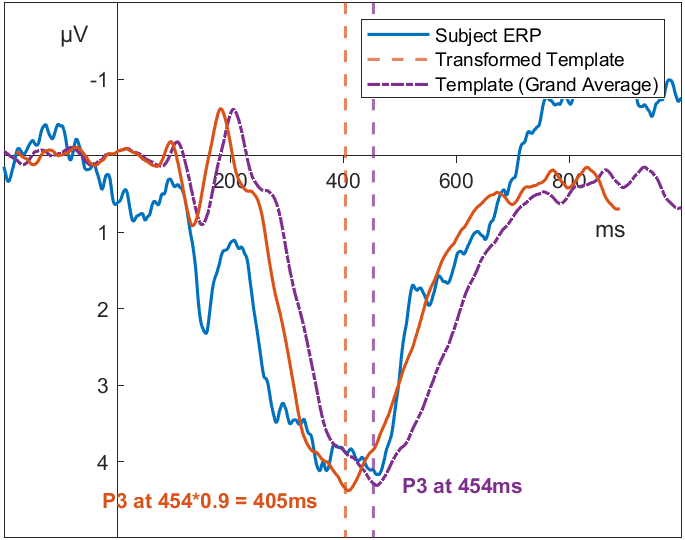
\includegraphics[width=2.28in]{../images/template_matching_example_introduction} \caption{Transforming the template to match an ERP}\label{fig:introduction-example-img}
\end{figure}

Optimization of these free parameters is based on so called \emph{similarity measures}. The similarity measure quantifies the fit of the transformed template to the subject-level signal. Different approaches to similarity measures are present in the template matching literature and fall into one of two camps: distance-based or correlation-based (\protect\hyperlink{ref-brunelli2009template}{Brunelli, 2009}; \protect\hyperlink{ref-mahalakshmi2012image}{Mahalakshmi et al., 2012}). These different approaches may result in different performance of the template matching algorithm (\protect\hyperlink{ref-brunelli1997template}{Brunelli \& Poggiot, 1997}; \protect\hyperlink{ref-goshtasby1984two}{Goshtasby et al., 1984}). We therefore implemented a version of both types of similarity measures. The first is based on minimizing the squared distance (MINSQ) and the second is based on maximizing the correlation between the transformed template and the signal (MAXCOR).

If used without any further modification, all points of the signal would contribute equally to the similarity measure. However, as the component of interest in the grand average only consists of a part of the signal and does not incorporate all points in time, we tested the use of weighting windows that weigh the similarity measure depending on the time of the component of interest in the grand average. When extracting P3 latencies, which usually occur around 300-500ms (\protect\hyperlink{ref-luck2014introduction}{Luck, 2014}), early and late activity in the grand average should not influence the template matching procedure as much as the activity central to the P3. Using these weighting windows helps the algorithm to more closely mirror human behavior. Similarly, researchers manually extracting latencies focus on those parts of the signal where the component of interest occurs.

A focus on specific parts of the signal is also present in peak and area latency algorithms. Here it is introduced by the use of measurement windows. Activity outside of these fixed windows is not considered in peak latency or fractional area latency algorithms. Additionally, these measurement windows are applied to each subject-level ERP and directly influence what part of the signal is included. In our template matching algorithm, these windows are based on the grand average and do not directly indicate what part of the subject-level signal is included. Rather, they influence the template that is used during the template matching algorithm. To underline this difference, we will refer to windows set in the context of the template matching algorithm as \emph{weighting windows}.

These weighting windows form the basis of a weighting vector used during the template matching procedure. Generally speaking, the difference (or correlation) between template and signal outside of that window is less important than the difference inside of the window.

\hypertarget{testing}{%
\subsection{Testing}\label{testing}}

We used the same data used by Sadus et al. (\protect\hyperlink{ref-sadus2024explorative}{2024}) and investigated both the psychometric properties of our new algorithm as well as the correlation with manually extracted latencies. This allows us to evaluate whether our new algorithm is a suitable replacement for the current gold-standard - manual extraction. Additionally, using data from this multiverse study allows us to investigate the impact of different tasks and pre-processing steps on the evaluated algorithms and provide insight into the conditions under which each algorithm performs best or worst.

We expanded this validation approach by a simulation study based on data used by Schubert et al. (\protect\hyperlink{ref-schubert2023robust}{2023}) in order to investigate how well a particular algorithm can recover a pre-specified true value. Since no simulation approach exists that can generate realistic ERPs with a known true latency, we simulated shifts in latency between experimental conditions similar to Kiesel et al. (\protect\hyperlink{ref-kiesel2008measurement}{2008}). We then evaluated how well peak latency, fractional area latency, and template matching algorithms recover those true simulated latency differences.

We hope to show that a template matching algorithm using the grand average as a variable template can successfully extract subject-level P3 component latencies. Ideally, use of this algorithm improves psychometric properties in comparison to prior algorithms, show high correlations with manually extracted data, accurately recover simulated latency shifts, and present an objective and efficient way to extract ERP latencies.

\hypertarget{template-matching-1}{%
\section{Template Matching}\label{template-matching-1}}

The template matching algorithm is implemented in MATLAB (Version 2024a)\footnote{Additionally, we use the Database Toolbox, the Optimization Toolbox, the Global Optimization Toolbox, the Parallel Computing Toolbox, and the Signal Processing Toolbox.}. Broadly, the algorithm can be divided into four steps: generation of the dynamic template, application of similarity weights, optimization, and recovery of latency from free parameters.

\hypertarget{template-generation}{%
\subsection{Template Generation}\label{template-generation}}

We use the grand average ERP over all participants as a template and introduce two free parameters to allow the template to match individual differences in amplitude and latency. Both parameters lead to linear transformations of the template. The first parameter \(a\) scales the entire template and adjusts for individual differences in amplitude. The second parameter \(b\) stretches or compresses the entire template and adjusts for individual differences in time course.

Implementation of the parameter \(a\) is straightforward: the entire template signal is multiplied by \(a\). This results in linear transformations of the template along the amplitude axis. To implement the parameter \(b\) that enables linear transformations along the time axis, we simply stretch or compress the signal along the x-axis. We then use spline interpolation to estimate the signal for a given transformed time-point. For example, if the template has a peak signal strength of \(9.4\ \mu V\) at 370 ms and the transformation parameter \(b = 1.1\), the transformed template will have the signal strength of \(9.4\ \mu V\) at \(370 \times 1.1\) ms. The signal strength at 370 ms will be equal to the spline interpolated signal strength of the untransformed template at \(\frac{370}{1.1}\) ms (see Figure \ref{fig:transformation-example-img}).



\begin{figure}
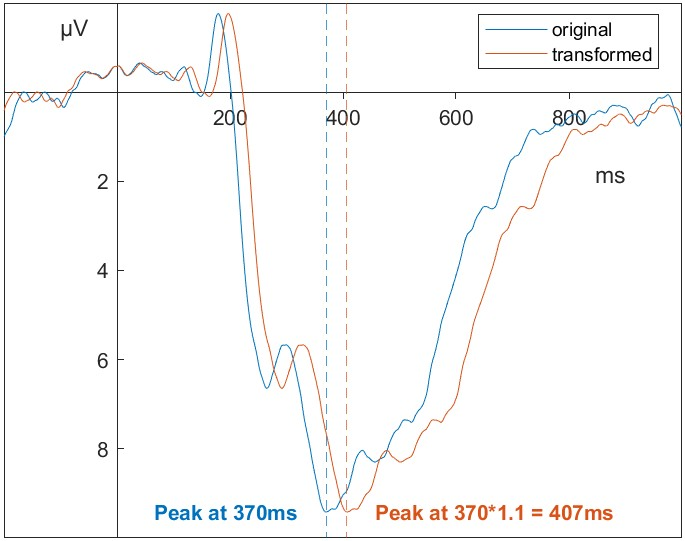
\includegraphics[width=2.28in]{../images/transformation_example} \caption{Transforming the latency of a signal using \(b\)}\label{fig:transformation-example-img}
\end{figure}

The algorithm allows these two free parameters to transform the template along the time- and amplitude-dimension and then optimizes the parameters for maximum similarity between the transformed template and subject-level ERP.

\hypertarget{similarity-measures}{%
\subsection{Similarity Measures}\label{similarity-measures}}

We chose to test two different approaches to similarity measures in this paper. The first approach minimizes the (weighted) squared distance between transformed template \(t(a, b)\) and the signal \(s\). It will be referred to as the MINSQ approach.

\[\underset{a, b}{\mathrm{argmin}} = \sum_i \omega_i(t_i(a, b) - s_i)^2.\]
The second approach aims to maximize the (weighted) correlation between transformed template \(t(a,b)\) and signal \(s\). It will be referred to as the MAXCOR approach.

\[\underset{a,b}{\mathrm{argmax}} = \frac{cov(t(a, b), s; \omega)}{\sqrt{cov(t(a, b), t(a, b); \omega)cov(s,s; \omega)}},\]
where
\[cov(t(a,b), s; \omega) = \frac{\sum_i \omega_i \cdot (t_i(a,b) - m(t(a, b); \omega))(s_i - m(s;\omega))}{\sum_i \omega_i},\]
and
\[m(t(a, b); \omega) = \frac{\sum_i \omega_i t_i(a,b)}{\sum_i \omega_i}.\]
However, since the parameter \(a\) linearly scales the template \(t_i(a, b)\) it can be rewritten as \(at_i(b)\). From this follows:

\[cov(t(a,b), s; \omega) = cov(at(b), s; \omega),\]
and thus
\[\frac{cov(t(a, b), s; \omega)}{\sqrt{cov(t(a, b), t(a, b); \omega)cov(s,s; \omega)}} = \frac{cov(at(b), s; \omega)}{\sqrt{cov(at(b), at(b); \omega)cov(s,s; \omega)}},\]
extracting \(a\) out of the covariance terms
\[\frac{cov(at(b), s; \omega)}{\sqrt{cov(at(b), at(b); \omega)cov(s,s; \omega)}} = \frac{acov(t(b), s; \omega)}{\sqrt{a^2cov(t(b), t(b); \omega)cov(s,s; \omega)}},\]
and finally
\[\frac{acov(t(b), s; \omega)}{\sqrt{a^2cov(t(b), t(b); \omega)cov(s,s; \omega)}} = \frac{cov(t(b), s; \omega)}{\sqrt{cov(t(b), t(b); \omega)cov(s,s; \omega)}}.\]
This shows that \(a\) does not impact the weighted correlation. We thus only optimized \(b\) when using the MAXCOR approach and set \(a = 1\).

\hypertarget{weighting-vectors}{%
\subsection{Weighting Vectors}\label{weighting-vectors}}

In order to impart weights on the matching procedure that allow placing more importance on those parts of the signal where the component of interest occurs, we use a weighting vector \(\omega\). Weighting windows indicate when the component of interest occurs.

We tested three different weighting windows in order to investigate which size leads to the best template matching results. We implemented the two measurement windows used in Sadus et al. (\protect\hyperlink{ref-sadus2024explorative}{2024}) in order to compare our results to theirs. The first window has a range from 250 ms to 700 ms and the second window has a range from 250 ms to 900 ms. In order to include some of the activity of earlier components, we also tested a weighting window from 200 ms to 700 ms.

Weighting windows are then combined with a weighting function to generate the weighting vector used in the template matching algorithm. A simple function to generate this weighting vector would be to assign 0 to all values outside of the window and 1 to all values inside of that window. This rectangular window would correspond to a Tukey window with \(\alpha\) = 0 (\protect\hyperlink{ref-bloomfield2004fourier}{Bloomfield, 2004}) and is also referred to as a Dirichlet window. The rectangular shape of this weighting window suggests a sudden drop in the relevance of a mismatch just at the weighting window's borders. However, such a sudden cut-off is difficult to justify. Therefore, we tested two versions of weighting functions that include tapered edges.

We tested a Tukey window with \(\alpha = 0.25\) and the Hamming window to slowly raise the weights from 0 outside of the measurement window to 1 inside the measurement window (\protect\hyperlink{ref-bloomfield2004fourier}{Bloomfield, 2004}). We also tested an additional weighting function that assigns weights based on the maximum-normalized amplitude of the grand average. Here the difference between transformed template and signal is of maximum importance at the peak of the component in the grand average and decreases in importance at lower amplitudes. See Figure \ref{fig:weighting-functions-overview-img} for an overview of the different weighting functions. Additional information about the weighting functions can be found in the Appendix / supplementary materials.



\begin{figure}
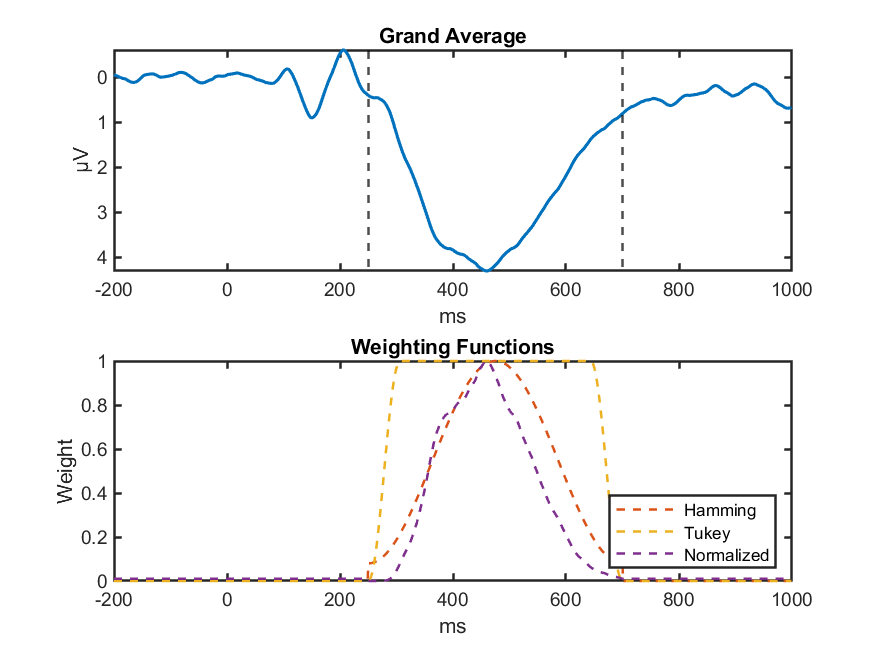
\includegraphics[width=2.92in]{../images/weighting_functions_overview} \caption{Overview of weighting functions}\label{fig:weighting-functions-overview-img}
\end{figure}

These weighting windows are defined based on the location of the component of interest in the grand average. In order to simplify the optimization, we chose to rescale the subject-level ERP along the time- and amplitude-dimension and fit it to the static grand average. Therefore, the actual implementation runs exactly opposite to the argument outlined here. This allows us to keep the weighting windows and weighting vectors constant and only transform the subject-level ERP signal. It has no impact on the fit statistic or the recovered latency.

\hypertarget{penalty}{%
\subsection{Penalty}\label{penalty}}

Additionally, we observed that the algorithms would sometimes converge on extreme values of the transformation parameter \(b\) if no clear solution can be found. To combat this, we also ran all combinations of similarity measures, weighting windows, and weighting functions with a penalty function that penalizes the MAXCOR and MINSQ function for \(b \le 0.\overline{6}\) or \(b \ge 1.5\) by multiplying the value of the function by \(e^b\) (or \(e^{\frac{1}{b}}\) for \(b < 1\)).

\hypertarget{optimization}{%
\subsection{Optimization}\label{optimization}}

All combinations of similarity measures, weighting windows, weighting functions, and penalty functions optimize the similarity measure using on the GlobalSearch algorithm (\protect\hyperlink{ref-ugray2007scatter}{Ugray et al., 2007}) implemented in the Global Optimization Toolbox (\protect\hyperlink{ref-matlab2024a}{The Math Works, 2024}). This optimization algorithm uses a multistart heuristic approach to find the global minimum of a nonlinear differentiable function by evaluating multiple starting points for local minima. We constrained the parameter \(a\) with lower and upper bounds of \([0.2, 20]\) and the parameter \(b\) with bounds of \([0.3, 2]\)\footnote{For the lower bound of \(b\), we chose a factor of three as this seemed more conservative to us. However, this is not optimal for the upper bound, as the signal is compressed by \(b\) in our implementation. This leads to \textgreater{} 50\% missing values in cases where \(b > 2\). Therefore, we chose 2 as the upper and 0.3 as the lower boundary. For the parameter \(a\), we chose 0.2 in order to prevent the algorithm to converge on a value close to 0 in cases with inconclusive signal. We added the upper bound of 20 as a very liberal bound on the factor by which the grand average may differ from the individual signal.}. The algorithm returns both the optimal parameters as well as the resulting optimal similarity measure.

\hypertarget{fit}{%
\subsection{Fit}\label{fit}}

The optimal similarity measure returned by the algorithm can be used as an indicator of certainty. Very close fits of transformed template to subject-level ERP suggest a high degree of certainty and low impact of noise. Poor similarity measures, like correlations \(r < 0.3\) suggest that even the optimal transformation of the component in the template does not closely resemble the component structure in the subject-level ERP. Therefore, we used of this fit statistic to remove latency estimates where even the best fit shows poor similarity between template and signal. Because the (weighted) correlation is easier to interpret, we used the correlation as an indicator of fit for both the MAXCOR and MINSQ approach and removed those latency estimates with correlations \(r < 0.3\).

\hypertarget{recovery-of-component-latency}{%
\subsection{Recovery of component latency}\label{recovery-of-component-latency}}

We can use the set of optimal transformation parameters to recover the latency of subject-level ERPs. Prior to this, the latency of the component of interest in the grand average needs to be quantified. This can be done either manually or using one of the standard algorithms, like peak latency or fractional area latency. Due to the high signal-to-noise ratio of the grand average, applying these algorithms is much less problematic than in noisy subject-level ERPs. In our analysis, we use the 50\% area latency algorithm proposed by Liesefeld (\protect\hyperlink{ref-liesefeld2018estimating}{2018}) with the respective weighting window as a measurement window to determine the latency in the grand average.

The latency of the component in the grand average \(l_{GA}\) is then multiplied by the optimal latency shift parameter of subject \(j\) to obtain the latency in the subject-level ERP,

\[l_{GA} \cdot b_j = l_{j}.\]

\hypertarget{other-extraction-methods}{%
\subsection{Other extraction methods}\label{other-extraction-methods}}

We defined peak latency as the time of maximum positive voltage deflection within a fixed measurement window which is also larger than the average of the three points both to the right as well as to the left of it (\protect\hyperlink{ref-luck2014introduction}{Luck, 2014}).

We determined fractional area latency using the 50\% area latency approach. All signal below 0 was set to 0. Then we summed up the signal within the measurement window and extracted the two time-points between which the signal grows larger than 50\% of the total. The exact latency was then determined through linear interpolation.

We also tested the modifications to fractional area latency suggested by Liesefeld (\protect\hyperlink{ref-liesefeld2018estimating}{2018}) and subtracted half of the maximum amplitude from the signal as a relative baseline (see also \protect\hyperlink{ref-wascher2022mental}{Wascher et al., 2022}). Essentially, we set all signal below 50\% of the maximum amplitude to 0. All other steps were identical to the steps taken in the regular 50\% area latency algorithm.

\hypertarget{study-1}{%
\section{Study 1}\label{study-1}}

\hypertarget{method}{%
\subsection{Method}\label{method}}

All analyses presented here are based on data originally published in Löffler et al. (\protect\hyperlink{ref-loffler2024common}{2024}). The original data contain EEG recordings from 6 different tasks. We focused on the same three tasks that have been already selected by Sadus et al. (\protect\hyperlink{ref-sadus2024explorative}{2024}).

\hypertarget{participants}{%
\subsubsection{Participants}\label{participants}}

The empirical evaluation of our algorithm that is presented in the first part of this paper follows Sadus et al. (\protect\hyperlink{ref-sadus2024explorative}{2024}). Their analysis used a sample of 30 young (18-21 years old, \(M_{age}\) = 19.37, \(SD_{age}\) = 0.76) and 30 old participants (50-60 years old, \(M_{age}\) = 55.83, \(SD_{age}\) = 2.87), representing the 30 youngest and 30 oldest participants from the overall study (\protect\hyperlink{ref-loffler2024common}{Löffler et al., 2024}).

All participants had normal or corrected to normal vision. None of the participants had neurological or mental disorders, used psychotropic drugs, wore a pacemaker or suffered from red-green color vision deficiency. All participants provided informed consent prior to participation and received 75€ or course credit for participation.

\hypertarget{tasks}{%
\subsubsection{Tasks}\label{tasks}}

All participants completed a set of three tasks: a Flanker Task, an Nback Task, and a Switching Task. Each assesses one of the executive functions proposed by Miyake et al. (\protect\hyperlink{ref-miyake2000unity}{2000}). Löffler et al. (\protect\hyperlink{ref-loffler2024common}{2024}) programmed all tasks using MATLAB (\protect\hyperlink{ref-matlab2022b}{The Math Works, 2022}) and the software package Psychtoolbox (Version 3-0.13) (\protect\hyperlink{ref-brainard1997psychophysics}{Brainard \& Vision, 1997}; \protect\hyperlink{ref-kleiner2007psychtoolbox}{Kleiner et al., 2007}; \protect\hyperlink{ref-pelli1997videotoolbox}{Pelli \& Vision, 1997}). We presented stimuli centrally against a black background and instructed participants to respond as quickly and accurately as possible.

\hypertarget{flanker-task}{%
\paragraph{Flanker Task}\label{flanker-task}}

We employed a standard Arrow Flanker task (\protect\hyperlink{ref-eriksen1974effects}{Eriksen \& Eriksen, 1974}) to evaluate a participant's \emph{inhibition} ability. A central arrow was flanked by additional arrows appeared on the screen, with the flanking arrows either pointing in the same or opposite direction to the central arrow. All participants had to identify the direction of the central arrow while ignoring the flanking arrows. Each participant completed practice trials followed by 100 congruent and 100 incongruent trials.

\hypertarget{nback-task}{%
\paragraph{Nback Task}\label{nback-task}}

An adapted Nback task (\protect\hyperlink{ref-scharinger2015flanker}{Scharinger et al., 2015}) assessed participants' \emph{updating} abilities. During presentation of a stream of letters, participants had to indicate whether the current letter matched either a predefined target-letter (0-back condition) or the letter presented immediately before (1-back condition). In the original study, participants also completed a 2-back condition. Following Sadus et al. (\protect\hyperlink{ref-sadus2024explorative}{2024}), we excluded this condition from the analysis. All participants completed practice trials and 96 trials per condition.

\hypertarget{switching-task}{%
\paragraph{Switching Task}\label{switching-task}}

We administered a Switching task to measure participants' \emph{shifting} ability. We presented colored digits ranging from 1 to 9. Participants had to categorize them based on predefined rules signaled by a colored fixation cross before each trial. They had to either indicate whether the digit was greater than or less than 5 or whether the digit was odd or even. Participants either maintained the same rule as the previous trial or switched to the alternate rule. Each participant completed practice trials followed by 192 trials in both the repeat and switch conditions.

\hypertarget{procedure}{%
\subsubsection{Procedure}\label{procedure}}

The original study consisted of three test sessions. The three tasks analyzed here were all conducted in the first session. The original study included two additional measurement occasions which we will not discuss further here. During EEG measurement, participants were seated approximately 140 cm from a monitor in a sound-attenuated room.

\hypertarget{eeg-recording-and-processing}{%
\subsubsection{EEG recording and processing}\label{eeg-recording-and-processing}}

We continuously recorded EEG data using 32 equidistant Ag/AgCl electrodes and took additional electrooculogram (EOG) measures with two electrodes placed above and below the left eye to correct for ocular artifacts. We maintained all impedances below 5 kΩ. We recorded the signal with a sampling rate of 1000 Hz and online-referenced it to Cz. We removed artifacts using ICA on a cloned dataset down-sampled to 200 Hz and filtered with a high-pass filter of 1 Hz. We further removed line-noise using the CleanLine function (\protect\hyperlink{ref-mullen2012cleanline}{Mullen, 2012}). We detected bad channels using a z-value threshold of 3.29 as per the EPOS pipeline (\protect\hyperlink{ref-rodrigues2021epos}{Rodrigues et al., 2021}) and interpolated channels that were removed following this procedure. Then, we re-referenced the data using an average referencing scheme. Based on a threshold of \(1000 \ \mu V\) and excluding data more than 5 SDs away from the mean, we automatically detected and removed a maximum of 5\% of segments per iteration containing artifacts in the ICA-dataset. We used the InfoMax algorithm in the ICA and applied the resulting decomposition to the original dataset. We removed ICs determined to be less than 50\% likely to be brain activity by the ICLabel Algorithm (\protect\hyperlink{ref-pion2019iclabel}{Pion-Tonachini et al., 2019}). Then, we low-pass filtered the data using a Butterworth filter with varying cutoff frequencies (4 Hz, 8 Hz, 16 Hz, 32 Hz, and no filter) and segmented it into 1200 ms epochs starting 200 ms prior to stimulus onset. Again, we automatically detected and removed segments containing artifacts. Finally, we baseline corrected segments using the 200 ms prior to stimulus onset. We conducted ERP analyses in MATLAB (Version 2024a) (\protect\hyperlink{ref-matlab2024a}{The Math Works, 2024}). We only included correct trials in the analysis and investigated the P3 at the electrode Pz in accordance with existing literature (\protect\hyperlink{ref-polich2012neuropsychology}{Polich, 2012}; \protect\hyperlink{ref-verleger2020effects}{Verleger, 2020}).

\hypertarget{latency-extraction-techniques}{%
\subsubsection{Latency extraction techniques}\label{latency-extraction-techniques}}

We compared all versions of a template matching algorithm resulting from the combinations of similarity measures, weighting windows, weighting functions, and penalty methods to traditional approaches such as peak latency, fractional area latency, and the fractional area latency algorithm proposed by Liesefeld (\protect\hyperlink{ref-liesefeld2018estimating}{2018}). For peak latency and 50\% area latency algorithms, we used the respective measurement windows used by Sadus et al. (\protect\hyperlink{ref-sadus2024explorative}{2024}). See Figure \ref{fig:method-overview-img} for an overview.



\begin{figure}
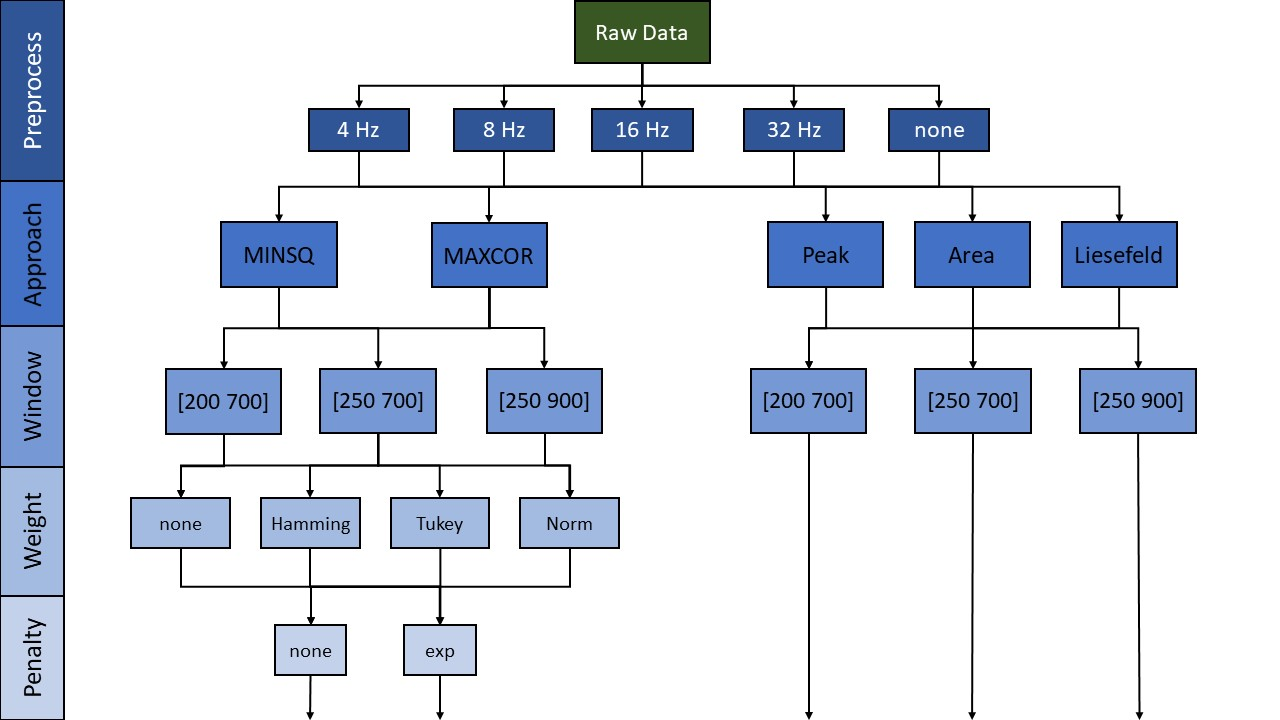
\includegraphics[width=4.27in]{../images/method_overview} \caption{Overview of extraction algorithms}\label{fig:method-overview-img}
\end{figure}

\hypertarget{empirical-evaluation}{%
\subsubsection{Empirical evaluation}\label{empirical-evaluation}}

In order to compare our newly proposed algorithm to existing extraction methods, we applied all versions of the template matching algorithm as well as the peak latency algorithm, the 50\% area latency algorithm, and the modified area latency algorithm (\protect\hyperlink{ref-liesefeld2018estimating}{Liesefeld, 2018}; \protect\hyperlink{ref-wascher2022mental}{Wascher et al., 2022}). We focused on the reliability of latency values that are extracted by a particular algorithm and the intra-class correlation of latencies extracted by an algorithm vs.~an expert ERP researcher (i.e.~we used the manually extracted latencies from; (\protect\hyperlink{ref-sadus2024explorative}{Sadus et al., 2024}).

\hypertarget{results}{%
\subsection{Results}\label{results}}

We conducted all data preprocessing and statistical analyses using R {[}Version 4.3.0; R Core Team (\protect\hyperlink{ref-R-base}{2022}){]}\footnote{We, furthermore, used the R-packages \emph{afex} (Version 1.3.1; \protect\hyperlink{ref-R-afex}{Singmann et al., 2023}), \emph{emmeans} (Version 1.10.2; \protect\hyperlink{ref-R-emmeans}{Lenth, 2023}), \emph{flextable} (Version 0.9.6; \protect\hyperlink{ref-R-flextable}{Gohel \& Skintzos, 2023}), \emph{knitr} (Version 1.46; \protect\hyperlink{ref-R-knitr}{Xie, 2015}), \emph{papaja} (Version 0.1.2; \protect\hyperlink{ref-R-papaja}{Aust \& Barth, 2022}), \emph{rmarkdown} (Version 2.26; \protect\hyperlink{ref-R-rmarkdown_a}{Xie et al., 2018}, \protect\hyperlink{ref-R-rmarkdown_b}{2020}), and \emph{tidyverse} (Version 2.0.0; \protect\hyperlink{ref-R-tidyverse}{Wickham et al., 2019}).}.

The grand averages for the three tasks in the empirical evaluation and the data containing the full set of participants used in the simulation are displayed in Figure \ref{fig:grand-average-plots}.



\begin{figure}
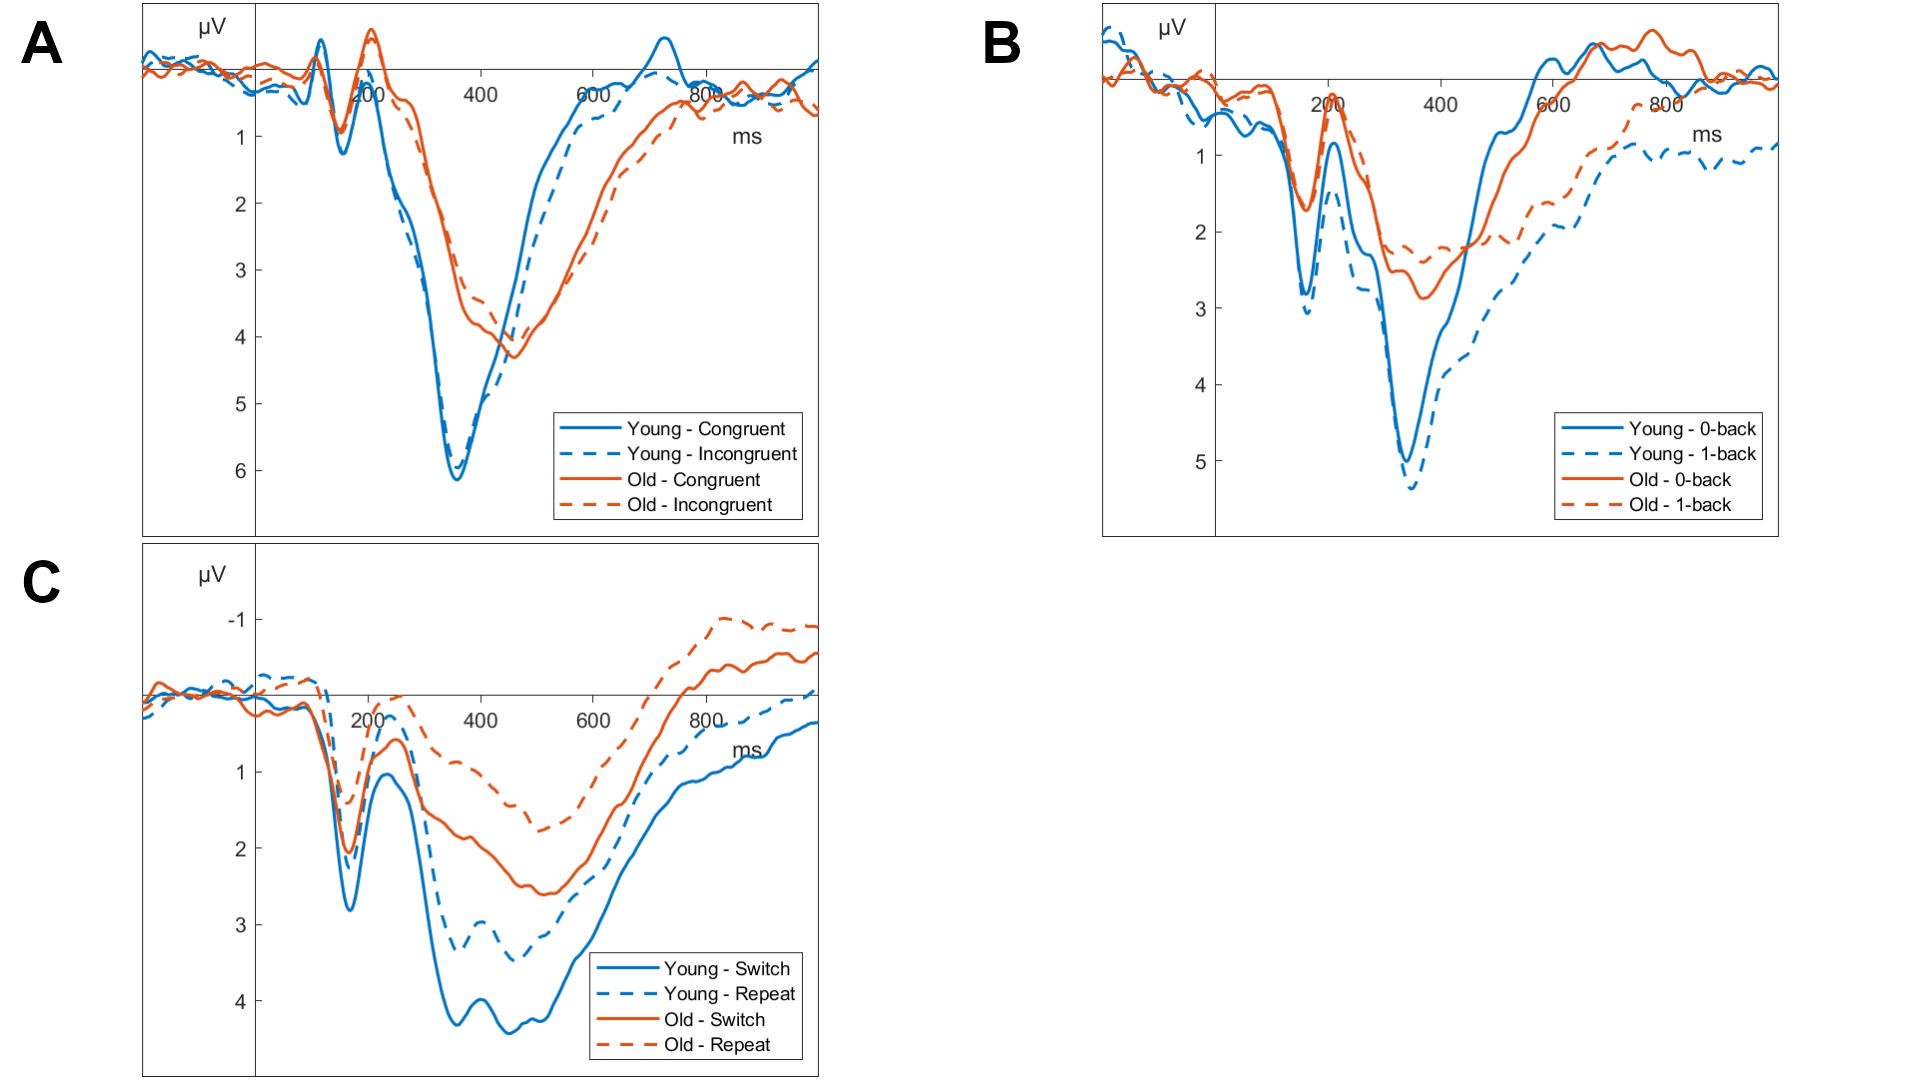
\includegraphics[width=6.4in]{../images/arranged_img_ga} \caption{Grand Averages of the Tasks used at Pz with a 32 Hz low-pass filter}\label{fig:grand-average-plots}
\end{figure}

\hypertarget{descriptive-statistics}{%
\subsubsection{Descriptive Statistics}\label{descriptive-statistics}}

The percentage of missing values varied systematically depending on the extraction algorithm (see Table \ref{tab:overview-table-missing-kathrin}). Across tasks, preprocessing steps, weighting windows, weighting functions, and without a penalty the MINSQ algorithm resulted in 20.00 \% missing values and the MAXCOR algorithm in 11.00 \% missing values. Penalizing more extreme transformation parameters reduced the percentage of missing values to 5.54 \% for the MINSQ algorithm and 3.15 \% for the MAXCOR algorithm. The peak latency algorithm resulted in 0.00 \% missing values, with 2.17 \% and 2.33 \% missing values for the area latency and modified area latency algorithm, respectively. For reference, the expert ERP researcher in Sadus et al. (\protect\hyperlink{ref-sadus2024explorative}{2024}) classified 4.05 \% of individual ERPs as missing values.



\global\setlength{\Oldarrayrulewidth}{\arrayrulewidth}

\global\setlength{\Oldtabcolsep}{\tabcolsep}

\setlength{\tabcolsep}{2pt}

\renewcommand*{\arraystretch}{1.5}

\begin{table}

\providecommand{\ascline}[3]{\noalign{\global\arrayrulewidth #1}\arrayrulecolor[HTML]{#2}\cline{#3}}

\begin{longtable}[l]{cccccccc}

\caption{Missing values for different algorithms: empirical evaluation}\label{tab:overview-table-missing-kathrin}\\

\ascline{1.5pt}{666666}{1-8}

\multicolumn{1}{>{}l}{} & \multicolumn{1}{>{}l}{} & \multicolumn{2}{>{}c}{\textcolor[HTML]{000000}{\fontsize{11}{6}\selectfont{[200\ 700]}}} & \multicolumn{2}{>{}c}{\textcolor[HTML]{000000}{\fontsize{11}{6}\selectfont{[250\ 700]}}} & \multicolumn{2}{>{}c}{\textcolor[HTML]{000000}{\fontsize{11}{6}\selectfont{[250\ 900]}}} \\





\multicolumn{1}{>{}l}{\multirow[b]{-2}{*}{\parbox{0.75in}{\raggedright \textcolor[HTML]{000000}{\fontsize{11}{6}\selectfont{approach}}}}} & \multicolumn{1}{>{}l}{\multirow[b]{-2}{*}{\parbox{0.75in}{\raggedright \textcolor[HTML]{000000}{\fontsize{11}{6}\selectfont{weight}}}}} & \multicolumn{1}{>{}c}{\textcolor[HTML]{000000}{\fontsize{11}{6}\selectfont{penalized}}} & \multicolumn{1}{>{}c}{\textcolor[HTML]{000000}{\fontsize{11}{6}\selectfont{none}}} & \multicolumn{1}{>{}c}{\textcolor[HTML]{000000}{\fontsize{11}{6}\selectfont{penalized}}} & \multicolumn{1}{>{}c}{\textcolor[HTML]{000000}{\fontsize{11}{6}\selectfont{none}}} & \multicolumn{1}{>{}c}{\textcolor[HTML]{000000}{\fontsize{11}{6}\selectfont{penalized}}} & \multicolumn{1}{>{}c}{\textcolor[HTML]{000000}{\fontsize{11}{6}\selectfont{none}}} \\

\ascline{1.5pt}{666666}{1-8}\endfirsthead \caption[]{Missing values for different algorithms: empirical evaluation}\label{tab:overview-table-missing-kathrin}\\

\ascline{1.5pt}{666666}{1-8}

\multicolumn{1}{>{}l}{} & \multicolumn{1}{>{}l}{} & \multicolumn{2}{>{}c}{\textcolor[HTML]{000000}{\fontsize{11}{6}\selectfont{[200\ 700]}}} & \multicolumn{2}{>{}c}{\textcolor[HTML]{000000}{\fontsize{11}{6}\selectfont{[250\ 700]}}} & \multicolumn{2}{>{}c}{\textcolor[HTML]{000000}{\fontsize{11}{6}\selectfont{[250\ 900]}}} \\





\multicolumn{1}{>{}l}{\multirow[b]{-2}{*}{\parbox{0.75in}{\raggedright \textcolor[HTML]{000000}{\fontsize{11}{6}\selectfont{approach}}}}} & \multicolumn{1}{>{}l}{\multirow[b]{-2}{*}{\parbox{0.75in}{\raggedright \textcolor[HTML]{000000}{\fontsize{11}{6}\selectfont{weight}}}}} & \multicolumn{1}{>{}c}{\textcolor[HTML]{000000}{\fontsize{11}{6}\selectfont{penalized}}} & \multicolumn{1}{>{}c}{\textcolor[HTML]{000000}{\fontsize{11}{6}\selectfont{none}}} & \multicolumn{1}{>{}c}{\textcolor[HTML]{000000}{\fontsize{11}{6}\selectfont{penalized}}} & \multicolumn{1}{>{}c}{\textcolor[HTML]{000000}{\fontsize{11}{6}\selectfont{none}}} & \multicolumn{1}{>{}c}{\textcolor[HTML]{000000}{\fontsize{11}{6}\selectfont{penalized}}} & \multicolumn{1}{>{}c}{\textcolor[HTML]{000000}{\fontsize{11}{6}\selectfont{none}}} \\

\ascline{1.5pt}{666666}{1-8}\endhead



\multicolumn{1}{>{}l}{} & \multicolumn{1}{>{}l}{\textcolor[HTML]{000000}{\fontsize{11}{6}\selectfont{none}}} & \multicolumn{1}{>{}c}{\textcolor[HTML]{000000}{\fontsize{11}{6}\selectfont{0.05}}} & \multicolumn{1}{>{}c}{\textcolor[HTML]{000000}{\fontsize{11}{6}\selectfont{0.08}}} & \multicolumn{1}{>{}c}{\textcolor[HTML]{000000}{\fontsize{11}{6}\selectfont{0.05}}} & \multicolumn{1}{>{}c}{\textcolor[HTML]{000000}{\fontsize{11}{6}\selectfont{0.08}}} & \multicolumn{1}{>{}c}{\textcolor[HTML]{000000}{\fontsize{11}{6}\selectfont{0.05}}} & \multicolumn{1}{>{}c}{\textcolor[HTML]{000000}{\fontsize{11}{6}\selectfont{0.08}}} \\





\multicolumn{1}{>{}l}{} & \multicolumn{1}{>{}l}{\textcolor[HTML]{000000}{\fontsize{11}{6}\selectfont{hamming}}} & \multicolumn{1}{>{}c}{\textcolor[HTML]{000000}{\fontsize{11}{6}\selectfont{0.03}}} & \multicolumn{1}{>{}c}{\textcolor[HTML]{000000}{\fontsize{11}{6}\selectfont{0.16}}} & \multicolumn{1}{>{}c}{\textcolor[HTML]{000000}{\fontsize{11}{6}\selectfont{0.02}}} & \multicolumn{1}{>{}c}{\textcolor[HTML]{000000}{\fontsize{11}{6}\selectfont{0.17}}} & \multicolumn{1}{>{}c}{\textcolor[HTML]{000000}{\fontsize{11}{6}\selectfont{0.04}}} & \multicolumn{1}{>{}c}{\textcolor[HTML]{000000}{\fontsize{11}{6}\selectfont{0.08}}} \\





\multicolumn{1}{>{}l}{} & \multicolumn{1}{>{}l}{\textcolor[HTML]{000000}{\fontsize{11}{6}\selectfont{tukey}}} & \multicolumn{1}{>{}c}{\textcolor[HTML]{000000}{\fontsize{11}{6}\selectfont{0.03}}} & \multicolumn{1}{>{}c}{\textcolor[HTML]{000000}{\fontsize{11}{6}\selectfont{0.15}}} & \multicolumn{1}{>{}c}{\textcolor[HTML]{000000}{\fontsize{11}{6}\selectfont{0.03}}} & \multicolumn{1}{>{}c}{\textcolor[HTML]{000000}{\fontsize{11}{6}\selectfont{0.15}}} & \multicolumn{1}{>{}c}{\textcolor[HTML]{000000}{\fontsize{11}{6}\selectfont{0.04}}} & \multicolumn{1}{>{}c}{\textcolor[HTML]{000000}{\fontsize{11}{6}\selectfont{0.08}}} \\





\multicolumn{1}{>{}l}{\multirow[c]{-4}{*}{\parbox{0.75in}{\raggedright \textcolor[HTML]{000000}{\fontsize{11}{6}\selectfont{maxcor}}}}} & \multicolumn{1}{>{}l}{\textcolor[HTML]{000000}{\fontsize{11}{6}\selectfont{normalized}}} & \multicolumn{1}{>{}c}{\textcolor[HTML]{000000}{\fontsize{11}{6}\selectfont{0.01}}} & \multicolumn{1}{>{}c}{\textcolor[HTML]{000000}{\fontsize{11}{6}\selectfont{0.10}}} & \multicolumn{1}{>{}c}{\textcolor[HTML]{000000}{\fontsize{11}{6}\selectfont{0.01}}} & \multicolumn{1}{>{}c}{\textcolor[HTML]{000000}{\fontsize{11}{6}\selectfont{0.10}}} & \multicolumn{1}{>{}c}{\textcolor[HTML]{000000}{\fontsize{11}{6}\selectfont{0.01}}} & \multicolumn{1}{>{}c}{\textcolor[HTML]{000000}{\fontsize{11}{6}\selectfont{0.10}}} \\

\ascline{1pt}{666666}{1-8}



\multicolumn{1}{>{}l}{} & \multicolumn{1}{>{}l}{\textcolor[HTML]{000000}{\fontsize{11}{6}\selectfont{none}}} & \multicolumn{1}{>{}c}{\textcolor[HTML]{000000}{\fontsize{11}{6}\selectfont{0.06}}} & \multicolumn{1}{>{}c}{\textcolor[HTML]{000000}{\fontsize{11}{6}\selectfont{0.21}}} & \multicolumn{1}{>{}c}{\textcolor[HTML]{000000}{\fontsize{11}{6}\selectfont{0.06}}} & \multicolumn{1}{>{}c}{\textcolor[HTML]{000000}{\fontsize{11}{6}\selectfont{0.21}}} & \multicolumn{1}{>{}c}{\textcolor[HTML]{000000}{\fontsize{11}{6}\selectfont{0.06}}} & \multicolumn{1}{>{}c}{\textcolor[HTML]{000000}{\fontsize{11}{6}\selectfont{0.21}}} \\





\multicolumn{1}{>{}l}{} & \multicolumn{1}{>{}l}{\textcolor[HTML]{000000}{\fontsize{11}{6}\selectfont{hamming}}} & \multicolumn{1}{>{}c}{\textcolor[HTML]{000000}{\fontsize{11}{6}\selectfont{0.05}}} & \multicolumn{1}{>{}c}{\textcolor[HTML]{000000}{\fontsize{11}{6}\selectfont{0.19}}} & \multicolumn{1}{>{}c}{\textcolor[HTML]{000000}{\fontsize{11}{6}\selectfont{0.04}}} & \multicolumn{1}{>{}c}{\textcolor[HTML]{000000}{\fontsize{11}{6}\selectfont{0.19}}} & \multicolumn{1}{>{}c}{\textcolor[HTML]{000000}{\fontsize{11}{6}\selectfont{0.09}}} & \multicolumn{1}{>{}c}{\textcolor[HTML]{000000}{\fontsize{11}{6}\selectfont{0.25}}} \\





\multicolumn{1}{>{}l}{} & \multicolumn{1}{>{}l}{\textcolor[HTML]{000000}{\fontsize{11}{6}\selectfont{tukey}}} & \multicolumn{1}{>{}c}{\textcolor[HTML]{000000}{\fontsize{11}{6}\selectfont{0.07}}} & \multicolumn{1}{>{}c}{\textcolor[HTML]{000000}{\fontsize{11}{6}\selectfont{0.22}}} & \multicolumn{1}{>{}c}{\textcolor[HTML]{000000}{\fontsize{11}{6}\selectfont{0.06}}} & \multicolumn{1}{>{}c}{\textcolor[HTML]{000000}{\fontsize{11}{6}\selectfont{0.21}}} & \multicolumn{1}{>{}c}{\textcolor[HTML]{000000}{\fontsize{11}{6}\selectfont{0.09}}} & \multicolumn{1}{>{}c}{\textcolor[HTML]{000000}{\fontsize{11}{6}\selectfont{0.25}}} \\





\multicolumn{1}{>{}l}{\multirow[c]{-4}{*}{\parbox{0.75in}{\raggedright \textcolor[HTML]{000000}{\fontsize{11}{6}\selectfont{minsq}}}}} & \multicolumn{1}{>{}l}{\textcolor[HTML]{000000}{\fontsize{11}{6}\selectfont{normalized}}} & \multicolumn{1}{>{}c}{\textcolor[HTML]{000000}{\fontsize{11}{6}\selectfont{0.02}}} & \multicolumn{1}{>{}c}{\textcolor[HTML]{000000}{\fontsize{11}{6}\selectfont{0.15}}} & \multicolumn{1}{>{}c}{\textcolor[HTML]{000000}{\fontsize{11}{6}\selectfont{0.03}}} & \multicolumn{1}{>{}c}{\textcolor[HTML]{000000}{\fontsize{11}{6}\selectfont{0.15}}} & \multicolumn{1}{>{}c}{\textcolor[HTML]{000000}{\fontsize{11}{6}\selectfont{0.03}}} & \multicolumn{1}{>{}c}{\textcolor[HTML]{000000}{\fontsize{11}{6}\selectfont{0.16}}} \\

\ascline{1pt}{666666}{1-8}



\multicolumn{1}{>{}l}{\textcolor[HTML]{000000}{\fontsize{11}{6}\selectfont{peak}}} & \multicolumn{1}{>{}l}{\textcolor[HTML]{000000}{\fontsize{11}{6}\selectfont{none}}} & \multicolumn{1}{>{}c}{\textcolor[HTML]{000000}{\fontsize{11}{6}\selectfont{}}} & \multicolumn{1}{>{}c}{\textcolor[HTML]{000000}{\fontsize{11}{6}\selectfont{0.00}}} & \multicolumn{1}{>{}c}{\textcolor[HTML]{000000}{\fontsize{11}{6}\selectfont{}}} & \multicolumn{1}{>{}c}{\textcolor[HTML]{000000}{\fontsize{11}{6}\selectfont{0.00}}} & \multicolumn{1}{>{}c}{\textcolor[HTML]{000000}{\fontsize{11}{6}\selectfont{}}} & \multicolumn{1}{>{}c}{\textcolor[HTML]{000000}{\fontsize{11}{6}\selectfont{0.00}}} \\





\multicolumn{1}{>{}l}{\textcolor[HTML]{000000}{\fontsize{11}{6}\selectfont{area}}} & \multicolumn{1}{>{}l}{\textcolor[HTML]{000000}{\fontsize{11}{6}\selectfont{none}}} & \multicolumn{1}{>{}c}{\textcolor[HTML]{000000}{\fontsize{11}{6}\selectfont{}}} & \multicolumn{1}{>{}c}{\textcolor[HTML]{000000}{\fontsize{11}{6}\selectfont{0.02}}} & \multicolumn{1}{>{}c}{\textcolor[HTML]{000000}{\fontsize{11}{6}\selectfont{}}} & \multicolumn{1}{>{}c}{\textcolor[HTML]{000000}{\fontsize{11}{6}\selectfont{0.02}}} & \multicolumn{1}{>{}c}{\textcolor[HTML]{000000}{\fontsize{11}{6}\selectfont{}}} & \multicolumn{1}{>{}c}{\textcolor[HTML]{000000}{\fontsize{11}{6}\selectfont{0.02}}} \\





\multicolumn{1}{>{}l}{\textcolor[HTML]{000000}{\fontsize{11}{6}\selectfont{liesefeld}}} & \multicolumn{1}{>{}l}{\textcolor[HTML]{000000}{\fontsize{11}{6}\selectfont{none}}} & \multicolumn{1}{>{}c}{\textcolor[HTML]{000000}{\fontsize{11}{6}\selectfont{}}} & \multicolumn{1}{>{}c}{\textcolor[HTML]{000000}{\fontsize{11}{6}\selectfont{0.02}}} & \multicolumn{1}{>{}c}{\textcolor[HTML]{000000}{\fontsize{11}{6}\selectfont{}}} & \multicolumn{1}{>{}c}{\textcolor[HTML]{000000}{\fontsize{11}{6}\selectfont{0.02}}} & \multicolumn{1}{>{}c}{\textcolor[HTML]{000000}{\fontsize{11}{6}\selectfont{}}} & \multicolumn{1}{>{}c}{\textcolor[HTML]{000000}{\fontsize{11}{6}\selectfont{0.02}}} \\

\ascline{1.5pt}{666666}{1-8}



\multicolumn{8}{>{}l}{\textcolor[HTML]{000000}{\fontsize{11}{6}\selectfont{\textit{Note.\ }}}\textcolor[HTML]{000000}{\fontsize{11}{6}\selectfont{Frequency\ of\ missing\ values\ per\ algorithm.\ The\ rows\ indicate\ combinations\ of\ similarity\ measure\ and\ weighting\ function.\ The\ columns\ denote\ the\ measurement\ window\ and\ indicate\ if\ a\ penalty\ was\ used.}}} \\





\end{longtable}

\end{table}

\arrayrulecolor[HTML]{000000}

\global\setlength{\arrayrulewidth}{\Oldarrayrulewidth}

\global\setlength{\tabcolsep}{\Oldtabcolsep}

\renewcommand*{\arraystretch}{1}

\hypertarget{reliability}{%
\subsubsection{Reliability}\label{reliability}}

The reliability coefficients estimated using split-half correlations are reported in Table \ref{tab:overview-table-rel-kathrin}. Across tasks and preprocessing steps, the 50\% area latency algorithm with the window used in Sadus et al. (\protect\hyperlink{ref-sadus2024explorative}{2024}) (250 ms - 700 ms) resulted in the highest average reliability (\(r_{tt}~=~0.91\)). Across tasks, preprocessing steps, weighting windows, weighting functions, and penalty settings, the MINSQ algorithm showed a mean reliability of \(r_{tt}~=~0.88\) and the MAXCOR algorithm a mean reliability of \(r_{tt}~=~0.87\). The best reliability for the template matching algorithms was achieved when using the MAXCOR algorithm with no weights and an exponential penalty (\(r_{tt}~=~0.89\)) or the MINSQ algorithm with normalized weights and an exponential penalty (\(r_{tt}~=~0.89\)). The modified fractional area latency algorithm resulted in an average reliability of \(r_{tt}~=~0.90\) and the peak latency algorithm in an average reliability of \(r_{tt}~=~0.78\).



\global\setlength{\Oldarrayrulewidth}{\arrayrulewidth}

\global\setlength{\Oldtabcolsep}{\tabcolsep}

\setlength{\tabcolsep}{2pt}

\renewcommand*{\arraystretch}{1.5}

\begin{table}

\providecommand{\ascline}[3]{\noalign{\global\arrayrulewidth #1}\arrayrulecolor[HTML]{#2}\cline{#3}}

\begin{longtable}[l]{cccccccc}

\caption{Reliability for different algorithms: empirical evaluation}\label{tab:overview-table-rel-kathrin}\\

\ascline{1.5pt}{666666}{1-8}

\multicolumn{1}{>{}l}{} & \multicolumn{1}{>{}l}{} & \multicolumn{2}{>{}c}{\textcolor[HTML]{000000}{\fontsize{11}{6}\selectfont{[200\ 700]}}} & \multicolumn{2}{>{}c}{\textcolor[HTML]{000000}{\fontsize{11}{6}\selectfont{[250\ 700]}}} & \multicolumn{2}{>{}c}{\textcolor[HTML]{000000}{\fontsize{11}{6}\selectfont{[250\ 900]}}} \\





\multicolumn{1}{>{}l}{\multirow[b]{-2}{*}{\parbox{0.75in}{\raggedright \textcolor[HTML]{000000}{\fontsize{11}{6}\selectfont{approach}}}}} & \multicolumn{1}{>{}l}{\multirow[b]{-2}{*}{\parbox{0.75in}{\raggedright \textcolor[HTML]{000000}{\fontsize{11}{6}\selectfont{weight}}}}} & \multicolumn{1}{>{}c}{\textcolor[HTML]{000000}{\fontsize{11}{6}\selectfont{penalized}}} & \multicolumn{1}{>{}c}{\textcolor[HTML]{000000}{\fontsize{11}{6}\selectfont{none}}} & \multicolumn{1}{>{}c}{\textcolor[HTML]{000000}{\fontsize{11}{6}\selectfont{penalized}}} & \multicolumn{1}{>{}c}{\textcolor[HTML]{000000}{\fontsize{11}{6}\selectfont{none}}} & \multicolumn{1}{>{}c}{\textcolor[HTML]{000000}{\fontsize{11}{6}\selectfont{penalized}}} & \multicolumn{1}{>{}c}{\textcolor[HTML]{000000}{\fontsize{11}{6}\selectfont{none}}} \\

\ascline{1.5pt}{666666}{1-8}\endfirsthead \caption[]{Reliability for different algorithms: empirical evaluation}\label{tab:overview-table-rel-kathrin}\\

\ascline{1.5pt}{666666}{1-8}

\multicolumn{1}{>{}l}{} & \multicolumn{1}{>{}l}{} & \multicolumn{2}{>{}c}{\textcolor[HTML]{000000}{\fontsize{11}{6}\selectfont{[200\ 700]}}} & \multicolumn{2}{>{}c}{\textcolor[HTML]{000000}{\fontsize{11}{6}\selectfont{[250\ 700]}}} & \multicolumn{2}{>{}c}{\textcolor[HTML]{000000}{\fontsize{11}{6}\selectfont{[250\ 900]}}} \\





\multicolumn{1}{>{}l}{\multirow[b]{-2}{*}{\parbox{0.75in}{\raggedright \textcolor[HTML]{000000}{\fontsize{11}{6}\selectfont{approach}}}}} & \multicolumn{1}{>{}l}{\multirow[b]{-2}{*}{\parbox{0.75in}{\raggedright \textcolor[HTML]{000000}{\fontsize{11}{6}\selectfont{weight}}}}} & \multicolumn{1}{>{}c}{\textcolor[HTML]{000000}{\fontsize{11}{6}\selectfont{penalized}}} & \multicolumn{1}{>{}c}{\textcolor[HTML]{000000}{\fontsize{11}{6}\selectfont{none}}} & \multicolumn{1}{>{}c}{\textcolor[HTML]{000000}{\fontsize{11}{6}\selectfont{penalized}}} & \multicolumn{1}{>{}c}{\textcolor[HTML]{000000}{\fontsize{11}{6}\selectfont{none}}} & \multicolumn{1}{>{}c}{\textcolor[HTML]{000000}{\fontsize{11}{6}\selectfont{penalized}}} & \multicolumn{1}{>{}c}{\textcolor[HTML]{000000}{\fontsize{11}{6}\selectfont{none}}} \\

\ascline{1.5pt}{666666}{1-8}\endhead



\multicolumn{1}{>{}l}{} & \multicolumn{1}{>{}l}{\textcolor[HTML]{000000}{\fontsize{11}{6}\selectfont{none}}} & \multicolumn{1}{>{}c}{\textcolor[HTML]{000000}{\fontsize{11}{6}\selectfont{0.89}}} & \multicolumn{1}{>{}c}{\textcolor[HTML]{000000}{\fontsize{11}{6}\selectfont{0.88}}} & \multicolumn{1}{>{}c}{\textcolor[HTML]{000000}{\fontsize{11}{6}\selectfont{0.89}}} & \multicolumn{1}{>{}c}{\textcolor[HTML]{000000}{\fontsize{11}{6}\selectfont{0.88}}} & \multicolumn{1}{>{}c}{\textcolor[HTML]{000000}{\fontsize{11}{6}\selectfont{0.89}}} & \multicolumn{1}{>{}c}{\textcolor[HTML]{000000}{\fontsize{11}{6}\selectfont{0.88}}} \\





\multicolumn{1}{>{}l}{} & \multicolumn{1}{>{}l}{\textcolor[HTML]{000000}{\fontsize{11}{6}\selectfont{hamming}}} & \multicolumn{1}{>{}c}{\textcolor[HTML]{000000}{\fontsize{11}{6}\selectfont{0.88}}} & \multicolumn{1}{>{}c}{\textcolor[HTML]{000000}{\fontsize{11}{6}\selectfont{0.91}}} & \multicolumn{1}{>{}c}{\textcolor[HTML]{000000}{\fontsize{11}{6}\selectfont{0.86}}} & \multicolumn{1}{>{}c}{\textcolor[HTML]{000000}{\fontsize{11}{6}\selectfont{0.86}}} & \multicolumn{1}{>{}c}{\textcolor[HTML]{000000}{\fontsize{11}{6}\selectfont{0.85}}} & \multicolumn{1}{>{}c}{\textcolor[HTML]{000000}{\fontsize{11}{6}\selectfont{0.85}}} \\





\multicolumn{1}{>{}l}{} & \multicolumn{1}{>{}l}{\textcolor[HTML]{000000}{\fontsize{11}{6}\selectfont{tukey}}} & \multicolumn{1}{>{}c}{\textcolor[HTML]{000000}{\fontsize{11}{6}\selectfont{0.90}}} & \multicolumn{1}{>{}c}{\textcolor[HTML]{000000}{\fontsize{11}{6}\selectfont{0.90}}} & \multicolumn{1}{>{}c}{\textcolor[HTML]{000000}{\fontsize{11}{6}\selectfont{0.87}}} & \multicolumn{1}{>{}c}{\textcolor[HTML]{000000}{\fontsize{11}{6}\selectfont{0.87}}} & \multicolumn{1}{>{}c}{\textcolor[HTML]{000000}{\fontsize{11}{6}\selectfont{0.86}}} & \multicolumn{1}{>{}c}{\textcolor[HTML]{000000}{\fontsize{11}{6}\selectfont{0.84}}} \\





\multicolumn{1}{>{}l}{\multirow[c]{-4}{*}{\parbox{0.75in}{\raggedright \textcolor[HTML]{000000}{\fontsize{11}{6}\selectfont{maxcor}}}}} & \multicolumn{1}{>{}l}{\textcolor[HTML]{000000}{\fontsize{11}{6}\selectfont{normalized}}} & \multicolumn{1}{>{}c}{\textcolor[HTML]{000000}{\fontsize{11}{6}\selectfont{0.85}}} & \multicolumn{1}{>{}c}{\textcolor[HTML]{000000}{\fontsize{11}{6}\selectfont{0.87}}} & \multicolumn{1}{>{}c}{\textcolor[HTML]{000000}{\fontsize{11}{6}\selectfont{0.85}}} & \multicolumn{1}{>{}c}{\textcolor[HTML]{000000}{\fontsize{11}{6}\selectfont{0.88}}} & \multicolumn{1}{>{}c}{\textcolor[HTML]{000000}{\fontsize{11}{6}\selectfont{0.85}}} & \multicolumn{1}{>{}c}{\textcolor[HTML]{000000}{\fontsize{11}{6}\selectfont{0.87}}} \\

\ascline{1pt}{666666}{1-8}



\multicolumn{1}{>{}l}{} & \multicolumn{1}{>{}l}{\textcolor[HTML]{000000}{\fontsize{11}{6}\selectfont{none}}} & \multicolumn{1}{>{}c}{\textcolor[HTML]{000000}{\fontsize{11}{6}\selectfont{0.88}}} & \multicolumn{1}{>{}c}{\textcolor[HTML]{000000}{\fontsize{11}{6}\selectfont{0.89}}} & \multicolumn{1}{>{}c}{\textcolor[HTML]{000000}{\fontsize{11}{6}\selectfont{0.88}}} & \multicolumn{1}{>{}c}{\textcolor[HTML]{000000}{\fontsize{11}{6}\selectfont{0.89}}} & \multicolumn{1}{>{}c}{\textcolor[HTML]{000000}{\fontsize{11}{6}\selectfont{0.88}}} & \multicolumn{1}{>{}c}{\textcolor[HTML]{000000}{\fontsize{11}{6}\selectfont{0.89}}} \\





\multicolumn{1}{>{}l}{} & \multicolumn{1}{>{}l}{\textcolor[HTML]{000000}{\fontsize{11}{6}\selectfont{hamming}}} & \multicolumn{1}{>{}c}{\textcolor[HTML]{000000}{\fontsize{11}{6}\selectfont{0.88}}} & \multicolumn{1}{>{}c}{\textcolor[HTML]{000000}{\fontsize{11}{6}\selectfont{0.89}}} & \multicolumn{1}{>{}c}{\textcolor[HTML]{000000}{\fontsize{11}{6}\selectfont{0.89}}} & \multicolumn{1}{>{}c}{\textcolor[HTML]{000000}{\fontsize{11}{6}\selectfont{0.85}}} & \multicolumn{1}{>{}c}{\textcolor[HTML]{000000}{\fontsize{11}{6}\selectfont{0.86}}} & \multicolumn{1}{>{}c}{\textcolor[HTML]{000000}{\fontsize{11}{6}\selectfont{0.83}}} \\





\multicolumn{1}{>{}l}{} & \multicolumn{1}{>{}l}{\textcolor[HTML]{000000}{\fontsize{11}{6}\selectfont{tukey}}} & \multicolumn{1}{>{}c}{\textcolor[HTML]{000000}{\fontsize{11}{6}\selectfont{0.88}}} & \multicolumn{1}{>{}c}{\textcolor[HTML]{000000}{\fontsize{11}{6}\selectfont{0.88}}} & \multicolumn{1}{>{}c}{\textcolor[HTML]{000000}{\fontsize{11}{6}\selectfont{0.89}}} & \multicolumn{1}{>{}c}{\textcolor[HTML]{000000}{\fontsize{11}{6}\selectfont{0.89}}} & \multicolumn{1}{>{}c}{\textcolor[HTML]{000000}{\fontsize{11}{6}\selectfont{0.86}}} & \multicolumn{1}{>{}c}{\textcolor[HTML]{000000}{\fontsize{11}{6}\selectfont{0.81}}} \\





\multicolumn{1}{>{}l}{\multirow[c]{-4}{*}{\parbox{0.75in}{\raggedright \textcolor[HTML]{000000}{\fontsize{11}{6}\selectfont{minsq}}}}} & \multicolumn{1}{>{}l}{\textcolor[HTML]{000000}{\fontsize{11}{6}\selectfont{normalized}}} & \multicolumn{1}{>{}c}{\textcolor[HTML]{000000}{\fontsize{11}{6}\selectfont{0.89}}} & \multicolumn{1}{>{}c}{\textcolor[HTML]{000000}{\fontsize{11}{6}\selectfont{0.88}}} & \multicolumn{1}{>{}c}{\textcolor[HTML]{000000}{\fontsize{11}{6}\selectfont{0.89}}} & \multicolumn{1}{>{}c}{\textcolor[HTML]{000000}{\fontsize{11}{6}\selectfont{0.88}}} & \multicolumn{1}{>{}c}{\textcolor[HTML]{000000}{\fontsize{11}{6}\selectfont{0.89}}} & \multicolumn{1}{>{}c}{\textcolor[HTML]{000000}{\fontsize{11}{6}\selectfont{0.86}}} \\

\ascline{1pt}{666666}{1-8}



\multicolumn{1}{>{}l}{\textcolor[HTML]{000000}{\fontsize{11}{6}\selectfont{peak}}} & \multicolumn{1}{>{}l}{\textcolor[HTML]{000000}{\fontsize{11}{6}\selectfont{none}}} & \multicolumn{1}{>{}c}{\textcolor[HTML]{000000}{\fontsize{11}{6}\selectfont{}}} & \multicolumn{1}{>{}c}{\textcolor[HTML]{000000}{\fontsize{11}{6}\selectfont{0.81}}} & \multicolumn{1}{>{}c}{\textcolor[HTML]{000000}{\fontsize{11}{6}\selectfont{}}} & \multicolumn{1}{>{}c}{\textcolor[HTML]{000000}{\fontsize{11}{6}\selectfont{0.83}}} & \multicolumn{1}{>{}c}{\textcolor[HTML]{000000}{\fontsize{11}{6}\selectfont{}}} & \multicolumn{1}{>{}c}{\textcolor[HTML]{000000}{\fontsize{11}{6}\selectfont{0.78}}} \\





\multicolumn{1}{>{}l}{\textcolor[HTML]{000000}{\fontsize{11}{6}\selectfont{area}}} & \multicolumn{1}{>{}l}{\textcolor[HTML]{000000}{\fontsize{11}{6}\selectfont{none}}} & \multicolumn{1}{>{}c}{\textcolor[HTML]{000000}{\fontsize{11}{6}\selectfont{}}} & \multicolumn{1}{>{}c}{\textcolor[HTML]{000000}{\fontsize{11}{6}\selectfont{0.91}}} & \multicolumn{1}{>{}c}{\textcolor[HTML]{000000}{\fontsize{11}{6}\selectfont{}}} & \multicolumn{1}{>{}c}{\textcolor[HTML]{000000}{\fontsize{11}{6}\selectfont{0.91}}} & \multicolumn{1}{>{}c}{\textcolor[HTML]{000000}{\fontsize{11}{6}\selectfont{}}} & \multicolumn{1}{>{}c}{\textcolor[HTML]{000000}{\fontsize{11}{6}\selectfont{0.85}}} \\





\multicolumn{1}{>{}l}{\textcolor[HTML]{000000}{\fontsize{11}{6}\selectfont{liesefeld}}} & \multicolumn{1}{>{}l}{\textcolor[HTML]{000000}{\fontsize{11}{6}\selectfont{none}}} & \multicolumn{1}{>{}c}{\textcolor[HTML]{000000}{\fontsize{11}{6}\selectfont{}}} & \multicolumn{1}{>{}c}{\textcolor[HTML]{000000}{\fontsize{11}{6}\selectfont{0.90}}} & \multicolumn{1}{>{}c}{\textcolor[HTML]{000000}{\fontsize{11}{6}\selectfont{}}} & \multicolumn{1}{>{}c}{\textcolor[HTML]{000000}{\fontsize{11}{6}\selectfont{0.90}}} & \multicolumn{1}{>{}c}{\textcolor[HTML]{000000}{\fontsize{11}{6}\selectfont{}}} & \multicolumn{1}{>{}c}{\textcolor[HTML]{000000}{\fontsize{11}{6}\selectfont{0.85}}} \\

\ascline{1.5pt}{666666}{1-8}



\multicolumn{8}{>{}l}{\textcolor[HTML]{000000}{\fontsize{11}{6}\selectfont{\textit{Note.\ }}}\textcolor[HTML]{000000}{\fontsize{11}{6}\selectfont{Reliability\ estimated\ by\ the\ split-half\ correlation.\ The\ rows\ indicate\ combinations\ of\ similarity\ measure\ and\ weighting\ function.\ The\ columns\ denote\ the\ measurement\ window\ and\ indicate\ if\ a\ penalty\ was\ used.}}} \\





\end{longtable}

\end{table}

\arrayrulecolor[HTML]{000000}

\global\setlength{\arrayrulewidth}{\Oldarrayrulewidth}

\global\setlength{\tabcolsep}{\Oldtabcolsep}

\renewcommand*{\arraystretch}{1}

\hypertarget{validity}{%
\subsubsection{Validity}\label{validity}}

Intra-class correlations between automatically extracted ERP latencies and those extracted by Sadus et al. (\protect\hyperlink{ref-sadus2024explorative}{2024}) can be found in Table \ref{tab:overview-table-icc-kathrin}. The choice of weighting function had considerable impact on the ICC. Hamming and Tukey weighting functions showed a mean \(ICC~=~0.80\) across tasks, preprocessing steps, weighting windows, and template matching algorithms. The grand average normalized weighting functions showed a mean \(ICC~=~0.89\).

Using the MINSQ or MAXCOR algorithm in conjunction with normalized weights yielded mean ICCs of \(ICC~=~0.89\) and \(ICC~=~0.90\), respectively. The peak latency algorithm showed a mean \(ICC~=~0.76\), the 50\% area latency algorithm a mean \(ICC~=~0.77\), and the modified area latency algorithm a mean \(ICC~=~0.88\).



\global\setlength{\Oldarrayrulewidth}{\arrayrulewidth}

\global\setlength{\Oldtabcolsep}{\tabcolsep}

\setlength{\tabcolsep}{2pt}

\renewcommand*{\arraystretch}{1.5}

\begin{table}

\providecommand{\ascline}[3]{\noalign{\global\arrayrulewidth #1}\arrayrulecolor[HTML]{#2}\cline{#3}}

\begin{longtable}[l]{cccccccc}

\caption{ICC for different algorithms: empirical evaluation}\label{tab:overview-table-icc-kathrin}\\

\ascline{1.5pt}{666666}{1-8}

\multicolumn{1}{>{}l}{} & \multicolumn{1}{>{}l}{} & \multicolumn{2}{>{}c}{\textcolor[HTML]{000000}{\fontsize{11}{6}\selectfont{[200\ 700]}}} & \multicolumn{2}{>{}c}{\textcolor[HTML]{000000}{\fontsize{11}{6}\selectfont{[250\ 700]}}} & \multicolumn{2}{>{}c}{\textcolor[HTML]{000000}{\fontsize{11}{6}\selectfont{[250\ 900]}}} \\





\multicolumn{1}{>{}l}{\multirow[b]{-2}{*}{\parbox{0.75in}{\raggedright \textcolor[HTML]{000000}{\fontsize{11}{6}\selectfont{approach}}}}} & \multicolumn{1}{>{}l}{\multirow[b]{-2}{*}{\parbox{0.75in}{\raggedright \textcolor[HTML]{000000}{\fontsize{11}{6}\selectfont{weight}}}}} & \multicolumn{1}{>{}c}{\textcolor[HTML]{000000}{\fontsize{11}{6}\selectfont{penalized}}} & \multicolumn{1}{>{}c}{\textcolor[HTML]{000000}{\fontsize{11}{6}\selectfont{none}}} & \multicolumn{1}{>{}c}{\textcolor[HTML]{000000}{\fontsize{11}{6}\selectfont{penalized}}} & \multicolumn{1}{>{}c}{\textcolor[HTML]{000000}{\fontsize{11}{6}\selectfont{none}}} & \multicolumn{1}{>{}c}{\textcolor[HTML]{000000}{\fontsize{11}{6}\selectfont{penalized}}} & \multicolumn{1}{>{}c}{\textcolor[HTML]{000000}{\fontsize{11}{6}\selectfont{none}}} \\

\ascline{1.5pt}{666666}{1-8}\endfirsthead \caption[]{ICC for different algorithms: empirical evaluation}\label{tab:overview-table-icc-kathrin}\\

\ascline{1.5pt}{666666}{1-8}

\multicolumn{1}{>{}l}{} & \multicolumn{1}{>{}l}{} & \multicolumn{2}{>{}c}{\textcolor[HTML]{000000}{\fontsize{11}{6}\selectfont{[200\ 700]}}} & \multicolumn{2}{>{}c}{\textcolor[HTML]{000000}{\fontsize{11}{6}\selectfont{[250\ 700]}}} & \multicolumn{2}{>{}c}{\textcolor[HTML]{000000}{\fontsize{11}{6}\selectfont{[250\ 900]}}} \\





\multicolumn{1}{>{}l}{\multirow[b]{-2}{*}{\parbox{0.75in}{\raggedright \textcolor[HTML]{000000}{\fontsize{11}{6}\selectfont{approach}}}}} & \multicolumn{1}{>{}l}{\multirow[b]{-2}{*}{\parbox{0.75in}{\raggedright \textcolor[HTML]{000000}{\fontsize{11}{6}\selectfont{weight}}}}} & \multicolumn{1}{>{}c}{\textcolor[HTML]{000000}{\fontsize{11}{6}\selectfont{penalized}}} & \multicolumn{1}{>{}c}{\textcolor[HTML]{000000}{\fontsize{11}{6}\selectfont{none}}} & \multicolumn{1}{>{}c}{\textcolor[HTML]{000000}{\fontsize{11}{6}\selectfont{penalized}}} & \multicolumn{1}{>{}c}{\textcolor[HTML]{000000}{\fontsize{11}{6}\selectfont{none}}} & \multicolumn{1}{>{}c}{\textcolor[HTML]{000000}{\fontsize{11}{6}\selectfont{penalized}}} & \multicolumn{1}{>{}c}{\textcolor[HTML]{000000}{\fontsize{11}{6}\selectfont{none}}} \\

\ascline{1.5pt}{666666}{1-8}\endhead



\multicolumn{1}{>{}l}{} & \multicolumn{1}{>{}l}{\textcolor[HTML]{000000}{\fontsize{11}{6}\selectfont{none}}} & \multicolumn{1}{>{}c}{\textcolor[HTML]{000000}{\fontsize{11}{6}\selectfont{0.81}}} & \multicolumn{1}{>{}c}{\textcolor[HTML]{000000}{\fontsize{11}{6}\selectfont{0.78}}} & \multicolumn{1}{>{}c}{\textcolor[HTML]{000000}{\fontsize{11}{6}\selectfont{0.81}}} & \multicolumn{1}{>{}c}{\textcolor[HTML]{000000}{\fontsize{11}{6}\selectfont{0.78}}} & \multicolumn{1}{>{}c}{\textcolor[HTML]{000000}{\fontsize{11}{6}\selectfont{0.81}}} & \multicolumn{1}{>{}c}{\textcolor[HTML]{000000}{\fontsize{11}{6}\selectfont{0.78}}} \\





\multicolumn{1}{>{}l}{} & \multicolumn{1}{>{}l}{\textcolor[HTML]{000000}{\fontsize{11}{6}\selectfont{hamming}}} & \multicolumn{1}{>{}c}{\textcolor[HTML]{000000}{\fontsize{11}{6}\selectfont{0.87}}} & \multicolumn{1}{>{}c}{\textcolor[HTML]{000000}{\fontsize{11}{6}\selectfont{0.83}}} & \multicolumn{1}{>{}c}{\textcolor[HTML]{000000}{\fontsize{11}{6}\selectfont{0.84}}} & \multicolumn{1}{>{}c}{\textcolor[HTML]{000000}{\fontsize{11}{6}\selectfont{0.79}}} & \multicolumn{1}{>{}c}{\textcolor[HTML]{000000}{\fontsize{11}{6}\selectfont{0.80}}} & \multicolumn{1}{>{}c}{\textcolor[HTML]{000000}{\fontsize{11}{6}\selectfont{0.79}}} \\





\multicolumn{1}{>{}l}{} & \multicolumn{1}{>{}l}{\textcolor[HTML]{000000}{\fontsize{11}{6}\selectfont{tukey}}} & \multicolumn{1}{>{}c}{\textcolor[HTML]{000000}{\fontsize{11}{6}\selectfont{0.87}}} & \multicolumn{1}{>{}c}{\textcolor[HTML]{000000}{\fontsize{11}{6}\selectfont{0.82}}} & \multicolumn{1}{>{}c}{\textcolor[HTML]{000000}{\fontsize{11}{6}\selectfont{0.81}}} & \multicolumn{1}{>{}c}{\textcolor[HTML]{000000}{\fontsize{11}{6}\selectfont{0.76}}} & \multicolumn{1}{>{}c}{\textcolor[HTML]{000000}{\fontsize{11}{6}\selectfont{0.80}}} & \multicolumn{1}{>{}c}{\textcolor[HTML]{000000}{\fontsize{11}{6}\selectfont{0.79}}} \\





\multicolumn{1}{>{}l}{\multirow[c]{-4}{*}{\parbox{0.75in}{\raggedright \textcolor[HTML]{000000}{\fontsize{11}{6}\selectfont{maxcor}}}}} & \multicolumn{1}{>{}l}{\textcolor[HTML]{000000}{\fontsize{11}{6}\selectfont{normalized}}} & \multicolumn{1}{>{}c}{\textcolor[HTML]{000000}{\fontsize{11}{6}\selectfont{0.90}}} & \multicolumn{1}{>{}c}{\textcolor[HTML]{000000}{\fontsize{11}{6}\selectfont{0.90}}} & \multicolumn{1}{>{}c}{\textcolor[HTML]{000000}{\fontsize{11}{6}\selectfont{0.91}}} & \multicolumn{1}{>{}c}{\textcolor[HTML]{000000}{\fontsize{11}{6}\selectfont{0.90}}} & \multicolumn{1}{>{}c}{\textcolor[HTML]{000000}{\fontsize{11}{6}\selectfont{0.90}}} & \multicolumn{1}{>{}c}{\textcolor[HTML]{000000}{\fontsize{11}{6}\selectfont{0.88}}} \\

\ascline{1pt}{666666}{1-8}



\multicolumn{1}{>{}l}{} & \multicolumn{1}{>{}l}{\textcolor[HTML]{000000}{\fontsize{11}{6}\selectfont{none}}} & \multicolumn{1}{>{}c}{\textcolor[HTML]{000000}{\fontsize{11}{6}\selectfont{0.74}}} & \multicolumn{1}{>{}c}{\textcolor[HTML]{000000}{\fontsize{11}{6}\selectfont{0.74}}} & \multicolumn{1}{>{}c}{\textcolor[HTML]{000000}{\fontsize{11}{6}\selectfont{0.74}}} & \multicolumn{1}{>{}c}{\textcolor[HTML]{000000}{\fontsize{11}{6}\selectfont{0.74}}} & \multicolumn{1}{>{}c}{\textcolor[HTML]{000000}{\fontsize{11}{6}\selectfont{0.74}}} & \multicolumn{1}{>{}c}{\textcolor[HTML]{000000}{\fontsize{11}{6}\selectfont{0.74}}} \\





\multicolumn{1}{>{}l}{} & \multicolumn{1}{>{}l}{\textcolor[HTML]{000000}{\fontsize{11}{6}\selectfont{hamming}}} & \multicolumn{1}{>{}c}{\textcolor[HTML]{000000}{\fontsize{11}{6}\selectfont{0.84}}} & \multicolumn{1}{>{}c}{\textcolor[HTML]{000000}{\fontsize{11}{6}\selectfont{0.82}}} & \multicolumn{1}{>{}c}{\textcolor[HTML]{000000}{\fontsize{11}{6}\selectfont{0.83}}} & \multicolumn{1}{>{}c}{\textcolor[HTML]{000000}{\fontsize{11}{6}\selectfont{0.78}}} & \multicolumn{1}{>{}c}{\textcolor[HTML]{000000}{\fontsize{11}{6}\selectfont{0.68}}} & \multicolumn{1}{>{}c}{\textcolor[HTML]{000000}{\fontsize{11}{6}\selectfont{0.67}}} \\





\multicolumn{1}{>{}l}{} & \multicolumn{1}{>{}l}{\textcolor[HTML]{000000}{\fontsize{11}{6}\selectfont{tukey}}} & \multicolumn{1}{>{}c}{\textcolor[HTML]{000000}{\fontsize{11}{6}\selectfont{0.83}}} & \multicolumn{1}{>{}c}{\textcolor[HTML]{000000}{\fontsize{11}{6}\selectfont{0.81}}} & \multicolumn{1}{>{}c}{\textcolor[HTML]{000000}{\fontsize{11}{6}\selectfont{0.81}}} & \multicolumn{1}{>{}c}{\textcolor[HTML]{000000}{\fontsize{11}{6}\selectfont{0.79}}} & \multicolumn{1}{>{}c}{\textcolor[HTML]{000000}{\fontsize{11}{6}\selectfont{0.73}}} & \multicolumn{1}{>{}c}{\textcolor[HTML]{000000}{\fontsize{11}{6}\selectfont{0.72}}} \\





\multicolumn{1}{>{}l}{\multirow[c]{-4}{*}{\parbox{0.75in}{\raggedright \textcolor[HTML]{000000}{\fontsize{11}{6}\selectfont{minsq}}}}} & \multicolumn{1}{>{}l}{\textcolor[HTML]{000000}{\fontsize{11}{6}\selectfont{normalized}}} & \multicolumn{1}{>{}c}{\textcolor[HTML]{000000}{\fontsize{11}{6}\selectfont{0.89}}} & \multicolumn{1}{>{}c}{\textcolor[HTML]{000000}{\fontsize{11}{6}\selectfont{0.89}}} & \multicolumn{1}{>{}c}{\textcolor[HTML]{000000}{\fontsize{11}{6}\selectfont{0.90}}} & \multicolumn{1}{>{}c}{\textcolor[HTML]{000000}{\fontsize{11}{6}\selectfont{0.89}}} & \multicolumn{1}{>{}c}{\textcolor[HTML]{000000}{\fontsize{11}{6}\selectfont{0.89}}} & \multicolumn{1}{>{}c}{\textcolor[HTML]{000000}{\fontsize{11}{6}\selectfont{0.88}}} \\

\ascline{1pt}{666666}{1-8}



\multicolumn{1}{>{}l}{\textcolor[HTML]{000000}{\fontsize{11}{6}\selectfont{peak}}} & \multicolumn{1}{>{}l}{\textcolor[HTML]{000000}{\fontsize{11}{6}\selectfont{none}}} & \multicolumn{1}{>{}c}{\textcolor[HTML]{000000}{\fontsize{11}{6}\selectfont{}}} & \multicolumn{1}{>{}c}{\textcolor[HTML]{000000}{\fontsize{11}{6}\selectfont{0.81}}} & \multicolumn{1}{>{}c}{\textcolor[HTML]{000000}{\fontsize{11}{6}\selectfont{}}} & \multicolumn{1}{>{}c}{\textcolor[HTML]{000000}{\fontsize{11}{6}\selectfont{0.83}}} & \multicolumn{1}{>{}c}{\textcolor[HTML]{000000}{\fontsize{11}{6}\selectfont{}}} & \multicolumn{1}{>{}c}{\textcolor[HTML]{000000}{\fontsize{11}{6}\selectfont{0.76}}} \\





\multicolumn{1}{>{}l}{\textcolor[HTML]{000000}{\fontsize{11}{6}\selectfont{area}}} & \multicolumn{1}{>{}l}{\textcolor[HTML]{000000}{\fontsize{11}{6}\selectfont{none}}} & \multicolumn{1}{>{}c}{\textcolor[HTML]{000000}{\fontsize{11}{6}\selectfont{}}} & \multicolumn{1}{>{}c}{\textcolor[HTML]{000000}{\fontsize{11}{6}\selectfont{0.79}}} & \multicolumn{1}{>{}c}{\textcolor[HTML]{000000}{\fontsize{11}{6}\selectfont{}}} & \multicolumn{1}{>{}c}{\textcolor[HTML]{000000}{\fontsize{11}{6}\selectfont{0.77}}} & \multicolumn{1}{>{}c}{\textcolor[HTML]{000000}{\fontsize{11}{6}\selectfont{}}} & \multicolumn{1}{>{}c}{\textcolor[HTML]{000000}{\fontsize{11}{6}\selectfont{0.68}}} \\





\multicolumn{1}{>{}l}{\textcolor[HTML]{000000}{\fontsize{11}{6}\selectfont{liesefeld}}} & \multicolumn{1}{>{}l}{\textcolor[HTML]{000000}{\fontsize{11}{6}\selectfont{none}}} & \multicolumn{1}{>{}c}{\textcolor[HTML]{000000}{\fontsize{11}{6}\selectfont{}}} & \multicolumn{1}{>{}c}{\textcolor[HTML]{000000}{\fontsize{11}{6}\selectfont{0.86}}} & \multicolumn{1}{>{}c}{\textcolor[HTML]{000000}{\fontsize{11}{6}\selectfont{}}} & \multicolumn{1}{>{}c}{\textcolor[HTML]{000000}{\fontsize{11}{6}\selectfont{0.88}}} & \multicolumn{1}{>{}c}{\textcolor[HTML]{000000}{\fontsize{11}{6}\selectfont{}}} & \multicolumn{1}{>{}c}{\textcolor[HTML]{000000}{\fontsize{11}{6}\selectfont{0.80}}} \\

\ascline{1.5pt}{666666}{1-8}



\multicolumn{8}{>{}l}{\textcolor[HTML]{000000}{\fontsize{11}{6}\selectfont{\textit{Note.\ }}}\textcolor[HTML]{000000}{\fontsize{11}{6}\selectfont{Intra-class\ correlation\ focusing\ on\ absolute\ agreement.\ The\ rows\ indicate\ combinations\ of\ similarity\ measure\ and\ weighting\ function.\ The\ columns\ denote\ the\ measurement\ window\ and\ indicate\ if\ a\ penalty\ was\ used.}}} \\





\end{longtable}

\end{table}

\arrayrulecolor[HTML]{000000}

\global\setlength{\arrayrulewidth}{\Oldarrayrulewidth}

\global\setlength{\tabcolsep}{\Oldtabcolsep}

\renewcommand*{\arraystretch}{1}

\hypertarget{discussion}{%
\subsection{Discussion}\label{discussion}}

\hypertarget{study-2}{%
\section{Study 2}\label{study-2}}

\hypertarget{method-1}{%
\subsection{Method}\label{method-1}}

All analyses presented here based on data originally published in Schubert et al. (\protect\hyperlink{ref-schubert2023robust}{2023}). The original data contain EEG recordings from 6 different tasks. The simulation is limited to the task and condition that yielded the grand average with the most typical P3 - the congruent condition of the Flanker task.

\hypertarget{participants-1}{%
\subsubsection{Participants}\label{participants-1}}

The simulation presented in the second part of this paper is based on the complete set of N = 148 participants (\(M_{age}\) = 31.52, \(SD_{age}\) = 13.91).

All participants had normal or corrected to normal vision. None of the participants had neurological or mental disorders, used psychotropic drugs, wore a pacemaker or suffered from red-green color vision deficiency. All participants provided informed consent prior to participation and received 75€ or course credit for participation.

\hypertarget{tasks-1}{%
\subsubsection{Tasks}\label{tasks-1}}

For detailed information regarding the Flanker task, see the method section of study 1 or Schubert et al. (\protect\hyperlink{ref-schubert2023robust}{2023}).

\hypertarget{procedure-and-eeg-recording}{%
\subsubsection{Procedure and EEG recording}\label{procedure-and-eeg-recording}}

The procedure was identical to the procedure described in study 1 except that the simulation focuses on only the flanker task.

EEG recording and preprocessing deviated only slightly from the protocol described in study 1. Instead of using the original recording frequency 1000 Hz, we down-sampled the data to 500 Hz. Additionally, we chose not to investigate the data where no low-pass filter was applied. All other preprocessing steps were identical to study 1.

\hypertarget{latency-extraction-techniques-1}{%
\subsubsection{Latency extraction techniques}\label{latency-extraction-techniques-1}}

Again, we compared all versions of a template matching algorithm resulting from the combinations of similarity measures, weighting windows, weighting functions, and penalty methods to traditional approaches such as peak latency, fractional area latency, and the fractional area latency algorithm proposed by Liesefeld (\protect\hyperlink{ref-liesefeld2018estimating}{2018}). For peak latency and 50\% area latency algorithms, we used the respective measurement windows used by Sadus et al. (\protect\hyperlink{ref-sadus2024explorative}{2024}). See Figure \ref{fig:method-overview-img} for an overview.

\hypertarget{simulation-protocol}{%
\subsubsection{Simulation protocol}\label{simulation-protocol}}

We chose to deviate from the simulation protocol used by Kiesel et al. (\protect\hyperlink{ref-kiesel2008measurement}{2008}) in two ways. Firstly, we refrain from shifting the entire signal by a set distance and rather applied a linear transformation along the time-dimension to the entire signal. Scaling the signal has the benefit that no missing values around the origin are created and that this approach may be more realistic as latency shifts are usually not constant for all components but rather increase in magnitude the later the component occurs (\protect\hyperlink{ref-luck2014introduction}{Luck, 2014}). Therefore, we chose to stretch the signal by a value \(\lambda\) using the same spline interpolation technique that we employ in the template matching process.

We introduced individual differences in the magnitude of the latency shift by randomly drawing the magnitude of the shift from a normal distribution with a mean of \(\mu_\lambda = 0.9\) and a standard deviation of \(\sigma_\lambda = 0.05\). We then set this random value as that subject's true latency shift parameter \(\lambda_j\) for all iterations of the simulation and for all latency extraction methods.

At the beginning of each iteration, we randomly divided each subject's trials into control and experimental trials and then averaged them to generate control and experimental ERPs. We then stretched the experimental ERPs by that subject's experimental shift parameter \(\lambda_j\). We applied all extraction algorithms to the control and experimental ERPs and recorded the recovered component latencies and fit statistics. Finally, we compute the recovered experimental shift of iteration \(i\) for person \(j\) \(\lambda_{i, j}\) by dividing the latency in the control condition \(l_{i, j|control}\) by the latency in the experimental condition \(l_{i, j|exp}\),

\[\lambda_{i, j} = \frac{l_{i, j|control}}{l_{i, j|exp}}.\]

We repeated this process 250 times for each pre-processing step, each time randomly splitting the available trials into a set of control and experimental trials. We removed latency estimates with bad template matching fit statistics (\(r < 0.3\)) and unreasonable estimates of \(\beta\) (\(\beta \le 0.5\) or \(\beta \ge 1.9\)). Then we averaged \(\lambda_{i, j}\) over all simulations to obtain the recovered shift parameter per person \(\hat{\lambda_j}\). This reduces the error variance that is introduced by the random split into control and experimental trial. We removed subjects where less than 50\% of the simulations yielded a valid latency estimate and excluded subjects whose recovered shift parameters were more than three standard deviations away from the mean. Then, we computed the intra-class correlation focusing on absolute agreement between the true shift parameter \(\lambda_j\) and the average recovered shift parameter \(\hat{\lambda_j}\).

\hypertarget{results-1}{%
\subsection{Results}\label{results-1}}

\hypertarget{descriptive-statistics-1}{%
\subsubsection{Descriptive Statistics}\label{descriptive-statistics-1}}

The percentage of missing values per extraction method is reported in Table \ref{tab:overview-table-missing-simulation}. Across preprocessing steps, weighting windows, weighting functions, and without a penalty, the MINSQ algorithm resulted in 10.39 \% missing values and the MAXCOR algorithm in 7.59 \% missing values. Employing normalized weights reduced the percentage of missing values to 7.23 \% and 4.41 \% for the MINSQ and MAXCOR algorithm, respectively. Penalizing more extreme transformation parameters reduced the percentage of missing values to 3.02 \% for the MINSQ algorithm and 2.33 \% for the MAXCOR algorithm. The peak latency algorithm resulted in 0.16 \% missing values. The area latency and modified area latency algorithm resulted in 1.73 \% and 1.92 \% missing values, respectively.



\global\setlength{\Oldarrayrulewidth}{\arrayrulewidth}

\global\setlength{\Oldtabcolsep}{\tabcolsep}

\setlength{\tabcolsep}{2pt}

\renewcommand*{\arraystretch}{1.5}

\begin{table}

\providecommand{\ascline}[3]{\noalign{\global\arrayrulewidth #1}\arrayrulecolor[HTML]{#2}\cline{#3}}

\begin{longtable}[l]{cccccccc}

\caption{Missing values for different algorithms: simulation}\label{tab:overview-table-missing-simulation}\\

\ascline{1.5pt}{666666}{1-8}

\multicolumn{1}{>{}l}{} & \multicolumn{1}{>{}l}{} & \multicolumn{2}{>{}c}{\textcolor[HTML]{000000}{\fontsize{11}{6}\selectfont{[200\ 700]}}} & \multicolumn{2}{>{}c}{\textcolor[HTML]{000000}{\fontsize{11}{6}\selectfont{[250\ 700]}}} & \multicolumn{2}{>{}c}{\textcolor[HTML]{000000}{\fontsize{11}{6}\selectfont{[250\ 900]}}} \\





\multicolumn{1}{>{}l}{\multirow[b]{-2}{*}{\parbox{0.75in}{\raggedright \textcolor[HTML]{000000}{\fontsize{11}{6}\selectfont{approach}}}}} & \multicolumn{1}{>{}l}{\multirow[b]{-2}{*}{\parbox{0.75in}{\raggedright \textcolor[HTML]{000000}{\fontsize{11}{6}\selectfont{weight}}}}} & \multicolumn{1}{>{}c}{\textcolor[HTML]{000000}{\fontsize{11}{6}\selectfont{penalized}}} & \multicolumn{1}{>{}c}{\textcolor[HTML]{000000}{\fontsize{11}{6}\selectfont{none}}} & \multicolumn{1}{>{}c}{\textcolor[HTML]{000000}{\fontsize{11}{6}\selectfont{penalized}}} & \multicolumn{1}{>{}c}{\textcolor[HTML]{000000}{\fontsize{11}{6}\selectfont{none}}} & \multicolumn{1}{>{}c}{\textcolor[HTML]{000000}{\fontsize{11}{6}\selectfont{penalized}}} & \multicolumn{1}{>{}c}{\textcolor[HTML]{000000}{\fontsize{11}{6}\selectfont{none}}} \\

\ascline{1.5pt}{666666}{1-8}\endfirsthead \caption[]{Missing values for different algorithms: simulation}\label{tab:overview-table-missing-simulation}\\

\ascline{1.5pt}{666666}{1-8}

\multicolumn{1}{>{}l}{} & \multicolumn{1}{>{}l}{} & \multicolumn{2}{>{}c}{\textcolor[HTML]{000000}{\fontsize{11}{6}\selectfont{[200\ 700]}}} & \multicolumn{2}{>{}c}{\textcolor[HTML]{000000}{\fontsize{11}{6}\selectfont{[250\ 700]}}} & \multicolumn{2}{>{}c}{\textcolor[HTML]{000000}{\fontsize{11}{6}\selectfont{[250\ 900]}}} \\





\multicolumn{1}{>{}l}{\multirow[b]{-2}{*}{\parbox{0.75in}{\raggedright \textcolor[HTML]{000000}{\fontsize{11}{6}\selectfont{approach}}}}} & \multicolumn{1}{>{}l}{\multirow[b]{-2}{*}{\parbox{0.75in}{\raggedright \textcolor[HTML]{000000}{\fontsize{11}{6}\selectfont{weight}}}}} & \multicolumn{1}{>{}c}{\textcolor[HTML]{000000}{\fontsize{11}{6}\selectfont{penalized}}} & \multicolumn{1}{>{}c}{\textcolor[HTML]{000000}{\fontsize{11}{6}\selectfont{none}}} & \multicolumn{1}{>{}c}{\textcolor[HTML]{000000}{\fontsize{11}{6}\selectfont{penalized}}} & \multicolumn{1}{>{}c}{\textcolor[HTML]{000000}{\fontsize{11}{6}\selectfont{none}}} & \multicolumn{1}{>{}c}{\textcolor[HTML]{000000}{\fontsize{11}{6}\selectfont{penalized}}} & \multicolumn{1}{>{}c}{\textcolor[HTML]{000000}{\fontsize{11}{6}\selectfont{none}}} \\

\ascline{1.5pt}{666666}{1-8}\endhead



\multicolumn{1}{>{}l}{} & \multicolumn{1}{>{}l}{\textcolor[HTML]{000000}{\fontsize{11}{6}\selectfont{none}}} & \multicolumn{1}{>{}c}{\textcolor[HTML]{000000}{\fontsize{11}{6}\selectfont{0.03}}} & \multicolumn{1}{>{}c}{\textcolor[HTML]{000000}{\fontsize{11}{6}\selectfont{0.06}}} & \multicolumn{1}{>{}c}{\textcolor[HTML]{000000}{\fontsize{11}{6}\selectfont{0.03}}} & \multicolumn{1}{>{}c}{\textcolor[HTML]{000000}{\fontsize{11}{6}\selectfont{0.06}}} & \multicolumn{1}{>{}c}{\textcolor[HTML]{000000}{\fontsize{11}{6}\selectfont{0.03}}} & \multicolumn{1}{>{}c}{\textcolor[HTML]{000000}{\fontsize{11}{6}\selectfont{0.06}}} \\





\multicolumn{1}{>{}l}{} & \multicolumn{1}{>{}l}{\textcolor[HTML]{000000}{\fontsize{11}{6}\selectfont{hamming}}} & \multicolumn{1}{>{}c}{\textcolor[HTML]{000000}{\fontsize{11}{6}\selectfont{0.02}}} & \multicolumn{1}{>{}c}{\textcolor[HTML]{000000}{\fontsize{11}{6}\selectfont{0.09}}} & \multicolumn{1}{>{}c}{\textcolor[HTML]{000000}{\fontsize{11}{6}\selectfont{0.02}}} & \multicolumn{1}{>{}c}{\textcolor[HTML]{000000}{\fontsize{11}{6}\selectfont{0.13}}} & \multicolumn{1}{>{}c}{\textcolor[HTML]{000000}{\fontsize{11}{6}\selectfont{0.03}}} & \multicolumn{1}{>{}c}{\textcolor[HTML]{000000}{\fontsize{11}{6}\selectfont{0.09}}} \\





\multicolumn{1}{>{}l}{} & \multicolumn{1}{>{}l}{\textcolor[HTML]{000000}{\fontsize{11}{6}\selectfont{tukey}}} & \multicolumn{1}{>{}c}{\textcolor[HTML]{000000}{\fontsize{11}{6}\selectfont{0.02}}} & \multicolumn{1}{>{}c}{\textcolor[HTML]{000000}{\fontsize{11}{6}\selectfont{0.09}}} & \multicolumn{1}{>{}c}{\textcolor[HTML]{000000}{\fontsize{11}{6}\selectfont{0.03}}} & \multicolumn{1}{>{}c}{\textcolor[HTML]{000000}{\fontsize{11}{6}\selectfont{0.12}}} & \multicolumn{1}{>{}c}{\textcolor[HTML]{000000}{\fontsize{11}{6}\selectfont{0.04}}} & \multicolumn{1}{>{}c}{\textcolor[HTML]{000000}{\fontsize{11}{6}\selectfont{0.09}}} \\





\multicolumn{1}{>{}l}{\multirow[c]{-4}{*}{\parbox{0.75in}{\raggedright \textcolor[HTML]{000000}{\fontsize{11}{6}\selectfont{maxcor}}}}} & \multicolumn{1}{>{}l}{\textcolor[HTML]{000000}{\fontsize{11}{6}\selectfont{normalized}}} & \multicolumn{1}{>{}c}{\textcolor[HTML]{000000}{\fontsize{11}{6}\selectfont{0.00}}} & \multicolumn{1}{>{}c}{\textcolor[HTML]{000000}{\fontsize{11}{6}\selectfont{0.04}}} & \multicolumn{1}{>{}c}{\textcolor[HTML]{000000}{\fontsize{11}{6}\selectfont{0.00}}} & \multicolumn{1}{>{}c}{\textcolor[HTML]{000000}{\fontsize{11}{6}\selectfont{0.04}}} & \multicolumn{1}{>{}c}{\textcolor[HTML]{000000}{\fontsize{11}{6}\selectfont{0.00}}} & \multicolumn{1}{>{}c}{\textcolor[HTML]{000000}{\fontsize{11}{6}\selectfont{0.05}}} \\

\ascline{1pt}{666666}{1-8}



\multicolumn{1}{>{}l}{} & \multicolumn{1}{>{}l}{\textcolor[HTML]{000000}{\fontsize{11}{6}\selectfont{none}}} & \multicolumn{1}{>{}c}{\textcolor[HTML]{000000}{\fontsize{11}{6}\selectfont{0.03}}} & \multicolumn{1}{>{}c}{\textcolor[HTML]{000000}{\fontsize{11}{6}\selectfont{0.11}}} & \multicolumn{1}{>{}c}{\textcolor[HTML]{000000}{\fontsize{11}{6}\selectfont{0.03}}} & \multicolumn{1}{>{}c}{\textcolor[HTML]{000000}{\fontsize{11}{6}\selectfont{0.11}}} & \multicolumn{1}{>{}c}{\textcolor[HTML]{000000}{\fontsize{11}{6}\selectfont{0.03}}} & \multicolumn{1}{>{}c}{\textcolor[HTML]{000000}{\fontsize{11}{6}\selectfont{0.11}}} \\





\multicolumn{1}{>{}l}{} & \multicolumn{1}{>{}l}{\textcolor[HTML]{000000}{\fontsize{11}{6}\selectfont{hamming}}} & \multicolumn{1}{>{}c}{\textcolor[HTML]{000000}{\fontsize{11}{6}\selectfont{0.02}}} & \multicolumn{1}{>{}c}{\textcolor[HTML]{000000}{\fontsize{11}{6}\selectfont{0.09}}} & \multicolumn{1}{>{}c}{\textcolor[HTML]{000000}{\fontsize{11}{6}\selectfont{0.03}}} & \multicolumn{1}{>{}c}{\textcolor[HTML]{000000}{\fontsize{11}{6}\selectfont{0.10}}} & \multicolumn{1}{>{}c}{\textcolor[HTML]{000000}{\fontsize{11}{6}\selectfont{0.05}}} & \multicolumn{1}{>{}c}{\textcolor[HTML]{000000}{\fontsize{11}{6}\selectfont{0.15}}} \\





\multicolumn{1}{>{}l}{} & \multicolumn{1}{>{}l}{\textcolor[HTML]{000000}{\fontsize{11}{6}\selectfont{tukey}}} & \multicolumn{1}{>{}c}{\textcolor[HTML]{000000}{\fontsize{11}{6}\selectfont{0.03}}} & \multicolumn{1}{>{}c}{\textcolor[HTML]{000000}{\fontsize{11}{6}\selectfont{0.10}}} & \multicolumn{1}{>{}c}{\textcolor[HTML]{000000}{\fontsize{11}{6}\selectfont{0.03}}} & \multicolumn{1}{>{}c}{\textcolor[HTML]{000000}{\fontsize{11}{6}\selectfont{0.11}}} & \multicolumn{1}{>{}c}{\textcolor[HTML]{000000}{\fontsize{11}{6}\selectfont{0.06}}} & \multicolumn{1}{>{}c}{\textcolor[HTML]{000000}{\fontsize{11}{6}\selectfont{0.14}}} \\





\multicolumn{1}{>{}l}{\multirow[c]{-4}{*}{\parbox{0.75in}{\raggedright \textcolor[HTML]{000000}{\fontsize{11}{6}\selectfont{minsq}}}}} & \multicolumn{1}{>{}l}{\textcolor[HTML]{000000}{\fontsize{11}{6}\selectfont{normalized}}} & \multicolumn{1}{>{}c}{\textcolor[HTML]{000000}{\fontsize{11}{6}\selectfont{0.01}}} & \multicolumn{1}{>{}c}{\textcolor[HTML]{000000}{\fontsize{11}{6}\selectfont{0.07}}} & \multicolumn{1}{>{}c}{\textcolor[HTML]{000000}{\fontsize{11}{6}\selectfont{0.01}}} & \multicolumn{1}{>{}c}{\textcolor[HTML]{000000}{\fontsize{11}{6}\selectfont{0.07}}} & \multicolumn{1}{>{}c}{\textcolor[HTML]{000000}{\fontsize{11}{6}\selectfont{0.01}}} & \multicolumn{1}{>{}c}{\textcolor[HTML]{000000}{\fontsize{11}{6}\selectfont{0.07}}} \\

\ascline{1pt}{666666}{1-8}



\multicolumn{1}{>{}l}{\textcolor[HTML]{000000}{\fontsize{11}{6}\selectfont{peak}}} & \multicolumn{1}{>{}l}{\textcolor[HTML]{000000}{\fontsize{11}{6}\selectfont{none}}} & \multicolumn{1}{>{}c}{\textcolor[HTML]{000000}{\fontsize{11}{6}\selectfont{}}} & \multicolumn{1}{>{}c}{\textcolor[HTML]{000000}{\fontsize{11}{6}\selectfont{0.00}}} & \multicolumn{1}{>{}c}{\textcolor[HTML]{000000}{\fontsize{11}{6}\selectfont{}}} & \multicolumn{1}{>{}c}{\textcolor[HTML]{000000}{\fontsize{11}{6}\selectfont{0.00}}} & \multicolumn{1}{>{}c}{\textcolor[HTML]{000000}{\fontsize{11}{6}\selectfont{}}} & \multicolumn{1}{>{}c}{\textcolor[HTML]{000000}{\fontsize{11}{6}\selectfont{0.00}}} \\





\multicolumn{1}{>{}l}{\textcolor[HTML]{000000}{\fontsize{11}{6}\selectfont{area}}} & \multicolumn{1}{>{}l}{\textcolor[HTML]{000000}{\fontsize{11}{6}\selectfont{none}}} & \multicolumn{1}{>{}c}{\textcolor[HTML]{000000}{\fontsize{11}{6}\selectfont{}}} & \multicolumn{1}{>{}c}{\textcolor[HTML]{000000}{\fontsize{11}{6}\selectfont{0.02}}} & \multicolumn{1}{>{}c}{\textcolor[HTML]{000000}{\fontsize{11}{6}\selectfont{}}} & \multicolumn{1}{>{}c}{\textcolor[HTML]{000000}{\fontsize{11}{6}\selectfont{0.02}}} & \multicolumn{1}{>{}c}{\textcolor[HTML]{000000}{\fontsize{11}{6}\selectfont{}}} & \multicolumn{1}{>{}c}{\textcolor[HTML]{000000}{\fontsize{11}{6}\selectfont{0.01}}} \\





\multicolumn{1}{>{}l}{\textcolor[HTML]{000000}{\fontsize{11}{6}\selectfont{liesefeld}}} & \multicolumn{1}{>{}l}{\textcolor[HTML]{000000}{\fontsize{11}{6}\selectfont{none}}} & \multicolumn{1}{>{}c}{\textcolor[HTML]{000000}{\fontsize{11}{6}\selectfont{}}} & \multicolumn{1}{>{}c}{\textcolor[HTML]{000000}{\fontsize{11}{6}\selectfont{0.02}}} & \multicolumn{1}{>{}c}{\textcolor[HTML]{000000}{\fontsize{11}{6}\selectfont{}}} & \multicolumn{1}{>{}c}{\textcolor[HTML]{000000}{\fontsize{11}{6}\selectfont{0.02}}} & \multicolumn{1}{>{}c}{\textcolor[HTML]{000000}{\fontsize{11}{6}\selectfont{}}} & \multicolumn{1}{>{}c}{\textcolor[HTML]{000000}{\fontsize{11}{6}\selectfont{0.02}}} \\

\ascline{1.5pt}{666666}{1-8}



\multicolumn{8}{>{}l}{\textcolor[HTML]{000000}{\fontsize{11}{6}\selectfont{\textit{Note.\ }}}\textcolor[HTML]{000000}{\fontsize{11}{6}\selectfont{Frequency\ of\ missing\ values\ per\ algorithm.\ The\ rows\ indicate\ combinations\ of\ similarity\ measure\ and\ weighting\ function.\ The\ columns\ denote\ the\ measurement\ window\ and\ indicate\ if\ a\ penalty\ was\ used.}}} \\





\end{longtable}

\end{table}

\arrayrulecolor[HTML]{000000}

\global\setlength{\arrayrulewidth}{\Oldarrayrulewidth}

\global\setlength{\tabcolsep}{\Oldtabcolsep}

\renewcommand*{\arraystretch}{1}

\hypertarget{validity-1}{%
\subsubsection{Validity}\label{validity-1}}

Intra-class correlations between true experimental shifts and average recovered shifts can be found in Table \ref{tab:overview-table-icc-simulation}. The choice of weighting function had considerable impact on the recovery of simulated shifts. Hamming and Tukey weighting functions showed a mean \(ICC~=~0.77\) across preprocessing steps, weighting windows, and template matching algorithms. The grand average normalized weighting functions showed a mean \(ICC~=~0.94\).

Using the MINSQ or MAXCOR algorithm in conjunction with normalized weights yielded mean ICCs of \(ICC~=~0.95\) and \(ICC~=~0.93\), respectively. The peak latency algorithm showed a mean \(ICC~=~0.70\), the 50\% area latency algorithm a mean \(ICC~=~0.78\), and the modified area latency algorithm a mean \(ICC~=~0.85\).



\global\setlength{\Oldarrayrulewidth}{\arrayrulewidth}

\global\setlength{\Oldtabcolsep}{\tabcolsep}

\setlength{\tabcolsep}{2pt}

\renewcommand*{\arraystretch}{1.5}

\begin{table}

\providecommand{\ascline}[3]{\noalign{\global\arrayrulewidth #1}\arrayrulecolor[HTML]{#2}\cline{#3}}

\begin{longtable}[l]{cccccccc}

\caption{ICC between true and recovered experimental shift for different algorithms: simulation}\label{tab:overview-table-icc-simulation}\\

\ascline{1.5pt}{666666}{1-8}

\multicolumn{1}{>{}l}{} & \multicolumn{1}{>{}l}{} & \multicolumn{2}{>{}c}{\textcolor[HTML]{000000}{\fontsize{11}{6}\selectfont{[200\ 700]}}} & \multicolumn{2}{>{}c}{\textcolor[HTML]{000000}{\fontsize{11}{6}\selectfont{[250\ 700]}}} & \multicolumn{2}{>{}c}{\textcolor[HTML]{000000}{\fontsize{11}{6}\selectfont{[250\ 900]}}} \\





\multicolumn{1}{>{}l}{\multirow[b]{-2}{*}{\parbox{0.75in}{\raggedright \textcolor[HTML]{000000}{\fontsize{11}{6}\selectfont{approach}}}}} & \multicolumn{1}{>{}l}{\multirow[b]{-2}{*}{\parbox{0.75in}{\raggedright \textcolor[HTML]{000000}{\fontsize{11}{6}\selectfont{weight}}}}} & \multicolumn{1}{>{}c}{\textcolor[HTML]{000000}{\fontsize{11}{6}\selectfont{penalized}}} & \multicolumn{1}{>{}c}{\textcolor[HTML]{000000}{\fontsize{11}{6}\selectfont{none}}} & \multicolumn{1}{>{}c}{\textcolor[HTML]{000000}{\fontsize{11}{6}\selectfont{penalized}}} & \multicolumn{1}{>{}c}{\textcolor[HTML]{000000}{\fontsize{11}{6}\selectfont{none}}} & \multicolumn{1}{>{}c}{\textcolor[HTML]{000000}{\fontsize{11}{6}\selectfont{penalized}}} & \multicolumn{1}{>{}c}{\textcolor[HTML]{000000}{\fontsize{11}{6}\selectfont{none}}} \\

\ascline{1.5pt}{666666}{1-8}\endfirsthead \caption[]{ICC between true and recovered experimental shift for different algorithms: simulation}\label{tab:overview-table-icc-simulation}\\

\ascline{1.5pt}{666666}{1-8}

\multicolumn{1}{>{}l}{} & \multicolumn{1}{>{}l}{} & \multicolumn{2}{>{}c}{\textcolor[HTML]{000000}{\fontsize{11}{6}\selectfont{[200\ 700]}}} & \multicolumn{2}{>{}c}{\textcolor[HTML]{000000}{\fontsize{11}{6}\selectfont{[250\ 700]}}} & \multicolumn{2}{>{}c}{\textcolor[HTML]{000000}{\fontsize{11}{6}\selectfont{[250\ 900]}}} \\





\multicolumn{1}{>{}l}{\multirow[b]{-2}{*}{\parbox{0.75in}{\raggedright \textcolor[HTML]{000000}{\fontsize{11}{6}\selectfont{approach}}}}} & \multicolumn{1}{>{}l}{\multirow[b]{-2}{*}{\parbox{0.75in}{\raggedright \textcolor[HTML]{000000}{\fontsize{11}{6}\selectfont{weight}}}}} & \multicolumn{1}{>{}c}{\textcolor[HTML]{000000}{\fontsize{11}{6}\selectfont{penalized}}} & \multicolumn{1}{>{}c}{\textcolor[HTML]{000000}{\fontsize{11}{6}\selectfont{none}}} & \multicolumn{1}{>{}c}{\textcolor[HTML]{000000}{\fontsize{11}{6}\selectfont{penalized}}} & \multicolumn{1}{>{}c}{\textcolor[HTML]{000000}{\fontsize{11}{6}\selectfont{none}}} & \multicolumn{1}{>{}c}{\textcolor[HTML]{000000}{\fontsize{11}{6}\selectfont{penalized}}} & \multicolumn{1}{>{}c}{\textcolor[HTML]{000000}{\fontsize{11}{6}\selectfont{none}}} \\

\ascline{1.5pt}{666666}{1-8}\endhead



\multicolumn{1}{>{}l}{} & \multicolumn{1}{>{}l}{\textcolor[HTML]{000000}{\fontsize{11}{6}\selectfont{none}}} & \multicolumn{1}{>{}c}{\textcolor[HTML]{000000}{\fontsize{11}{6}\selectfont{0.95}}} & \multicolumn{1}{>{}c}{\textcolor[HTML]{000000}{\fontsize{11}{6}\selectfont{0.95}}} & \multicolumn{1}{>{}c}{\textcolor[HTML]{000000}{\fontsize{11}{6}\selectfont{0.94}}} & \multicolumn{1}{>{}c}{\textcolor[HTML]{000000}{\fontsize{11}{6}\selectfont{0.94}}} & \multicolumn{1}{>{}c}{\textcolor[HTML]{000000}{\fontsize{11}{6}\selectfont{0.93}}} & \multicolumn{1}{>{}c}{\textcolor[HTML]{000000}{\fontsize{11}{6}\selectfont{0.95}}} \\





\multicolumn{1}{>{}l}{} & \multicolumn{1}{>{}l}{\textcolor[HTML]{000000}{\fontsize{11}{6}\selectfont{hamming}}} & \multicolumn{1}{>{}c}{\textcolor[HTML]{000000}{\fontsize{11}{6}\selectfont{0.78}}} & \multicolumn{1}{>{}c}{\textcolor[HTML]{000000}{\fontsize{11}{6}\selectfont{0.66}}} & \multicolumn{1}{>{}c}{\textcolor[HTML]{000000}{\fontsize{11}{6}\selectfont{0.76}}} & \multicolumn{1}{>{}c}{\textcolor[HTML]{000000}{\fontsize{11}{6}\selectfont{0.77}}} & \multicolumn{1}{>{}c}{\textcolor[HTML]{000000}{\fontsize{11}{6}\selectfont{0.81}}} & \multicolumn{1}{>{}c}{\textcolor[HTML]{000000}{\fontsize{11}{6}\selectfont{0.80}}} \\





\multicolumn{1}{>{}l}{} & \multicolumn{1}{>{}l}{\textcolor[HTML]{000000}{\fontsize{11}{6}\selectfont{tukey}}} & \multicolumn{1}{>{}c}{\textcolor[HTML]{000000}{\fontsize{11}{6}\selectfont{0.60}}} & \multicolumn{1}{>{}c}{\textcolor[HTML]{000000}{\fontsize{11}{6}\selectfont{0.64}}} & \multicolumn{1}{>{}c}{\textcolor[HTML]{000000}{\fontsize{11}{6}\selectfont{0.73}}} & \multicolumn{1}{>{}c}{\textcolor[HTML]{000000}{\fontsize{11}{6}\selectfont{0.78}}} & \multicolumn{1}{>{}c}{\textcolor[HTML]{000000}{\fontsize{11}{6}\selectfont{0.86}}} & \multicolumn{1}{>{}c}{\textcolor[HTML]{000000}{\fontsize{11}{6}\selectfont{0.86}}} \\





\multicolumn{1}{>{}l}{\multirow[c]{-4}{*}{\parbox{0.75in}{\raggedright \textcolor[HTML]{000000}{\fontsize{11}{6}\selectfont{maxcor}}}}} & \multicolumn{1}{>{}l}{\textcolor[HTML]{000000}{\fontsize{11}{6}\selectfont{normalized}}} & \multicolumn{1}{>{}c}{\textcolor[HTML]{000000}{\fontsize{11}{6}\selectfont{0.90}}} & \multicolumn{1}{>{}c}{\textcolor[HTML]{000000}{\fontsize{11}{6}\selectfont{0.93}}} & \multicolumn{1}{>{}c}{\textcolor[HTML]{000000}{\fontsize{11}{6}\selectfont{0.96}}} & \multicolumn{1}{>{}c}{\textcolor[HTML]{000000}{\fontsize{11}{6}\selectfont{0.94}}} & \multicolumn{1}{>{}c}{\textcolor[HTML]{000000}{\fontsize{11}{6}\selectfont{0.92}}} & \multicolumn{1}{>{}c}{\textcolor[HTML]{000000}{\fontsize{11}{6}\selectfont{0.95}}} \\

\ascline{1pt}{666666}{1-8}



\multicolumn{1}{>{}l}{} & \multicolumn{1}{>{}l}{\textcolor[HTML]{000000}{\fontsize{11}{6}\selectfont{none}}} & \multicolumn{1}{>{}c}{\textcolor[HTML]{000000}{\fontsize{11}{6}\selectfont{0.93}}} & \multicolumn{1}{>{}c}{\textcolor[HTML]{000000}{\fontsize{11}{6}\selectfont{0.96}}} & \multicolumn{1}{>{}c}{\textcolor[HTML]{000000}{\fontsize{11}{6}\selectfont{0.92}}} & \multicolumn{1}{>{}c}{\textcolor[HTML]{000000}{\fontsize{11}{6}\selectfont{0.95}}} & \multicolumn{1}{>{}c}{\textcolor[HTML]{000000}{\fontsize{11}{6}\selectfont{0.93}}} & \multicolumn{1}{>{}c}{\textcolor[HTML]{000000}{\fontsize{11}{6}\selectfont{0.95}}} \\





\multicolumn{1}{>{}l}{} & \multicolumn{1}{>{}l}{\textcolor[HTML]{000000}{\fontsize{11}{6}\selectfont{hamming}}} & \multicolumn{1}{>{}c}{\textcolor[HTML]{000000}{\fontsize{11}{6}\selectfont{0.79}}} & \multicolumn{1}{>{}c}{\textcolor[HTML]{000000}{\fontsize{11}{6}\selectfont{0.74}}} & \multicolumn{1}{>{}c}{\textcolor[HTML]{000000}{\fontsize{11}{6}\selectfont{0.73}}} & \multicolumn{1}{>{}c}{\textcolor[HTML]{000000}{\fontsize{11}{6}\selectfont{0.71}}} & \multicolumn{1}{>{}c}{\textcolor[HTML]{000000}{\fontsize{11}{6}\selectfont{0.77}}} & \multicolumn{1}{>{}c}{\textcolor[HTML]{000000}{\fontsize{11}{6}\selectfont{0.87}}} \\





\multicolumn{1}{>{}l}{} & \multicolumn{1}{>{}l}{\textcolor[HTML]{000000}{\fontsize{11}{6}\selectfont{tukey}}} & \multicolumn{1}{>{}c}{\textcolor[HTML]{000000}{\fontsize{11}{6}\selectfont{0.81}}} & \multicolumn{1}{>{}c}{\textcolor[HTML]{000000}{\fontsize{11}{6}\selectfont{0.81}}} & \multicolumn{1}{>{}c}{\textcolor[HTML]{000000}{\fontsize{11}{6}\selectfont{0.77}}} & \multicolumn{1}{>{}c}{\textcolor[HTML]{000000}{\fontsize{11}{6}\selectfont{0.75}}} & \multicolumn{1}{>{}c}{\textcolor[HTML]{000000}{\fontsize{11}{6}\selectfont{0.83}}} & \multicolumn{1}{>{}c}{\textcolor[HTML]{000000}{\fontsize{11}{6}\selectfont{0.89}}} \\





\multicolumn{1}{>{}l}{\multirow[c]{-4}{*}{\parbox{0.75in}{\raggedright \textcolor[HTML]{000000}{\fontsize{11}{6}\selectfont{minsq}}}}} & \multicolumn{1}{>{}l}{\textcolor[HTML]{000000}{\fontsize{11}{6}\selectfont{normalized}}} & \multicolumn{1}{>{}c}{\textcolor[HTML]{000000}{\fontsize{11}{6}\selectfont{0.94}}} & \multicolumn{1}{>{}c}{\textcolor[HTML]{000000}{\fontsize{11}{6}\selectfont{0.94}}} & \multicolumn{1}{>{}c}{\textcolor[HTML]{000000}{\fontsize{11}{6}\selectfont{0.95}}} & \multicolumn{1}{>{}c}{\textcolor[HTML]{000000}{\fontsize{11}{6}\selectfont{0.96}}} & \multicolumn{1}{>{}c}{\textcolor[HTML]{000000}{\fontsize{11}{6}\selectfont{0.94}}} & \multicolumn{1}{>{}c}{\textcolor[HTML]{000000}{\fontsize{11}{6}\selectfont{0.95}}} \\

\ascline{1pt}{666666}{1-8}



\multicolumn{1}{>{}l}{\textcolor[HTML]{000000}{\fontsize{11}{6}\selectfont{peak}}} & \multicolumn{1}{>{}l}{\textcolor[HTML]{000000}{\fontsize{11}{6}\selectfont{none}}} & \multicolumn{1}{>{}c}{\textcolor[HTML]{000000}{\fontsize{11}{6}\selectfont{}}} & \multicolumn{1}{>{}c}{\textcolor[HTML]{000000}{\fontsize{11}{6}\selectfont{0.84}}} & \multicolumn{1}{>{}c}{\textcolor[HTML]{000000}{\fontsize{11}{6}\selectfont{}}} & \multicolumn{1}{>{}c}{\textcolor[HTML]{000000}{\fontsize{11}{6}\selectfont{0.81}}} & \multicolumn{1}{>{}c}{\textcolor[HTML]{000000}{\fontsize{11}{6}\selectfont{}}} & \multicolumn{1}{>{}c}{\textcolor[HTML]{000000}{\fontsize{11}{6}\selectfont{0.70}}} \\





\multicolumn{1}{>{}l}{\textcolor[HTML]{000000}{\fontsize{11}{6}\selectfont{area}}} & \multicolumn{1}{>{}l}{\textcolor[HTML]{000000}{\fontsize{11}{6}\selectfont{none}}} & \multicolumn{1}{>{}c}{\textcolor[HTML]{000000}{\fontsize{11}{6}\selectfont{}}} & \multicolumn{1}{>{}c}{\textcolor[HTML]{000000}{\fontsize{11}{6}\selectfont{0.81}}} & \multicolumn{1}{>{}c}{\textcolor[HTML]{000000}{\fontsize{11}{6}\selectfont{}}} & \multicolumn{1}{>{}c}{\textcolor[HTML]{000000}{\fontsize{11}{6}\selectfont{0.78}}} & \multicolumn{1}{>{}c}{\textcolor[HTML]{000000}{\fontsize{11}{6}\selectfont{}}} & \multicolumn{1}{>{}c}{\textcolor[HTML]{000000}{\fontsize{11}{6}\selectfont{0.75}}} \\





\multicolumn{1}{>{}l}{\textcolor[HTML]{000000}{\fontsize{11}{6}\selectfont{liesefeld}}} & \multicolumn{1}{>{}l}{\textcolor[HTML]{000000}{\fontsize{11}{6}\selectfont{none}}} & \multicolumn{1}{>{}c}{\textcolor[HTML]{000000}{\fontsize{11}{6}\selectfont{}}} & \multicolumn{1}{>{}c}{\textcolor[HTML]{000000}{\fontsize{11}{6}\selectfont{0.89}}} & \multicolumn{1}{>{}c}{\textcolor[HTML]{000000}{\fontsize{11}{6}\selectfont{}}} & \multicolumn{1}{>{}c}{\textcolor[HTML]{000000}{\fontsize{11}{6}\selectfont{0.85}}} & \multicolumn{1}{>{}c}{\textcolor[HTML]{000000}{\fontsize{11}{6}\selectfont{}}} & \multicolumn{1}{>{}c}{\textcolor[HTML]{000000}{\fontsize{11}{6}\selectfont{0.83}}} \\

\ascline{1.5pt}{666666}{1-8}



\multicolumn{8}{>{}l}{\textcolor[HTML]{000000}{\fontsize{11}{6}\selectfont{\textit{Note.\ }}}\textcolor[HTML]{000000}{\fontsize{11}{6}\selectfont{Intra-class\ correlation\ focusing\ on\ absolute\ agreement.\ The\ rows\ indicate\ combinations\ of\ similarity\ measure\ and\ weighting\ function.\ The\ columns\ denote\ the\ measurement\ window\ and\ indicate\ if\ a\ penalty\ was\ used.}}} \\





\end{longtable}

\end{table}

\arrayrulecolor[HTML]{000000}

\global\setlength{\arrayrulewidth}{\Oldarrayrulewidth}

\global\setlength{\tabcolsep}{\Oldtabcolsep}

\renewcommand*{\arraystretch}{1}

\hypertarget{discussion-1}{%
\subsection{Discussion}\label{discussion-1}}

\hypertarget{general-discussion}{%
\section{General discussion}\label{general-discussion}}

Manual extraction of ERP latencies has so far proven more reliable and valid than algorithmic approaches (\protect\hyperlink{ref-sadus2024explorative}{Sadus et al., 2024}) but presents a time- and resource-intensive process. The newly proposed template matching algorithm replicated human behavior and recovered simulated latency shifts better than any of the previous approaches like peak latency or fractional area latency. Template matching algorithms using normalized weights showed a mean intraclass correlation (ICC) with manually extracted P3 latencies of \(ICC~=~0.89\) across tasks, filter settings, similarity measures, weighting windows, and penalties. This indicates that template matching algorithms are able to replicate manual extraction accurately while presenting a more objective and efficient approach to latency extraction. In addition, template matching algorithms were able to closely recover simulated latency shifts. Template matching algorithms were best at recovering true latency shifts (\(ICC~=~0.94\)) across filter settings, similarity measures, weighting windows, and penalties. Application of template matching algorithms based on the grand average can increase replicability and scalability. Furthermore, it significantly reduces the time and resources spent on latency extraction while proving consistently reliable and valid.

The MINSQ and the MAXCOR approach in combination with normalized weights and a penalty for extreme values worked well across tasks, filter settings and weighting windows. Nonetheless, the exact specification of similarity measures, weighting windows, weighting functions, and penalties depends on a variety of factors.

\hypertarget{maxcor-vs.-minsq}{%
\subsection{MAXCOR vs.~MINSQ}\label{maxcor-vs.-minsq}}

Both the template matching algorithm maximizing the correlation (MAXCOR) and the algorithm minimizing the squared distance between template and signal (MINSQ) outperformed previous approaches. In both the simulation and the empirical data, the MAXCOR approach lead to fewer cases where no latency could be specified than the MINSQ approach. We attribute this to cases where few parts of the signal have positive-going amplitude in the P3 window. In this case, the MINSQ approach fails to find a proper match because the optimal transformation would include \(a = 0\). We did prevent this by setting a lower bound of \(0.2\), which will force the optimization to try and find a more reasonable match. However, this issue does prevail in some cases, leading to bad fit statistics and thus resulting in missing values. The MAXCOR approach does not suffer from this issue because the value of the amplitude is irrelevant to this approach.

The MAXCOR approach slightly outperformed the MINSQ approach in replicating an expert ERP researcher. On the other hand, the MINSQ approach displayed higher reliability in the empirical data and showed better recovery in the simulation. Importantly, even expert ERP researchers are not perfect when extracting ERP latencies. Therefore, we place more emphasis on the results of the simulation, where the MINSQ approach gained the upper hand. In practice, both approaches performed very well and applying them will lead to improved quality in the extracted latencies. The tradeoff between a higher amount of missing values or slightly lower validity should be tailored to the specific requirements of the research project. In cases where large amounts of data are available or analysis methods are less affected by missing values, the MINSQ approach seems to prove best.

Finally, \textbf{a param not mit MAXCOR here}

\hypertarget{weighting-functions}{%
\subsection{Weighting functions}\label{weighting-functions}}

We tested four different weighting functions. Not applying any weighting function did perform well in the simulation but perfomed poorly in empirical data. The Hamming and Tukey weighting functions performed poorly in both the empirical data and the simulation. Using the maximum-normalized amplitude in the template to generate weights lead to the best results across the board. While the exact shape of the weighting function is open to discussion, these results support the notion that a weighting function that is based on the amplitude in the template itself will lead to the best results. We argue that these normalized weights are also the closest formalization of the process a human researcher employs when identifying ERP component latencies. The shape around the peak of the component is most important and the shape around the onset and offset of the components are less important. If there is a pronounced surrounding component, like the N2 in our case, researchers may use this as an additional indicator. The normalized weighting function best captures this behaviour.

\hypertarget{weighting-windows}{%
\subsection{Weighting windows}\label{weighting-windows}}

We investigated three different weighting windows in order to gauge the impact this has on our template matching algorithms. For both approaches and across tasks and filter settings, the weighting window did not impact the validity greatly. In some cases, the wide window (250 - 900ms) seems to lead to slightly worse validity than the other windows. We therefore recommend specifying a weighting window in a similar manner to a measurement window for an area-based latency algorithm. Any window that includes a part of the onset, the peak and a part of the offset should perform reasonably well.

This invariance to the weighting window is an additional benefit of template matching approaches. In contrast to traditional algorithms, the weighting window is not applied to each subject level ERP. Measurement windows, as used in traditional algorithms, may not include the component of interest fully in a given subject-level ERP. Often, it is then the expert's job to readjust this measurement window for each individual. In the template matching algorithms, the weighting window is only applied to the template and then used to generate the weighing vector. Therefore, it will always include exactly those parts of the component that were previously specified by the researcher.

\hypertarget{penalty-1}{%
\subsection{Penalty}\label{penalty-1}}

Inclusion of a penalty term for extreme values of \(b\) during the optimization reduced the percentage of missing values greatly. We suspect that this is because extreme values are often the result of spurious high matches with very late or very early parts of the signal. This can occur in cases where the signal to noise ratio of a subject's ERP is low. Forcing the algorithm to converge on a more typical value thus leads to more reasonable latency estimates that also still generate acceptable fit statistics. Importantly, this is a penalty and not an upper/lower bound. The algorithm can converge on extreme values in cases where the latency of the component in the subject does deviate from the template greatly and less extreme values of \(b\) do not lead to significantly better similarity measures. Additionally, no penalty is being applied as long as \(0.\overline{6} \le b \le 1.5\). Accordingly, no bias towards the mean is present during the optimization process for most ERPs.

A bias towards the mean would manifest in a reduction in validity. We did observe a reduction in validity in the simulation, but only for the MINSQ approach. In the empirical evaluation, the MINSQ approach matched the expert more closely when a penalty was used. The MAXCOR approach had higher validity in both the simulation and the empirical evaluation. Therefore, we see no signs of a reduction in validity that a bias towards the mean would entail.

In practice, whether to apply a penalty should be determined by the degree of automation needed and the amount of missing values that are tolerable. If there is no time to review cases with extreme values of \(b\) and missing values have to be avoided, a penalty term should be applied during optimization. This ensures a lower number of missing values without reducing validity. In order to ensure optimal validity, we suggest running the algorithm without a penalty term and then manually reviewing those cases with the worst fit statistics and the most extreme values of \(b\).

\hypertarget{fit-statistic}{%
\subsection{Fit statistic}\label{fit-statistic}}

Template matching algorithms allow researchers to selectively review those subject-level ERPs where the correlation between template and signal indicates low similarity. For example, researchers can use the algorithm to efficiently and objectively extract the majority of ERP latencies and only spend time on those cases with the worst fit statistics. Here, a human may be able to quantify some ERPs that the algorithm fails on, thus increasing the amount of usable data. By adjusting the cutoff after which manual review is necessary, researchers can be as liberal or conservative as they choose. The algorithm performs well without a review, but the validity of the extracted data will probably increase after human inspection.

No other algorithms allow this type of efficient manual intervention or adjustable automatic rejection of the worst cases. In traditional approaches, subject-level metrics of data quality, like the standardized measurement error (SME) (\protect\hyperlink{ref-luck2021standardized}{Luck et al., 2021}) may be used to exclude those subjects with insufficient quality metrics (\protect\hyperlink{ref-wascher2022mental}{Wascher et al., 2022}). This does lead to improved results and may be considered as an alternative. However, the SME is directly influence by the number of trials (\protect\hyperlink{ref-zhang2023variations}{Zhang \& Luck, 2023}) and the number of data-points (\protect\hyperlink{ref-rodrigues2024exploration}{Rodrigues et al., 2024}). The fit statistic generated by template matching approaches is unaffected by both of them. Furthermore, the correlation between template and signal provides a more intuitive quantification of data quality. It directly reflects the extent to which the component of interest is present in the data and how much it is corrupted by noise.

Importantly, noise in the sense of correlation between template and signal is any unsystematic difference in the covariance term between the signal and the transformed template. Trial-to-trial variability, which may be an important part in the neurocognitive processes underlying the task, will not influence the fit statistic as long as this variability occurs in most subjects. While the SME would classify this as noise, the fit statistic of template matching algorithm allows for intertrial variability. For example, variability in the true latency of the component will lead to broader components in both the subject-level ERPs as well as the template.

\hypertarget{limitations-and-future-research}{%
\subsection{Limitations and future research}\label{limitations-and-future-research}}

Most importantly, this work is limited in scope. As a first step, we used template matching algorithms to extract P3 latencies only. In order to improve generalizability, we included three different tasks and varied the low-pass filter during preprocessing. While the different template matching approaches differed in validity between the tasks and filter settings, we did not observe severe issues in any of these 15 different conditions. We are confident that template matching algorithms can be used to extract P3 latencies in other tasks or using other preprocessing pipelines. Nonetheless, we did not investigate any other components and will remedy this shortcoming in future work.

Secondly, application of the template matching algorithm depends heavily on the template itself. If there is no clear component structure in the grand average, a template matching algorithm will not be of any help. However, we suspect that other, more problematic issues are at hand in this case.

Additionally, application of a template matching algorithm is more complex and computationally demanding than the previous algorithms. We want to address the complexity issue in future work and simplify the application of template matching algorithms to make them more accessible. Quantification of a single ERP takes around 0.05-0.2 seconds depending on the hardware. For extremely large data and low computing power, using the fractional area latency algorithm with the modifications proposed by Liesefeld (\protect\hyperlink{ref-liesefeld2018estimating}{2018}) may be the better choice. However, with access to a high performance computing cluster running 25 nodes in parallel, we were able to run the quantification of 4.8 million ERPs in under 24 hours.

Lastly, we used an arbitrary cutoff for the fit statistic that was based on our previous experience in working with the algorithm. As with any cutoff, the exact value is up to debate and can be specified by the researcher on a study-by-study basis.

\hypertarget{conclusion}{%
\subsection{Conclusion}\label{conclusion}}

Template matching algorithms using the grand average as a dynamic template were able to extract P3 latencies better than any previous algorithm both in empirical data as well as in our simulation. Template matching algorithms show the best correlation with latencies extracted by an expert researcher and the best recovery of true simulated latency shifts. Both the MAXCOR and MINSQ approach in combination with normalized weights work well across tasks, filter settings, weighting windows, and penalties. The algorithms also provide a fit statistic that may be used to automatically discard those ERPs with low matches to the template. It may also be used to flag certain ERPs for later manual review.

The exact specification of which similarity measure to use, which weighting function to apply, whether to apply a penalty, and which cutoff to use for the fit statistic is up to each individual researcher. We recommend using the MINSQ approach with normalized weights and a weighting window that includes the on- and offset of the component. If no manual inspection is possible, we recommend using a penalty for extreme values of \(b\) during the optimization process. Otherwise, we recommend using the unpenalized MINSQ approach and manually reviewing only cases with the worst fits and most extreme values of \(b\).

We showed that this template matching algorithm improves objectivity and efficiency while maintaining consistently good reliability and superior validity over previous approaches. This algorithm could be used as a final step for latency estimation in multiverse studies (\protect\hyperlink{ref-sadus2024explorative}{Sadus et al., 2024}; \protect\hyperlink{ref-zhang2023variations}{Zhang \& Luck, 2023}) and other automated pipelines (\protect\hyperlink{ref-clayson2021data}{Clayson et al., 2021}; \protect\hyperlink{ref-rodrigues2021epos}{Rodrigues et al., 2021}; \protect\hyperlink{ref-wascher2022mental}{Wascher et al., 2022}). We hope to demonstrate the efficacy of template matching algorithms for other components in future work.

\newpage

\hypertarget{references}{%
\section{References}\label{references}}

\hypertarget{refs}{}
\begin{CSLReferences}{1}{0}
\leavevmode\vadjust pre{\hypertarget{ref-R-papaja}{}}%
Aust, F., \& Barth, M. (2022). \emph{{papaja}: {Prepare} reproducible {APA} journal articles with {R Markdown}}. \url{https://github.com/crsh/papaja}

\leavevmode\vadjust pre{\hypertarget{ref-bloomfield2004fourier}{}}%
Bloomfield, P. (2004). \emph{Fourier analysis of time series: An introduction}. John Wiley \& Sons.

\leavevmode\vadjust pre{\hypertarget{ref-brainard1997psychophysics}{}}%
Brainard, D. H., \& Vision, S. (1997). The psychophysics toolbox. \emph{Spatial Vision}, \emph{10}(4), 433--436.

\leavevmode\vadjust pre{\hypertarget{ref-brunelli2009template}{}}%
Brunelli, R. (2009). \emph{Template matching techniques in computer vision: Theory and practice}. John Wiley \& Sons.

\leavevmode\vadjust pre{\hypertarget{ref-brunelli1997template}{}}%
Brunelli, R., \& Poggiot, T. (1997). Template matching: {Matched} spatial filters and beyond. \emph{Pattern Recognition}, \emph{30}(5), 751--768.

\leavevmode\vadjust pre{\hypertarget{ref-clayson2021data}{}}%
Clayson, P. E., Brush, C. J., \& Hajcak, G. (2021). Data quality and reliability metrics for event-related potentials ({ERPs}): {The} utility of subject-level reliability. \emph{International Journal of Psychophysiology}, \emph{165}, 121--136.

\leavevmode\vadjust pre{\hypertarget{ref-donchin1981surprise}{}}%
Donchin, E. (1981). Surprise!\ldots{} surprise? \emph{Psychophysiology}, \emph{18}(5), 493--513.

\leavevmode\vadjust pre{\hypertarget{ref-duncan1981young}{}}%
Duncan-Johnson, C. C. (1981). Young psychophysiologist award address, 1980: {P300} latency: A new metric of information processing. \emph{Psychophysiology}, \emph{18}(3), 207--215.

\leavevmode\vadjust pre{\hypertarget{ref-eriksen1974effects}{}}%
Eriksen, B. A., \& Eriksen, C. W. (1974). Effects of noise letters upon the identification of a target letter in a nonsearch task. \emph{Perception \& Psychophysics}, \emph{16}(1), 143--149. \url{https://doi.org/10.3758/BF03203267}

\leavevmode\vadjust pre{\hypertarget{ref-R-flextable}{}}%
Gohel, D., \& Skintzos, P. (2023). \emph{Flextable: Functions for tabular reporting}. \url{https://CRAN.R-project.org/package=flextable}

\leavevmode\vadjust pre{\hypertarget{ref-goshtasby1984two}{}}%
Goshtasby, A., Gage, S. H., \& Bartholic, J. F. (1984). A two-stage cross correlation approach to template matching. \emph{IEEE Transactions on Pattern Analysis and Machine Intelligence}, \emph{3}, 374--378.

\leavevmode\vadjust pre{\hypertarget{ref-hilger2022biological}{}}%
Hilger, K., Spinath, F. M., Troche, S., \& Schubert, A.-L. (2022). The biological basis of intelligence: {Benchmark} findings. \emph{Intelligence}, \emph{93}, 101665.

\leavevmode\vadjust pre{\hypertarget{ref-kiesel2008measurement}{}}%
Kiesel, A., Miller, J., Jolicœur, P., \& Brisson, B. (2008). Measurement of {ERP} latency differences: {A} comparison of single-participant and jackknife-based scoring methods. \emph{Psychophysiology}, \emph{45}(2), 250--274.

\leavevmode\vadjust pre{\hypertarget{ref-kleiner2007psychtoolbox}{}}%
Kleiner, M., Brainard, D., \& Pelli, D. (2007). \emph{What's new in psychtoolbox-3?}

\leavevmode\vadjust pre{\hypertarget{ref-R-emmeans}{}}%
Lenth, R. V. (2023). \emph{Emmeans: Estimated marginal means, aka least-squares means}. \url{https://CRAN.R-project.org/package=emmeans}

\leavevmode\vadjust pre{\hypertarget{ref-liesefeld2018estimating}{}}%
Liesefeld, H. R. (2018). Estimating the timing of cognitive operations with {MEG}/{EEG} latency measures: A primer, a brief tutorial, and an implementation of various methods. \emph{Frontiers in Neuroscience}, \emph{12}, 765.

\leavevmode\vadjust pre{\hypertarget{ref-loffler2024common}{}}%
Löffler, C., Frischkorn, G. T., Hagemann, D., Sadus, K., \& Schubert, A.-L. (2024). The common factor of executive functions measures nothing but speed of information uptake. \emph{Psychological Research}, 1--23.

\leavevmode\vadjust pre{\hypertarget{ref-luck2014introduction}{}}%
Luck, S. J. (2014). \emph{An introduction to the event-related potential technique}. MIT press.

\leavevmode\vadjust pre{\hypertarget{ref-luck2021standardized}{}}%
Luck, S. J., Stewart, A. X., Simmons, A. M., \& Rhemtulla, M. (2021). Standardized measurement error: {A} universal metric of data quality for averaged event-related potentials. \emph{Psychophysiology}, \emph{58}(6), e13793. \url{https://doi.org/10.1111/psyp.13793}

\leavevmode\vadjust pre{\hypertarget{ref-mahalakshmi2012image}{}}%
Mahalakshmi, T., Muthaiah, R., \& Swaminathan, P. (2012). Image processing. \emph{Research Journal of Applied Sciences, Engineering and Technology}, \emph{4}(24), 5469--5473.

\leavevmode\vadjust pre{\hypertarget{ref-miyake2000unity}{}}%
Miyake, A., Friedman, N. P., Emerson, M. J., Witzki, A. H., Howerter, A., \& Wager, T. D. (2000). The unity and diversity of executive functions and their contributions to complex {``frontal lobe''} tasks: {A} latent variable analysis. \emph{Cognitive Psychology}, \emph{41}(1), 49--100.

\leavevmode\vadjust pre{\hypertarget{ref-mullen2012cleanline}{}}%
Mullen, T. (2012). {CleanLine} {EEGLAB} plugin. \emph{San Diego, CA: Neuroimaging Informatics Toolsand Resources Clearinghouse (NITRC)}.

\leavevmode\vadjust pre{\hypertarget{ref-pelli1997videotoolbox}{}}%
Pelli, D. G., \& Vision, S. (1997). The {VideoToolbox} software for visual psychophysics: {Transforming} numbers into movies. \emph{Spatial Vision}, \emph{10}, 437--442.

\leavevmode\vadjust pre{\hypertarget{ref-pion2019iclabel}{}}%
Pion-Tonachini, L., Kreutz-Delgado, K., \& Makeig, S. (2019). {ICLabel}: {An} automated electroencephalographic independent component classifier, dataset, and website. \emph{NeuroImage}, \emph{198}, 181--197.

\leavevmode\vadjust pre{\hypertarget{ref-polich2007updating}{}}%
Polich, J. (2007). Updating {P300}: An integrative theory of {P3a} and {P3b}. \emph{Clinical Neurophysiology}, \emph{118}(10), 2128--2148.

\leavevmode\vadjust pre{\hypertarget{ref-polich2012neuropsychology}{}}%
Polich, J. (2012). Neuropsychology of {P300}. \emph{The Oxford Handbook of Event-Related Potential Components}, 159--188.

\leavevmode\vadjust pre{\hypertarget{ref-R-base}{}}%
R Core Team. (2022). \emph{R: A language and environment for statistical computing}. R Foundation for Statistical Computing. \url{https://www.R-project.org/}

\leavevmode\vadjust pre{\hypertarget{ref-rodrigues2024exploration}{}}%
Rodrigues, J., Müller, S., Paelecke, M., Wang, Y., \& Hewig, J. (2024). Exploration of the influence of the quantification method and reference scheme on feedback-related negativity and standardized measurement error of feedback-related negativity amplitudes in a trust game. \emph{Cortex; a Journal Devoted to the Study of the Nervous System and Behavior}.

\leavevmode\vadjust pre{\hypertarget{ref-rodrigues2021epos}{}}%
Rodrigues, J., Weiß, M., Hewig, J., \& Allen, J. J. (2021). {EPOS}: {EEG} processing open-source scripts. \emph{Frontiers in Neuroscience}, \emph{15}, 660449.

\leavevmode\vadjust pre{\hypertarget{ref-sadus2024explorative}{}}%
Sadus, K., Schubert, A.-L., Löffler, C., \& Hagemann, D. (2024). An explorative multiverse study for extracting differences in {P3} latencies between young and old adults. \emph{Psychophysiology}, \emph{61}(2), e14459.

\leavevmode\vadjust pre{\hypertarget{ref-scharinger2015flanker}{}}%
Scharinger, C., Soutschek, A., Schubert, T., \& Gerjets, P. (2015). When flanker meets the n-back: {What} {EEG} and pupil dilation data reveal about the interplay between the two central-executive working memory functions inhibition and updating. \emph{Psychophysiology}, \emph{52}(10), 1293--1304. \url{https://doi.org/10.1111/psyp.12500}

\leavevmode\vadjust pre{\hypertarget{ref-schubert2017general}{}}%
Schubert, A.-L., Hagemann, D., \& Frischkorn, G. T. (2017). Is general intelligence little more than the speed of higher-order processing? \emph{Journal of Experimental Psychology: General}, \emph{146}(10), 1498--1512. \url{https://doi.org/10.1037/xge0000325.supp}

\leavevmode\vadjust pre{\hypertarget{ref-schubert2023robust}{}}%
Schubert, A.-L., Löffler, C., Hagemann, D., \& Sadus, K. (2023). How robust is the relationship between neural processing speed and cognitive abilities? \emph{Psychophysiology}, \emph{60}(2), e14165.

\leavevmode\vadjust pre{\hypertarget{ref-R-afex}{}}%
Singmann, H., Bolker, B., Westfall, J., Aust, F., \& Ben-Shachar, M. S. (2023). \emph{Afex: Analysis of factorial experiments}. \url{https://CRAN.R-project.org/package=afex}

\leavevmode\vadjust pre{\hypertarget{ref-matlab2022b}{}}%
The Math Works, Inc. (2022). \emph{{MATLAB} version: 9.13.0 (r2022b)}. The MathWorks Inc. \url{https://www.mathworks.com}

\leavevmode\vadjust pre{\hypertarget{ref-matlab2024a}{}}%
The Math Works, Inc. (2024). \emph{{MATLAB} version 24.1.0.2537033 ({R2024a})}. The Mathworks, Inc. \url{https://www.mathworks.com}

\leavevmode\vadjust pre{\hypertarget{ref-ugray2007scatter}{}}%
Ugray, Z., Lasdon, L., Plummer, J., Glover, F., Kelly, J., \& Martí, R. (2007). Scatter search and local {NLP} solvers: {A} multistart framework for global optimization. \emph{INFORMS Journal on Computing}, \emph{19}(3), 328--340.

\leavevmode\vadjust pre{\hypertarget{ref-verleger2020effects}{}}%
Verleger, R. (2020). Effects of relevance and response frequency on {P3b} amplitudes: {Review} of findings and comparison of hypotheses about the process reflected by {P3b}. \emph{Psychophysiology}, \emph{57}(7), e13542.

\leavevmode\vadjust pre{\hypertarget{ref-wascher2022mental}{}}%
Wascher, E., Sharifian, F., Gutberlet, M., Schneider, D., Getzmann, S., \& Arnau, S. (2022). Mental chronometry in big noisy data. \emph{PLOS ONE}, \emph{17}(6), e0268916. \url{https://doi.org/10.1371/journal.pone.0268916}

\leavevmode\vadjust pre{\hypertarget{ref-R-tidyverse}{}}%
Wickham, H., Averick, M., Bryan, J., Chang, W., McGowan, L. D., François, R., Grolemund, G., Hayes, A., Henry, L., Hester, J., Kuhn, M., Pedersen, T. L., Miller, E., Bache, S. M., Müller, K., Ooms, J., Robinson, D., Seidel, D. P., Spinu, V., \ldots{} Yutani, H. (2019). Welcome to the {tidyverse}. \emph{Journal of Open Source Software}, \emph{4}(43), 1686. \url{https://doi.org/10.21105/joss.01686}

\leavevmode\vadjust pre{\hypertarget{ref-R-knitr}{}}%
Xie, Y. (2015). \emph{Dynamic documents with {R} and knitr} (2nd ed.). Chapman; Hall/CRC. \url{https://yihui.org/knitr/}

\leavevmode\vadjust pre{\hypertarget{ref-R-rmarkdown_a}{}}%
Xie, Y., Allaire, J. J., \& Grolemund, G. (2018). \emph{R markdown: The definitive guide}. Chapman; Hall/CRC. \url{https://bookdown.org/yihui/rmarkdown}

\leavevmode\vadjust pre{\hypertarget{ref-R-rmarkdown_b}{}}%
Xie, Y., Dervieux, C., \& Riederer, E. (2020). \emph{R markdown cookbook}. Chapman; Hall/CRC. \url{https://bookdown.org/yihui/rmarkdown-cookbook}

\leavevmode\vadjust pre{\hypertarget{ref-zhang2023variations}{}}%
Zhang, G., \& Luck, S. J. (2023). Variations in {ERP} data quality across paradigms, participants, and scoring procedures. \emph{Psychophysiology}, \emph{60}(7), e14264.

\end{CSLReferences}

\newpage

\hypertarget{appendix-appendix}{%
\appendix}


\hypertarget{empirical-data}{%
\section{Empirical data}\label{empirical-data}}

\hypertarget{missing-values}{%
\subsection{Missing values}\label{missing-values}}



\global\setlength{\Oldarrayrulewidth}{\arrayrulewidth}

\global\setlength{\Oldtabcolsep}{\tabcolsep}

\setlength{\tabcolsep}{2pt}

\renewcommand*{\arraystretch}{1.5}

\begin{table}

\providecommand{\ascline}[3]{\noalign{\global\arrayrulewidth #1}\arrayrulecolor[HTML]{#2}\cline{#3}}

\begin{longtable}[l]{ccccccccc}

\caption{Missing values of different algorithms by task}\label{tab:overview-table-missing-by-task-kathrin}\\

\ascline{1.5pt}{666666}{1-9}

\multicolumn{1}{>{}l}{} & \multicolumn{1}{>{}l}{} & \multicolumn{1}{>{}l}{} & \multicolumn{2}{>{}c}{\textcolor[HTML]{000000}{\fontsize{11}{6}\selectfont{[200\ 700]}}} & \multicolumn{2}{>{}c}{\textcolor[HTML]{000000}{\fontsize{11}{6}\selectfont{[250\ 700]}}} & \multicolumn{2}{>{}c}{\textcolor[HTML]{000000}{\fontsize{11}{6}\selectfont{[250\ 900]}}} \\





\multicolumn{1}{>{}l}{\multirow[b]{-2}{*}{\parbox{0.75in}{\raggedright \textcolor[HTML]{000000}{\fontsize{11}{6}\selectfont{approach}}}}} & \multicolumn{1}{>{}l}{\multirow[b]{-2}{*}{\parbox{0.75in}{\raggedright \textcolor[HTML]{000000}{\fontsize{11}{6}\selectfont{weight}}}}} & \multicolumn{1}{>{}l}{\multirow[b]{-2}{*}{\parbox{0.75in}{\raggedright \textcolor[HTML]{000000}{\fontsize{11}{6}\selectfont{task}}}}} & \multicolumn{1}{>{}c}{\textcolor[HTML]{000000}{\fontsize{11}{6}\selectfont{penalized}}} & \multicolumn{1}{>{}c}{\textcolor[HTML]{000000}{\fontsize{11}{6}\selectfont{none}}} & \multicolumn{1}{>{}c}{\textcolor[HTML]{000000}{\fontsize{11}{6}\selectfont{penalized}}} & \multicolumn{1}{>{}c}{\textcolor[HTML]{000000}{\fontsize{11}{6}\selectfont{none}}} & \multicolumn{1}{>{}c}{\textcolor[HTML]{000000}{\fontsize{11}{6}\selectfont{penalized}}} & \multicolumn{1}{>{}c}{\textcolor[HTML]{000000}{\fontsize{11}{6}\selectfont{none}}} \\

\ascline{1.5pt}{666666}{1-9}\endfirsthead \caption[]{Missing values of different algorithms by task}\label{tab:overview-table-missing-by-task-kathrin}\\

\ascline{1.5pt}{666666}{1-9}

\multicolumn{1}{>{}l}{} & \multicolumn{1}{>{}l}{} & \multicolumn{1}{>{}l}{} & \multicolumn{2}{>{}c}{\textcolor[HTML]{000000}{\fontsize{11}{6}\selectfont{[200\ 700]}}} & \multicolumn{2}{>{}c}{\textcolor[HTML]{000000}{\fontsize{11}{6}\selectfont{[250\ 700]}}} & \multicolumn{2}{>{}c}{\textcolor[HTML]{000000}{\fontsize{11}{6}\selectfont{[250\ 900]}}} \\





\multicolumn{1}{>{}l}{\multirow[b]{-2}{*}{\parbox{0.75in}{\raggedright \textcolor[HTML]{000000}{\fontsize{11}{6}\selectfont{approach}}}}} & \multicolumn{1}{>{}l}{\multirow[b]{-2}{*}{\parbox{0.75in}{\raggedright \textcolor[HTML]{000000}{\fontsize{11}{6}\selectfont{weight}}}}} & \multicolumn{1}{>{}l}{\multirow[b]{-2}{*}{\parbox{0.75in}{\raggedright \textcolor[HTML]{000000}{\fontsize{11}{6}\selectfont{task}}}}} & \multicolumn{1}{>{}c}{\textcolor[HTML]{000000}{\fontsize{11}{6}\selectfont{penalized}}} & \multicolumn{1}{>{}c}{\textcolor[HTML]{000000}{\fontsize{11}{6}\selectfont{none}}} & \multicolumn{1}{>{}c}{\textcolor[HTML]{000000}{\fontsize{11}{6}\selectfont{penalized}}} & \multicolumn{1}{>{}c}{\textcolor[HTML]{000000}{\fontsize{11}{6}\selectfont{none}}} & \multicolumn{1}{>{}c}{\textcolor[HTML]{000000}{\fontsize{11}{6}\selectfont{penalized}}} & \multicolumn{1}{>{}c}{\textcolor[HTML]{000000}{\fontsize{11}{6}\selectfont{none}}} \\

\ascline{1.5pt}{666666}{1-9}\endhead



\multicolumn{1}{>{}l}{} & \multicolumn{1}{>{}l}{\textcolor[HTML]{000000}{\fontsize{11}{6}\selectfont{none}}} & \multicolumn{1}{>{}l}{\textcolor[HTML]{000000}{\fontsize{11}{6}\selectfont{flanker}}} & \multicolumn{1}{>{}c}{\textcolor[HTML]{000000}{\fontsize{11}{6}\selectfont{0.02}}} & \multicolumn{1}{>{}c}{\textcolor[HTML]{000000}{\fontsize{11}{6}\selectfont{0.04}}} & \multicolumn{1}{>{}c}{\textcolor[HTML]{000000}{\fontsize{11}{6}\selectfont{0.02}}} & \multicolumn{1}{>{}c}{\textcolor[HTML]{000000}{\fontsize{11}{6}\selectfont{0.04}}} & \multicolumn{1}{>{}c}{\textcolor[HTML]{000000}{\fontsize{11}{6}\selectfont{0.02}}} & \multicolumn{1}{>{}c}{\textcolor[HTML]{000000}{\fontsize{11}{6}\selectfont{0.04}}} \\





\multicolumn{1}{>{}l}{} & \multicolumn{1}{>{}l}{\textcolor[HTML]{000000}{\fontsize{11}{6}\selectfont{none}}} & \multicolumn{1}{>{}l}{\textcolor[HTML]{000000}{\fontsize{11}{6}\selectfont{nback}}} & \multicolumn{1}{>{}c}{\textcolor[HTML]{000000}{\fontsize{11}{6}\selectfont{0.07}}} & \multicolumn{1}{>{}c}{\textcolor[HTML]{000000}{\fontsize{11}{6}\selectfont{0.11}}} & \multicolumn{1}{>{}c}{\textcolor[HTML]{000000}{\fontsize{11}{6}\selectfont{0.07}}} & \multicolumn{1}{>{}c}{\textcolor[HTML]{000000}{\fontsize{11}{6}\selectfont{0.11}}} & \multicolumn{1}{>{}c}{\textcolor[HTML]{000000}{\fontsize{11}{6}\selectfont{0.07}}} & \multicolumn{1}{>{}c}{\textcolor[HTML]{000000}{\fontsize{11}{6}\selectfont{0.11}}} \\





\multicolumn{1}{>{}l}{} & \multicolumn{1}{>{}l}{\textcolor[HTML]{000000}{\fontsize{11}{6}\selectfont{none}}} & \multicolumn{1}{>{}l}{\textcolor[HTML]{000000}{\fontsize{11}{6}\selectfont{switching}}} & \multicolumn{1}{>{}c}{\textcolor[HTML]{000000}{\fontsize{11}{6}\selectfont{0.06}}} & \multicolumn{1}{>{}c}{\textcolor[HTML]{000000}{\fontsize{11}{6}\selectfont{0.09}}} & \multicolumn{1}{>{}c}{\textcolor[HTML]{000000}{\fontsize{11}{6}\selectfont{0.06}}} & \multicolumn{1}{>{}c}{\textcolor[HTML]{000000}{\fontsize{11}{6}\selectfont{0.09}}} & \multicolumn{1}{>{}c}{\textcolor[HTML]{000000}{\fontsize{11}{6}\selectfont{0.06}}} & \multicolumn{1}{>{}c}{\textcolor[HTML]{000000}{\fontsize{11}{6}\selectfont{0.09}}} \\

\ascline{1pt}{666666}{2-9}



\multicolumn{1}{>{}l}{} & \multicolumn{1}{>{}l}{\textcolor[HTML]{000000}{\fontsize{11}{6}\selectfont{hamming}}} & \multicolumn{1}{>{}l}{\textcolor[HTML]{000000}{\fontsize{11}{6}\selectfont{flanker}}} & \multicolumn{1}{>{}c}{\textcolor[HTML]{000000}{\fontsize{11}{6}\selectfont{0.00}}} & \multicolumn{1}{>{}c}{\textcolor[HTML]{000000}{\fontsize{11}{6}\selectfont{0.07}}} & \multicolumn{1}{>{}c}{\textcolor[HTML]{000000}{\fontsize{11}{6}\selectfont{0.02}}} & \multicolumn{1}{>{}c}{\textcolor[HTML]{000000}{\fontsize{11}{6}\selectfont{0.13}}} & \multicolumn{1}{>{}c}{\textcolor[HTML]{000000}{\fontsize{11}{6}\selectfont{0.04}}} & \multicolumn{1}{>{}c}{\textcolor[HTML]{000000}{\fontsize{11}{6}\selectfont{0.07}}} \\





\multicolumn{1}{>{}l}{} & \multicolumn{1}{>{}l}{\textcolor[HTML]{000000}{\fontsize{11}{6}\selectfont{hamming}}} & \multicolumn{1}{>{}l}{\textcolor[HTML]{000000}{\fontsize{11}{6}\selectfont{nback}}} & \multicolumn{1}{>{}c}{\textcolor[HTML]{000000}{\fontsize{11}{6}\selectfont{0.04}}} & \multicolumn{1}{>{}c}{\textcolor[HTML]{000000}{\fontsize{11}{6}\selectfont{0.12}}} & \multicolumn{1}{>{}c}{\textcolor[HTML]{000000}{\fontsize{11}{6}\selectfont{0.04}}} & \multicolumn{1}{>{}c}{\textcolor[HTML]{000000}{\fontsize{11}{6}\selectfont{0.11}}} & \multicolumn{1}{>{}c}{\textcolor[HTML]{000000}{\fontsize{11}{6}\selectfont{0.06}}} & \multicolumn{1}{>{}c}{\textcolor[HTML]{000000}{\fontsize{11}{6}\selectfont{0.08}}} \\





\multicolumn{1}{>{}l}{} & \multicolumn{1}{>{}l}{\textcolor[HTML]{000000}{\fontsize{11}{6}\selectfont{hamming}}} & \multicolumn{1}{>{}l}{\textcolor[HTML]{000000}{\fontsize{11}{6}\selectfont{switching}}} & \multicolumn{1}{>{}c}{\textcolor[HTML]{000000}{\fontsize{11}{6}\selectfont{0.03}}} & \multicolumn{1}{>{}c}{\textcolor[HTML]{000000}{\fontsize{11}{6}\selectfont{0.28}}} & \multicolumn{1}{>{}c}{\textcolor[HTML]{000000}{\fontsize{11}{6}\selectfont{0.01}}} & \multicolumn{1}{>{}c}{\textcolor[HTML]{000000}{\fontsize{11}{6}\selectfont{0.26}}} & \multicolumn{1}{>{}c}{\textcolor[HTML]{000000}{\fontsize{11}{6}\selectfont{0.01}}} & \multicolumn{1}{>{}c}{\textcolor[HTML]{000000}{\fontsize{11}{6}\selectfont{0.10}}} \\

\ascline{1pt}{666666}{2-9}



\multicolumn{1}{>{}l}{} & \multicolumn{1}{>{}l}{\textcolor[HTML]{000000}{\fontsize{11}{6}\selectfont{tukey}}} & \multicolumn{1}{>{}l}{\textcolor[HTML]{000000}{\fontsize{11}{6}\selectfont{flanker}}} & \multicolumn{1}{>{}c}{\textcolor[HTML]{000000}{\fontsize{11}{6}\selectfont{0.00}}} & \multicolumn{1}{>{}c}{\textcolor[HTML]{000000}{\fontsize{11}{6}\selectfont{0.06}}} & \multicolumn{1}{>{}c}{\textcolor[HTML]{000000}{\fontsize{11}{6}\selectfont{0.02}}} & \multicolumn{1}{>{}c}{\textcolor[HTML]{000000}{\fontsize{11}{6}\selectfont{0.10}}} & \multicolumn{1}{>{}c}{\textcolor[HTML]{000000}{\fontsize{11}{6}\selectfont{0.03}}} & \multicolumn{1}{>{}c}{\textcolor[HTML]{000000}{\fontsize{11}{6}\selectfont{0.07}}} \\





\multicolumn{1}{>{}l}{} & \multicolumn{1}{>{}l}{\textcolor[HTML]{000000}{\fontsize{11}{6}\selectfont{tukey}}} & \multicolumn{1}{>{}l}{\textcolor[HTML]{000000}{\fontsize{11}{6}\selectfont{nback}}} & \multicolumn{1}{>{}c}{\textcolor[HTML]{000000}{\fontsize{11}{6}\selectfont{0.05}}} & \multicolumn{1}{>{}c}{\textcolor[HTML]{000000}{\fontsize{11}{6}\selectfont{0.14}}} & \multicolumn{1}{>{}c}{\textcolor[HTML]{000000}{\fontsize{11}{6}\selectfont{0.04}}} & \multicolumn{1}{>{}c}{\textcolor[HTML]{000000}{\fontsize{11}{6}\selectfont{0.10}}} & \multicolumn{1}{>{}c}{\textcolor[HTML]{000000}{\fontsize{11}{6}\selectfont{0.06}}} & \multicolumn{1}{>{}c}{\textcolor[HTML]{000000}{\fontsize{11}{6}\selectfont{0.07}}} \\





\multicolumn{1}{>{}l}{} & \multicolumn{1}{>{}l}{\textcolor[HTML]{000000}{\fontsize{11}{6}\selectfont{tukey}}} & \multicolumn{1}{>{}l}{\textcolor[HTML]{000000}{\fontsize{11}{6}\selectfont{switching}}} & \multicolumn{1}{>{}c}{\textcolor[HTML]{000000}{\fontsize{11}{6}\selectfont{0.05}}} & \multicolumn{1}{>{}c}{\textcolor[HTML]{000000}{\fontsize{11}{6}\selectfont{0.26}}} & \multicolumn{1}{>{}c}{\textcolor[HTML]{000000}{\fontsize{11}{6}\selectfont{0.02}}} & \multicolumn{1}{>{}c}{\textcolor[HTML]{000000}{\fontsize{11}{6}\selectfont{0.24}}} & \multicolumn{1}{>{}c}{\textcolor[HTML]{000000}{\fontsize{11}{6}\selectfont{0.02}}} & \multicolumn{1}{>{}c}{\textcolor[HTML]{000000}{\fontsize{11}{6}\selectfont{0.09}}} \\

\ascline{1pt}{666666}{2-9}



\multicolumn{1}{>{}l}{} & \multicolumn{1}{>{}l}{\textcolor[HTML]{000000}{\fontsize{11}{6}\selectfont{normalized}}} & \multicolumn{1}{>{}l}{\textcolor[HTML]{000000}{\fontsize{11}{6}\selectfont{flanker}}} & \multicolumn{1}{>{}c}{\textcolor[HTML]{000000}{\fontsize{11}{6}\selectfont{0.00}}} & \multicolumn{1}{>{}c}{\textcolor[HTML]{000000}{\fontsize{11}{6}\selectfont{0.03}}} & \multicolumn{1}{>{}c}{\textcolor[HTML]{000000}{\fontsize{11}{6}\selectfont{0.00}}} & \multicolumn{1}{>{}c}{\textcolor[HTML]{000000}{\fontsize{11}{6}\selectfont{0.03}}} & \multicolumn{1}{>{}c}{\textcolor[HTML]{000000}{\fontsize{11}{6}\selectfont{0.00}}} & \multicolumn{1}{>{}c}{\textcolor[HTML]{000000}{\fontsize{11}{6}\selectfont{0.03}}} \\





\multicolumn{1}{>{}l}{} & \multicolumn{1}{>{}l}{\textcolor[HTML]{000000}{\fontsize{11}{6}\selectfont{normalized}}} & \multicolumn{1}{>{}l}{\textcolor[HTML]{000000}{\fontsize{11}{6}\selectfont{nback}}} & \multicolumn{1}{>{}c}{\textcolor[HTML]{000000}{\fontsize{11}{6}\selectfont{0.02}}} & \multicolumn{1}{>{}c}{\textcolor[HTML]{000000}{\fontsize{11}{6}\selectfont{0.11}}} & \multicolumn{1}{>{}c}{\textcolor[HTML]{000000}{\fontsize{11}{6}\selectfont{0.03}}} & \multicolumn{1}{>{}c}{\textcolor[HTML]{000000}{\fontsize{11}{6}\selectfont{0.11}}} & \multicolumn{1}{>{}c}{\textcolor[HTML]{000000}{\fontsize{11}{6}\selectfont{0.02}}} & \multicolumn{1}{>{}c}{\textcolor[HTML]{000000}{\fontsize{11}{6}\selectfont{0.11}}} \\





\multicolumn{1}{>{}l}{\multirow[c]{-12}{*}{\parbox{0.75in}{\raggedright \textcolor[HTML]{000000}{\fontsize{11}{6}\selectfont{maxcor}}}}} & \multicolumn{1}{>{}l}{\textcolor[HTML]{000000}{\fontsize{11}{6}\selectfont{normalized}}} & \multicolumn{1}{>{}l}{\textcolor[HTML]{000000}{\fontsize{11}{6}\selectfont{switching}}} & \multicolumn{1}{>{}c}{\textcolor[HTML]{000000}{\fontsize{11}{6}\selectfont{0.01}}} & \multicolumn{1}{>{}c}{\textcolor[HTML]{000000}{\fontsize{11}{6}\selectfont{0.15}}} & \multicolumn{1}{>{}c}{\textcolor[HTML]{000000}{\fontsize{11}{6}\selectfont{0.01}}} & \multicolumn{1}{>{}c}{\textcolor[HTML]{000000}{\fontsize{11}{6}\selectfont{0.15}}} & \multicolumn{1}{>{}c}{\textcolor[HTML]{000000}{\fontsize{11}{6}\selectfont{0.00}}} & \multicolumn{1}{>{}c}{\textcolor[HTML]{000000}{\fontsize{11}{6}\selectfont{0.17}}} \\

\ascline{1pt}{666666}{1-9}



\multicolumn{1}{>{}l}{} & \multicolumn{1}{>{}l}{\textcolor[HTML]{000000}{\fontsize{11}{6}\selectfont{none}}} & \multicolumn{1}{>{}l}{\textcolor[HTML]{000000}{\fontsize{11}{6}\selectfont{flanker}}} & \multicolumn{1}{>{}c}{\textcolor[HTML]{000000}{\fontsize{11}{6}\selectfont{0.02}}} & \multicolumn{1}{>{}c}{\textcolor[HTML]{000000}{\fontsize{11}{6}\selectfont{0.12}}} & \multicolumn{1}{>{}c}{\textcolor[HTML]{000000}{\fontsize{11}{6}\selectfont{0.02}}} & \multicolumn{1}{>{}c}{\textcolor[HTML]{000000}{\fontsize{11}{6}\selectfont{0.12}}} & \multicolumn{1}{>{}c}{\textcolor[HTML]{000000}{\fontsize{11}{6}\selectfont{0.02}}} & \multicolumn{1}{>{}c}{\textcolor[HTML]{000000}{\fontsize{11}{6}\selectfont{0.12}}} \\





\multicolumn{1}{>{}l}{} & \multicolumn{1}{>{}l}{\textcolor[HTML]{000000}{\fontsize{11}{6}\selectfont{none}}} & \multicolumn{1}{>{}l}{\textcolor[HTML]{000000}{\fontsize{11}{6}\selectfont{nback}}} & \multicolumn{1}{>{}c}{\textcolor[HTML]{000000}{\fontsize{11}{6}\selectfont{0.07}}} & \multicolumn{1}{>{}c}{\textcolor[HTML]{000000}{\fontsize{11}{6}\selectfont{0.21}}} & \multicolumn{1}{>{}c}{\textcolor[HTML]{000000}{\fontsize{11}{6}\selectfont{0.07}}} & \multicolumn{1}{>{}c}{\textcolor[HTML]{000000}{\fontsize{11}{6}\selectfont{0.21}}} & \multicolumn{1}{>{}c}{\textcolor[HTML]{000000}{\fontsize{11}{6}\selectfont{0.07}}} & \multicolumn{1}{>{}c}{\textcolor[HTML]{000000}{\fontsize{11}{6}\selectfont{0.21}}} \\





\multicolumn{1}{>{}l}{} & \multicolumn{1}{>{}l}{\textcolor[HTML]{000000}{\fontsize{11}{6}\selectfont{none}}} & \multicolumn{1}{>{}l}{\textcolor[HTML]{000000}{\fontsize{11}{6}\selectfont{switching}}} & \multicolumn{1}{>{}c}{\textcolor[HTML]{000000}{\fontsize{11}{6}\selectfont{0.09}}} & \multicolumn{1}{>{}c}{\textcolor[HTML]{000000}{\fontsize{11}{6}\selectfont{0.28}}} & \multicolumn{1}{>{}c}{\textcolor[HTML]{000000}{\fontsize{11}{6}\selectfont{0.09}}} & \multicolumn{1}{>{}c}{\textcolor[HTML]{000000}{\fontsize{11}{6}\selectfont{0.28}}} & \multicolumn{1}{>{}c}{\textcolor[HTML]{000000}{\fontsize{11}{6}\selectfont{0.09}}} & \multicolumn{1}{>{}c}{\textcolor[HTML]{000000}{\fontsize{11}{6}\selectfont{0.28}}} \\

\ascline{1pt}{666666}{2-9}



\multicolumn{1}{>{}l}{} & \multicolumn{1}{>{}l}{\textcolor[HTML]{000000}{\fontsize{11}{6}\selectfont{hamming}}} & \multicolumn{1}{>{}l}{\textcolor[HTML]{000000}{\fontsize{11}{6}\selectfont{flanker}}} & \multicolumn{1}{>{}c}{\textcolor[HTML]{000000}{\fontsize{11}{6}\selectfont{0.01}}} & \multicolumn{1}{>{}c}{\textcolor[HTML]{000000}{\fontsize{11}{6}\selectfont{0.07}}} & \multicolumn{1}{>{}c}{\textcolor[HTML]{000000}{\fontsize{11}{6}\selectfont{0.02}}} & \multicolumn{1}{>{}c}{\textcolor[HTML]{000000}{\fontsize{11}{6}\selectfont{0.08}}} & \multicolumn{1}{>{}c}{\textcolor[HTML]{000000}{\fontsize{11}{6}\selectfont{0.06}}} & \multicolumn{1}{>{}c}{\textcolor[HTML]{000000}{\fontsize{11}{6}\selectfont{0.18}}} \\





\multicolumn{1}{>{}l}{} & \multicolumn{1}{>{}l}{\textcolor[HTML]{000000}{\fontsize{11}{6}\selectfont{hamming}}} & \multicolumn{1}{>{}l}{\textcolor[HTML]{000000}{\fontsize{11}{6}\selectfont{nback}}} & \multicolumn{1}{>{}c}{\textcolor[HTML]{000000}{\fontsize{11}{6}\selectfont{0.08}}} & \multicolumn{1}{>{}c}{\textcolor[HTML]{000000}{\fontsize{11}{6}\selectfont{0.22}}} & \multicolumn{1}{>{}c}{\textcolor[HTML]{000000}{\fontsize{11}{6}\selectfont{0.08}}} & \multicolumn{1}{>{}c}{\textcolor[HTML]{000000}{\fontsize{11}{6}\selectfont{0.24}}} & \multicolumn{1}{>{}c}{\textcolor[HTML]{000000}{\fontsize{11}{6}\selectfont{0.12}}} & \multicolumn{1}{>{}c}{\textcolor[HTML]{000000}{\fontsize{11}{6}\selectfont{0.31}}} \\





\multicolumn{1}{>{}l}{} & \multicolumn{1}{>{}l}{\textcolor[HTML]{000000}{\fontsize{11}{6}\selectfont{hamming}}} & \multicolumn{1}{>{}l}{\textcolor[HTML]{000000}{\fontsize{11}{6}\selectfont{switching}}} & \multicolumn{1}{>{}c}{\textcolor[HTML]{000000}{\fontsize{11}{6}\selectfont{0.05}}} & \multicolumn{1}{>{}c}{\textcolor[HTML]{000000}{\fontsize{11}{6}\selectfont{0.29}}} & \multicolumn{1}{>{}c}{\textcolor[HTML]{000000}{\fontsize{11}{6}\selectfont{0.03}}} & \multicolumn{1}{>{}c}{\textcolor[HTML]{000000}{\fontsize{11}{6}\selectfont{0.26}}} & \multicolumn{1}{>{}c}{\textcolor[HTML]{000000}{\fontsize{11}{6}\selectfont{0.08}}} & \multicolumn{1}{>{}c}{\textcolor[HTML]{000000}{\fontsize{11}{6}\selectfont{0.27}}} \\

\ascline{1pt}{666666}{2-9}



\multicolumn{1}{>{}l}{} & \multicolumn{1}{>{}l}{\textcolor[HTML]{000000}{\fontsize{11}{6}\selectfont{tukey}}} & \multicolumn{1}{>{}l}{\textcolor[HTML]{000000}{\fontsize{11}{6}\selectfont{flanker}}} & \multicolumn{1}{>{}c}{\textcolor[HTML]{000000}{\fontsize{11}{6}\selectfont{0.02}}} & \multicolumn{1}{>{}c}{\textcolor[HTML]{000000}{\fontsize{11}{6}\selectfont{0.09}}} & \multicolumn{1}{>{}c}{\textcolor[HTML]{000000}{\fontsize{11}{6}\selectfont{0.03}}} & \multicolumn{1}{>{}c}{\textcolor[HTML]{000000}{\fontsize{11}{6}\selectfont{0.10}}} & \multicolumn{1}{>{}c}{\textcolor[HTML]{000000}{\fontsize{11}{6}\selectfont{0.06}}} & \multicolumn{1}{>{}c}{\textcolor[HTML]{000000}{\fontsize{11}{6}\selectfont{0.18}}} \\





\multicolumn{1}{>{}l}{} & \multicolumn{1}{>{}l}{\textcolor[HTML]{000000}{\fontsize{11}{6}\selectfont{tukey}}} & \multicolumn{1}{>{}l}{\textcolor[HTML]{000000}{\fontsize{11}{6}\selectfont{nback}}} & \multicolumn{1}{>{}c}{\textcolor[HTML]{000000}{\fontsize{11}{6}\selectfont{0.10}}} & \multicolumn{1}{>{}c}{\textcolor[HTML]{000000}{\fontsize{11}{6}\selectfont{0.22}}} & \multicolumn{1}{>{}c}{\textcolor[HTML]{000000}{\fontsize{11}{6}\selectfont{0.09}}} & \multicolumn{1}{>{}c}{\textcolor[HTML]{000000}{\fontsize{11}{6}\selectfont{0.24}}} & \multicolumn{1}{>{}c}{\textcolor[HTML]{000000}{\fontsize{11}{6}\selectfont{0.10}}} & \multicolumn{1}{>{}c}{\textcolor[HTML]{000000}{\fontsize{11}{6}\selectfont{0.28}}} \\





\multicolumn{1}{>{}l}{} & \multicolumn{1}{>{}l}{\textcolor[HTML]{000000}{\fontsize{11}{6}\selectfont{tukey}}} & \multicolumn{1}{>{}l}{\textcolor[HTML]{000000}{\fontsize{11}{6}\selectfont{switching}}} & \multicolumn{1}{>{}c}{\textcolor[HTML]{000000}{\fontsize{11}{6}\selectfont{0.10}}} & \multicolumn{1}{>{}c}{\textcolor[HTML]{000000}{\fontsize{11}{6}\selectfont{0.35}}} & \multicolumn{1}{>{}c}{\textcolor[HTML]{000000}{\fontsize{11}{6}\selectfont{0.07}}} & \multicolumn{1}{>{}c}{\textcolor[HTML]{000000}{\fontsize{11}{6}\selectfont{0.29}}} & \multicolumn{1}{>{}c}{\textcolor[HTML]{000000}{\fontsize{11}{6}\selectfont{0.09}}} & \multicolumn{1}{>{}c}{\textcolor[HTML]{000000}{\fontsize{11}{6}\selectfont{0.30}}} \\

\ascline{1pt}{666666}{2-9}



\multicolumn{1}{>{}l}{} & \multicolumn{1}{>{}l}{\textcolor[HTML]{000000}{\fontsize{11}{6}\selectfont{normalized}}} & \multicolumn{1}{>{}l}{\textcolor[HTML]{000000}{\fontsize{11}{6}\selectfont{flanker}}} & \multicolumn{1}{>{}c}{\textcolor[HTML]{000000}{\fontsize{11}{6}\selectfont{0.00}}} & \multicolumn{1}{>{}c}{\textcolor[HTML]{000000}{\fontsize{11}{6}\selectfont{0.05}}} & \multicolumn{1}{>{}c}{\textcolor[HTML]{000000}{\fontsize{11}{6}\selectfont{0.00}}} & \multicolumn{1}{>{}c}{\textcolor[HTML]{000000}{\fontsize{11}{6}\selectfont{0.06}}} & \multicolumn{1}{>{}c}{\textcolor[HTML]{000000}{\fontsize{11}{6}\selectfont{0.00}}} & \multicolumn{1}{>{}c}{\textcolor[HTML]{000000}{\fontsize{11}{6}\selectfont{0.06}}} \\





\multicolumn{1}{>{}l}{} & \multicolumn{1}{>{}l}{\textcolor[HTML]{000000}{\fontsize{11}{6}\selectfont{normalized}}} & \multicolumn{1}{>{}l}{\textcolor[HTML]{000000}{\fontsize{11}{6}\selectfont{nback}}} & \multicolumn{1}{>{}c}{\textcolor[HTML]{000000}{\fontsize{11}{6}\selectfont{0.05}}} & \multicolumn{1}{>{}c}{\textcolor[HTML]{000000}{\fontsize{11}{6}\selectfont{0.19}}} & \multicolumn{1}{>{}c}{\textcolor[HTML]{000000}{\fontsize{11}{6}\selectfont{0.06}}} & \multicolumn{1}{>{}c}{\textcolor[HTML]{000000}{\fontsize{11}{6}\selectfont{0.18}}} & \multicolumn{1}{>{}c}{\textcolor[HTML]{000000}{\fontsize{11}{6}\selectfont{0.06}}} & \multicolumn{1}{>{}c}{\textcolor[HTML]{000000}{\fontsize{11}{6}\selectfont{0.18}}} \\





\multicolumn{1}{>{}l}{\multirow[c]{-12}{*}{\parbox{0.75in}{\raggedright \textcolor[HTML]{000000}{\fontsize{11}{6}\selectfont{minsq}}}}} & \multicolumn{1}{>{}l}{\textcolor[HTML]{000000}{\fontsize{11}{6}\selectfont{normalized}}} & \multicolumn{1}{>{}l}{\textcolor[HTML]{000000}{\fontsize{11}{6}\selectfont{switching}}} & \multicolumn{1}{>{}c}{\textcolor[HTML]{000000}{\fontsize{11}{6}\selectfont{0.02}}} & \multicolumn{1}{>{}c}{\textcolor[HTML]{000000}{\fontsize{11}{6}\selectfont{0.21}}} & \multicolumn{1}{>{}c}{\textcolor[HTML]{000000}{\fontsize{11}{6}\selectfont{0.02}}} & \multicolumn{1}{>{}c}{\textcolor[HTML]{000000}{\fontsize{11}{6}\selectfont{0.21}}} & \multicolumn{1}{>{}c}{\textcolor[HTML]{000000}{\fontsize{11}{6}\selectfont{0.02}}} & \multicolumn{1}{>{}c}{\textcolor[HTML]{000000}{\fontsize{11}{6}\selectfont{0.24}}} \\

\ascline{1pt}{666666}{1-9}



\multicolumn{1}{>{}l}{} & \multicolumn{1}{>{}l}{\textcolor[HTML]{000000}{\fontsize{11}{6}\selectfont{none}}} & \multicolumn{1}{>{}l}{\textcolor[HTML]{000000}{\fontsize{11}{6}\selectfont{flanker}}} & \multicolumn{1}{>{}c}{\textcolor[HTML]{000000}{\fontsize{11}{6}\selectfont{}}} & \multicolumn{1}{>{}c}{\textcolor[HTML]{000000}{\fontsize{11}{6}\selectfont{0.00}}} & \multicolumn{1}{>{}c}{\textcolor[HTML]{000000}{\fontsize{11}{6}\selectfont{}}} & \multicolumn{1}{>{}c}{\textcolor[HTML]{000000}{\fontsize{11}{6}\selectfont{0.00}}} & \multicolumn{1}{>{}c}{\textcolor[HTML]{000000}{\fontsize{11}{6}\selectfont{}}} & \multicolumn{1}{>{}c}{\textcolor[HTML]{000000}{\fontsize{11}{6}\selectfont{0.00}}} \\





\multicolumn{1}{>{}l}{} & \multicolumn{1}{>{}l}{\textcolor[HTML]{000000}{\fontsize{11}{6}\selectfont{none}}} & \multicolumn{1}{>{}l}{\textcolor[HTML]{000000}{\fontsize{11}{6}\selectfont{nback}}} & \multicolumn{1}{>{}c}{\textcolor[HTML]{000000}{\fontsize{11}{6}\selectfont{}}} & \multicolumn{1}{>{}c}{\textcolor[HTML]{000000}{\fontsize{11}{6}\selectfont{0.00}}} & \multicolumn{1}{>{}c}{\textcolor[HTML]{000000}{\fontsize{11}{6}\selectfont{}}} & \multicolumn{1}{>{}c}{\textcolor[HTML]{000000}{\fontsize{11}{6}\selectfont{0.00}}} & \multicolumn{1}{>{}c}{\textcolor[HTML]{000000}{\fontsize{11}{6}\selectfont{}}} & \multicolumn{1}{>{}c}{\textcolor[HTML]{000000}{\fontsize{11}{6}\selectfont{0.00}}} \\





\multicolumn{1}{>{}l}{\multirow[c]{-3}{*}{\parbox{0.75in}{\raggedright \textcolor[HTML]{000000}{\fontsize{11}{6}\selectfont{peak}}}}} & \multicolumn{1}{>{}l}{\textcolor[HTML]{000000}{\fontsize{11}{6}\selectfont{none}}} & \multicolumn{1}{>{}l}{\textcolor[HTML]{000000}{\fontsize{11}{6}\selectfont{switching}}} & \multicolumn{1}{>{}c}{\textcolor[HTML]{000000}{\fontsize{11}{6}\selectfont{}}} & \multicolumn{1}{>{}c}{\textcolor[HTML]{000000}{\fontsize{11}{6}\selectfont{0.00}}} & \multicolumn{1}{>{}c}{\textcolor[HTML]{000000}{\fontsize{11}{6}\selectfont{}}} & \multicolumn{1}{>{}c}{\textcolor[HTML]{000000}{\fontsize{11}{6}\selectfont{0.00}}} & \multicolumn{1}{>{}c}{\textcolor[HTML]{000000}{\fontsize{11}{6}\selectfont{}}} & \multicolumn{1}{>{}c}{\textcolor[HTML]{000000}{\fontsize{11}{6}\selectfont{0.00}}} \\

\ascline{1pt}{666666}{1-9}



\multicolumn{1}{>{}l}{} & \multicolumn{1}{>{}l}{\textcolor[HTML]{000000}{\fontsize{11}{6}\selectfont{none}}} & \multicolumn{1}{>{}l}{\textcolor[HTML]{000000}{\fontsize{11}{6}\selectfont{flanker}}} & \multicolumn{1}{>{}c}{\textcolor[HTML]{000000}{\fontsize{11}{6}\selectfont{}}} & \multicolumn{1}{>{}c}{\textcolor[HTML]{000000}{\fontsize{11}{6}\selectfont{0.02}}} & \multicolumn{1}{>{}c}{\textcolor[HTML]{000000}{\fontsize{11}{6}\selectfont{}}} & \multicolumn{1}{>{}c}{\textcolor[HTML]{000000}{\fontsize{11}{6}\selectfont{0.02}}} & \multicolumn{1}{>{}c}{\textcolor[HTML]{000000}{\fontsize{11}{6}\selectfont{}}} & \multicolumn{1}{>{}c}{\textcolor[HTML]{000000}{\fontsize{11}{6}\selectfont{0.02}}} \\





\multicolumn{1}{>{}l}{} & \multicolumn{1}{>{}l}{\textcolor[HTML]{000000}{\fontsize{11}{6}\selectfont{none}}} & \multicolumn{1}{>{}l}{\textcolor[HTML]{000000}{\fontsize{11}{6}\selectfont{nback}}} & \multicolumn{1}{>{}c}{\textcolor[HTML]{000000}{\fontsize{11}{6}\selectfont{}}} & \multicolumn{1}{>{}c}{\textcolor[HTML]{000000}{\fontsize{11}{6}\selectfont{0.01}}} & \multicolumn{1}{>{}c}{\textcolor[HTML]{000000}{\fontsize{11}{6}\selectfont{}}} & \multicolumn{1}{>{}c}{\textcolor[HTML]{000000}{\fontsize{11}{6}\selectfont{0.01}}} & \multicolumn{1}{>{}c}{\textcolor[HTML]{000000}{\fontsize{11}{6}\selectfont{}}} & \multicolumn{1}{>{}c}{\textcolor[HTML]{000000}{\fontsize{11}{6}\selectfont{0.01}}} \\





\multicolumn{1}{>{}l}{\multirow[c]{-3}{*}{\parbox{0.75in}{\raggedright \textcolor[HTML]{000000}{\fontsize{11}{6}\selectfont{area}}}}} & \multicolumn{1}{>{}l}{\textcolor[HTML]{000000}{\fontsize{11}{6}\selectfont{none}}} & \multicolumn{1}{>{}l}{\textcolor[HTML]{000000}{\fontsize{11}{6}\selectfont{switching}}} & \multicolumn{1}{>{}c}{\textcolor[HTML]{000000}{\fontsize{11}{6}\selectfont{}}} & \multicolumn{1}{>{}c}{\textcolor[HTML]{000000}{\fontsize{11}{6}\selectfont{0.03}}} & \multicolumn{1}{>{}c}{\textcolor[HTML]{000000}{\fontsize{11}{6}\selectfont{}}} & \multicolumn{1}{>{}c}{\textcolor[HTML]{000000}{\fontsize{11}{6}\selectfont{0.04}}} & \multicolumn{1}{>{}c}{\textcolor[HTML]{000000}{\fontsize{11}{6}\selectfont{}}} & \multicolumn{1}{>{}c}{\textcolor[HTML]{000000}{\fontsize{11}{6}\selectfont{0.04}}} \\

\ascline{1pt}{666666}{1-9}



\multicolumn{1}{>{}l}{} & \multicolumn{1}{>{}l}{\textcolor[HTML]{000000}{\fontsize{11}{6}\selectfont{none}}} & \multicolumn{1}{>{}l}{\textcolor[HTML]{000000}{\fontsize{11}{6}\selectfont{flanker}}} & \multicolumn{1}{>{}c}{\textcolor[HTML]{000000}{\fontsize{11}{6}\selectfont{}}} & \multicolumn{1}{>{}c}{\textcolor[HTML]{000000}{\fontsize{11}{6}\selectfont{0.02}}} & \multicolumn{1}{>{}c}{\textcolor[HTML]{000000}{\fontsize{11}{6}\selectfont{}}} & \multicolumn{1}{>{}c}{\textcolor[HTML]{000000}{\fontsize{11}{6}\selectfont{0.02}}} & \multicolumn{1}{>{}c}{\textcolor[HTML]{000000}{\fontsize{11}{6}\selectfont{}}} & \multicolumn{1}{>{}c}{\textcolor[HTML]{000000}{\fontsize{11}{6}\selectfont{0.02}}} \\





\multicolumn{1}{>{}l}{} & \multicolumn{1}{>{}l}{\textcolor[HTML]{000000}{\fontsize{11}{6}\selectfont{none}}} & \multicolumn{1}{>{}l}{\textcolor[HTML]{000000}{\fontsize{11}{6}\selectfont{nback}}} & \multicolumn{1}{>{}c}{\textcolor[HTML]{000000}{\fontsize{11}{6}\selectfont{}}} & \multicolumn{1}{>{}c}{\textcolor[HTML]{000000}{\fontsize{11}{6}\selectfont{0.01}}} & \multicolumn{1}{>{}c}{\textcolor[HTML]{000000}{\fontsize{11}{6}\selectfont{}}} & \multicolumn{1}{>{}c}{\textcolor[HTML]{000000}{\fontsize{11}{6}\selectfont{0.01}}} & \multicolumn{1}{>{}c}{\textcolor[HTML]{000000}{\fontsize{11}{6}\selectfont{}}} & \multicolumn{1}{>{}c}{\textcolor[HTML]{000000}{\fontsize{11}{6}\selectfont{0.01}}} \\





\multicolumn{1}{>{}l}{\multirow[c]{-3}{*}{\parbox{0.75in}{\raggedright \textcolor[HTML]{000000}{\fontsize{11}{6}\selectfont{liesefeld}}}}} & \multicolumn{1}{>{}l}{\textcolor[HTML]{000000}{\fontsize{11}{6}\selectfont{none}}} & \multicolumn{1}{>{}l}{\textcolor[HTML]{000000}{\fontsize{11}{6}\selectfont{switching}}} & \multicolumn{1}{>{}c}{\textcolor[HTML]{000000}{\fontsize{11}{6}\selectfont{}}} & \multicolumn{1}{>{}c}{\textcolor[HTML]{000000}{\fontsize{11}{6}\selectfont{0.03}}} & \multicolumn{1}{>{}c}{\textcolor[HTML]{000000}{\fontsize{11}{6}\selectfont{}}} & \multicolumn{1}{>{}c}{\textcolor[HTML]{000000}{\fontsize{11}{6}\selectfont{0.04}}} & \multicolumn{1}{>{}c}{\textcolor[HTML]{000000}{\fontsize{11}{6}\selectfont{}}} & \multicolumn{1}{>{}c}{\textcolor[HTML]{000000}{\fontsize{11}{6}\selectfont{0.04}}} \\

\ascline{1pt}{666666}{1-9}



\multicolumn{9}{>{}l}{\textcolor[HTML]{000000}{\fontsize{11}{6}\selectfont{\textit{Note.\ }}}\textcolor[HTML]{000000}{\fontsize{11}{6}\selectfont{Frequency\ of\ missing\ values\ per\ algorithm.\ The\ rows\ indicate\ combinations\ of\ similarity\ measure\ and\ weighting\ function.\ The\ columns\ denote\ the\ measurement\ window\ and\ indicate\ if\ a\ penalty\ was\ used.}}} \\





\end{longtable}

\end{table}

\arrayrulecolor[HTML]{000000}

\global\setlength{\arrayrulewidth}{\Oldarrayrulewidth}

\global\setlength{\tabcolsep}{\Oldtabcolsep}

\renewcommand*{\arraystretch}{1}



\global\setlength{\Oldarrayrulewidth}{\arrayrulewidth}

\global\setlength{\Oldtabcolsep}{\tabcolsep}

\setlength{\tabcolsep}{2pt}

\renewcommand*{\arraystretch}{1.5}

\begin{table}

\providecommand{\ascline}[3]{\noalign{\global\arrayrulewidth #1}\arrayrulecolor[HTML]{#2}\cline{#3}}

\begin{longtable}[l]{ccccccccc}

\caption{Missing values of different algorithms by filter setting}\label{tab:overview-table-missing-by-filter-kathrin}\\

\ascline{1.5pt}{666666}{1-9}

\multicolumn{1}{>{}l}{} & \multicolumn{1}{>{}l}{} & \multicolumn{1}{>{}r}{} & \multicolumn{2}{>{}c}{\textcolor[HTML]{000000}{\fontsize{11}{6}\selectfont{[200\ 700]}}} & \multicolumn{2}{>{}c}{\textcolor[HTML]{000000}{\fontsize{11}{6}\selectfont{[250\ 700]}}} & \multicolumn{2}{>{}c}{\textcolor[HTML]{000000}{\fontsize{11}{6}\selectfont{[250\ 900]}}} \\





\multicolumn{1}{>{}l}{\multirow[b]{-2}{*}{\parbox{0.75in}{\raggedright \textcolor[HTML]{000000}{\fontsize{11}{6}\selectfont{approach}}}}} & \multicolumn{1}{>{}l}{\multirow[b]{-2}{*}{\parbox{0.75in}{\raggedright \textcolor[HTML]{000000}{\fontsize{11}{6}\selectfont{weight}}}}} & \multicolumn{1}{>{}r}{\multirow[b]{-2}{*}{\parbox{0.75in}{\raggedleft \textcolor[HTML]{000000}{\fontsize{11}{6}\selectfont{filter}}}}} & \multicolumn{1}{>{}c}{\textcolor[HTML]{000000}{\fontsize{11}{6}\selectfont{penalized}}} & \multicolumn{1}{>{}c}{\textcolor[HTML]{000000}{\fontsize{11}{6}\selectfont{none}}} & \multicolumn{1}{>{}c}{\textcolor[HTML]{000000}{\fontsize{11}{6}\selectfont{penalized}}} & \multicolumn{1}{>{}c}{\textcolor[HTML]{000000}{\fontsize{11}{6}\selectfont{none}}} & \multicolumn{1}{>{}c}{\textcolor[HTML]{000000}{\fontsize{11}{6}\selectfont{penalized}}} & \multicolumn{1}{>{}c}{\textcolor[HTML]{000000}{\fontsize{11}{6}\selectfont{none}}} \\

\ascline{1.5pt}{666666}{1-9}\endfirsthead \caption[]{Missing values of different algorithms by filter setting}\label{tab:overview-table-missing-by-filter-kathrin}\\

\ascline{1.5pt}{666666}{1-9}

\multicolumn{1}{>{}l}{} & \multicolumn{1}{>{}l}{} & \multicolumn{1}{>{}r}{} & \multicolumn{2}{>{}c}{\textcolor[HTML]{000000}{\fontsize{11}{6}\selectfont{[200\ 700]}}} & \multicolumn{2}{>{}c}{\textcolor[HTML]{000000}{\fontsize{11}{6}\selectfont{[250\ 700]}}} & \multicolumn{2}{>{}c}{\textcolor[HTML]{000000}{\fontsize{11}{6}\selectfont{[250\ 900]}}} \\





\multicolumn{1}{>{}l}{\multirow[b]{-2}{*}{\parbox{0.75in}{\raggedright \textcolor[HTML]{000000}{\fontsize{11}{6}\selectfont{approach}}}}} & \multicolumn{1}{>{}l}{\multirow[b]{-2}{*}{\parbox{0.75in}{\raggedright \textcolor[HTML]{000000}{\fontsize{11}{6}\selectfont{weight}}}}} & \multicolumn{1}{>{}r}{\multirow[b]{-2}{*}{\parbox{0.75in}{\raggedleft \textcolor[HTML]{000000}{\fontsize{11}{6}\selectfont{filter}}}}} & \multicolumn{1}{>{}c}{\textcolor[HTML]{000000}{\fontsize{11}{6}\selectfont{penalized}}} & \multicolumn{1}{>{}c}{\textcolor[HTML]{000000}{\fontsize{11}{6}\selectfont{none}}} & \multicolumn{1}{>{}c}{\textcolor[HTML]{000000}{\fontsize{11}{6}\selectfont{penalized}}} & \multicolumn{1}{>{}c}{\textcolor[HTML]{000000}{\fontsize{11}{6}\selectfont{none}}} & \multicolumn{1}{>{}c}{\textcolor[HTML]{000000}{\fontsize{11}{6}\selectfont{penalized}}} & \multicolumn{1}{>{}c}{\textcolor[HTML]{000000}{\fontsize{11}{6}\selectfont{none}}} \\

\ascline{1.5pt}{666666}{1-9}\endhead



\multicolumn{1}{>{}l}{} & \multicolumn{1}{>{}l}{\textcolor[HTML]{000000}{\fontsize{11}{6}\selectfont{none}}} & \multicolumn{1}{>{}r}{\textcolor[HTML]{000000}{\fontsize{11}{6}\selectfont{0}}} & \multicolumn{1}{>{}c}{\textcolor[HTML]{000000}{\fontsize{11}{6}\selectfont{0.05}}} & \multicolumn{1}{>{}c}{\textcolor[HTML]{000000}{\fontsize{11}{6}\selectfont{0.07}}} & \multicolumn{1}{>{}c}{\textcolor[HTML]{000000}{\fontsize{11}{6}\selectfont{0.05}}} & \multicolumn{1}{>{}c}{\textcolor[HTML]{000000}{\fontsize{11}{6}\selectfont{0.07}}} & \multicolumn{1}{>{}c}{\textcolor[HTML]{000000}{\fontsize{11}{6}\selectfont{0.05}}} & \multicolumn{1}{>{}c}{\textcolor[HTML]{000000}{\fontsize{11}{6}\selectfont{0.07}}} \\





\multicolumn{1}{>{}l}{} & \multicolumn{1}{>{}l}{\textcolor[HTML]{000000}{\fontsize{11}{6}\selectfont{none}}} & \multicolumn{1}{>{}r}{\textcolor[HTML]{000000}{\fontsize{11}{6}\selectfont{4}}} & \multicolumn{1}{>{}c}{\textcolor[HTML]{000000}{\fontsize{11}{6}\selectfont{0.06}}} & \multicolumn{1}{>{}c}{\textcolor[HTML]{000000}{\fontsize{11}{6}\selectfont{0.09}}} & \multicolumn{1}{>{}c}{\textcolor[HTML]{000000}{\fontsize{11}{6}\selectfont{0.06}}} & \multicolumn{1}{>{}c}{\textcolor[HTML]{000000}{\fontsize{11}{6}\selectfont{0.09}}} & \multicolumn{1}{>{}c}{\textcolor[HTML]{000000}{\fontsize{11}{6}\selectfont{0.06}}} & \multicolumn{1}{>{}c}{\textcolor[HTML]{000000}{\fontsize{11}{6}\selectfont{0.09}}} \\





\multicolumn{1}{>{}l}{} & \multicolumn{1}{>{}l}{\textcolor[HTML]{000000}{\fontsize{11}{6}\selectfont{none}}} & \multicolumn{1}{>{}r}{\textcolor[HTML]{000000}{\fontsize{11}{6}\selectfont{8}}} & \multicolumn{1}{>{}c}{\textcolor[HTML]{000000}{\fontsize{11}{6}\selectfont{0.05}}} & \multicolumn{1}{>{}c}{\textcolor[HTML]{000000}{\fontsize{11}{6}\selectfont{0.08}}} & \multicolumn{1}{>{}c}{\textcolor[HTML]{000000}{\fontsize{11}{6}\selectfont{0.05}}} & \multicolumn{1}{>{}c}{\textcolor[HTML]{000000}{\fontsize{11}{6}\selectfont{0.08}}} & \multicolumn{1}{>{}c}{\textcolor[HTML]{000000}{\fontsize{11}{6}\selectfont{0.05}}} & \multicolumn{1}{>{}c}{\textcolor[HTML]{000000}{\fontsize{11}{6}\selectfont{0.08}}} \\





\multicolumn{1}{>{}l}{} & \multicolumn{1}{>{}l}{\textcolor[HTML]{000000}{\fontsize{11}{6}\selectfont{none}}} & \multicolumn{1}{>{}r}{\textcolor[HTML]{000000}{\fontsize{11}{6}\selectfont{16}}} & \multicolumn{1}{>{}c}{\textcolor[HTML]{000000}{\fontsize{11}{6}\selectfont{0.05}}} & \multicolumn{1}{>{}c}{\textcolor[HTML]{000000}{\fontsize{11}{6}\selectfont{0.08}}} & \multicolumn{1}{>{}c}{\textcolor[HTML]{000000}{\fontsize{11}{6}\selectfont{0.05}}} & \multicolumn{1}{>{}c}{\textcolor[HTML]{000000}{\fontsize{11}{6}\selectfont{0.08}}} & \multicolumn{1}{>{}c}{\textcolor[HTML]{000000}{\fontsize{11}{6}\selectfont{0.05}}} & \multicolumn{1}{>{}c}{\textcolor[HTML]{000000}{\fontsize{11}{6}\selectfont{0.08}}} \\





\multicolumn{1}{>{}l}{} & \multicolumn{1}{>{}l}{\textcolor[HTML]{000000}{\fontsize{11}{6}\selectfont{none}}} & \multicolumn{1}{>{}r}{\textcolor[HTML]{000000}{\fontsize{11}{6}\selectfont{32}}} & \multicolumn{1}{>{}c}{\textcolor[HTML]{000000}{\fontsize{11}{6}\selectfont{0.05}}} & \multicolumn{1}{>{}c}{\textcolor[HTML]{000000}{\fontsize{11}{6}\selectfont{0.08}}} & \multicolumn{1}{>{}c}{\textcolor[HTML]{000000}{\fontsize{11}{6}\selectfont{0.05}}} & \multicolumn{1}{>{}c}{\textcolor[HTML]{000000}{\fontsize{11}{6}\selectfont{0.08}}} & \multicolumn{1}{>{}c}{\textcolor[HTML]{000000}{\fontsize{11}{6}\selectfont{0.05}}} & \multicolumn{1}{>{}c}{\textcolor[HTML]{000000}{\fontsize{11}{6}\selectfont{0.08}}} \\

\ascline{1pt}{666666}{2-9}



\multicolumn{1}{>{}l}{} & \multicolumn{1}{>{}l}{\textcolor[HTML]{000000}{\fontsize{11}{6}\selectfont{hamming}}} & \multicolumn{1}{>{}r}{\textcolor[HTML]{000000}{\fontsize{11}{6}\selectfont{0}}} & \multicolumn{1}{>{}c}{\textcolor[HTML]{000000}{\fontsize{11}{6}\selectfont{0.02}}} & \multicolumn{1}{>{}c}{\textcolor[HTML]{000000}{\fontsize{11}{6}\selectfont{0.15}}} & \multicolumn{1}{>{}c}{\textcolor[HTML]{000000}{\fontsize{11}{6}\selectfont{0.02}}} & \multicolumn{1}{>{}c}{\textcolor[HTML]{000000}{\fontsize{11}{6}\selectfont{0.17}}} & \multicolumn{1}{>{}c}{\textcolor[HTML]{000000}{\fontsize{11}{6}\selectfont{0.03}}} & \multicolumn{1}{>{}c}{\textcolor[HTML]{000000}{\fontsize{11}{6}\selectfont{0.08}}} \\





\multicolumn{1}{>{}l}{} & \multicolumn{1}{>{}l}{\textcolor[HTML]{000000}{\fontsize{11}{6}\selectfont{hamming}}} & \multicolumn{1}{>{}r}{\textcolor[HTML]{000000}{\fontsize{11}{6}\selectfont{4}}} & \multicolumn{1}{>{}c}{\textcolor[HTML]{000000}{\fontsize{11}{6}\selectfont{0.03}}} & \multicolumn{1}{>{}c}{\textcolor[HTML]{000000}{\fontsize{11}{6}\selectfont{0.12}}} & \multicolumn{1}{>{}c}{\textcolor[HTML]{000000}{\fontsize{11}{6}\selectfont{0.02}}} & \multicolumn{1}{>{}c}{\textcolor[HTML]{000000}{\fontsize{11}{6}\selectfont{0.12}}} & \multicolumn{1}{>{}c}{\textcolor[HTML]{000000}{\fontsize{11}{6}\selectfont{0.04}}} & \multicolumn{1}{>{}c}{\textcolor[HTML]{000000}{\fontsize{11}{6}\selectfont{0.08}}} \\





\multicolumn{1}{>{}l}{} & \multicolumn{1}{>{}l}{\textcolor[HTML]{000000}{\fontsize{11}{6}\selectfont{hamming}}} & \multicolumn{1}{>{}r}{\textcolor[HTML]{000000}{\fontsize{11}{6}\selectfont{8}}} & \multicolumn{1}{>{}c}{\textcolor[HTML]{000000}{\fontsize{11}{6}\selectfont{0.03}}} & \multicolumn{1}{>{}c}{\textcolor[HTML]{000000}{\fontsize{11}{6}\selectfont{0.16}}} & \multicolumn{1}{>{}c}{\textcolor[HTML]{000000}{\fontsize{11}{6}\selectfont{0.03}}} & \multicolumn{1}{>{}c}{\textcolor[HTML]{000000}{\fontsize{11}{6}\selectfont{0.19}}} & \multicolumn{1}{>{}c}{\textcolor[HTML]{000000}{\fontsize{11}{6}\selectfont{0.04}}} & \multicolumn{1}{>{}c}{\textcolor[HTML]{000000}{\fontsize{11}{6}\selectfont{0.09}}} \\





\multicolumn{1}{>{}l}{} & \multicolumn{1}{>{}l}{\textcolor[HTML]{000000}{\fontsize{11}{6}\selectfont{hamming}}} & \multicolumn{1}{>{}r}{\textcolor[HTML]{000000}{\fontsize{11}{6}\selectfont{16}}} & \multicolumn{1}{>{}c}{\textcolor[HTML]{000000}{\fontsize{11}{6}\selectfont{0.02}}} & \multicolumn{1}{>{}c}{\textcolor[HTML]{000000}{\fontsize{11}{6}\selectfont{0.18}}} & \multicolumn{1}{>{}c}{\textcolor[HTML]{000000}{\fontsize{11}{6}\selectfont{0.03}}} & \multicolumn{1}{>{}c}{\textcolor[HTML]{000000}{\fontsize{11}{6}\selectfont{0.19}}} & \multicolumn{1}{>{}c}{\textcolor[HTML]{000000}{\fontsize{11}{6}\selectfont{0.03}}} & \multicolumn{1}{>{}c}{\textcolor[HTML]{000000}{\fontsize{11}{6}\selectfont{0.09}}} \\





\multicolumn{1}{>{}l}{} & \multicolumn{1}{>{}l}{\textcolor[HTML]{000000}{\fontsize{11}{6}\selectfont{hamming}}} & \multicolumn{1}{>{}r}{\textcolor[HTML]{000000}{\fontsize{11}{6}\selectfont{32}}} & \multicolumn{1}{>{}c}{\textcolor[HTML]{000000}{\fontsize{11}{6}\selectfont{0.02}}} & \multicolumn{1}{>{}c}{\textcolor[HTML]{000000}{\fontsize{11}{6}\selectfont{0.16}}} & \multicolumn{1}{>{}c}{\textcolor[HTML]{000000}{\fontsize{11}{6}\selectfont{0.02}}} & \multicolumn{1}{>{}c}{\textcolor[HTML]{000000}{\fontsize{11}{6}\selectfont{0.17}}} & \multicolumn{1}{>{}c}{\textcolor[HTML]{000000}{\fontsize{11}{6}\selectfont{0.03}}} & \multicolumn{1}{>{}c}{\textcolor[HTML]{000000}{\fontsize{11}{6}\selectfont{0.08}}} \\

\ascline{1pt}{666666}{2-9}



\multicolumn{1}{>{}l}{} & \multicolumn{1}{>{}l}{\textcolor[HTML]{000000}{\fontsize{11}{6}\selectfont{tukey}}} & \multicolumn{1}{>{}r}{\textcolor[HTML]{000000}{\fontsize{11}{6}\selectfont{0}}} & \multicolumn{1}{>{}c}{\textcolor[HTML]{000000}{\fontsize{11}{6}\selectfont{0.04}}} & \multicolumn{1}{>{}c}{\textcolor[HTML]{000000}{\fontsize{11}{6}\selectfont{0.15}}} & \multicolumn{1}{>{}c}{\textcolor[HTML]{000000}{\fontsize{11}{6}\selectfont{0.03}}} & \multicolumn{1}{>{}c}{\textcolor[HTML]{000000}{\fontsize{11}{6}\selectfont{0.15}}} & \multicolumn{1}{>{}c}{\textcolor[HTML]{000000}{\fontsize{11}{6}\selectfont{0.04}}} & \multicolumn{1}{>{}c}{\textcolor[HTML]{000000}{\fontsize{11}{6}\selectfont{0.08}}} \\





\multicolumn{1}{>{}l}{} & \multicolumn{1}{>{}l}{\textcolor[HTML]{000000}{\fontsize{11}{6}\selectfont{tukey}}} & \multicolumn{1}{>{}r}{\textcolor[HTML]{000000}{\fontsize{11}{6}\selectfont{4}}} & \multicolumn{1}{>{}c}{\textcolor[HTML]{000000}{\fontsize{11}{6}\selectfont{0.04}}} & \multicolumn{1}{>{}c}{\textcolor[HTML]{000000}{\fontsize{11}{6}\selectfont{0.12}}} & \multicolumn{1}{>{}c}{\textcolor[HTML]{000000}{\fontsize{11}{6}\selectfont{0.03}}} & \multicolumn{1}{>{}c}{\textcolor[HTML]{000000}{\fontsize{11}{6}\selectfont{0.12}}} & \multicolumn{1}{>{}c}{\textcolor[HTML]{000000}{\fontsize{11}{6}\selectfont{0.04}}} & \multicolumn{1}{>{}c}{\textcolor[HTML]{000000}{\fontsize{11}{6}\selectfont{0.08}}} \\





\multicolumn{1}{>{}l}{} & \multicolumn{1}{>{}l}{\textcolor[HTML]{000000}{\fontsize{11}{6}\selectfont{tukey}}} & \multicolumn{1}{>{}r}{\textcolor[HTML]{000000}{\fontsize{11}{6}\selectfont{8}}} & \multicolumn{1}{>{}c}{\textcolor[HTML]{000000}{\fontsize{11}{6}\selectfont{0.04}}} & \multicolumn{1}{>{}c}{\textcolor[HTML]{000000}{\fontsize{11}{6}\selectfont{0.17}}} & \multicolumn{1}{>{}c}{\textcolor[HTML]{000000}{\fontsize{11}{6}\selectfont{0.03}}} & \multicolumn{1}{>{}c}{\textcolor[HTML]{000000}{\fontsize{11}{6}\selectfont{0.16}}} & \multicolumn{1}{>{}c}{\textcolor[HTML]{000000}{\fontsize{11}{6}\selectfont{0.04}}} & \multicolumn{1}{>{}c}{\textcolor[HTML]{000000}{\fontsize{11}{6}\selectfont{0.07}}} \\





\multicolumn{1}{>{}l}{} & \multicolumn{1}{>{}l}{\textcolor[HTML]{000000}{\fontsize{11}{6}\selectfont{tukey}}} & \multicolumn{1}{>{}r}{\textcolor[HTML]{000000}{\fontsize{11}{6}\selectfont{16}}} & \multicolumn{1}{>{}c}{\textcolor[HTML]{000000}{\fontsize{11}{6}\selectfont{0.03}}} & \multicolumn{1}{>{}c}{\textcolor[HTML]{000000}{\fontsize{11}{6}\selectfont{0.16}}} & \multicolumn{1}{>{}c}{\textcolor[HTML]{000000}{\fontsize{11}{6}\selectfont{0.03}}} & \multicolumn{1}{>{}c}{\textcolor[HTML]{000000}{\fontsize{11}{6}\selectfont{0.16}}} & \multicolumn{1}{>{}c}{\textcolor[HTML]{000000}{\fontsize{11}{6}\selectfont{0.04}}} & \multicolumn{1}{>{}c}{\textcolor[HTML]{000000}{\fontsize{11}{6}\selectfont{0.08}}} \\





\multicolumn{1}{>{}l}{} & \multicolumn{1}{>{}l}{\textcolor[HTML]{000000}{\fontsize{11}{6}\selectfont{tukey}}} & \multicolumn{1}{>{}r}{\textcolor[HTML]{000000}{\fontsize{11}{6}\selectfont{32}}} & \multicolumn{1}{>{}c}{\textcolor[HTML]{000000}{\fontsize{11}{6}\selectfont{0.02}}} & \multicolumn{1}{>{}c}{\textcolor[HTML]{000000}{\fontsize{11}{6}\selectfont{0.16}}} & \multicolumn{1}{>{}c}{\textcolor[HTML]{000000}{\fontsize{11}{6}\selectfont{0.03}}} & \multicolumn{1}{>{}c}{\textcolor[HTML]{000000}{\fontsize{11}{6}\selectfont{0.15}}} & \multicolumn{1}{>{}c}{\textcolor[HTML]{000000}{\fontsize{11}{6}\selectfont{0.04}}} & \multicolumn{1}{>{}c}{\textcolor[HTML]{000000}{\fontsize{11}{6}\selectfont{0.07}}} \\

\ascline{1pt}{666666}{2-9}



\multicolumn{1}{>{}l}{} & \multicolumn{1}{>{}l}{\textcolor[HTML]{000000}{\fontsize{11}{6}\selectfont{normalized}}} & \multicolumn{1}{>{}r}{\textcolor[HTML]{000000}{\fontsize{11}{6}\selectfont{0}}} & \multicolumn{1}{>{}c}{\textcolor[HTML]{000000}{\fontsize{11}{6}\selectfont{0.01}}} & \multicolumn{1}{>{}c}{\textcolor[HTML]{000000}{\fontsize{11}{6}\selectfont{0.11}}} & \multicolumn{1}{>{}c}{\textcolor[HTML]{000000}{\fontsize{11}{6}\selectfont{0.01}}} & \multicolumn{1}{>{}c}{\textcolor[HTML]{000000}{\fontsize{11}{6}\selectfont{0.11}}} & \multicolumn{1}{>{}c}{\textcolor[HTML]{000000}{\fontsize{11}{6}\selectfont{0.01}}} & \multicolumn{1}{>{}c}{\textcolor[HTML]{000000}{\fontsize{11}{6}\selectfont{0.12}}} \\





\multicolumn{1}{>{}l}{} & \multicolumn{1}{>{}l}{\textcolor[HTML]{000000}{\fontsize{11}{6}\selectfont{normalized}}} & \multicolumn{1}{>{}r}{\textcolor[HTML]{000000}{\fontsize{11}{6}\selectfont{4}}} & \multicolumn{1}{>{}c}{\textcolor[HTML]{000000}{\fontsize{11}{6}\selectfont{0.02}}} & \multicolumn{1}{>{}c}{\textcolor[HTML]{000000}{\fontsize{11}{6}\selectfont{0.07}}} & \multicolumn{1}{>{}c}{\textcolor[HTML]{000000}{\fontsize{11}{6}\selectfont{0.02}}} & \multicolumn{1}{>{}c}{\textcolor[HTML]{000000}{\fontsize{11}{6}\selectfont{0.06}}} & \multicolumn{1}{>{}c}{\textcolor[HTML]{000000}{\fontsize{11}{6}\selectfont{0.02}}} & \multicolumn{1}{>{}c}{\textcolor[HTML]{000000}{\fontsize{11}{6}\selectfont{0.07}}} \\





\multicolumn{1}{>{}l}{} & \multicolumn{1}{>{}l}{\textcolor[HTML]{000000}{\fontsize{11}{6}\selectfont{normalized}}} & \multicolumn{1}{>{}r}{\textcolor[HTML]{000000}{\fontsize{11}{6}\selectfont{8}}} & \multicolumn{1}{>{}c}{\textcolor[HTML]{000000}{\fontsize{11}{6}\selectfont{0.02}}} & \multicolumn{1}{>{}c}{\textcolor[HTML]{000000}{\fontsize{11}{6}\selectfont{0.09}}} & \multicolumn{1}{>{}c}{\textcolor[HTML]{000000}{\fontsize{11}{6}\selectfont{0.01}}} & \multicolumn{1}{>{}c}{\textcolor[HTML]{000000}{\fontsize{11}{6}\selectfont{0.09}}} & \multicolumn{1}{>{}c}{\textcolor[HTML]{000000}{\fontsize{11}{6}\selectfont{0.01}}} & \multicolumn{1}{>{}c}{\textcolor[HTML]{000000}{\fontsize{11}{6}\selectfont{0.10}}} \\





\multicolumn{1}{>{}l}{} & \multicolumn{1}{>{}l}{\textcolor[HTML]{000000}{\fontsize{11}{6}\selectfont{normalized}}} & \multicolumn{1}{>{}r}{\textcolor[HTML]{000000}{\fontsize{11}{6}\selectfont{16}}} & \multicolumn{1}{>{}c}{\textcolor[HTML]{000000}{\fontsize{11}{6}\selectfont{0.01}}} & \multicolumn{1}{>{}c}{\textcolor[HTML]{000000}{\fontsize{11}{6}\selectfont{0.10}}} & \multicolumn{1}{>{}c}{\textcolor[HTML]{000000}{\fontsize{11}{6}\selectfont{0.01}}} & \multicolumn{1}{>{}c}{\textcolor[HTML]{000000}{\fontsize{11}{6}\selectfont{0.11}}} & \multicolumn{1}{>{}c}{\textcolor[HTML]{000000}{\fontsize{11}{6}\selectfont{0.01}}} & \multicolumn{1}{>{}c}{\textcolor[HTML]{000000}{\fontsize{11}{6}\selectfont{0.12}}} \\





\multicolumn{1}{>{}l}{\multirow[c]{-20}{*}{\parbox{0.75in}{\raggedright \textcolor[HTML]{000000}{\fontsize{11}{6}\selectfont{maxcor}}}}} & \multicolumn{1}{>{}l}{\textcolor[HTML]{000000}{\fontsize{11}{6}\selectfont{normalized}}} & \multicolumn{1}{>{}r}{\textcolor[HTML]{000000}{\fontsize{11}{6}\selectfont{32}}} & \multicolumn{1}{>{}c}{\textcolor[HTML]{000000}{\fontsize{11}{6}\selectfont{0.01}}} & \multicolumn{1}{>{}c}{\textcolor[HTML]{000000}{\fontsize{11}{6}\selectfont{0.11}}} & \multicolumn{1}{>{}c}{\textcolor[HTML]{000000}{\fontsize{11}{6}\selectfont{0.01}}} & \multicolumn{1}{>{}c}{\textcolor[HTML]{000000}{\fontsize{11}{6}\selectfont{0.11}}} & \multicolumn{1}{>{}c}{\textcolor[HTML]{000000}{\fontsize{11}{6}\selectfont{0.01}}} & \multicolumn{1}{>{}c}{\textcolor[HTML]{000000}{\fontsize{11}{6}\selectfont{0.12}}} \\

\ascline{1pt}{666666}{1-9}



\multicolumn{1}{>{}l}{} & \multicolumn{1}{>{}l}{\textcolor[HTML]{000000}{\fontsize{11}{6}\selectfont{none}}} & \multicolumn{1}{>{}r}{\textcolor[HTML]{000000}{\fontsize{11}{6}\selectfont{0}}} & \multicolumn{1}{>{}c}{\textcolor[HTML]{000000}{\fontsize{11}{6}\selectfont{0.06}}} & \multicolumn{1}{>{}c}{\textcolor[HTML]{000000}{\fontsize{11}{6}\selectfont{0.22}}} & \multicolumn{1}{>{}c}{\textcolor[HTML]{000000}{\fontsize{11}{6}\selectfont{0.06}}} & \multicolumn{1}{>{}c}{\textcolor[HTML]{000000}{\fontsize{11}{6}\selectfont{0.22}}} & \multicolumn{1}{>{}c}{\textcolor[HTML]{000000}{\fontsize{11}{6}\selectfont{0.06}}} & \multicolumn{1}{>{}c}{\textcolor[HTML]{000000}{\fontsize{11}{6}\selectfont{0.22}}} \\





\multicolumn{1}{>{}l}{} & \multicolumn{1}{>{}l}{\textcolor[HTML]{000000}{\fontsize{11}{6}\selectfont{none}}} & \multicolumn{1}{>{}r}{\textcolor[HTML]{000000}{\fontsize{11}{6}\selectfont{4}}} & \multicolumn{1}{>{}c}{\textcolor[HTML]{000000}{\fontsize{11}{6}\selectfont{0.06}}} & \multicolumn{1}{>{}c}{\textcolor[HTML]{000000}{\fontsize{11}{6}\selectfont{0.20}}} & \multicolumn{1}{>{}c}{\textcolor[HTML]{000000}{\fontsize{11}{6}\selectfont{0.06}}} & \multicolumn{1}{>{}c}{\textcolor[HTML]{000000}{\fontsize{11}{6}\selectfont{0.20}}} & \multicolumn{1}{>{}c}{\textcolor[HTML]{000000}{\fontsize{11}{6}\selectfont{0.06}}} & \multicolumn{1}{>{}c}{\textcolor[HTML]{000000}{\fontsize{11}{6}\selectfont{0.20}}} \\





\multicolumn{1}{>{}l}{} & \multicolumn{1}{>{}l}{\textcolor[HTML]{000000}{\fontsize{11}{6}\selectfont{none}}} & \multicolumn{1}{>{}r}{\textcolor[HTML]{000000}{\fontsize{11}{6}\selectfont{8}}} & \multicolumn{1}{>{}c}{\textcolor[HTML]{000000}{\fontsize{11}{6}\selectfont{0.06}}} & \multicolumn{1}{>{}c}{\textcolor[HTML]{000000}{\fontsize{11}{6}\selectfont{0.20}}} & \multicolumn{1}{>{}c}{\textcolor[HTML]{000000}{\fontsize{11}{6}\selectfont{0.06}}} & \multicolumn{1}{>{}c}{\textcolor[HTML]{000000}{\fontsize{11}{6}\selectfont{0.20}}} & \multicolumn{1}{>{}c}{\textcolor[HTML]{000000}{\fontsize{11}{6}\selectfont{0.06}}} & \multicolumn{1}{>{}c}{\textcolor[HTML]{000000}{\fontsize{11}{6}\selectfont{0.20}}} \\





\multicolumn{1}{>{}l}{} & \multicolumn{1}{>{}l}{\textcolor[HTML]{000000}{\fontsize{11}{6}\selectfont{none}}} & \multicolumn{1}{>{}r}{\textcolor[HTML]{000000}{\fontsize{11}{6}\selectfont{16}}} & \multicolumn{1}{>{}c}{\textcolor[HTML]{000000}{\fontsize{11}{6}\selectfont{0.06}}} & \multicolumn{1}{>{}c}{\textcolor[HTML]{000000}{\fontsize{11}{6}\selectfont{0.22}}} & \multicolumn{1}{>{}c}{\textcolor[HTML]{000000}{\fontsize{11}{6}\selectfont{0.06}}} & \multicolumn{1}{>{}c}{\textcolor[HTML]{000000}{\fontsize{11}{6}\selectfont{0.22}}} & \multicolumn{1}{>{}c}{\textcolor[HTML]{000000}{\fontsize{11}{6}\selectfont{0.06}}} & \multicolumn{1}{>{}c}{\textcolor[HTML]{000000}{\fontsize{11}{6}\selectfont{0.22}}} \\





\multicolumn{1}{>{}l}{} & \multicolumn{1}{>{}l}{\textcolor[HTML]{000000}{\fontsize{11}{6}\selectfont{none}}} & \multicolumn{1}{>{}r}{\textcolor[HTML]{000000}{\fontsize{11}{6}\selectfont{32}}} & \multicolumn{1}{>{}c}{\textcolor[HTML]{000000}{\fontsize{11}{6}\selectfont{0.06}}} & \multicolumn{1}{>{}c}{\textcolor[HTML]{000000}{\fontsize{11}{6}\selectfont{0.20}}} & \multicolumn{1}{>{}c}{\textcolor[HTML]{000000}{\fontsize{11}{6}\selectfont{0.06}}} & \multicolumn{1}{>{}c}{\textcolor[HTML]{000000}{\fontsize{11}{6}\selectfont{0.20}}} & \multicolumn{1}{>{}c}{\textcolor[HTML]{000000}{\fontsize{11}{6}\selectfont{0.06}}} & \multicolumn{1}{>{}c}{\textcolor[HTML]{000000}{\fontsize{11}{6}\selectfont{0.20}}} \\

\ascline{1pt}{666666}{2-9}



\multicolumn{1}{>{}l}{} & \multicolumn{1}{>{}l}{\textcolor[HTML]{000000}{\fontsize{11}{6}\selectfont{hamming}}} & \multicolumn{1}{>{}r}{\textcolor[HTML]{000000}{\fontsize{11}{6}\selectfont{0}}} & \multicolumn{1}{>{}c}{\textcolor[HTML]{000000}{\fontsize{11}{6}\selectfont{0.04}}} & \multicolumn{1}{>{}c}{\textcolor[HTML]{000000}{\fontsize{11}{6}\selectfont{0.16}}} & \multicolumn{1}{>{}c}{\textcolor[HTML]{000000}{\fontsize{11}{6}\selectfont{0.04}}} & \multicolumn{1}{>{}c}{\textcolor[HTML]{000000}{\fontsize{11}{6}\selectfont{0.17}}} & \multicolumn{1}{>{}c}{\textcolor[HTML]{000000}{\fontsize{11}{6}\selectfont{0.09}}} & \multicolumn{1}{>{}c}{\textcolor[HTML]{000000}{\fontsize{11}{6}\selectfont{0.25}}} \\





\multicolumn{1}{>{}l}{} & \multicolumn{1}{>{}l}{\textcolor[HTML]{000000}{\fontsize{11}{6}\selectfont{hamming}}} & \multicolumn{1}{>{}r}{\textcolor[HTML]{000000}{\fontsize{11}{6}\selectfont{4}}} & \multicolumn{1}{>{}c}{\textcolor[HTML]{000000}{\fontsize{11}{6}\selectfont{0.05}}} & \multicolumn{1}{>{}c}{\textcolor[HTML]{000000}{\fontsize{11}{6}\selectfont{0.23}}} & \multicolumn{1}{>{}c}{\textcolor[HTML]{000000}{\fontsize{11}{6}\selectfont{0.04}}} & \multicolumn{1}{>{}c}{\textcolor[HTML]{000000}{\fontsize{11}{6}\selectfont{0.21}}} & \multicolumn{1}{>{}c}{\textcolor[HTML]{000000}{\fontsize{11}{6}\selectfont{0.09}}} & \multicolumn{1}{>{}c}{\textcolor[HTML]{000000}{\fontsize{11}{6}\selectfont{0.24}}} \\





\multicolumn{1}{>{}l}{} & \multicolumn{1}{>{}l}{\textcolor[HTML]{000000}{\fontsize{11}{6}\selectfont{hamming}}} & \multicolumn{1}{>{}r}{\textcolor[HTML]{000000}{\fontsize{11}{6}\selectfont{8}}} & \multicolumn{1}{>{}c}{\textcolor[HTML]{000000}{\fontsize{11}{6}\selectfont{0.04}}} & \multicolumn{1}{>{}c}{\textcolor[HTML]{000000}{\fontsize{11}{6}\selectfont{0.21}}} & \multicolumn{1}{>{}c}{\textcolor[HTML]{000000}{\fontsize{11}{6}\selectfont{0.04}}} & \multicolumn{1}{>{}c}{\textcolor[HTML]{000000}{\fontsize{11}{6}\selectfont{0.21}}} & \multicolumn{1}{>{}c}{\textcolor[HTML]{000000}{\fontsize{11}{6}\selectfont{0.08}}} & \multicolumn{1}{>{}c}{\textcolor[HTML]{000000}{\fontsize{11}{6}\selectfont{0.25}}} \\





\multicolumn{1}{>{}l}{} & \multicolumn{1}{>{}l}{\textcolor[HTML]{000000}{\fontsize{11}{6}\selectfont{hamming}}} & \multicolumn{1}{>{}r}{\textcolor[HTML]{000000}{\fontsize{11}{6}\selectfont{16}}} & \multicolumn{1}{>{}c}{\textcolor[HTML]{000000}{\fontsize{11}{6}\selectfont{0.05}}} & \multicolumn{1}{>{}c}{\textcolor[HTML]{000000}{\fontsize{11}{6}\selectfont{0.19}}} & \multicolumn{1}{>{}c}{\textcolor[HTML]{000000}{\fontsize{11}{6}\selectfont{0.04}}} & \multicolumn{1}{>{}c}{\textcolor[HTML]{000000}{\fontsize{11}{6}\selectfont{0.20}}} & \multicolumn{1}{>{}c}{\textcolor[HTML]{000000}{\fontsize{11}{6}\selectfont{0.09}}} & \multicolumn{1}{>{}c}{\textcolor[HTML]{000000}{\fontsize{11}{6}\selectfont{0.26}}} \\





\multicolumn{1}{>{}l}{} & \multicolumn{1}{>{}l}{\textcolor[HTML]{000000}{\fontsize{11}{6}\selectfont{hamming}}} & \multicolumn{1}{>{}r}{\textcolor[HTML]{000000}{\fontsize{11}{6}\selectfont{32}}} & \multicolumn{1}{>{}c}{\textcolor[HTML]{000000}{\fontsize{11}{6}\selectfont{0.05}}} & \multicolumn{1}{>{}c}{\textcolor[HTML]{000000}{\fontsize{11}{6}\selectfont{0.17}}} & \multicolumn{1}{>{}c}{\textcolor[HTML]{000000}{\fontsize{11}{6}\selectfont{0.04}}} & \multicolumn{1}{>{}c}{\textcolor[HTML]{000000}{\fontsize{11}{6}\selectfont{0.17}}} & \multicolumn{1}{>{}c}{\textcolor[HTML]{000000}{\fontsize{11}{6}\selectfont{0.08}}} & \multicolumn{1}{>{}c}{\textcolor[HTML]{000000}{\fontsize{11}{6}\selectfont{0.26}}} \\

\ascline{1pt}{666666}{2-9}



\multicolumn{1}{>{}l}{} & \multicolumn{1}{>{}l}{\textcolor[HTML]{000000}{\fontsize{11}{6}\selectfont{tukey}}} & \multicolumn{1}{>{}r}{\textcolor[HTML]{000000}{\fontsize{11}{6}\selectfont{0}}} & \multicolumn{1}{>{}c}{\textcolor[HTML]{000000}{\fontsize{11}{6}\selectfont{0.08}}} & \multicolumn{1}{>{}c}{\textcolor[HTML]{000000}{\fontsize{11}{6}\selectfont{0.21}}} & \multicolumn{1}{>{}c}{\textcolor[HTML]{000000}{\fontsize{11}{6}\selectfont{0.07}}} & \multicolumn{1}{>{}c}{\textcolor[HTML]{000000}{\fontsize{11}{6}\selectfont{0.19}}} & \multicolumn{1}{>{}c}{\textcolor[HTML]{000000}{\fontsize{11}{6}\selectfont{0.09}}} & \multicolumn{1}{>{}c}{\textcolor[HTML]{000000}{\fontsize{11}{6}\selectfont{0.24}}} \\





\multicolumn{1}{>{}l}{} & \multicolumn{1}{>{}l}{\textcolor[HTML]{000000}{\fontsize{11}{6}\selectfont{tukey}}} & \multicolumn{1}{>{}r}{\textcolor[HTML]{000000}{\fontsize{11}{6}\selectfont{4}}} & \multicolumn{1}{>{}c}{\textcolor[HTML]{000000}{\fontsize{11}{6}\selectfont{0.07}}} & \multicolumn{1}{>{}c}{\textcolor[HTML]{000000}{\fontsize{11}{6}\selectfont{0.22}}} & \multicolumn{1}{>{}c}{\textcolor[HTML]{000000}{\fontsize{11}{6}\selectfont{0.06}}} & \multicolumn{1}{>{}c}{\textcolor[HTML]{000000}{\fontsize{11}{6}\selectfont{0.21}}} & \multicolumn{1}{>{}c}{\textcolor[HTML]{000000}{\fontsize{11}{6}\selectfont{0.10}}} & \multicolumn{1}{>{}c}{\textcolor[HTML]{000000}{\fontsize{11}{6}\selectfont{0.28}}} \\





\multicolumn{1}{>{}l}{} & \multicolumn{1}{>{}l}{\textcolor[HTML]{000000}{\fontsize{11}{6}\selectfont{tukey}}} & \multicolumn{1}{>{}r}{\textcolor[HTML]{000000}{\fontsize{11}{6}\selectfont{8}}} & \multicolumn{1}{>{}c}{\textcolor[HTML]{000000}{\fontsize{11}{6}\selectfont{0.08}}} & \multicolumn{1}{>{}c}{\textcolor[HTML]{000000}{\fontsize{11}{6}\selectfont{0.25}}} & \multicolumn{1}{>{}c}{\textcolor[HTML]{000000}{\fontsize{11}{6}\selectfont{0.06}}} & \multicolumn{1}{>{}c}{\textcolor[HTML]{000000}{\fontsize{11}{6}\selectfont{0.23}}} & \multicolumn{1}{>{}c}{\textcolor[HTML]{000000}{\fontsize{11}{6}\selectfont{0.09}}} & \multicolumn{1}{>{}c}{\textcolor[HTML]{000000}{\fontsize{11}{6}\selectfont{0.25}}} \\





\multicolumn{1}{>{}l}{} & \multicolumn{1}{>{}l}{\textcolor[HTML]{000000}{\fontsize{11}{6}\selectfont{tukey}}} & \multicolumn{1}{>{}r}{\textcolor[HTML]{000000}{\fontsize{11}{6}\selectfont{16}}} & \multicolumn{1}{>{}c}{\textcolor[HTML]{000000}{\fontsize{11}{6}\selectfont{0.07}}} & \multicolumn{1}{>{}c}{\textcolor[HTML]{000000}{\fontsize{11}{6}\selectfont{0.22}}} & \multicolumn{1}{>{}c}{\textcolor[HTML]{000000}{\fontsize{11}{6}\selectfont{0.07}}} & \multicolumn{1}{>{}c}{\textcolor[HTML]{000000}{\fontsize{11}{6}\selectfont{0.22}}} & \multicolumn{1}{>{}c}{\textcolor[HTML]{000000}{\fontsize{11}{6}\selectfont{0.08}}} & \multicolumn{1}{>{}c}{\textcolor[HTML]{000000}{\fontsize{11}{6}\selectfont{0.25}}} \\





\multicolumn{1}{>{}l}{} & \multicolumn{1}{>{}l}{\textcolor[HTML]{000000}{\fontsize{11}{6}\selectfont{tukey}}} & \multicolumn{1}{>{}r}{\textcolor[HTML]{000000}{\fontsize{11}{6}\selectfont{32}}} & \multicolumn{1}{>{}c}{\textcolor[HTML]{000000}{\fontsize{11}{6}\selectfont{0.07}}} & \multicolumn{1}{>{}c}{\textcolor[HTML]{000000}{\fontsize{11}{6}\selectfont{0.20}}} & \multicolumn{1}{>{}c}{\textcolor[HTML]{000000}{\fontsize{11}{6}\selectfont{0.06}}} & \multicolumn{1}{>{}c}{\textcolor[HTML]{000000}{\fontsize{11}{6}\selectfont{0.19}}} & \multicolumn{1}{>{}c}{\textcolor[HTML]{000000}{\fontsize{11}{6}\selectfont{0.07}}} & \multicolumn{1}{>{}c}{\textcolor[HTML]{000000}{\fontsize{11}{6}\selectfont{0.25}}} \\

\ascline{1pt}{666666}{2-9}



\multicolumn{1}{>{}l}{} & \multicolumn{1}{>{}l}{\textcolor[HTML]{000000}{\fontsize{11}{6}\selectfont{normalized}}} & \multicolumn{1}{>{}r}{\textcolor[HTML]{000000}{\fontsize{11}{6}\selectfont{0}}} & \multicolumn{1}{>{}c}{\textcolor[HTML]{000000}{\fontsize{11}{6}\selectfont{0.02}}} & \multicolumn{1}{>{}c}{\textcolor[HTML]{000000}{\fontsize{11}{6}\selectfont{0.15}}} & \multicolumn{1}{>{}c}{\textcolor[HTML]{000000}{\fontsize{11}{6}\selectfont{0.02}}} & \multicolumn{1}{>{}c}{\textcolor[HTML]{000000}{\fontsize{11}{6}\selectfont{0.14}}} & \multicolumn{1}{>{}c}{\textcolor[HTML]{000000}{\fontsize{11}{6}\selectfont{0.02}}} & \multicolumn{1}{>{}c}{\textcolor[HTML]{000000}{\fontsize{11}{6}\selectfont{0.16}}} \\





\multicolumn{1}{>{}l}{} & \multicolumn{1}{>{}l}{\textcolor[HTML]{000000}{\fontsize{11}{6}\selectfont{normalized}}} & \multicolumn{1}{>{}r}{\textcolor[HTML]{000000}{\fontsize{11}{6}\selectfont{4}}} & \multicolumn{1}{>{}c}{\textcolor[HTML]{000000}{\fontsize{11}{6}\selectfont{0.03}}} & \multicolumn{1}{>{}c}{\textcolor[HTML]{000000}{\fontsize{11}{6}\selectfont{0.15}}} & \multicolumn{1}{>{}c}{\textcolor[HTML]{000000}{\fontsize{11}{6}\selectfont{0.04}}} & \multicolumn{1}{>{}c}{\textcolor[HTML]{000000}{\fontsize{11}{6}\selectfont{0.15}}} & \multicolumn{1}{>{}c}{\textcolor[HTML]{000000}{\fontsize{11}{6}\selectfont{0.04}}} & \multicolumn{1}{>{}c}{\textcolor[HTML]{000000}{\fontsize{11}{6}\selectfont{0.16}}} \\





\multicolumn{1}{>{}l}{} & \multicolumn{1}{>{}l}{\textcolor[HTML]{000000}{\fontsize{11}{6}\selectfont{normalized}}} & \multicolumn{1}{>{}r}{\textcolor[HTML]{000000}{\fontsize{11}{6}\selectfont{8}}} & \multicolumn{1}{>{}c}{\textcolor[HTML]{000000}{\fontsize{11}{6}\selectfont{0.02}}} & \multicolumn{1}{>{}c}{\textcolor[HTML]{000000}{\fontsize{11}{6}\selectfont{0.16}}} & \multicolumn{1}{>{}c}{\textcolor[HTML]{000000}{\fontsize{11}{6}\selectfont{0.02}}} & \multicolumn{1}{>{}c}{\textcolor[HTML]{000000}{\fontsize{11}{6}\selectfont{0.16}}} & \multicolumn{1}{>{}c}{\textcolor[HTML]{000000}{\fontsize{11}{6}\selectfont{0.03}}} & \multicolumn{1}{>{}c}{\textcolor[HTML]{000000}{\fontsize{11}{6}\selectfont{0.17}}} \\





\multicolumn{1}{>{}l}{} & \multicolumn{1}{>{}l}{\textcolor[HTML]{000000}{\fontsize{11}{6}\selectfont{normalized}}} & \multicolumn{1}{>{}r}{\textcolor[HTML]{000000}{\fontsize{11}{6}\selectfont{16}}} & \multicolumn{1}{>{}c}{\textcolor[HTML]{000000}{\fontsize{11}{6}\selectfont{0.02}}} & \multicolumn{1}{>{}c}{\textcolor[HTML]{000000}{\fontsize{11}{6}\selectfont{0.15}}} & \multicolumn{1}{>{}c}{\textcolor[HTML]{000000}{\fontsize{11}{6}\selectfont{0.02}}} & \multicolumn{1}{>{}c}{\textcolor[HTML]{000000}{\fontsize{11}{6}\selectfont{0.15}}} & \multicolumn{1}{>{}c}{\textcolor[HTML]{000000}{\fontsize{11}{6}\selectfont{0.02}}} & \multicolumn{1}{>{}c}{\textcolor[HTML]{000000}{\fontsize{11}{6}\selectfont{0.16}}} \\





\multicolumn{1}{>{}l}{\multirow[c]{-20}{*}{\parbox{0.75in}{\raggedright \textcolor[HTML]{000000}{\fontsize{11}{6}\selectfont{minsq}}}}} & \multicolumn{1}{>{}l}{\textcolor[HTML]{000000}{\fontsize{11}{6}\selectfont{normalized}}} & \multicolumn{1}{>{}r}{\textcolor[HTML]{000000}{\fontsize{11}{6}\selectfont{32}}} & \multicolumn{1}{>{}c}{\textcolor[HTML]{000000}{\fontsize{11}{6}\selectfont{0.02}}} & \multicolumn{1}{>{}c}{\textcolor[HTML]{000000}{\fontsize{11}{6}\selectfont{0.15}}} & \multicolumn{1}{>{}c}{\textcolor[HTML]{000000}{\fontsize{11}{6}\selectfont{0.02}}} & \multicolumn{1}{>{}c}{\textcolor[HTML]{000000}{\fontsize{11}{6}\selectfont{0.16}}} & \multicolumn{1}{>{}c}{\textcolor[HTML]{000000}{\fontsize{11}{6}\selectfont{0.02}}} & \multicolumn{1}{>{}c}{\textcolor[HTML]{000000}{\fontsize{11}{6}\selectfont{0.15}}} \\

\ascline{1pt}{666666}{1-9}



\multicolumn{1}{>{}l}{} & \multicolumn{1}{>{}l}{\textcolor[HTML]{000000}{\fontsize{11}{6}\selectfont{none}}} & \multicolumn{1}{>{}r}{\textcolor[HTML]{000000}{\fontsize{11}{6}\selectfont{0}}} & \multicolumn{1}{>{}c}{\textcolor[HTML]{000000}{\fontsize{11}{6}\selectfont{}}} & \multicolumn{1}{>{}c}{\textcolor[HTML]{000000}{\fontsize{11}{6}\selectfont{0.00}}} & \multicolumn{1}{>{}c}{\textcolor[HTML]{000000}{\fontsize{11}{6}\selectfont{}}} & \multicolumn{1}{>{}c}{\textcolor[HTML]{000000}{\fontsize{11}{6}\selectfont{0.00}}} & \multicolumn{1}{>{}c}{\textcolor[HTML]{000000}{\fontsize{11}{6}\selectfont{}}} & \multicolumn{1}{>{}c}{\textcolor[HTML]{000000}{\fontsize{11}{6}\selectfont{0.00}}} \\





\multicolumn{1}{>{}l}{} & \multicolumn{1}{>{}l}{\textcolor[HTML]{000000}{\fontsize{11}{6}\selectfont{none}}} & \multicolumn{1}{>{}r}{\textcolor[HTML]{000000}{\fontsize{11}{6}\selectfont{4}}} & \multicolumn{1}{>{}c}{\textcolor[HTML]{000000}{\fontsize{11}{6}\selectfont{}}} & \multicolumn{1}{>{}c}{\textcolor[HTML]{000000}{\fontsize{11}{6}\selectfont{0.00}}} & \multicolumn{1}{>{}c}{\textcolor[HTML]{000000}{\fontsize{11}{6}\selectfont{}}} & \multicolumn{1}{>{}c}{\textcolor[HTML]{000000}{\fontsize{11}{6}\selectfont{0.00}}} & \multicolumn{1}{>{}c}{\textcolor[HTML]{000000}{\fontsize{11}{6}\selectfont{}}} & \multicolumn{1}{>{}c}{\textcolor[HTML]{000000}{\fontsize{11}{6}\selectfont{0.00}}} \\





\multicolumn{1}{>{}l}{} & \multicolumn{1}{>{}l}{\textcolor[HTML]{000000}{\fontsize{11}{6}\selectfont{none}}} & \multicolumn{1}{>{}r}{\textcolor[HTML]{000000}{\fontsize{11}{6}\selectfont{8}}} & \multicolumn{1}{>{}c}{\textcolor[HTML]{000000}{\fontsize{11}{6}\selectfont{}}} & \multicolumn{1}{>{}c}{\textcolor[HTML]{000000}{\fontsize{11}{6}\selectfont{0.00}}} & \multicolumn{1}{>{}c}{\textcolor[HTML]{000000}{\fontsize{11}{6}\selectfont{}}} & \multicolumn{1}{>{}c}{\textcolor[HTML]{000000}{\fontsize{11}{6}\selectfont{0.00}}} & \multicolumn{1}{>{}c}{\textcolor[HTML]{000000}{\fontsize{11}{6}\selectfont{}}} & \multicolumn{1}{>{}c}{\textcolor[HTML]{000000}{\fontsize{11}{6}\selectfont{0.00}}} \\





\multicolumn{1}{>{}l}{} & \multicolumn{1}{>{}l}{\textcolor[HTML]{000000}{\fontsize{11}{6}\selectfont{none}}} & \multicolumn{1}{>{}r}{\textcolor[HTML]{000000}{\fontsize{11}{6}\selectfont{16}}} & \multicolumn{1}{>{}c}{\textcolor[HTML]{000000}{\fontsize{11}{6}\selectfont{}}} & \multicolumn{1}{>{}c}{\textcolor[HTML]{000000}{\fontsize{11}{6}\selectfont{0.00}}} & \multicolumn{1}{>{}c}{\textcolor[HTML]{000000}{\fontsize{11}{6}\selectfont{}}} & \multicolumn{1}{>{}c}{\textcolor[HTML]{000000}{\fontsize{11}{6}\selectfont{0.00}}} & \multicolumn{1}{>{}c}{\textcolor[HTML]{000000}{\fontsize{11}{6}\selectfont{}}} & \multicolumn{1}{>{}c}{\textcolor[HTML]{000000}{\fontsize{11}{6}\selectfont{0.00}}} \\





\multicolumn{1}{>{}l}{\multirow[c]{-5}{*}{\parbox{0.75in}{\raggedright \textcolor[HTML]{000000}{\fontsize{11}{6}\selectfont{peak}}}}} & \multicolumn{1}{>{}l}{\textcolor[HTML]{000000}{\fontsize{11}{6}\selectfont{none}}} & \multicolumn{1}{>{}r}{\textcolor[HTML]{000000}{\fontsize{11}{6}\selectfont{32}}} & \multicolumn{1}{>{}c}{\textcolor[HTML]{000000}{\fontsize{11}{6}\selectfont{}}} & \multicolumn{1}{>{}c}{\textcolor[HTML]{000000}{\fontsize{11}{6}\selectfont{0.00}}} & \multicolumn{1}{>{}c}{\textcolor[HTML]{000000}{\fontsize{11}{6}\selectfont{}}} & \multicolumn{1}{>{}c}{\textcolor[HTML]{000000}{\fontsize{11}{6}\selectfont{0.00}}} & \multicolumn{1}{>{}c}{\textcolor[HTML]{000000}{\fontsize{11}{6}\selectfont{}}} & \multicolumn{1}{>{}c}{\textcolor[HTML]{000000}{\fontsize{11}{6}\selectfont{0.00}}} \\

\ascline{1pt}{666666}{1-9}



\multicolumn{1}{>{}l}{} & \multicolumn{1}{>{}l}{\textcolor[HTML]{000000}{\fontsize{11}{6}\selectfont{none}}} & \multicolumn{1}{>{}r}{\textcolor[HTML]{000000}{\fontsize{11}{6}\selectfont{0}}} & \multicolumn{1}{>{}c}{\textcolor[HTML]{000000}{\fontsize{11}{6}\selectfont{}}} & \multicolumn{1}{>{}c}{\textcolor[HTML]{000000}{\fontsize{11}{6}\selectfont{0.02}}} & \multicolumn{1}{>{}c}{\textcolor[HTML]{000000}{\fontsize{11}{6}\selectfont{}}} & \multicolumn{1}{>{}c}{\textcolor[HTML]{000000}{\fontsize{11}{6}\selectfont{0.02}}} & \multicolumn{1}{>{}c}{\textcolor[HTML]{000000}{\fontsize{11}{6}\selectfont{}}} & \multicolumn{1}{>{}c}{\textcolor[HTML]{000000}{\fontsize{11}{6}\selectfont{0.02}}} \\





\multicolumn{1}{>{}l}{} & \multicolumn{1}{>{}l}{\textcolor[HTML]{000000}{\fontsize{11}{6}\selectfont{none}}} & \multicolumn{1}{>{}r}{\textcolor[HTML]{000000}{\fontsize{11}{6}\selectfont{4}}} & \multicolumn{1}{>{}c}{\textcolor[HTML]{000000}{\fontsize{11}{6}\selectfont{}}} & \multicolumn{1}{>{}c}{\textcolor[HTML]{000000}{\fontsize{11}{6}\selectfont{0.03}}} & \multicolumn{1}{>{}c}{\textcolor[HTML]{000000}{\fontsize{11}{6}\selectfont{}}} & \multicolumn{1}{>{}c}{\textcolor[HTML]{000000}{\fontsize{11}{6}\selectfont{0.04}}} & \multicolumn{1}{>{}c}{\textcolor[HTML]{000000}{\fontsize{11}{6}\selectfont{}}} & \multicolumn{1}{>{}c}{\textcolor[HTML]{000000}{\fontsize{11}{6}\selectfont{0.03}}} \\





\multicolumn{1}{>{}l}{} & \multicolumn{1}{>{}l}{\textcolor[HTML]{000000}{\fontsize{11}{6}\selectfont{none}}} & \multicolumn{1}{>{}r}{\textcolor[HTML]{000000}{\fontsize{11}{6}\selectfont{8}}} & \multicolumn{1}{>{}c}{\textcolor[HTML]{000000}{\fontsize{11}{6}\selectfont{}}} & \multicolumn{1}{>{}c}{\textcolor[HTML]{000000}{\fontsize{11}{6}\selectfont{0.02}}} & \multicolumn{1}{>{}c}{\textcolor[HTML]{000000}{\fontsize{11}{6}\selectfont{}}} & \multicolumn{1}{>{}c}{\textcolor[HTML]{000000}{\fontsize{11}{6}\selectfont{0.02}}} & \multicolumn{1}{>{}c}{\textcolor[HTML]{000000}{\fontsize{11}{6}\selectfont{}}} & \multicolumn{1}{>{}c}{\textcolor[HTML]{000000}{\fontsize{11}{6}\selectfont{0.02}}} \\





\multicolumn{1}{>{}l}{} & \multicolumn{1}{>{}l}{\textcolor[HTML]{000000}{\fontsize{11}{6}\selectfont{none}}} & \multicolumn{1}{>{}r}{\textcolor[HTML]{000000}{\fontsize{11}{6}\selectfont{16}}} & \multicolumn{1}{>{}c}{\textcolor[HTML]{000000}{\fontsize{11}{6}\selectfont{}}} & \multicolumn{1}{>{}c}{\textcolor[HTML]{000000}{\fontsize{11}{6}\selectfont{0.02}}} & \multicolumn{1}{>{}c}{\textcolor[HTML]{000000}{\fontsize{11}{6}\selectfont{}}} & \multicolumn{1}{>{}c}{\textcolor[HTML]{000000}{\fontsize{11}{6}\selectfont{0.02}}} & \multicolumn{1}{>{}c}{\textcolor[HTML]{000000}{\fontsize{11}{6}\selectfont{}}} & \multicolumn{1}{>{}c}{\textcolor[HTML]{000000}{\fontsize{11}{6}\selectfont{0.02}}} \\





\multicolumn{1}{>{}l}{\multirow[c]{-5}{*}{\parbox{0.75in}{\raggedright \textcolor[HTML]{000000}{\fontsize{11}{6}\selectfont{area}}}}} & \multicolumn{1}{>{}l}{\textcolor[HTML]{000000}{\fontsize{11}{6}\selectfont{none}}} & \multicolumn{1}{>{}r}{\textcolor[HTML]{000000}{\fontsize{11}{6}\selectfont{32}}} & \multicolumn{1}{>{}c}{\textcolor[HTML]{000000}{\fontsize{11}{6}\selectfont{}}} & \multicolumn{1}{>{}c}{\textcolor[HTML]{000000}{\fontsize{11}{6}\selectfont{0.02}}} & \multicolumn{1}{>{}c}{\textcolor[HTML]{000000}{\fontsize{11}{6}\selectfont{}}} & \multicolumn{1}{>{}c}{\textcolor[HTML]{000000}{\fontsize{11}{6}\selectfont{0.02}}} & \multicolumn{1}{>{}c}{\textcolor[HTML]{000000}{\fontsize{11}{6}\selectfont{}}} & \multicolumn{1}{>{}c}{\textcolor[HTML]{000000}{\fontsize{11}{6}\selectfont{0.02}}} \\

\ascline{1pt}{666666}{1-9}



\multicolumn{1}{>{}l}{} & \multicolumn{1}{>{}l}{\textcolor[HTML]{000000}{\fontsize{11}{6}\selectfont{none}}} & \multicolumn{1}{>{}r}{\textcolor[HTML]{000000}{\fontsize{11}{6}\selectfont{0}}} & \multicolumn{1}{>{}c}{\textcolor[HTML]{000000}{\fontsize{11}{6}\selectfont{}}} & \multicolumn{1}{>{}c}{\textcolor[HTML]{000000}{\fontsize{11}{6}\selectfont{0.02}}} & \multicolumn{1}{>{}c}{\textcolor[HTML]{000000}{\fontsize{11}{6}\selectfont{}}} & \multicolumn{1}{>{}c}{\textcolor[HTML]{000000}{\fontsize{11}{6}\selectfont{0.02}}} & \multicolumn{1}{>{}c}{\textcolor[HTML]{000000}{\fontsize{11}{6}\selectfont{}}} & \multicolumn{1}{>{}c}{\textcolor[HTML]{000000}{\fontsize{11}{6}\selectfont{0.02}}} \\





\multicolumn{1}{>{}l}{} & \multicolumn{1}{>{}l}{\textcolor[HTML]{000000}{\fontsize{11}{6}\selectfont{none}}} & \multicolumn{1}{>{}r}{\textcolor[HTML]{000000}{\fontsize{11}{6}\selectfont{4}}} & \multicolumn{1}{>{}c}{\textcolor[HTML]{000000}{\fontsize{11}{6}\selectfont{}}} & \multicolumn{1}{>{}c}{\textcolor[HTML]{000000}{\fontsize{11}{6}\selectfont{0.04}}} & \multicolumn{1}{>{}c}{\textcolor[HTML]{000000}{\fontsize{11}{6}\selectfont{}}} & \multicolumn{1}{>{}c}{\textcolor[HTML]{000000}{\fontsize{11}{6}\selectfont{0.04}}} & \multicolumn{1}{>{}c}{\textcolor[HTML]{000000}{\fontsize{11}{6}\selectfont{}}} & \multicolumn{1}{>{}c}{\textcolor[HTML]{000000}{\fontsize{11}{6}\selectfont{0.03}}} \\





\multicolumn{1}{>{}l}{} & \multicolumn{1}{>{}l}{\textcolor[HTML]{000000}{\fontsize{11}{6}\selectfont{none}}} & \multicolumn{1}{>{}r}{\textcolor[HTML]{000000}{\fontsize{11}{6}\selectfont{8}}} & \multicolumn{1}{>{}c}{\textcolor[HTML]{000000}{\fontsize{11}{6}\selectfont{}}} & \multicolumn{1}{>{}c}{\textcolor[HTML]{000000}{\fontsize{11}{6}\selectfont{0.02}}} & \multicolumn{1}{>{}c}{\textcolor[HTML]{000000}{\fontsize{11}{6}\selectfont{}}} & \multicolumn{1}{>{}c}{\textcolor[HTML]{000000}{\fontsize{11}{6}\selectfont{0.02}}} & \multicolumn{1}{>{}c}{\textcolor[HTML]{000000}{\fontsize{11}{6}\selectfont{}}} & \multicolumn{1}{>{}c}{\textcolor[HTML]{000000}{\fontsize{11}{6}\selectfont{0.02}}} \\





\multicolumn{1}{>{}l}{} & \multicolumn{1}{>{}l}{\textcolor[HTML]{000000}{\fontsize{11}{6}\selectfont{none}}} & \multicolumn{1}{>{}r}{\textcolor[HTML]{000000}{\fontsize{11}{6}\selectfont{16}}} & \multicolumn{1}{>{}c}{\textcolor[HTML]{000000}{\fontsize{11}{6}\selectfont{}}} & \multicolumn{1}{>{}c}{\textcolor[HTML]{000000}{\fontsize{11}{6}\selectfont{0.02}}} & \multicolumn{1}{>{}c}{\textcolor[HTML]{000000}{\fontsize{11}{6}\selectfont{}}} & \multicolumn{1}{>{}c}{\textcolor[HTML]{000000}{\fontsize{11}{6}\selectfont{0.02}}} & \multicolumn{1}{>{}c}{\textcolor[HTML]{000000}{\fontsize{11}{6}\selectfont{}}} & \multicolumn{1}{>{}c}{\textcolor[HTML]{000000}{\fontsize{11}{6}\selectfont{0.02}}} \\





\multicolumn{1}{>{}l}{\multirow[c]{-5}{*}{\parbox{0.75in}{\raggedright \textcolor[HTML]{000000}{\fontsize{11}{6}\selectfont{liesefeld}}}}} & \multicolumn{1}{>{}l}{\textcolor[HTML]{000000}{\fontsize{11}{6}\selectfont{none}}} & \multicolumn{1}{>{}r}{\textcolor[HTML]{000000}{\fontsize{11}{6}\selectfont{32}}} & \multicolumn{1}{>{}c}{\textcolor[HTML]{000000}{\fontsize{11}{6}\selectfont{}}} & \multicolumn{1}{>{}c}{\textcolor[HTML]{000000}{\fontsize{11}{6}\selectfont{0.02}}} & \multicolumn{1}{>{}c}{\textcolor[HTML]{000000}{\fontsize{11}{6}\selectfont{}}} & \multicolumn{1}{>{}c}{\textcolor[HTML]{000000}{\fontsize{11}{6}\selectfont{0.02}}} & \multicolumn{1}{>{}c}{\textcolor[HTML]{000000}{\fontsize{11}{6}\selectfont{}}} & \multicolumn{1}{>{}c}{\textcolor[HTML]{000000}{\fontsize{11}{6}\selectfont{0.02}}} \\

\ascline{1pt}{666666}{1-9}



\multicolumn{9}{>{}l}{\textcolor[HTML]{000000}{\fontsize{11}{6}\selectfont{\textit{Note.\ }}}\textcolor[HTML]{000000}{\fontsize{11}{6}\selectfont{Frequency\ of\ missing\ values\ per\ algorithm.\ The\ rows\ indicate\ combinations\ of\ similarity\ measure\ and\ weighting\ function.\ The\ columns\ denote\ the\ measurement\ window\ and\ indicate\ if\ a\ penalty\ was\ used.}}} \\





\end{longtable}

\end{table}

\arrayrulecolor[HTML]{000000}

\global\setlength{\arrayrulewidth}{\Oldarrayrulewidth}

\global\setlength{\tabcolsep}{\Oldtabcolsep}

\renewcommand*{\arraystretch}{1}

\hypertarget{reliability-1}{%
\subsection{Reliability}\label{reliability-1}}



\global\setlength{\Oldarrayrulewidth}{\arrayrulewidth}

\global\setlength{\Oldtabcolsep}{\tabcolsep}

\setlength{\tabcolsep}{2pt}

\renewcommand*{\arraystretch}{1.5}

\begin{table}

\providecommand{\ascline}[3]{\noalign{\global\arrayrulewidth #1}\arrayrulecolor[HTML]{#2}\cline{#3}}

\begin{longtable}[l]{ccccccccc}

\caption{Reliability of different algorithms by task}\label{tab:overview-table-rel-by-task-kathrin}\\

\ascline{1.5pt}{666666}{1-9}

\multicolumn{1}{>{}l}{} & \multicolumn{1}{>{}l}{} & \multicolumn{1}{>{}l}{} & \multicolumn{2}{>{}c}{\textcolor[HTML]{000000}{\fontsize{11}{6}\selectfont{[200\ 700]}}} & \multicolumn{2}{>{}c}{\textcolor[HTML]{000000}{\fontsize{11}{6}\selectfont{[250\ 700]}}} & \multicolumn{2}{>{}c}{\textcolor[HTML]{000000}{\fontsize{11}{6}\selectfont{[250\ 900]}}} \\





\multicolumn{1}{>{}l}{\multirow[b]{-2}{*}{\parbox{0.75in}{\raggedright \textcolor[HTML]{000000}{\fontsize{11}{6}\selectfont{approach}}}}} & \multicolumn{1}{>{}l}{\multirow[b]{-2}{*}{\parbox{0.75in}{\raggedright \textcolor[HTML]{000000}{\fontsize{11}{6}\selectfont{weight}}}}} & \multicolumn{1}{>{}l}{\multirow[b]{-2}{*}{\parbox{0.75in}{\raggedright \textcolor[HTML]{000000}{\fontsize{11}{6}\selectfont{task}}}}} & \multicolumn{1}{>{}c}{\textcolor[HTML]{000000}{\fontsize{11}{6}\selectfont{penalized}}} & \multicolumn{1}{>{}c}{\textcolor[HTML]{000000}{\fontsize{11}{6}\selectfont{none}}} & \multicolumn{1}{>{}c}{\textcolor[HTML]{000000}{\fontsize{11}{6}\selectfont{penalized}}} & \multicolumn{1}{>{}c}{\textcolor[HTML]{000000}{\fontsize{11}{6}\selectfont{none}}} & \multicolumn{1}{>{}c}{\textcolor[HTML]{000000}{\fontsize{11}{6}\selectfont{penalized}}} & \multicolumn{1}{>{}c}{\textcolor[HTML]{000000}{\fontsize{11}{6}\selectfont{none}}} \\

\ascline{1.5pt}{666666}{1-9}\endfirsthead \caption[]{Reliability of different algorithms by task}\label{tab:overview-table-rel-by-task-kathrin}\\

\ascline{1.5pt}{666666}{1-9}

\multicolumn{1}{>{}l}{} & \multicolumn{1}{>{}l}{} & \multicolumn{1}{>{}l}{} & \multicolumn{2}{>{}c}{\textcolor[HTML]{000000}{\fontsize{11}{6}\selectfont{[200\ 700]}}} & \multicolumn{2}{>{}c}{\textcolor[HTML]{000000}{\fontsize{11}{6}\selectfont{[250\ 700]}}} & \multicolumn{2}{>{}c}{\textcolor[HTML]{000000}{\fontsize{11}{6}\selectfont{[250\ 900]}}} \\





\multicolumn{1}{>{}l}{\multirow[b]{-2}{*}{\parbox{0.75in}{\raggedright \textcolor[HTML]{000000}{\fontsize{11}{6}\selectfont{approach}}}}} & \multicolumn{1}{>{}l}{\multirow[b]{-2}{*}{\parbox{0.75in}{\raggedright \textcolor[HTML]{000000}{\fontsize{11}{6}\selectfont{weight}}}}} & \multicolumn{1}{>{}l}{\multirow[b]{-2}{*}{\parbox{0.75in}{\raggedright \textcolor[HTML]{000000}{\fontsize{11}{6}\selectfont{task}}}}} & \multicolumn{1}{>{}c}{\textcolor[HTML]{000000}{\fontsize{11}{6}\selectfont{penalized}}} & \multicolumn{1}{>{}c}{\textcolor[HTML]{000000}{\fontsize{11}{6}\selectfont{none}}} & \multicolumn{1}{>{}c}{\textcolor[HTML]{000000}{\fontsize{11}{6}\selectfont{penalized}}} & \multicolumn{1}{>{}c}{\textcolor[HTML]{000000}{\fontsize{11}{6}\selectfont{none}}} & \multicolumn{1}{>{}c}{\textcolor[HTML]{000000}{\fontsize{11}{6}\selectfont{penalized}}} & \multicolumn{1}{>{}c}{\textcolor[HTML]{000000}{\fontsize{11}{6}\selectfont{none}}} \\

\ascline{1.5pt}{666666}{1-9}\endhead



\multicolumn{1}{>{}l}{} & \multicolumn{1}{>{}l}{\textcolor[HTML]{000000}{\fontsize{11}{6}\selectfont{none}}} & \multicolumn{1}{>{}l}{\textcolor[HTML]{000000}{\fontsize{11}{6}\selectfont{flanker}}} & \multicolumn{1}{>{}c}{\textcolor[HTML]{000000}{\fontsize{11}{6}\selectfont{0.93}}} & \multicolumn{1}{>{}c}{\textcolor[HTML]{000000}{\fontsize{11}{6}\selectfont{0.91}}} & \multicolumn{1}{>{}c}{\textcolor[HTML]{000000}{\fontsize{11}{6}\selectfont{0.93}}} & \multicolumn{1}{>{}c}{\textcolor[HTML]{000000}{\fontsize{11}{6}\selectfont{0.91}}} & \multicolumn{1}{>{}c}{\textcolor[HTML]{000000}{\fontsize{11}{6}\selectfont{0.93}}} & \multicolumn{1}{>{}c}{\textcolor[HTML]{000000}{\fontsize{11}{6}\selectfont{0.91}}} \\





\multicolumn{1}{>{}l}{} & \multicolumn{1}{>{}l}{\textcolor[HTML]{000000}{\fontsize{11}{6}\selectfont{none}}} & \multicolumn{1}{>{}l}{\textcolor[HTML]{000000}{\fontsize{11}{6}\selectfont{nback}}} & \multicolumn{1}{>{}c}{\textcolor[HTML]{000000}{\fontsize{11}{6}\selectfont{0.87}}} & \multicolumn{1}{>{}c}{\textcolor[HTML]{000000}{\fontsize{11}{6}\selectfont{0.87}}} & \multicolumn{1}{>{}c}{\textcolor[HTML]{000000}{\fontsize{11}{6}\selectfont{0.87}}} & \multicolumn{1}{>{}c}{\textcolor[HTML]{000000}{\fontsize{11}{6}\selectfont{0.87}}} & \multicolumn{1}{>{}c}{\textcolor[HTML]{000000}{\fontsize{11}{6}\selectfont{0.87}}} & \multicolumn{1}{>{}c}{\textcolor[HTML]{000000}{\fontsize{11}{6}\selectfont{0.87}}} \\





\multicolumn{1}{>{}l}{} & \multicolumn{1}{>{}l}{\textcolor[HTML]{000000}{\fontsize{11}{6}\selectfont{none}}} & \multicolumn{1}{>{}l}{\textcolor[HTML]{000000}{\fontsize{11}{6}\selectfont{switching}}} & \multicolumn{1}{>{}c}{\textcolor[HTML]{000000}{\fontsize{11}{6}\selectfont{0.87}}} & \multicolumn{1}{>{}c}{\textcolor[HTML]{000000}{\fontsize{11}{6}\selectfont{0.85}}} & \multicolumn{1}{>{}c}{\textcolor[HTML]{000000}{\fontsize{11}{6}\selectfont{0.87}}} & \multicolumn{1}{>{}c}{\textcolor[HTML]{000000}{\fontsize{11}{6}\selectfont{0.85}}} & \multicolumn{1}{>{}c}{\textcolor[HTML]{000000}{\fontsize{11}{6}\selectfont{0.87}}} & \multicolumn{1}{>{}c}{\textcolor[HTML]{000000}{\fontsize{11}{6}\selectfont{0.85}}} \\

\ascline{1pt}{666666}{2-9}



\multicolumn{1}{>{}l}{} & \multicolumn{1}{>{}l}{\textcolor[HTML]{000000}{\fontsize{11}{6}\selectfont{hamming}}} & \multicolumn{1}{>{}l}{\textcolor[HTML]{000000}{\fontsize{11}{6}\selectfont{flanker}}} & \multicolumn{1}{>{}c}{\textcolor[HTML]{000000}{\fontsize{11}{6}\selectfont{0.92}}} & \multicolumn{1}{>{}c}{\textcolor[HTML]{000000}{\fontsize{11}{6}\selectfont{0.94}}} & \multicolumn{1}{>{}c}{\textcolor[HTML]{000000}{\fontsize{11}{6}\selectfont{0.95}}} & \multicolumn{1}{>{}c}{\textcolor[HTML]{000000}{\fontsize{11}{6}\selectfont{0.94}}} & \multicolumn{1}{>{}c}{\textcolor[HTML]{000000}{\fontsize{11}{6}\selectfont{0.92}}} & \multicolumn{1}{>{}c}{\textcolor[HTML]{000000}{\fontsize{11}{6}\selectfont{0.94}}} \\





\multicolumn{1}{>{}l}{} & \multicolumn{1}{>{}l}{\textcolor[HTML]{000000}{\fontsize{11}{6}\selectfont{hamming}}} & \multicolumn{1}{>{}l}{\textcolor[HTML]{000000}{\fontsize{11}{6}\selectfont{nback}}} & \multicolumn{1}{>{}c}{\textcolor[HTML]{000000}{\fontsize{11}{6}\selectfont{0.85}}} & \multicolumn{1}{>{}c}{\textcolor[HTML]{000000}{\fontsize{11}{6}\selectfont{0.88}}} & \multicolumn{1}{>{}c}{\textcolor[HTML]{000000}{\fontsize{11}{6}\selectfont{0.80}}} & \multicolumn{1}{>{}c}{\textcolor[HTML]{000000}{\fontsize{11}{6}\selectfont{0.84}}} & \multicolumn{1}{>{}c}{\textcolor[HTML]{000000}{\fontsize{11}{6}\selectfont{0.84}}} & \multicolumn{1}{>{}c}{\textcolor[HTML]{000000}{\fontsize{11}{6}\selectfont{0.87}}} \\





\multicolumn{1}{>{}l}{} & \multicolumn{1}{>{}l}{\textcolor[HTML]{000000}{\fontsize{11}{6}\selectfont{hamming}}} & \multicolumn{1}{>{}l}{\textcolor[HTML]{000000}{\fontsize{11}{6}\selectfont{switching}}} & \multicolumn{1}{>{}c}{\textcolor[HTML]{000000}{\fontsize{11}{6}\selectfont{0.87}}} & \multicolumn{1}{>{}c}{\textcolor[HTML]{000000}{\fontsize{11}{6}\selectfont{0.92}}} & \multicolumn{1}{>{}c}{\textcolor[HTML]{000000}{\fontsize{11}{6}\selectfont{0.83}}} & \multicolumn{1}{>{}c}{\textcolor[HTML]{000000}{\fontsize{11}{6}\selectfont{0.81}}} & \multicolumn{1}{>{}c}{\textcolor[HTML]{000000}{\fontsize{11}{6}\selectfont{0.78}}} & \multicolumn{1}{>{}c}{\textcolor[HTML]{000000}{\fontsize{11}{6}\selectfont{0.74}}} \\

\ascline{1pt}{666666}{2-9}



\multicolumn{1}{>{}l}{} & \multicolumn{1}{>{}l}{\textcolor[HTML]{000000}{\fontsize{11}{6}\selectfont{tukey}}} & \multicolumn{1}{>{}l}{\textcolor[HTML]{000000}{\fontsize{11}{6}\selectfont{flanker}}} & \multicolumn{1}{>{}c}{\textcolor[HTML]{000000}{\fontsize{11}{6}\selectfont{0.95}}} & \multicolumn{1}{>{}c}{\textcolor[HTML]{000000}{\fontsize{11}{6}\selectfont{0.94}}} & \multicolumn{1}{>{}c}{\textcolor[HTML]{000000}{\fontsize{11}{6}\selectfont{0.91}}} & \multicolumn{1}{>{}c}{\textcolor[HTML]{000000}{\fontsize{11}{6}\selectfont{0.92}}} & \multicolumn{1}{>{}c}{\textcolor[HTML]{000000}{\fontsize{11}{6}\selectfont{0.94}}} & \multicolumn{1}{>{}c}{\textcolor[HTML]{000000}{\fontsize{11}{6}\selectfont{0.91}}} \\





\multicolumn{1}{>{}l}{} & \multicolumn{1}{>{}l}{\textcolor[HTML]{000000}{\fontsize{11}{6}\selectfont{tukey}}} & \multicolumn{1}{>{}l}{\textcolor[HTML]{000000}{\fontsize{11}{6}\selectfont{nback}}} & \multicolumn{1}{>{}c}{\textcolor[HTML]{000000}{\fontsize{11}{6}\selectfont{0.87}}} & \multicolumn{1}{>{}c}{\textcolor[HTML]{000000}{\fontsize{11}{6}\selectfont{0.85}}} & \multicolumn{1}{>{}c}{\textcolor[HTML]{000000}{\fontsize{11}{6}\selectfont{0.85}}} & \multicolumn{1}{>{}c}{\textcolor[HTML]{000000}{\fontsize{11}{6}\selectfont{0.83}}} & \multicolumn{1}{>{}c}{\textcolor[HTML]{000000}{\fontsize{11}{6}\selectfont{0.82}}} & \multicolumn{1}{>{}c}{\textcolor[HTML]{000000}{\fontsize{11}{6}\selectfont{0.87}}} \\





\multicolumn{1}{>{}l}{} & \multicolumn{1}{>{}l}{\textcolor[HTML]{000000}{\fontsize{11}{6}\selectfont{tukey}}} & \multicolumn{1}{>{}l}{\textcolor[HTML]{000000}{\fontsize{11}{6}\selectfont{switching}}} & \multicolumn{1}{>{}c}{\textcolor[HTML]{000000}{\fontsize{11}{6}\selectfont{0.89}}} & \multicolumn{1}{>{}c}{\textcolor[HTML]{000000}{\fontsize{11}{6}\selectfont{0.89}}} & \multicolumn{1}{>{}c}{\textcolor[HTML]{000000}{\fontsize{11}{6}\selectfont{0.84}}} & \multicolumn{1}{>{}c}{\textcolor[HTML]{000000}{\fontsize{11}{6}\selectfont{0.86}}} & \multicolumn{1}{>{}c}{\textcolor[HTML]{000000}{\fontsize{11}{6}\selectfont{0.82}}} & \multicolumn{1}{>{}c}{\textcolor[HTML]{000000}{\fontsize{11}{6}\selectfont{0.73}}} \\

\ascline{1pt}{666666}{2-9}



\multicolumn{1}{>{}l}{} & \multicolumn{1}{>{}l}{\textcolor[HTML]{000000}{\fontsize{11}{6}\selectfont{normalized}}} & \multicolumn{1}{>{}l}{\textcolor[HTML]{000000}{\fontsize{11}{6}\selectfont{flanker}}} & \multicolumn{1}{>{}c}{\textcolor[HTML]{000000}{\fontsize{11}{6}\selectfont{0.88}}} & \multicolumn{1}{>{}c}{\textcolor[HTML]{000000}{\fontsize{11}{6}\selectfont{0.90}}} & \multicolumn{1}{>{}c}{\textcolor[HTML]{000000}{\fontsize{11}{6}\selectfont{0.87}}} & \multicolumn{1}{>{}c}{\textcolor[HTML]{000000}{\fontsize{11}{6}\selectfont{0.90}}} & \multicolumn{1}{>{}c}{\textcolor[HTML]{000000}{\fontsize{11}{6}\selectfont{0.84}}} & \multicolumn{1}{>{}c}{\textcolor[HTML]{000000}{\fontsize{11}{6}\selectfont{0.90}}} \\





\multicolumn{1}{>{}l}{} & \multicolumn{1}{>{}l}{\textcolor[HTML]{000000}{\fontsize{11}{6}\selectfont{normalized}}} & \multicolumn{1}{>{}l}{\textcolor[HTML]{000000}{\fontsize{11}{6}\selectfont{nback}}} & \multicolumn{1}{>{}c}{\textcolor[HTML]{000000}{\fontsize{11}{6}\selectfont{0.81}}} & \multicolumn{1}{>{}c}{\textcolor[HTML]{000000}{\fontsize{11}{6}\selectfont{0.83}}} & \multicolumn{1}{>{}c}{\textcolor[HTML]{000000}{\fontsize{11}{6}\selectfont{0.82}}} & \multicolumn{1}{>{}c}{\textcolor[HTML]{000000}{\fontsize{11}{6}\selectfont{0.85}}} & \multicolumn{1}{>{}c}{\textcolor[HTML]{000000}{\fontsize{11}{6}\selectfont{0.83}}} & \multicolumn{1}{>{}c}{\textcolor[HTML]{000000}{\fontsize{11}{6}\selectfont{0.84}}} \\





\multicolumn{1}{>{}l}{\multirow[c]{-12}{*}{\parbox{0.75in}{\raggedright \textcolor[HTML]{000000}{\fontsize{11}{6}\selectfont{maxcor}}}}} & \multicolumn{1}{>{}l}{\textcolor[HTML]{000000}{\fontsize{11}{6}\selectfont{normalized}}} & \multicolumn{1}{>{}l}{\textcolor[HTML]{000000}{\fontsize{11}{6}\selectfont{switching}}} & \multicolumn{1}{>{}c}{\textcolor[HTML]{000000}{\fontsize{11}{6}\selectfont{0.87}}} & \multicolumn{1}{>{}c}{\textcolor[HTML]{000000}{\fontsize{11}{6}\selectfont{0.88}}} & \multicolumn{1}{>{}c}{\textcolor[HTML]{000000}{\fontsize{11}{6}\selectfont{0.87}}} & \multicolumn{1}{>{}c}{\textcolor[HTML]{000000}{\fontsize{11}{6}\selectfont{0.87}}} & \multicolumn{1}{>{}c}{\textcolor[HTML]{000000}{\fontsize{11}{6}\selectfont{0.89}}} & \multicolumn{1}{>{}c}{\textcolor[HTML]{000000}{\fontsize{11}{6}\selectfont{0.85}}} \\

\ascline{1pt}{666666}{1-9}



\multicolumn{1}{>{}l}{} & \multicolumn{1}{>{}l}{\textcolor[HTML]{000000}{\fontsize{11}{6}\selectfont{none}}} & \multicolumn{1}{>{}l}{\textcolor[HTML]{000000}{\fontsize{11}{6}\selectfont{flanker}}} & \multicolumn{1}{>{}c}{\textcolor[HTML]{000000}{\fontsize{11}{6}\selectfont{0.92}}} & \multicolumn{1}{>{}c}{\textcolor[HTML]{000000}{\fontsize{11}{6}\selectfont{0.94}}} & \multicolumn{1}{>{}c}{\textcolor[HTML]{000000}{\fontsize{11}{6}\selectfont{0.92}}} & \multicolumn{1}{>{}c}{\textcolor[HTML]{000000}{\fontsize{11}{6}\selectfont{0.94}}} & \multicolumn{1}{>{}c}{\textcolor[HTML]{000000}{\fontsize{11}{6}\selectfont{0.92}}} & \multicolumn{1}{>{}c}{\textcolor[HTML]{000000}{\fontsize{11}{6}\selectfont{0.94}}} \\





\multicolumn{1}{>{}l}{} & \multicolumn{1}{>{}l}{\textcolor[HTML]{000000}{\fontsize{11}{6}\selectfont{none}}} & \multicolumn{1}{>{}l}{\textcolor[HTML]{000000}{\fontsize{11}{6}\selectfont{nback}}} & \multicolumn{1}{>{}c}{\textcolor[HTML]{000000}{\fontsize{11}{6}\selectfont{0.88}}} & \multicolumn{1}{>{}c}{\textcolor[HTML]{000000}{\fontsize{11}{6}\selectfont{0.90}}} & \multicolumn{1}{>{}c}{\textcolor[HTML]{000000}{\fontsize{11}{6}\selectfont{0.88}}} & \multicolumn{1}{>{}c}{\textcolor[HTML]{000000}{\fontsize{11}{6}\selectfont{0.90}}} & \multicolumn{1}{>{}c}{\textcolor[HTML]{000000}{\fontsize{11}{6}\selectfont{0.88}}} & \multicolumn{1}{>{}c}{\textcolor[HTML]{000000}{\fontsize{11}{6}\selectfont{0.90}}} \\





\multicolumn{1}{>{}l}{} & \multicolumn{1}{>{}l}{\textcolor[HTML]{000000}{\fontsize{11}{6}\selectfont{none}}} & \multicolumn{1}{>{}l}{\textcolor[HTML]{000000}{\fontsize{11}{6}\selectfont{switching}}} & \multicolumn{1}{>{}c}{\textcolor[HTML]{000000}{\fontsize{11}{6}\selectfont{0.86}}} & \multicolumn{1}{>{}c}{\textcolor[HTML]{000000}{\fontsize{11}{6}\selectfont{0.83}}} & \multicolumn{1}{>{}c}{\textcolor[HTML]{000000}{\fontsize{11}{6}\selectfont{0.86}}} & \multicolumn{1}{>{}c}{\textcolor[HTML]{000000}{\fontsize{11}{6}\selectfont{0.83}}} & \multicolumn{1}{>{}c}{\textcolor[HTML]{000000}{\fontsize{11}{6}\selectfont{0.86}}} & \multicolumn{1}{>{}c}{\textcolor[HTML]{000000}{\fontsize{11}{6}\selectfont{0.83}}} \\

\ascline{1pt}{666666}{2-9}



\multicolumn{1}{>{}l}{} & \multicolumn{1}{>{}l}{\textcolor[HTML]{000000}{\fontsize{11}{6}\selectfont{hamming}}} & \multicolumn{1}{>{}l}{\textcolor[HTML]{000000}{\fontsize{11}{6}\selectfont{flanker}}} & \multicolumn{1}{>{}c}{\textcolor[HTML]{000000}{\fontsize{11}{6}\selectfont{0.92}}} & \multicolumn{1}{>{}c}{\textcolor[HTML]{000000}{\fontsize{11}{6}\selectfont{0.95}}} & \multicolumn{1}{>{}c}{\textcolor[HTML]{000000}{\fontsize{11}{6}\selectfont{0.90}}} & \multicolumn{1}{>{}c}{\textcolor[HTML]{000000}{\fontsize{11}{6}\selectfont{0.88}}} & \multicolumn{1}{>{}c}{\textcolor[HTML]{000000}{\fontsize{11}{6}\selectfont{0.87}}} & \multicolumn{1}{>{}c}{\textcolor[HTML]{000000}{\fontsize{11}{6}\selectfont{0.89}}} \\





\multicolumn{1}{>{}l}{} & \multicolumn{1}{>{}l}{\textcolor[HTML]{000000}{\fontsize{11}{6}\selectfont{hamming}}} & \multicolumn{1}{>{}l}{\textcolor[HTML]{000000}{\fontsize{11}{6}\selectfont{nback}}} & \multicolumn{1}{>{}c}{\textcolor[HTML]{000000}{\fontsize{11}{6}\selectfont{0.85}}} & \multicolumn{1}{>{}c}{\textcolor[HTML]{000000}{\fontsize{11}{6}\selectfont{0.87}}} & \multicolumn{1}{>{}c}{\textcolor[HTML]{000000}{\fontsize{11}{6}\selectfont{0.91}}} & \multicolumn{1}{>{}c}{\textcolor[HTML]{000000}{\fontsize{11}{6}\selectfont{0.87}}} & \multicolumn{1}{>{}c}{\textcolor[HTML]{000000}{\fontsize{11}{6}\selectfont{0.89}}} & \multicolumn{1}{>{}c}{\textcolor[HTML]{000000}{\fontsize{11}{6}\selectfont{0.87}}} \\





\multicolumn{1}{>{}l}{} & \multicolumn{1}{>{}l}{\textcolor[HTML]{000000}{\fontsize{11}{6}\selectfont{hamming}}} & \multicolumn{1}{>{}l}{\textcolor[HTML]{000000}{\fontsize{11}{6}\selectfont{switching}}} & \multicolumn{1}{>{}c}{\textcolor[HTML]{000000}{\fontsize{11}{6}\selectfont{0.86}}} & \multicolumn{1}{>{}c}{\textcolor[HTML]{000000}{\fontsize{11}{6}\selectfont{0.84}}} & \multicolumn{1}{>{}c}{\textcolor[HTML]{000000}{\fontsize{11}{6}\selectfont{0.87}}} & \multicolumn{1}{>{}c}{\textcolor[HTML]{000000}{\fontsize{11}{6}\selectfont{0.79}}} & \multicolumn{1}{>{}c}{\textcolor[HTML]{000000}{\fontsize{11}{6}\selectfont{0.82}}} & \multicolumn{1}{>{}c}{\textcolor[HTML]{000000}{\fontsize{11}{6}\selectfont{0.74}}} \\

\ascline{1pt}{666666}{2-9}



\multicolumn{1}{>{}l}{} & \multicolumn{1}{>{}l}{\textcolor[HTML]{000000}{\fontsize{11}{6}\selectfont{tukey}}} & \multicolumn{1}{>{}l}{\textcolor[HTML]{000000}{\fontsize{11}{6}\selectfont{flanker}}} & \multicolumn{1}{>{}c}{\textcolor[HTML]{000000}{\fontsize{11}{6}\selectfont{0.91}}} & \multicolumn{1}{>{}c}{\textcolor[HTML]{000000}{\fontsize{11}{6}\selectfont{0.93}}} & \multicolumn{1}{>{}c}{\textcolor[HTML]{000000}{\fontsize{11}{6}\selectfont{0.92}}} & \multicolumn{1}{>{}c}{\textcolor[HTML]{000000}{\fontsize{11}{6}\selectfont{0.92}}} & \multicolumn{1}{>{}c}{\textcolor[HTML]{000000}{\fontsize{11}{6}\selectfont{0.88}}} & \multicolumn{1}{>{}c}{\textcolor[HTML]{000000}{\fontsize{11}{6}\selectfont{0.82}}} \\





\multicolumn{1}{>{}l}{} & \multicolumn{1}{>{}l}{\textcolor[HTML]{000000}{\fontsize{11}{6}\selectfont{tukey}}} & \multicolumn{1}{>{}l}{\textcolor[HTML]{000000}{\fontsize{11}{6}\selectfont{nback}}} & \multicolumn{1}{>{}c}{\textcolor[HTML]{000000}{\fontsize{11}{6}\selectfont{0.87}}} & \multicolumn{1}{>{}c}{\textcolor[HTML]{000000}{\fontsize{11}{6}\selectfont{0.86}}} & \multicolumn{1}{>{}c}{\textcolor[HTML]{000000}{\fontsize{11}{6}\selectfont{0.89}}} & \multicolumn{1}{>{}c}{\textcolor[HTML]{000000}{\fontsize{11}{6}\selectfont{0.89}}} & \multicolumn{1}{>{}c}{\textcolor[HTML]{000000}{\fontsize{11}{6}\selectfont{0.88}}} & \multicolumn{1}{>{}c}{\textcolor[HTML]{000000}{\fontsize{11}{6}\selectfont{0.86}}} \\





\multicolumn{1}{>{}l}{} & \multicolumn{1}{>{}l}{\textcolor[HTML]{000000}{\fontsize{11}{6}\selectfont{tukey}}} & \multicolumn{1}{>{}l}{\textcolor[HTML]{000000}{\fontsize{11}{6}\selectfont{switching}}} & \multicolumn{1}{>{}c}{\textcolor[HTML]{000000}{\fontsize{11}{6}\selectfont{0.86}}} & \multicolumn{1}{>{}c}{\textcolor[HTML]{000000}{\fontsize{11}{6}\selectfont{0.87}}} & \multicolumn{1}{>{}c}{\textcolor[HTML]{000000}{\fontsize{11}{6}\selectfont{0.85}}} & \multicolumn{1}{>{}c}{\textcolor[HTML]{000000}{\fontsize{11}{6}\selectfont{0.86}}} & \multicolumn{1}{>{}c}{\textcolor[HTML]{000000}{\fontsize{11}{6}\selectfont{0.83}}} & \multicolumn{1}{>{}c}{\textcolor[HTML]{000000}{\fontsize{11}{6}\selectfont{0.76}}} \\

\ascline{1pt}{666666}{2-9}



\multicolumn{1}{>{}l}{} & \multicolumn{1}{>{}l}{\textcolor[HTML]{000000}{\fontsize{11}{6}\selectfont{normalized}}} & \multicolumn{1}{>{}l}{\textcolor[HTML]{000000}{\fontsize{11}{6}\selectfont{flanker}}} & \multicolumn{1}{>{}c}{\textcolor[HTML]{000000}{\fontsize{11}{6}\selectfont{0.91}}} & \multicolumn{1}{>{}c}{\textcolor[HTML]{000000}{\fontsize{11}{6}\selectfont{0.90}}} & \multicolumn{1}{>{}c}{\textcolor[HTML]{000000}{\fontsize{11}{6}\selectfont{0.91}}} & \multicolumn{1}{>{}c}{\textcolor[HTML]{000000}{\fontsize{11}{6}\selectfont{0.91}}} & \multicolumn{1}{>{}c}{\textcolor[HTML]{000000}{\fontsize{11}{6}\selectfont{0.91}}} & \multicolumn{1}{>{}c}{\textcolor[HTML]{000000}{\fontsize{11}{6}\selectfont{0.91}}} \\





\multicolumn{1}{>{}l}{} & \multicolumn{1}{>{}l}{\textcolor[HTML]{000000}{\fontsize{11}{6}\selectfont{normalized}}} & \multicolumn{1}{>{}l}{\textcolor[HTML]{000000}{\fontsize{11}{6}\selectfont{nback}}} & \multicolumn{1}{>{}c}{\textcolor[HTML]{000000}{\fontsize{11}{6}\selectfont{0.87}}} & \multicolumn{1}{>{}c}{\textcolor[HTML]{000000}{\fontsize{11}{6}\selectfont{0.89}}} & \multicolumn{1}{>{}c}{\textcolor[HTML]{000000}{\fontsize{11}{6}\selectfont{0.85}}} & \multicolumn{1}{>{}c}{\textcolor[HTML]{000000}{\fontsize{11}{6}\selectfont{0.88}}} & \multicolumn{1}{>{}c}{\textcolor[HTML]{000000}{\fontsize{11}{6}\selectfont{0.87}}} & \multicolumn{1}{>{}c}{\textcolor[HTML]{000000}{\fontsize{11}{6}\selectfont{0.88}}} \\





\multicolumn{1}{>{}l}{\multirow[c]{-12}{*}{\parbox{0.75in}{\raggedright \textcolor[HTML]{000000}{\fontsize{11}{6}\selectfont{minsq}}}}} & \multicolumn{1}{>{}l}{\textcolor[HTML]{000000}{\fontsize{11}{6}\selectfont{normalized}}} & \multicolumn{1}{>{}l}{\textcolor[HTML]{000000}{\fontsize{11}{6}\selectfont{switching}}} & \multicolumn{1}{>{}c}{\textcolor[HTML]{000000}{\fontsize{11}{6}\selectfont{0.89}}} & \multicolumn{1}{>{}c}{\textcolor[HTML]{000000}{\fontsize{11}{6}\selectfont{0.85}}} & \multicolumn{1}{>{}c}{\textcolor[HTML]{000000}{\fontsize{11}{6}\selectfont{0.90}}} & \multicolumn{1}{>{}c}{\textcolor[HTML]{000000}{\fontsize{11}{6}\selectfont{0.85}}} & \multicolumn{1}{>{}c}{\textcolor[HTML]{000000}{\fontsize{11}{6}\selectfont{0.90}}} & \multicolumn{1}{>{}c}{\textcolor[HTML]{000000}{\fontsize{11}{6}\selectfont{0.81}}} \\

\ascline{1pt}{666666}{1-9}



\multicolumn{1}{>{}l}{} & \multicolumn{1}{>{}l}{\textcolor[HTML]{000000}{\fontsize{11}{6}\selectfont{none}}} & \multicolumn{1}{>{}l}{\textcolor[HTML]{000000}{\fontsize{11}{6}\selectfont{flanker}}} & \multicolumn{1}{>{}c}{\textcolor[HTML]{000000}{\fontsize{11}{6}\selectfont{}}} & \multicolumn{1}{>{}c}{\textcolor[HTML]{000000}{\fontsize{11}{6}\selectfont{0.82}}} & \multicolumn{1}{>{}c}{\textcolor[HTML]{000000}{\fontsize{11}{6}\selectfont{}}} & \multicolumn{1}{>{}c}{\textcolor[HTML]{000000}{\fontsize{11}{6}\selectfont{0.86}}} & \multicolumn{1}{>{}c}{\textcolor[HTML]{000000}{\fontsize{11}{6}\selectfont{}}} & \multicolumn{1}{>{}c}{\textcolor[HTML]{000000}{\fontsize{11}{6}\selectfont{0.76}}} \\





\multicolumn{1}{>{}l}{} & \multicolumn{1}{>{}l}{\textcolor[HTML]{000000}{\fontsize{11}{6}\selectfont{none}}} & \multicolumn{1}{>{}l}{\textcolor[HTML]{000000}{\fontsize{11}{6}\selectfont{nback}}} & \multicolumn{1}{>{}c}{\textcolor[HTML]{000000}{\fontsize{11}{6}\selectfont{}}} & \multicolumn{1}{>{}c}{\textcolor[HTML]{000000}{\fontsize{11}{6}\selectfont{0.77}}} & \multicolumn{1}{>{}c}{\textcolor[HTML]{000000}{\fontsize{11}{6}\selectfont{}}} & \multicolumn{1}{>{}c}{\textcolor[HTML]{000000}{\fontsize{11}{6}\selectfont{0.77}}} & \multicolumn{1}{>{}c}{\textcolor[HTML]{000000}{\fontsize{11}{6}\selectfont{}}} & \multicolumn{1}{>{}c}{\textcolor[HTML]{000000}{\fontsize{11}{6}\selectfont{0.74}}} \\





\multicolumn{1}{>{}l}{\multirow[c]{-3}{*}{\parbox{0.75in}{\raggedright \textcolor[HTML]{000000}{\fontsize{11}{6}\selectfont{peak}}}}} & \multicolumn{1}{>{}l}{\textcolor[HTML]{000000}{\fontsize{11}{6}\selectfont{none}}} & \multicolumn{1}{>{}l}{\textcolor[HTML]{000000}{\fontsize{11}{6}\selectfont{switching}}} & \multicolumn{1}{>{}c}{\textcolor[HTML]{000000}{\fontsize{11}{6}\selectfont{}}} & \multicolumn{1}{>{}c}{\textcolor[HTML]{000000}{\fontsize{11}{6}\selectfont{0.85}}} & \multicolumn{1}{>{}c}{\textcolor[HTML]{000000}{\fontsize{11}{6}\selectfont{}}} & \multicolumn{1}{>{}c}{\textcolor[HTML]{000000}{\fontsize{11}{6}\selectfont{0.86}}} & \multicolumn{1}{>{}c}{\textcolor[HTML]{000000}{\fontsize{11}{6}\selectfont{}}} & \multicolumn{1}{>{}c}{\textcolor[HTML]{000000}{\fontsize{11}{6}\selectfont{0.83}}} \\

\ascline{1pt}{666666}{1-9}



\multicolumn{1}{>{}l}{} & \multicolumn{1}{>{}l}{\textcolor[HTML]{000000}{\fontsize{11}{6}\selectfont{none}}} & \multicolumn{1}{>{}l}{\textcolor[HTML]{000000}{\fontsize{11}{6}\selectfont{flanker}}} & \multicolumn{1}{>{}c}{\textcolor[HTML]{000000}{\fontsize{11}{6}\selectfont{}}} & \multicolumn{1}{>{}c}{\textcolor[HTML]{000000}{\fontsize{11}{6}\selectfont{0.93}}} & \multicolumn{1}{>{}c}{\textcolor[HTML]{000000}{\fontsize{11}{6}\selectfont{}}} & \multicolumn{1}{>{}c}{\textcolor[HTML]{000000}{\fontsize{11}{6}\selectfont{0.93}}} & \multicolumn{1}{>{}c}{\textcolor[HTML]{000000}{\fontsize{11}{6}\selectfont{}}} & \multicolumn{1}{>{}c}{\textcolor[HTML]{000000}{\fontsize{11}{6}\selectfont{0.92}}} \\





\multicolumn{1}{>{}l}{} & \multicolumn{1}{>{}l}{\textcolor[HTML]{000000}{\fontsize{11}{6}\selectfont{none}}} & \multicolumn{1}{>{}l}{\textcolor[HTML]{000000}{\fontsize{11}{6}\selectfont{nback}}} & \multicolumn{1}{>{}c}{\textcolor[HTML]{000000}{\fontsize{11}{6}\selectfont{}}} & \multicolumn{1}{>{}c}{\textcolor[HTML]{000000}{\fontsize{11}{6}\selectfont{0.89}}} & \multicolumn{1}{>{}c}{\textcolor[HTML]{000000}{\fontsize{11}{6}\selectfont{}}} & \multicolumn{1}{>{}c}{\textcolor[HTML]{000000}{\fontsize{11}{6}\selectfont{0.90}}} & \multicolumn{1}{>{}c}{\textcolor[HTML]{000000}{\fontsize{11}{6}\selectfont{}}} & \multicolumn{1}{>{}c}{\textcolor[HTML]{000000}{\fontsize{11}{6}\selectfont{0.88}}} \\





\multicolumn{1}{>{}l}{\multirow[c]{-3}{*}{\parbox{0.75in}{\raggedright \textcolor[HTML]{000000}{\fontsize{11}{6}\selectfont{area}}}}} & \multicolumn{1}{>{}l}{\textcolor[HTML]{000000}{\fontsize{11}{6}\selectfont{none}}} & \multicolumn{1}{>{}l}{\textcolor[HTML]{000000}{\fontsize{11}{6}\selectfont{switching}}} & \multicolumn{1}{>{}c}{\textcolor[HTML]{000000}{\fontsize{11}{6}\selectfont{}}} & \multicolumn{1}{>{}c}{\textcolor[HTML]{000000}{\fontsize{11}{6}\selectfont{0.90}}} & \multicolumn{1}{>{}c}{\textcolor[HTML]{000000}{\fontsize{11}{6}\selectfont{}}} & \multicolumn{1}{>{}c}{\textcolor[HTML]{000000}{\fontsize{11}{6}\selectfont{0.89}}} & \multicolumn{1}{>{}c}{\textcolor[HTML]{000000}{\fontsize{11}{6}\selectfont{}}} & \multicolumn{1}{>{}c}{\textcolor[HTML]{000000}{\fontsize{11}{6}\selectfont{0.73}}} \\

\ascline{1pt}{666666}{1-9}



\multicolumn{1}{>{}l}{} & \multicolumn{1}{>{}l}{\textcolor[HTML]{000000}{\fontsize{11}{6}\selectfont{none}}} & \multicolumn{1}{>{}l}{\textcolor[HTML]{000000}{\fontsize{11}{6}\selectfont{flanker}}} & \multicolumn{1}{>{}c}{\textcolor[HTML]{000000}{\fontsize{11}{6}\selectfont{}}} & \multicolumn{1}{>{}c}{\textcolor[HTML]{000000}{\fontsize{11}{6}\selectfont{0.92}}} & \multicolumn{1}{>{}c}{\textcolor[HTML]{000000}{\fontsize{11}{6}\selectfont{}}} & \multicolumn{1}{>{}c}{\textcolor[HTML]{000000}{\fontsize{11}{6}\selectfont{0.94}}} & \multicolumn{1}{>{}c}{\textcolor[HTML]{000000}{\fontsize{11}{6}\selectfont{}}} & \multicolumn{1}{>{}c}{\textcolor[HTML]{000000}{\fontsize{11}{6}\selectfont{0.90}}} \\





\multicolumn{1}{>{}l}{} & \multicolumn{1}{>{}l}{\textcolor[HTML]{000000}{\fontsize{11}{6}\selectfont{none}}} & \multicolumn{1}{>{}l}{\textcolor[HTML]{000000}{\fontsize{11}{6}\selectfont{nback}}} & \multicolumn{1}{>{}c}{\textcolor[HTML]{000000}{\fontsize{11}{6}\selectfont{}}} & \multicolumn{1}{>{}c}{\textcolor[HTML]{000000}{\fontsize{11}{6}\selectfont{0.87}}} & \multicolumn{1}{>{}c}{\textcolor[HTML]{000000}{\fontsize{11}{6}\selectfont{}}} & \multicolumn{1}{>{}c}{\textcolor[HTML]{000000}{\fontsize{11}{6}\selectfont{0.87}}} & \multicolumn{1}{>{}c}{\textcolor[HTML]{000000}{\fontsize{11}{6}\selectfont{}}} & \multicolumn{1}{>{}c}{\textcolor[HTML]{000000}{\fontsize{11}{6}\selectfont{0.81}}} \\





\multicolumn{1}{>{}l}{\multirow[c]{-3}{*}{\parbox{0.75in}{\raggedright \textcolor[HTML]{000000}{\fontsize{11}{6}\selectfont{liesefeld}}}}} & \multicolumn{1}{>{}l}{\textcolor[HTML]{000000}{\fontsize{11}{6}\selectfont{none}}} & \multicolumn{1}{>{}l}{\textcolor[HTML]{000000}{\fontsize{11}{6}\selectfont{switching}}} & \multicolumn{1}{>{}c}{\textcolor[HTML]{000000}{\fontsize{11}{6}\selectfont{}}} & \multicolumn{1}{>{}c}{\textcolor[HTML]{000000}{\fontsize{11}{6}\selectfont{0.91}}} & \multicolumn{1}{>{}c}{\textcolor[HTML]{000000}{\fontsize{11}{6}\selectfont{}}} & \multicolumn{1}{>{}c}{\textcolor[HTML]{000000}{\fontsize{11}{6}\selectfont{0.91}}} & \multicolumn{1}{>{}c}{\textcolor[HTML]{000000}{\fontsize{11}{6}\selectfont{}}} & \multicolumn{1}{>{}c}{\textcolor[HTML]{000000}{\fontsize{11}{6}\selectfont{0.84}}} \\

\ascline{1pt}{666666}{1-9}



\multicolumn{9}{>{}l}{\textcolor[HTML]{000000}{\fontsize{11}{6}\selectfont{\textit{Note.\ }}}\textcolor[HTML]{000000}{\fontsize{11}{6}\selectfont{Reliability\ estimated\ by\ the\ split-half\ correlation.\ The\ rows\ indicate\ combinations\ of\ similarity\ measure\ and\ weighting\ function.\ The\ columns\ denote\ the\ measurement\ window\ and\ indicate\ if\ a\ penalty\ was\ used.}}} \\





\end{longtable}

\end{table}

\arrayrulecolor[HTML]{000000}

\global\setlength{\arrayrulewidth}{\Oldarrayrulewidth}

\global\setlength{\tabcolsep}{\Oldtabcolsep}

\renewcommand*{\arraystretch}{1}



\global\setlength{\Oldarrayrulewidth}{\arrayrulewidth}

\global\setlength{\Oldtabcolsep}{\tabcolsep}

\setlength{\tabcolsep}{2pt}

\renewcommand*{\arraystretch}{1.5}

\begin{table}

\providecommand{\ascline}[3]{\noalign{\global\arrayrulewidth #1}\arrayrulecolor[HTML]{#2}\cline{#3}}

\begin{longtable}[l]{ccccccccc}

\caption{Reliability of different algorithms by filter setting}\label{tab:overview-table-rel-by-filter-kathrin}\\

\ascline{1.5pt}{666666}{1-9}

\multicolumn{1}{>{}l}{} & \multicolumn{1}{>{}l}{} & \multicolumn{1}{>{}r}{} & \multicolumn{2}{>{}c}{\textcolor[HTML]{000000}{\fontsize{11}{6}\selectfont{[200\ 700]}}} & \multicolumn{2}{>{}c}{\textcolor[HTML]{000000}{\fontsize{11}{6}\selectfont{[250\ 700]}}} & \multicolumn{2}{>{}c}{\textcolor[HTML]{000000}{\fontsize{11}{6}\selectfont{[250\ 900]}}} \\





\multicolumn{1}{>{}l}{\multirow[b]{-2}{*}{\parbox{0.75in}{\raggedright \textcolor[HTML]{000000}{\fontsize{11}{6}\selectfont{approach}}}}} & \multicolumn{1}{>{}l}{\multirow[b]{-2}{*}{\parbox{0.75in}{\raggedright \textcolor[HTML]{000000}{\fontsize{11}{6}\selectfont{weight}}}}} & \multicolumn{1}{>{}r}{\multirow[b]{-2}{*}{\parbox{0.75in}{\raggedleft \textcolor[HTML]{000000}{\fontsize{11}{6}\selectfont{filter}}}}} & \multicolumn{1}{>{}c}{\textcolor[HTML]{000000}{\fontsize{11}{6}\selectfont{penalized}}} & \multicolumn{1}{>{}c}{\textcolor[HTML]{000000}{\fontsize{11}{6}\selectfont{none}}} & \multicolumn{1}{>{}c}{\textcolor[HTML]{000000}{\fontsize{11}{6}\selectfont{penalized}}} & \multicolumn{1}{>{}c}{\textcolor[HTML]{000000}{\fontsize{11}{6}\selectfont{none}}} & \multicolumn{1}{>{}c}{\textcolor[HTML]{000000}{\fontsize{11}{6}\selectfont{penalized}}} & \multicolumn{1}{>{}c}{\textcolor[HTML]{000000}{\fontsize{11}{6}\selectfont{none}}} \\

\ascline{1.5pt}{666666}{1-9}\endfirsthead \caption[]{Reliability of different algorithms by filter setting}\label{tab:overview-table-rel-by-filter-kathrin}\\

\ascline{1.5pt}{666666}{1-9}

\multicolumn{1}{>{}l}{} & \multicolumn{1}{>{}l}{} & \multicolumn{1}{>{}r}{} & \multicolumn{2}{>{}c}{\textcolor[HTML]{000000}{\fontsize{11}{6}\selectfont{[200\ 700]}}} & \multicolumn{2}{>{}c}{\textcolor[HTML]{000000}{\fontsize{11}{6}\selectfont{[250\ 700]}}} & \multicolumn{2}{>{}c}{\textcolor[HTML]{000000}{\fontsize{11}{6}\selectfont{[250\ 900]}}} \\





\multicolumn{1}{>{}l}{\multirow[b]{-2}{*}{\parbox{0.75in}{\raggedright \textcolor[HTML]{000000}{\fontsize{11}{6}\selectfont{approach}}}}} & \multicolumn{1}{>{}l}{\multirow[b]{-2}{*}{\parbox{0.75in}{\raggedright \textcolor[HTML]{000000}{\fontsize{11}{6}\selectfont{weight}}}}} & \multicolumn{1}{>{}r}{\multirow[b]{-2}{*}{\parbox{0.75in}{\raggedleft \textcolor[HTML]{000000}{\fontsize{11}{6}\selectfont{filter}}}}} & \multicolumn{1}{>{}c}{\textcolor[HTML]{000000}{\fontsize{11}{6}\selectfont{penalized}}} & \multicolumn{1}{>{}c}{\textcolor[HTML]{000000}{\fontsize{11}{6}\selectfont{none}}} & \multicolumn{1}{>{}c}{\textcolor[HTML]{000000}{\fontsize{11}{6}\selectfont{penalized}}} & \multicolumn{1}{>{}c}{\textcolor[HTML]{000000}{\fontsize{11}{6}\selectfont{none}}} & \multicolumn{1}{>{}c}{\textcolor[HTML]{000000}{\fontsize{11}{6}\selectfont{penalized}}} & \multicolumn{1}{>{}c}{\textcolor[HTML]{000000}{\fontsize{11}{6}\selectfont{none}}} \\

\ascline{1.5pt}{666666}{1-9}\endhead



\multicolumn{1}{>{}l}{} & \multicolumn{1}{>{}l}{\textcolor[HTML]{000000}{\fontsize{11}{6}\selectfont{none}}} & \multicolumn{1}{>{}r}{\textcolor[HTML]{000000}{\fontsize{11}{6}\selectfont{0}}} & \multicolumn{1}{>{}c}{\textcolor[HTML]{000000}{\fontsize{11}{6}\selectfont{0.88}}} & \multicolumn{1}{>{}c}{\textcolor[HTML]{000000}{\fontsize{11}{6}\selectfont{0.86}}} & \multicolumn{1}{>{}c}{\textcolor[HTML]{000000}{\fontsize{11}{6}\selectfont{0.88}}} & \multicolumn{1}{>{}c}{\textcolor[HTML]{000000}{\fontsize{11}{6}\selectfont{0.86}}} & \multicolumn{1}{>{}c}{\textcolor[HTML]{000000}{\fontsize{11}{6}\selectfont{0.88}}} & \multicolumn{1}{>{}c}{\textcolor[HTML]{000000}{\fontsize{11}{6}\selectfont{0.86}}} \\





\multicolumn{1}{>{}l}{} & \multicolumn{1}{>{}l}{\textcolor[HTML]{000000}{\fontsize{11}{6}\selectfont{none}}} & \multicolumn{1}{>{}r}{\textcolor[HTML]{000000}{\fontsize{11}{6}\selectfont{4}}} & \multicolumn{1}{>{}c}{\textcolor[HTML]{000000}{\fontsize{11}{6}\selectfont{0.90}}} & \multicolumn{1}{>{}c}{\textcolor[HTML]{000000}{\fontsize{11}{6}\selectfont{0.89}}} & \multicolumn{1}{>{}c}{\textcolor[HTML]{000000}{\fontsize{11}{6}\selectfont{0.90}}} & \multicolumn{1}{>{}c}{\textcolor[HTML]{000000}{\fontsize{11}{6}\selectfont{0.89}}} & \multicolumn{1}{>{}c}{\textcolor[HTML]{000000}{\fontsize{11}{6}\selectfont{0.90}}} & \multicolumn{1}{>{}c}{\textcolor[HTML]{000000}{\fontsize{11}{6}\selectfont{0.89}}} \\





\multicolumn{1}{>{}l}{} & \multicolumn{1}{>{}l}{\textcolor[HTML]{000000}{\fontsize{11}{6}\selectfont{none}}} & \multicolumn{1}{>{}r}{\textcolor[HTML]{000000}{\fontsize{11}{6}\selectfont{8}}} & \multicolumn{1}{>{}c}{\textcolor[HTML]{000000}{\fontsize{11}{6}\selectfont{0.90}}} & \multicolumn{1}{>{}c}{\textcolor[HTML]{000000}{\fontsize{11}{6}\selectfont{0.89}}} & \multicolumn{1}{>{}c}{\textcolor[HTML]{000000}{\fontsize{11}{6}\selectfont{0.90}}} & \multicolumn{1}{>{}c}{\textcolor[HTML]{000000}{\fontsize{11}{6}\selectfont{0.89}}} & \multicolumn{1}{>{}c}{\textcolor[HTML]{000000}{\fontsize{11}{6}\selectfont{0.90}}} & \multicolumn{1}{>{}c}{\textcolor[HTML]{000000}{\fontsize{11}{6}\selectfont{0.89}}} \\





\multicolumn{1}{>{}l}{} & \multicolumn{1}{>{}l}{\textcolor[HTML]{000000}{\fontsize{11}{6}\selectfont{none}}} & \multicolumn{1}{>{}r}{\textcolor[HTML]{000000}{\fontsize{11}{6}\selectfont{16}}} & \multicolumn{1}{>{}c}{\textcolor[HTML]{000000}{\fontsize{11}{6}\selectfont{0.89}}} & \multicolumn{1}{>{}c}{\textcolor[HTML]{000000}{\fontsize{11}{6}\selectfont{0.87}}} & \multicolumn{1}{>{}c}{\textcolor[HTML]{000000}{\fontsize{11}{6}\selectfont{0.89}}} & \multicolumn{1}{>{}c}{\textcolor[HTML]{000000}{\fontsize{11}{6}\selectfont{0.87}}} & \multicolumn{1}{>{}c}{\textcolor[HTML]{000000}{\fontsize{11}{6}\selectfont{0.89}}} & \multicolumn{1}{>{}c}{\textcolor[HTML]{000000}{\fontsize{11}{6}\selectfont{0.87}}} \\





\multicolumn{1}{>{}l}{} & \multicolumn{1}{>{}l}{\textcolor[HTML]{000000}{\fontsize{11}{6}\selectfont{none}}} & \multicolumn{1}{>{}r}{\textcolor[HTML]{000000}{\fontsize{11}{6}\selectfont{32}}} & \multicolumn{1}{>{}c}{\textcolor[HTML]{000000}{\fontsize{11}{6}\selectfont{0.88}}} & \multicolumn{1}{>{}c}{\textcolor[HTML]{000000}{\fontsize{11}{6}\selectfont{0.86}}} & \multicolumn{1}{>{}c}{\textcolor[HTML]{000000}{\fontsize{11}{6}\selectfont{0.88}}} & \multicolumn{1}{>{}c}{\textcolor[HTML]{000000}{\fontsize{11}{6}\selectfont{0.86}}} & \multicolumn{1}{>{}c}{\textcolor[HTML]{000000}{\fontsize{11}{6}\selectfont{0.88}}} & \multicolumn{1}{>{}c}{\textcolor[HTML]{000000}{\fontsize{11}{6}\selectfont{0.86}}} \\

\ascline{1pt}{666666}{2-9}



\multicolumn{1}{>{}l}{} & \multicolumn{1}{>{}l}{\textcolor[HTML]{000000}{\fontsize{11}{6}\selectfont{hamming}}} & \multicolumn{1}{>{}r}{\textcolor[HTML]{000000}{\fontsize{11}{6}\selectfont{0}}} & \multicolumn{1}{>{}c}{\textcolor[HTML]{000000}{\fontsize{11}{6}\selectfont{0.84}}} & \multicolumn{1}{>{}c}{\textcolor[HTML]{000000}{\fontsize{11}{6}\selectfont{0.89}}} & \multicolumn{1}{>{}c}{\textcolor[HTML]{000000}{\fontsize{11}{6}\selectfont{0.85}}} & \multicolumn{1}{>{}c}{\textcolor[HTML]{000000}{\fontsize{11}{6}\selectfont{0.84}}} & \multicolumn{1}{>{}c}{\textcolor[HTML]{000000}{\fontsize{11}{6}\selectfont{0.85}}} & \multicolumn{1}{>{}c}{\textcolor[HTML]{000000}{\fontsize{11}{6}\selectfont{0.87}}} \\





\multicolumn{1}{>{}l}{} & \multicolumn{1}{>{}l}{\textcolor[HTML]{000000}{\fontsize{11}{6}\selectfont{hamming}}} & \multicolumn{1}{>{}r}{\textcolor[HTML]{000000}{\fontsize{11}{6}\selectfont{4}}} & \multicolumn{1}{>{}c}{\textcolor[HTML]{000000}{\fontsize{11}{6}\selectfont{0.91}}} & \multicolumn{1}{>{}c}{\textcolor[HTML]{000000}{\fontsize{11}{6}\selectfont{0.90}}} & \multicolumn{1}{>{}c}{\textcolor[HTML]{000000}{\fontsize{11}{6}\selectfont{0.85}}} & \multicolumn{1}{>{}c}{\textcolor[HTML]{000000}{\fontsize{11}{6}\selectfont{0.87}}} & \multicolumn{1}{>{}c}{\textcolor[HTML]{000000}{\fontsize{11}{6}\selectfont{0.86}}} & \multicolumn{1}{>{}c}{\textcolor[HTML]{000000}{\fontsize{11}{6}\selectfont{0.85}}} \\





\multicolumn{1}{>{}l}{} & \multicolumn{1}{>{}l}{\textcolor[HTML]{000000}{\fontsize{11}{6}\selectfont{hamming}}} & \multicolumn{1}{>{}r}{\textcolor[HTML]{000000}{\fontsize{11}{6}\selectfont{8}}} & \multicolumn{1}{>{}c}{\textcolor[HTML]{000000}{\fontsize{11}{6}\selectfont{0.90}}} & \multicolumn{1}{>{}c}{\textcolor[HTML]{000000}{\fontsize{11}{6}\selectfont{0.93}}} & \multicolumn{1}{>{}c}{\textcolor[HTML]{000000}{\fontsize{11}{6}\selectfont{0.87}}} & \multicolumn{1}{>{}c}{\textcolor[HTML]{000000}{\fontsize{11}{6}\selectfont{0.88}}} & \multicolumn{1}{>{}c}{\textcolor[HTML]{000000}{\fontsize{11}{6}\selectfont{0.83}}} & \multicolumn{1}{>{}c}{\textcolor[HTML]{000000}{\fontsize{11}{6}\selectfont{0.84}}} \\





\multicolumn{1}{>{}l}{} & \multicolumn{1}{>{}l}{\textcolor[HTML]{000000}{\fontsize{11}{6}\selectfont{hamming}}} & \multicolumn{1}{>{}r}{\textcolor[HTML]{000000}{\fontsize{11}{6}\selectfont{16}}} & \multicolumn{1}{>{}c}{\textcolor[HTML]{000000}{\fontsize{11}{6}\selectfont{0.90}}} & \multicolumn{1}{>{}c}{\textcolor[HTML]{000000}{\fontsize{11}{6}\selectfont{0.91}}} & \multicolumn{1}{>{}c}{\textcolor[HTML]{000000}{\fontsize{11}{6}\selectfont{0.86}}} & \multicolumn{1}{>{}c}{\textcolor[HTML]{000000}{\fontsize{11}{6}\selectfont{0.83}}} & \multicolumn{1}{>{}c}{\textcolor[HTML]{000000}{\fontsize{11}{6}\selectfont{0.84}}} & \multicolumn{1}{>{}c}{\textcolor[HTML]{000000}{\fontsize{11}{6}\selectfont{0.83}}} \\





\multicolumn{1}{>{}l}{} & \multicolumn{1}{>{}l}{\textcolor[HTML]{000000}{\fontsize{11}{6}\selectfont{hamming}}} & \multicolumn{1}{>{}r}{\textcolor[HTML]{000000}{\fontsize{11}{6}\selectfont{32}}} & \multicolumn{1}{>{}c}{\textcolor[HTML]{000000}{\fontsize{11}{6}\selectfont{0.87}}} & \multicolumn{1}{>{}c}{\textcolor[HTML]{000000}{\fontsize{11}{6}\selectfont{0.92}}} & \multicolumn{1}{>{}c}{\textcolor[HTML]{000000}{\fontsize{11}{6}\selectfont{0.87}}} & \multicolumn{1}{>{}c}{\textcolor[HTML]{000000}{\fontsize{11}{6}\selectfont{0.89}}} & \multicolumn{1}{>{}c}{\textcolor[HTML]{000000}{\fontsize{11}{6}\selectfont{0.86}}} & \multicolumn{1}{>{}c}{\textcolor[HTML]{000000}{\fontsize{11}{6}\selectfont{0.86}}} \\

\ascline{1pt}{666666}{2-9}



\multicolumn{1}{>{}l}{} & \multicolumn{1}{>{}l}{\textcolor[HTML]{000000}{\fontsize{11}{6}\selectfont{tukey}}} & \multicolumn{1}{>{}r}{\textcolor[HTML]{000000}{\fontsize{11}{6}\selectfont{0}}} & \multicolumn{1}{>{}c}{\textcolor[HTML]{000000}{\fontsize{11}{6}\selectfont{0.90}}} & \multicolumn{1}{>{}c}{\textcolor[HTML]{000000}{\fontsize{11}{6}\selectfont{0.85}}} & \multicolumn{1}{>{}c}{\textcolor[HTML]{000000}{\fontsize{11}{6}\selectfont{0.80}}} & \multicolumn{1}{>{}c}{\textcolor[HTML]{000000}{\fontsize{11}{6}\selectfont{0.81}}} & \multicolumn{1}{>{}c}{\textcolor[HTML]{000000}{\fontsize{11}{6}\selectfont{0.88}}} & \multicolumn{1}{>{}c}{\textcolor[HTML]{000000}{\fontsize{11}{6}\selectfont{0.87}}} \\





\multicolumn{1}{>{}l}{} & \multicolumn{1}{>{}l}{\textcolor[HTML]{000000}{\fontsize{11}{6}\selectfont{tukey}}} & \multicolumn{1}{>{}r}{\textcolor[HTML]{000000}{\fontsize{11}{6}\selectfont{4}}} & \multicolumn{1}{>{}c}{\textcolor[HTML]{000000}{\fontsize{11}{6}\selectfont{0.92}}} & \multicolumn{1}{>{}c}{\textcolor[HTML]{000000}{\fontsize{11}{6}\selectfont{0.91}}} & \multicolumn{1}{>{}c}{\textcolor[HTML]{000000}{\fontsize{11}{6}\selectfont{0.88}}} & \multicolumn{1}{>{}c}{\textcolor[HTML]{000000}{\fontsize{11}{6}\selectfont{0.90}}} & \multicolumn{1}{>{}c}{\textcolor[HTML]{000000}{\fontsize{11}{6}\selectfont{0.84}}} & \multicolumn{1}{>{}c}{\textcolor[HTML]{000000}{\fontsize{11}{6}\selectfont{0.82}}} \\





\multicolumn{1}{>{}l}{} & \multicolumn{1}{>{}l}{\textcolor[HTML]{000000}{\fontsize{11}{6}\selectfont{tukey}}} & \multicolumn{1}{>{}r}{\textcolor[HTML]{000000}{\fontsize{11}{6}\selectfont{8}}} & \multicolumn{1}{>{}c}{\textcolor[HTML]{000000}{\fontsize{11}{6}\selectfont{0.90}}} & \multicolumn{1}{>{}c}{\textcolor[HTML]{000000}{\fontsize{11}{6}\selectfont{0.91}}} & \multicolumn{1}{>{}c}{\textcolor[HTML]{000000}{\fontsize{11}{6}\selectfont{0.89}}} & \multicolumn{1}{>{}c}{\textcolor[HTML]{000000}{\fontsize{11}{6}\selectfont{0.90}}} & \multicolumn{1}{>{}c}{\textcolor[HTML]{000000}{\fontsize{11}{6}\selectfont{0.84}}} & \multicolumn{1}{>{}c}{\textcolor[HTML]{000000}{\fontsize{11}{6}\selectfont{0.82}}} \\





\multicolumn{1}{>{}l}{} & \multicolumn{1}{>{}l}{\textcolor[HTML]{000000}{\fontsize{11}{6}\selectfont{tukey}}} & \multicolumn{1}{>{}r}{\textcolor[HTML]{000000}{\fontsize{11}{6}\selectfont{16}}} & \multicolumn{1}{>{}c}{\textcolor[HTML]{000000}{\fontsize{11}{6}\selectfont{0.89}}} & \multicolumn{1}{>{}c}{\textcolor[HTML]{000000}{\fontsize{11}{6}\selectfont{0.92}}} & \multicolumn{1}{>{}c}{\textcolor[HTML]{000000}{\fontsize{11}{6}\selectfont{0.88}}} & \multicolumn{1}{>{}c}{\textcolor[HTML]{000000}{\fontsize{11}{6}\selectfont{0.86}}} & \multicolumn{1}{>{}c}{\textcolor[HTML]{000000}{\fontsize{11}{6}\selectfont{0.85}}} & \multicolumn{1}{>{}c}{\textcolor[HTML]{000000}{\fontsize{11}{6}\selectfont{0.84}}} \\





\multicolumn{1}{>{}l}{} & \multicolumn{1}{>{}l}{\textcolor[HTML]{000000}{\fontsize{11}{6}\selectfont{tukey}}} & \multicolumn{1}{>{}r}{\textcolor[HTML]{000000}{\fontsize{11}{6}\selectfont{32}}} & \multicolumn{1}{>{}c}{\textcolor[HTML]{000000}{\fontsize{11}{6}\selectfont{0.90}}} & \multicolumn{1}{>{}c}{\textcolor[HTML]{000000}{\fontsize{11}{6}\selectfont{0.89}}} & \multicolumn{1}{>{}c}{\textcolor[HTML]{000000}{\fontsize{11}{6}\selectfont{0.88}}} & \multicolumn{1}{>{}c}{\textcolor[HTML]{000000}{\fontsize{11}{6}\selectfont{0.88}}} & \multicolumn{1}{>{}c}{\textcolor[HTML]{000000}{\fontsize{11}{6}\selectfont{0.88}}} & \multicolumn{1}{>{}c}{\textcolor[HTML]{000000}{\fontsize{11}{6}\selectfont{0.84}}} \\

\ascline{1pt}{666666}{2-9}



\multicolumn{1}{>{}l}{} & \multicolumn{1}{>{}l}{\textcolor[HTML]{000000}{\fontsize{11}{6}\selectfont{normalized}}} & \multicolumn{1}{>{}r}{\textcolor[HTML]{000000}{\fontsize{11}{6}\selectfont{0}}} & \multicolumn{1}{>{}c}{\textcolor[HTML]{000000}{\fontsize{11}{6}\selectfont{0.84}}} & \multicolumn{1}{>{}c}{\textcolor[HTML]{000000}{\fontsize{11}{6}\selectfont{0.82}}} & \multicolumn{1}{>{}c}{\textcolor[HTML]{000000}{\fontsize{11}{6}\selectfont{0.85}}} & \multicolumn{1}{>{}c}{\textcolor[HTML]{000000}{\fontsize{11}{6}\selectfont{0.83}}} & \multicolumn{1}{>{}c}{\textcolor[HTML]{000000}{\fontsize{11}{6}\selectfont{0.76}}} & \multicolumn{1}{>{}c}{\textcolor[HTML]{000000}{\fontsize{11}{6}\selectfont{0.85}}} \\





\multicolumn{1}{>{}l}{} & \multicolumn{1}{>{}l}{\textcolor[HTML]{000000}{\fontsize{11}{6}\selectfont{normalized}}} & \multicolumn{1}{>{}r}{\textcolor[HTML]{000000}{\fontsize{11}{6}\selectfont{4}}} & \multicolumn{1}{>{}c}{\textcolor[HTML]{000000}{\fontsize{11}{6}\selectfont{0.89}}} & \multicolumn{1}{>{}c}{\textcolor[HTML]{000000}{\fontsize{11}{6}\selectfont{0.91}}} & \multicolumn{1}{>{}c}{\textcolor[HTML]{000000}{\fontsize{11}{6}\selectfont{0.90}}} & \multicolumn{1}{>{}c}{\textcolor[HTML]{000000}{\fontsize{11}{6}\selectfont{0.90}}} & \multicolumn{1}{>{}c}{\textcolor[HTML]{000000}{\fontsize{11}{6}\selectfont{0.89}}} & \multicolumn{1}{>{}c}{\textcolor[HTML]{000000}{\fontsize{11}{6}\selectfont{0.89}}} \\





\multicolumn{1}{>{}l}{} & \multicolumn{1}{>{}l}{\textcolor[HTML]{000000}{\fontsize{11}{6}\selectfont{normalized}}} & \multicolumn{1}{>{}r}{\textcolor[HTML]{000000}{\fontsize{11}{6}\selectfont{8}}} & \multicolumn{1}{>{}c}{\textcolor[HTML]{000000}{\fontsize{11}{6}\selectfont{0.88}}} & \multicolumn{1}{>{}c}{\textcolor[HTML]{000000}{\fontsize{11}{6}\selectfont{0.88}}} & \multicolumn{1}{>{}c}{\textcolor[HTML]{000000}{\fontsize{11}{6}\selectfont{0.88}}} & \multicolumn{1}{>{}c}{\textcolor[HTML]{000000}{\fontsize{11}{6}\selectfont{0.89}}} & \multicolumn{1}{>{}c}{\textcolor[HTML]{000000}{\fontsize{11}{6}\selectfont{0.90}}} & \multicolumn{1}{>{}c}{\textcolor[HTML]{000000}{\fontsize{11}{6}\selectfont{0.87}}} \\





\multicolumn{1}{>{}l}{} & \multicolumn{1}{>{}l}{\textcolor[HTML]{000000}{\fontsize{11}{6}\selectfont{normalized}}} & \multicolumn{1}{>{}r}{\textcolor[HTML]{000000}{\fontsize{11}{6}\selectfont{16}}} & \multicolumn{1}{>{}c}{\textcolor[HTML]{000000}{\fontsize{11}{6}\selectfont{0.89}}} & \multicolumn{1}{>{}c}{\textcolor[HTML]{000000}{\fontsize{11}{6}\selectfont{0.88}}} & \multicolumn{1}{>{}c}{\textcolor[HTML]{000000}{\fontsize{11}{6}\selectfont{0.85}}} & \multicolumn{1}{>{}c}{\textcolor[HTML]{000000}{\fontsize{11}{6}\selectfont{0.87}}} & \multicolumn{1}{>{}c}{\textcolor[HTML]{000000}{\fontsize{11}{6}\selectfont{0.90}}} & \multicolumn{1}{>{}c}{\textcolor[HTML]{000000}{\fontsize{11}{6}\selectfont{0.86}}} \\





\multicolumn{1}{>{}l}{\multirow[c]{-20}{*}{\parbox{0.75in}{\raggedright \textcolor[HTML]{000000}{\fontsize{11}{6}\selectfont{maxcor}}}}} & \multicolumn{1}{>{}l}{\textcolor[HTML]{000000}{\fontsize{11}{6}\selectfont{normalized}}} & \multicolumn{1}{>{}r}{\textcolor[HTML]{000000}{\fontsize{11}{6}\selectfont{32}}} & \multicolumn{1}{>{}c}{\textcolor[HTML]{000000}{\fontsize{11}{6}\selectfont{0.77}}} & \multicolumn{1}{>{}c}{\textcolor[HTML]{000000}{\fontsize{11}{6}\selectfont{0.86}}} & \multicolumn{1}{>{}c}{\textcolor[HTML]{000000}{\fontsize{11}{6}\selectfont{0.78}}} & \multicolumn{1}{>{}c}{\textcolor[HTML]{000000}{\fontsize{11}{6}\selectfont{0.88}}} & \multicolumn{1}{>{}c}{\textcolor[HTML]{000000}{\fontsize{11}{6}\selectfont{0.81}}} & \multicolumn{1}{>{}c}{\textcolor[HTML]{000000}{\fontsize{11}{6}\selectfont{0.86}}} \\

\ascline{1pt}{666666}{1-9}



\multicolumn{1}{>{}l}{} & \multicolumn{1}{>{}l}{\textcolor[HTML]{000000}{\fontsize{11}{6}\selectfont{none}}} & \multicolumn{1}{>{}r}{\textcolor[HTML]{000000}{\fontsize{11}{6}\selectfont{0}}} & \multicolumn{1}{>{}c}{\textcolor[HTML]{000000}{\fontsize{11}{6}\selectfont{0.86}}} & \multicolumn{1}{>{}c}{\textcolor[HTML]{000000}{\fontsize{11}{6}\selectfont{0.86}}} & \multicolumn{1}{>{}c}{\textcolor[HTML]{000000}{\fontsize{11}{6}\selectfont{0.86}}} & \multicolumn{1}{>{}c}{\textcolor[HTML]{000000}{\fontsize{11}{6}\selectfont{0.86}}} & \multicolumn{1}{>{}c}{\textcolor[HTML]{000000}{\fontsize{11}{6}\selectfont{0.86}}} & \multicolumn{1}{>{}c}{\textcolor[HTML]{000000}{\fontsize{11}{6}\selectfont{0.86}}} \\





\multicolumn{1}{>{}l}{} & \multicolumn{1}{>{}l}{\textcolor[HTML]{000000}{\fontsize{11}{6}\selectfont{none}}} & \multicolumn{1}{>{}r}{\textcolor[HTML]{000000}{\fontsize{11}{6}\selectfont{4}}} & \multicolumn{1}{>{}c}{\textcolor[HTML]{000000}{\fontsize{11}{6}\selectfont{0.89}}} & \multicolumn{1}{>{}c}{\textcolor[HTML]{000000}{\fontsize{11}{6}\selectfont{0.90}}} & \multicolumn{1}{>{}c}{\textcolor[HTML]{000000}{\fontsize{11}{6}\selectfont{0.89}}} & \multicolumn{1}{>{}c}{\textcolor[HTML]{000000}{\fontsize{11}{6}\selectfont{0.90}}} & \multicolumn{1}{>{}c}{\textcolor[HTML]{000000}{\fontsize{11}{6}\selectfont{0.89}}} & \multicolumn{1}{>{}c}{\textcolor[HTML]{000000}{\fontsize{11}{6}\selectfont{0.90}}} \\





\multicolumn{1}{>{}l}{} & \multicolumn{1}{>{}l}{\textcolor[HTML]{000000}{\fontsize{11}{6}\selectfont{none}}} & \multicolumn{1}{>{}r}{\textcolor[HTML]{000000}{\fontsize{11}{6}\selectfont{8}}} & \multicolumn{1}{>{}c}{\textcolor[HTML]{000000}{\fontsize{11}{6}\selectfont{0.89}}} & \multicolumn{1}{>{}c}{\textcolor[HTML]{000000}{\fontsize{11}{6}\selectfont{0.91}}} & \multicolumn{1}{>{}c}{\textcolor[HTML]{000000}{\fontsize{11}{6}\selectfont{0.89}}} & \multicolumn{1}{>{}c}{\textcolor[HTML]{000000}{\fontsize{11}{6}\selectfont{0.91}}} & \multicolumn{1}{>{}c}{\textcolor[HTML]{000000}{\fontsize{11}{6}\selectfont{0.89}}} & \multicolumn{1}{>{}c}{\textcolor[HTML]{000000}{\fontsize{11}{6}\selectfont{0.91}}} \\





\multicolumn{1}{>{}l}{} & \multicolumn{1}{>{}l}{\textcolor[HTML]{000000}{\fontsize{11}{6}\selectfont{none}}} & \multicolumn{1}{>{}r}{\textcolor[HTML]{000000}{\fontsize{11}{6}\selectfont{16}}} & \multicolumn{1}{>{}c}{\textcolor[HTML]{000000}{\fontsize{11}{6}\selectfont{0.89}}} & \multicolumn{1}{>{}c}{\textcolor[HTML]{000000}{\fontsize{11}{6}\selectfont{0.91}}} & \multicolumn{1}{>{}c}{\textcolor[HTML]{000000}{\fontsize{11}{6}\selectfont{0.89}}} & \multicolumn{1}{>{}c}{\textcolor[HTML]{000000}{\fontsize{11}{6}\selectfont{0.91}}} & \multicolumn{1}{>{}c}{\textcolor[HTML]{000000}{\fontsize{11}{6}\selectfont{0.89}}} & \multicolumn{1}{>{}c}{\textcolor[HTML]{000000}{\fontsize{11}{6}\selectfont{0.91}}} \\





\multicolumn{1}{>{}l}{} & \multicolumn{1}{>{}l}{\textcolor[HTML]{000000}{\fontsize{11}{6}\selectfont{none}}} & \multicolumn{1}{>{}r}{\textcolor[HTML]{000000}{\fontsize{11}{6}\selectfont{32}}} & \multicolumn{1}{>{}c}{\textcolor[HTML]{000000}{\fontsize{11}{6}\selectfont{0.89}}} & \multicolumn{1}{>{}c}{\textcolor[HTML]{000000}{\fontsize{11}{6}\selectfont{0.88}}} & \multicolumn{1}{>{}c}{\textcolor[HTML]{000000}{\fontsize{11}{6}\selectfont{0.89}}} & \multicolumn{1}{>{}c}{\textcolor[HTML]{000000}{\fontsize{11}{6}\selectfont{0.88}}} & \multicolumn{1}{>{}c}{\textcolor[HTML]{000000}{\fontsize{11}{6}\selectfont{0.89}}} & \multicolumn{1}{>{}c}{\textcolor[HTML]{000000}{\fontsize{11}{6}\selectfont{0.88}}} \\

\ascline{1pt}{666666}{2-9}



\multicolumn{1}{>{}l}{} & \multicolumn{1}{>{}l}{\textcolor[HTML]{000000}{\fontsize{11}{6}\selectfont{hamming}}} & \multicolumn{1}{>{}r}{\textcolor[HTML]{000000}{\fontsize{11}{6}\selectfont{0}}} & \multicolumn{1}{>{}c}{\textcolor[HTML]{000000}{\fontsize{11}{6}\selectfont{0.90}}} & \multicolumn{1}{>{}c}{\textcolor[HTML]{000000}{\fontsize{11}{6}\selectfont{0.89}}} & \multicolumn{1}{>{}c}{\textcolor[HTML]{000000}{\fontsize{11}{6}\selectfont{0.91}}} & \multicolumn{1}{>{}c}{\textcolor[HTML]{000000}{\fontsize{11}{6}\selectfont{0.86}}} & \multicolumn{1}{>{}c}{\textcolor[HTML]{000000}{\fontsize{11}{6}\selectfont{0.84}}} & \multicolumn{1}{>{}c}{\textcolor[HTML]{000000}{\fontsize{11}{6}\selectfont{0.79}}} \\





\multicolumn{1}{>{}l}{} & \multicolumn{1}{>{}l}{\textcolor[HTML]{000000}{\fontsize{11}{6}\selectfont{hamming}}} & \multicolumn{1}{>{}r}{\textcolor[HTML]{000000}{\fontsize{11}{6}\selectfont{4}}} & \multicolumn{1}{>{}c}{\textcolor[HTML]{000000}{\fontsize{11}{6}\selectfont{0.82}}} & \multicolumn{1}{>{}c}{\textcolor[HTML]{000000}{\fontsize{11}{6}\selectfont{0.86}}} & \multicolumn{1}{>{}c}{\textcolor[HTML]{000000}{\fontsize{11}{6}\selectfont{0.84}}} & \multicolumn{1}{>{}c}{\textcolor[HTML]{000000}{\fontsize{11}{6}\selectfont{0.82}}} & \multicolumn{1}{>{}c}{\textcolor[HTML]{000000}{\fontsize{11}{6}\selectfont{0.86}}} & \multicolumn{1}{>{}c}{\textcolor[HTML]{000000}{\fontsize{11}{6}\selectfont{0.86}}} \\





\multicolumn{1}{>{}l}{} & \multicolumn{1}{>{}l}{\textcolor[HTML]{000000}{\fontsize{11}{6}\selectfont{hamming}}} & \multicolumn{1}{>{}r}{\textcolor[HTML]{000000}{\fontsize{11}{6}\selectfont{8}}} & \multicolumn{1}{>{}c}{\textcolor[HTML]{000000}{\fontsize{11}{6}\selectfont{0.92}}} & \multicolumn{1}{>{}c}{\textcolor[HTML]{000000}{\fontsize{11}{6}\selectfont{0.93}}} & \multicolumn{1}{>{}c}{\textcolor[HTML]{000000}{\fontsize{11}{6}\selectfont{0.90}}} & \multicolumn{1}{>{}c}{\textcolor[HTML]{000000}{\fontsize{11}{6}\selectfont{0.87}}} & \multicolumn{1}{>{}c}{\textcolor[HTML]{000000}{\fontsize{11}{6}\selectfont{0.86}}} & \multicolumn{1}{>{}c}{\textcolor[HTML]{000000}{\fontsize{11}{6}\selectfont{0.82}}} \\





\multicolumn{1}{>{}l}{} & \multicolumn{1}{>{}l}{\textcolor[HTML]{000000}{\fontsize{11}{6}\selectfont{hamming}}} & \multicolumn{1}{>{}r}{\textcolor[HTML]{000000}{\fontsize{11}{6}\selectfont{16}}} & \multicolumn{1}{>{}c}{\textcolor[HTML]{000000}{\fontsize{11}{6}\selectfont{0.87}}} & \multicolumn{1}{>{}c}{\textcolor[HTML]{000000}{\fontsize{11}{6}\selectfont{0.90}}} & \multicolumn{1}{>{}c}{\textcolor[HTML]{000000}{\fontsize{11}{6}\selectfont{0.90}}} & \multicolumn{1}{>{}c}{\textcolor[HTML]{000000}{\fontsize{11}{6}\selectfont{0.82}}} & \multicolumn{1}{>{}c}{\textcolor[HTML]{000000}{\fontsize{11}{6}\selectfont{0.87}}} & \multicolumn{1}{>{}c}{\textcolor[HTML]{000000}{\fontsize{11}{6}\selectfont{0.85}}} \\





\multicolumn{1}{>{}l}{} & \multicolumn{1}{>{}l}{\textcolor[HTML]{000000}{\fontsize{11}{6}\selectfont{hamming}}} & \multicolumn{1}{>{}r}{\textcolor[HTML]{000000}{\fontsize{11}{6}\selectfont{32}}} & \multicolumn{1}{>{}c}{\textcolor[HTML]{000000}{\fontsize{11}{6}\selectfont{0.87}}} & \multicolumn{1}{>{}c}{\textcolor[HTML]{000000}{\fontsize{11}{6}\selectfont{0.86}}} & \multicolumn{1}{>{}c}{\textcolor[HTML]{000000}{\fontsize{11}{6}\selectfont{0.92}}} & \multicolumn{1}{>{}c}{\textcolor[HTML]{000000}{\fontsize{11}{6}\selectfont{0.88}}} & \multicolumn{1}{>{}c}{\textcolor[HTML]{000000}{\fontsize{11}{6}\selectfont{0.87}}} & \multicolumn{1}{>{}c}{\textcolor[HTML]{000000}{\fontsize{11}{6}\selectfont{0.86}}} \\

\ascline{1pt}{666666}{2-9}



\multicolumn{1}{>{}l}{} & \multicolumn{1}{>{}l}{\textcolor[HTML]{000000}{\fontsize{11}{6}\selectfont{tukey}}} & \multicolumn{1}{>{}r}{\textcolor[HTML]{000000}{\fontsize{11}{6}\selectfont{0}}} & \multicolumn{1}{>{}c}{\textcolor[HTML]{000000}{\fontsize{11}{6}\selectfont{0.90}}} & \multicolumn{1}{>{}c}{\textcolor[HTML]{000000}{\fontsize{11}{6}\selectfont{0.89}}} & \multicolumn{1}{>{}c}{\textcolor[HTML]{000000}{\fontsize{11}{6}\selectfont{0.90}}} & \multicolumn{1}{>{}c}{\textcolor[HTML]{000000}{\fontsize{11}{6}\selectfont{0.90}}} & \multicolumn{1}{>{}c}{\textcolor[HTML]{000000}{\fontsize{11}{6}\selectfont{0.87}}} & \multicolumn{1}{>{}c}{\textcolor[HTML]{000000}{\fontsize{11}{6}\selectfont{0.77}}} \\





\multicolumn{1}{>{}l}{} & \multicolumn{1}{>{}l}{\textcolor[HTML]{000000}{\fontsize{11}{6}\selectfont{tukey}}} & \multicolumn{1}{>{}r}{\textcolor[HTML]{000000}{\fontsize{11}{6}\selectfont{4}}} & \multicolumn{1}{>{}c}{\textcolor[HTML]{000000}{\fontsize{11}{6}\selectfont{0.83}}} & \multicolumn{1}{>{}c}{\textcolor[HTML]{000000}{\fontsize{11}{6}\selectfont{0.87}}} & \multicolumn{1}{>{}c}{\textcolor[HTML]{000000}{\fontsize{11}{6}\selectfont{0.84}}} & \multicolumn{1}{>{}c}{\textcolor[HTML]{000000}{\fontsize{11}{6}\selectfont{0.86}}} & \multicolumn{1}{>{}c}{\textcolor[HTML]{000000}{\fontsize{11}{6}\selectfont{0.88}}} & \multicolumn{1}{>{}c}{\textcolor[HTML]{000000}{\fontsize{11}{6}\selectfont{0.89}}} \\





\multicolumn{1}{>{}l}{} & \multicolumn{1}{>{}l}{\textcolor[HTML]{000000}{\fontsize{11}{6}\selectfont{tukey}}} & \multicolumn{1}{>{}r}{\textcolor[HTML]{000000}{\fontsize{11}{6}\selectfont{8}}} & \multicolumn{1}{>{}c}{\textcolor[HTML]{000000}{\fontsize{11}{6}\selectfont{0.90}}} & \multicolumn{1}{>{}c}{\textcolor[HTML]{000000}{\fontsize{11}{6}\selectfont{0.87}}} & \multicolumn{1}{>{}c}{\textcolor[HTML]{000000}{\fontsize{11}{6}\selectfont{0.90}}} & \multicolumn{1}{>{}c}{\textcolor[HTML]{000000}{\fontsize{11}{6}\selectfont{0.90}}} & \multicolumn{1}{>{}c}{\textcolor[HTML]{000000}{\fontsize{11}{6}\selectfont{0.86}}} & \multicolumn{1}{>{}c}{\textcolor[HTML]{000000}{\fontsize{11}{6}\selectfont{0.85}}} \\





\multicolumn{1}{>{}l}{} & \multicolumn{1}{>{}l}{\textcolor[HTML]{000000}{\fontsize{11}{6}\selectfont{tukey}}} & \multicolumn{1}{>{}r}{\textcolor[HTML]{000000}{\fontsize{11}{6}\selectfont{16}}} & \multicolumn{1}{>{}c}{\textcolor[HTML]{000000}{\fontsize{11}{6}\selectfont{0.88}}} & \multicolumn{1}{>{}c}{\textcolor[HTML]{000000}{\fontsize{11}{6}\selectfont{0.91}}} & \multicolumn{1}{>{}c}{\textcolor[HTML]{000000}{\fontsize{11}{6}\selectfont{0.90}}} & \multicolumn{1}{>{}c}{\textcolor[HTML]{000000}{\fontsize{11}{6}\selectfont{0.92}}} & \multicolumn{1}{>{}c}{\textcolor[HTML]{000000}{\fontsize{11}{6}\selectfont{0.87}}} & \multicolumn{1}{>{}c}{\textcolor[HTML]{000000}{\fontsize{11}{6}\selectfont{0.80}}} \\





\multicolumn{1}{>{}l}{} & \multicolumn{1}{>{}l}{\textcolor[HTML]{000000}{\fontsize{11}{6}\selectfont{tukey}}} & \multicolumn{1}{>{}r}{\textcolor[HTML]{000000}{\fontsize{11}{6}\selectfont{32}}} & \multicolumn{1}{>{}c}{\textcolor[HTML]{000000}{\fontsize{11}{6}\selectfont{0.89}}} & \multicolumn{1}{>{}c}{\textcolor[HTML]{000000}{\fontsize{11}{6}\selectfont{0.87}}} & \multicolumn{1}{>{}c}{\textcolor[HTML]{000000}{\fontsize{11}{6}\selectfont{0.90}}} & \multicolumn{1}{>{}c}{\textcolor[HTML]{000000}{\fontsize{11}{6}\selectfont{0.88}}} & \multicolumn{1}{>{}c}{\textcolor[HTML]{000000}{\fontsize{11}{6}\selectfont{0.83}}} & \multicolumn{1}{>{}c}{\textcolor[HTML]{000000}{\fontsize{11}{6}\selectfont{0.76}}} \\

\ascline{1pt}{666666}{2-9}



\multicolumn{1}{>{}l}{} & \multicolumn{1}{>{}l}{\textcolor[HTML]{000000}{\fontsize{11}{6}\selectfont{normalized}}} & \multicolumn{1}{>{}r}{\textcolor[HTML]{000000}{\fontsize{11}{6}\selectfont{0}}} & \multicolumn{1}{>{}c}{\textcolor[HTML]{000000}{\fontsize{11}{6}\selectfont{0.87}}} & \multicolumn{1}{>{}c}{\textcolor[HTML]{000000}{\fontsize{11}{6}\selectfont{0.84}}} & \multicolumn{1}{>{}c}{\textcolor[HTML]{000000}{\fontsize{11}{6}\selectfont{0.84}}} & \multicolumn{1}{>{}c}{\textcolor[HTML]{000000}{\fontsize{11}{6}\selectfont{0.86}}} & \multicolumn{1}{>{}c}{\textcolor[HTML]{000000}{\fontsize{11}{6}\selectfont{0.87}}} & \multicolumn{1}{>{}c}{\textcolor[HTML]{000000}{\fontsize{11}{6}\selectfont{0.84}}} \\





\multicolumn{1}{>{}l}{} & \multicolumn{1}{>{}l}{\textcolor[HTML]{000000}{\fontsize{11}{6}\selectfont{normalized}}} & \multicolumn{1}{>{}r}{\textcolor[HTML]{000000}{\fontsize{11}{6}\selectfont{4}}} & \multicolumn{1}{>{}c}{\textcolor[HTML]{000000}{\fontsize{11}{6}\selectfont{0.91}}} & \multicolumn{1}{>{}c}{\textcolor[HTML]{000000}{\fontsize{11}{6}\selectfont{0.90}}} & \multicolumn{1}{>{}c}{\textcolor[HTML]{000000}{\fontsize{11}{6}\selectfont{0.91}}} & \multicolumn{1}{>{}c}{\textcolor[HTML]{000000}{\fontsize{11}{6}\selectfont{0.88}}} & \multicolumn{1}{>{}c}{\textcolor[HTML]{000000}{\fontsize{11}{6}\selectfont{0.89}}} & \multicolumn{1}{>{}c}{\textcolor[HTML]{000000}{\fontsize{11}{6}\selectfont{0.86}}} \\





\multicolumn{1}{>{}l}{} & \multicolumn{1}{>{}l}{\textcolor[HTML]{000000}{\fontsize{11}{6}\selectfont{normalized}}} & \multicolumn{1}{>{}r}{\textcolor[HTML]{000000}{\fontsize{11}{6}\selectfont{8}}} & \multicolumn{1}{>{}c}{\textcolor[HTML]{000000}{\fontsize{11}{6}\selectfont{0.91}}} & \multicolumn{1}{>{}c}{\textcolor[HTML]{000000}{\fontsize{11}{6}\selectfont{0.90}}} & \multicolumn{1}{>{}c}{\textcolor[HTML]{000000}{\fontsize{11}{6}\selectfont{0.92}}} & \multicolumn{1}{>{}c}{\textcolor[HTML]{000000}{\fontsize{11}{6}\selectfont{0.92}}} & \multicolumn{1}{>{}c}{\textcolor[HTML]{000000}{\fontsize{11}{6}\selectfont{0.91}}} & \multicolumn{1}{>{}c}{\textcolor[HTML]{000000}{\fontsize{11}{6}\selectfont{0.90}}} \\





\multicolumn{1}{>{}l}{} & \multicolumn{1}{>{}l}{\textcolor[HTML]{000000}{\fontsize{11}{6}\selectfont{normalized}}} & \multicolumn{1}{>{}r}{\textcolor[HTML]{000000}{\fontsize{11}{6}\selectfont{16}}} & \multicolumn{1}{>{}c}{\textcolor[HTML]{000000}{\fontsize{11}{6}\selectfont{0.89}}} & \multicolumn{1}{>{}c}{\textcolor[HTML]{000000}{\fontsize{11}{6}\selectfont{0.88}}} & \multicolumn{1}{>{}c}{\textcolor[HTML]{000000}{\fontsize{11}{6}\selectfont{0.89}}} & \multicolumn{1}{>{}c}{\textcolor[HTML]{000000}{\fontsize{11}{6}\selectfont{0.88}}} & \multicolumn{1}{>{}c}{\textcolor[HTML]{000000}{\fontsize{11}{6}\selectfont{0.91}}} & \multicolumn{1}{>{}c}{\textcolor[HTML]{000000}{\fontsize{11}{6}\selectfont{0.86}}} \\





\multicolumn{1}{>{}l}{\multirow[c]{-20}{*}{\parbox{0.75in}{\raggedright \textcolor[HTML]{000000}{\fontsize{11}{6}\selectfont{minsq}}}}} & \multicolumn{1}{>{}l}{\textcolor[HTML]{000000}{\fontsize{11}{6}\selectfont{normalized}}} & \multicolumn{1}{>{}r}{\textcolor[HTML]{000000}{\fontsize{11}{6}\selectfont{32}}} & \multicolumn{1}{>{}c}{\textcolor[HTML]{000000}{\fontsize{11}{6}\selectfont{0.89}}} & \multicolumn{1}{>{}c}{\textcolor[HTML]{000000}{\fontsize{11}{6}\selectfont{0.88}}} & \multicolumn{1}{>{}c}{\textcolor[HTML]{000000}{\fontsize{11}{6}\selectfont{0.88}}} & \multicolumn{1}{>{}c}{\textcolor[HTML]{000000}{\fontsize{11}{6}\selectfont{0.87}}} & \multicolumn{1}{>{}c}{\textcolor[HTML]{000000}{\fontsize{11}{6}\selectfont{0.89}}} & \multicolumn{1}{>{}c}{\textcolor[HTML]{000000}{\fontsize{11}{6}\selectfont{0.86}}} \\

\ascline{1pt}{666666}{1-9}



\multicolumn{1}{>{}l}{} & \multicolumn{1}{>{}l}{\textcolor[HTML]{000000}{\fontsize{11}{6}\selectfont{none}}} & \multicolumn{1}{>{}r}{\textcolor[HTML]{000000}{\fontsize{11}{6}\selectfont{0}}} & \multicolumn{1}{>{}c}{\textcolor[HTML]{000000}{\fontsize{11}{6}\selectfont{}}} & \multicolumn{1}{>{}c}{\textcolor[HTML]{000000}{\fontsize{11}{6}\selectfont{0.81}}} & \multicolumn{1}{>{}c}{\textcolor[HTML]{000000}{\fontsize{11}{6}\selectfont{}}} & \multicolumn{1}{>{}c}{\textcolor[HTML]{000000}{\fontsize{11}{6}\selectfont{0.83}}} & \multicolumn{1}{>{}c}{\textcolor[HTML]{000000}{\fontsize{11}{6}\selectfont{}}} & \multicolumn{1}{>{}c}{\textcolor[HTML]{000000}{\fontsize{11}{6}\selectfont{0.80}}} \\





\multicolumn{1}{>{}l}{} & \multicolumn{1}{>{}l}{\textcolor[HTML]{000000}{\fontsize{11}{6}\selectfont{none}}} & \multicolumn{1}{>{}r}{\textcolor[HTML]{000000}{\fontsize{11}{6}\selectfont{4}}} & \multicolumn{1}{>{}c}{\textcolor[HTML]{000000}{\fontsize{11}{6}\selectfont{}}} & \multicolumn{1}{>{}c}{\textcolor[HTML]{000000}{\fontsize{11}{6}\selectfont{0.85}}} & \multicolumn{1}{>{}c}{\textcolor[HTML]{000000}{\fontsize{11}{6}\selectfont{}}} & \multicolumn{1}{>{}c}{\textcolor[HTML]{000000}{\fontsize{11}{6}\selectfont{0.85}}} & \multicolumn{1}{>{}c}{\textcolor[HTML]{000000}{\fontsize{11}{6}\selectfont{}}} & \multicolumn{1}{>{}c}{\textcolor[HTML]{000000}{\fontsize{11}{6}\selectfont{0.78}}} \\





\multicolumn{1}{>{}l}{} & \multicolumn{1}{>{}l}{\textcolor[HTML]{000000}{\fontsize{11}{6}\selectfont{none}}} & \multicolumn{1}{>{}r}{\textcolor[HTML]{000000}{\fontsize{11}{6}\selectfont{8}}} & \multicolumn{1}{>{}c}{\textcolor[HTML]{000000}{\fontsize{11}{6}\selectfont{}}} & \multicolumn{1}{>{}c}{\textcolor[HTML]{000000}{\fontsize{11}{6}\selectfont{0.83}}} & \multicolumn{1}{>{}c}{\textcolor[HTML]{000000}{\fontsize{11}{6}\selectfont{}}} & \multicolumn{1}{>{}c}{\textcolor[HTML]{000000}{\fontsize{11}{6}\selectfont{0.85}}} & \multicolumn{1}{>{}c}{\textcolor[HTML]{000000}{\fontsize{11}{6}\selectfont{}}} & \multicolumn{1}{>{}c}{\textcolor[HTML]{000000}{\fontsize{11}{6}\selectfont{0.81}}} \\





\multicolumn{1}{>{}l}{} & \multicolumn{1}{>{}l}{\textcolor[HTML]{000000}{\fontsize{11}{6}\selectfont{none}}} & \multicolumn{1}{>{}r}{\textcolor[HTML]{000000}{\fontsize{11}{6}\selectfont{16}}} & \multicolumn{1}{>{}c}{\textcolor[HTML]{000000}{\fontsize{11}{6}\selectfont{}}} & \multicolumn{1}{>{}c}{\textcolor[HTML]{000000}{\fontsize{11}{6}\selectfont{0.80}}} & \multicolumn{1}{>{}c}{\textcolor[HTML]{000000}{\fontsize{11}{6}\selectfont{}}} & \multicolumn{1}{>{}c}{\textcolor[HTML]{000000}{\fontsize{11}{6}\selectfont{0.82}}} & \multicolumn{1}{>{}c}{\textcolor[HTML]{000000}{\fontsize{11}{6}\selectfont{}}} & \multicolumn{1}{>{}c}{\textcolor[HTML]{000000}{\fontsize{11}{6}\selectfont{0.80}}} \\





\multicolumn{1}{>{}l}{\multirow[c]{-5}{*}{\parbox{0.75in}{\raggedright \textcolor[HTML]{000000}{\fontsize{11}{6}\selectfont{peak}}}}} & \multicolumn{1}{>{}l}{\textcolor[HTML]{000000}{\fontsize{11}{6}\selectfont{none}}} & \multicolumn{1}{>{}r}{\textcolor[HTML]{000000}{\fontsize{11}{6}\selectfont{32}}} & \multicolumn{1}{>{}c}{\textcolor[HTML]{000000}{\fontsize{11}{6}\selectfont{}}} & \multicolumn{1}{>{}c}{\textcolor[HTML]{000000}{\fontsize{11}{6}\selectfont{0.79}}} & \multicolumn{1}{>{}c}{\textcolor[HTML]{000000}{\fontsize{11}{6}\selectfont{}}} & \multicolumn{1}{>{}c}{\textcolor[HTML]{000000}{\fontsize{11}{6}\selectfont{0.80}}} & \multicolumn{1}{>{}c}{\textcolor[HTML]{000000}{\fontsize{11}{6}\selectfont{}}} & \multicolumn{1}{>{}c}{\textcolor[HTML]{000000}{\fontsize{11}{6}\selectfont{0.70}}} \\

\ascline{1pt}{666666}{1-9}



\multicolumn{1}{>{}l}{} & \multicolumn{1}{>{}l}{\textcolor[HTML]{000000}{\fontsize{11}{6}\selectfont{none}}} & \multicolumn{1}{>{}r}{\textcolor[HTML]{000000}{\fontsize{11}{6}\selectfont{0}}} & \multicolumn{1}{>{}c}{\textcolor[HTML]{000000}{\fontsize{11}{6}\selectfont{}}} & \multicolumn{1}{>{}c}{\textcolor[HTML]{000000}{\fontsize{11}{6}\selectfont{0.91}}} & \multicolumn{1}{>{}c}{\textcolor[HTML]{000000}{\fontsize{11}{6}\selectfont{}}} & \multicolumn{1}{>{}c}{\textcolor[HTML]{000000}{\fontsize{11}{6}\selectfont{0.91}}} & \multicolumn{1}{>{}c}{\textcolor[HTML]{000000}{\fontsize{11}{6}\selectfont{}}} & \multicolumn{1}{>{}c}{\textcolor[HTML]{000000}{\fontsize{11}{6}\selectfont{0.88}}} \\





\multicolumn{1}{>{}l}{} & \multicolumn{1}{>{}l}{\textcolor[HTML]{000000}{\fontsize{11}{6}\selectfont{none}}} & \multicolumn{1}{>{}r}{\textcolor[HTML]{000000}{\fontsize{11}{6}\selectfont{4}}} & \multicolumn{1}{>{}c}{\textcolor[HTML]{000000}{\fontsize{11}{6}\selectfont{}}} & \multicolumn{1}{>{}c}{\textcolor[HTML]{000000}{\fontsize{11}{6}\selectfont{0.92}}} & \multicolumn{1}{>{}c}{\textcolor[HTML]{000000}{\fontsize{11}{6}\selectfont{}}} & \multicolumn{1}{>{}c}{\textcolor[HTML]{000000}{\fontsize{11}{6}\selectfont{0.91}}} & \multicolumn{1}{>{}c}{\textcolor[HTML]{000000}{\fontsize{11}{6}\selectfont{}}} & \multicolumn{1}{>{}c}{\textcolor[HTML]{000000}{\fontsize{11}{6}\selectfont{0.85}}} \\





\multicolumn{1}{>{}l}{} & \multicolumn{1}{>{}l}{\textcolor[HTML]{000000}{\fontsize{11}{6}\selectfont{none}}} & \multicolumn{1}{>{}r}{\textcolor[HTML]{000000}{\fontsize{11}{6}\selectfont{8}}} & \multicolumn{1}{>{}c}{\textcolor[HTML]{000000}{\fontsize{11}{6}\selectfont{}}} & \multicolumn{1}{>{}c}{\textcolor[HTML]{000000}{\fontsize{11}{6}\selectfont{0.91}}} & \multicolumn{1}{>{}c}{\textcolor[HTML]{000000}{\fontsize{11}{6}\selectfont{}}} & \multicolumn{1}{>{}c}{\textcolor[HTML]{000000}{\fontsize{11}{6}\selectfont{0.91}}} & \multicolumn{1}{>{}c}{\textcolor[HTML]{000000}{\fontsize{11}{6}\selectfont{}}} & \multicolumn{1}{>{}c}{\textcolor[HTML]{000000}{\fontsize{11}{6}\selectfont{0.81}}} \\





\multicolumn{1}{>{}l}{} & \multicolumn{1}{>{}l}{\textcolor[HTML]{000000}{\fontsize{11}{6}\selectfont{none}}} & \multicolumn{1}{>{}r}{\textcolor[HTML]{000000}{\fontsize{11}{6}\selectfont{16}}} & \multicolumn{1}{>{}c}{\textcolor[HTML]{000000}{\fontsize{11}{6}\selectfont{}}} & \multicolumn{1}{>{}c}{\textcolor[HTML]{000000}{\fontsize{11}{6}\selectfont{0.90}}} & \multicolumn{1}{>{}c}{\textcolor[HTML]{000000}{\fontsize{11}{6}\selectfont{}}} & \multicolumn{1}{>{}c}{\textcolor[HTML]{000000}{\fontsize{11}{6}\selectfont{0.90}}} & \multicolumn{1}{>{}c}{\textcolor[HTML]{000000}{\fontsize{11}{6}\selectfont{}}} & \multicolumn{1}{>{}c}{\textcolor[HTML]{000000}{\fontsize{11}{6}\selectfont{0.82}}} \\





\multicolumn{1}{>{}l}{\multirow[c]{-5}{*}{\parbox{0.75in}{\raggedright \textcolor[HTML]{000000}{\fontsize{11}{6}\selectfont{area}}}}} & \multicolumn{1}{>{}l}{\textcolor[HTML]{000000}{\fontsize{11}{6}\selectfont{none}}} & \multicolumn{1}{>{}r}{\textcolor[HTML]{000000}{\fontsize{11}{6}\selectfont{32}}} & \multicolumn{1}{>{}c}{\textcolor[HTML]{000000}{\fontsize{11}{6}\selectfont{}}} & \multicolumn{1}{>{}c}{\textcolor[HTML]{000000}{\fontsize{11}{6}\selectfont{0.91}}} & \multicolumn{1}{>{}c}{\textcolor[HTML]{000000}{\fontsize{11}{6}\selectfont{}}} & \multicolumn{1}{>{}c}{\textcolor[HTML]{000000}{\fontsize{11}{6}\selectfont{0.90}}} & \multicolumn{1}{>{}c}{\textcolor[HTML]{000000}{\fontsize{11}{6}\selectfont{}}} & \multicolumn{1}{>{}c}{\textcolor[HTML]{000000}{\fontsize{11}{6}\selectfont{0.87}}} \\

\ascline{1pt}{666666}{1-9}



\multicolumn{1}{>{}l}{} & \multicolumn{1}{>{}l}{\textcolor[HTML]{000000}{\fontsize{11}{6}\selectfont{none}}} & \multicolumn{1}{>{}r}{\textcolor[HTML]{000000}{\fontsize{11}{6}\selectfont{0}}} & \multicolumn{1}{>{}c}{\textcolor[HTML]{000000}{\fontsize{11}{6}\selectfont{}}} & \multicolumn{1}{>{}c}{\textcolor[HTML]{000000}{\fontsize{11}{6}\selectfont{0.88}}} & \multicolumn{1}{>{}c}{\textcolor[HTML]{000000}{\fontsize{11}{6}\selectfont{}}} & \multicolumn{1}{>{}c}{\textcolor[HTML]{000000}{\fontsize{11}{6}\selectfont{0.89}}} & \multicolumn{1}{>{}c}{\textcolor[HTML]{000000}{\fontsize{11}{6}\selectfont{}}} & \multicolumn{1}{>{}c}{\textcolor[HTML]{000000}{\fontsize{11}{6}\selectfont{0.88}}} \\





\multicolumn{1}{>{}l}{} & \multicolumn{1}{>{}l}{\textcolor[HTML]{000000}{\fontsize{11}{6}\selectfont{none}}} & \multicolumn{1}{>{}r}{\textcolor[HTML]{000000}{\fontsize{11}{6}\selectfont{4}}} & \multicolumn{1}{>{}c}{\textcolor[HTML]{000000}{\fontsize{11}{6}\selectfont{}}} & \multicolumn{1}{>{}c}{\textcolor[HTML]{000000}{\fontsize{11}{6}\selectfont{0.92}}} & \multicolumn{1}{>{}c}{\textcolor[HTML]{000000}{\fontsize{11}{6}\selectfont{}}} & \multicolumn{1}{>{}c}{\textcolor[HTML]{000000}{\fontsize{11}{6}\selectfont{0.92}}} & \multicolumn{1}{>{}c}{\textcolor[HTML]{000000}{\fontsize{11}{6}\selectfont{}}} & \multicolumn{1}{>{}c}{\textcolor[HTML]{000000}{\fontsize{11}{6}\selectfont{0.84}}} \\





\multicolumn{1}{>{}l}{} & \multicolumn{1}{>{}l}{\textcolor[HTML]{000000}{\fontsize{11}{6}\selectfont{none}}} & \multicolumn{1}{>{}r}{\textcolor[HTML]{000000}{\fontsize{11}{6}\selectfont{8}}} & \multicolumn{1}{>{}c}{\textcolor[HTML]{000000}{\fontsize{11}{6}\selectfont{}}} & \multicolumn{1}{>{}c}{\textcolor[HTML]{000000}{\fontsize{11}{6}\selectfont{0.91}}} & \multicolumn{1}{>{}c}{\textcolor[HTML]{000000}{\fontsize{11}{6}\selectfont{}}} & \multicolumn{1}{>{}c}{\textcolor[HTML]{000000}{\fontsize{11}{6}\selectfont{0.90}}} & \multicolumn{1}{>{}c}{\textcolor[HTML]{000000}{\fontsize{11}{6}\selectfont{}}} & \multicolumn{1}{>{}c}{\textcolor[HTML]{000000}{\fontsize{11}{6}\selectfont{0.81}}} \\





\multicolumn{1}{>{}l}{} & \multicolumn{1}{>{}l}{\textcolor[HTML]{000000}{\fontsize{11}{6}\selectfont{none}}} & \multicolumn{1}{>{}r}{\textcolor[HTML]{000000}{\fontsize{11}{6}\selectfont{16}}} & \multicolumn{1}{>{}c}{\textcolor[HTML]{000000}{\fontsize{11}{6}\selectfont{}}} & \multicolumn{1}{>{}c}{\textcolor[HTML]{000000}{\fontsize{11}{6}\selectfont{0.90}}} & \multicolumn{1}{>{}c}{\textcolor[HTML]{000000}{\fontsize{11}{6}\selectfont{}}} & \multicolumn{1}{>{}c}{\textcolor[HTML]{000000}{\fontsize{11}{6}\selectfont{0.91}}} & \multicolumn{1}{>{}c}{\textcolor[HTML]{000000}{\fontsize{11}{6}\selectfont{}}} & \multicolumn{1}{>{}c}{\textcolor[HTML]{000000}{\fontsize{11}{6}\selectfont{0.85}}} \\





\multicolumn{1}{>{}l}{\multirow[c]{-5}{*}{\parbox{0.75in}{\raggedright \textcolor[HTML]{000000}{\fontsize{11}{6}\selectfont{liesefeld}}}}} & \multicolumn{1}{>{}l}{\textcolor[HTML]{000000}{\fontsize{11}{6}\selectfont{none}}} & \multicolumn{1}{>{}r}{\textcolor[HTML]{000000}{\fontsize{11}{6}\selectfont{32}}} & \multicolumn{1}{>{}c}{\textcolor[HTML]{000000}{\fontsize{11}{6}\selectfont{}}} & \multicolumn{1}{>{}c}{\textcolor[HTML]{000000}{\fontsize{11}{6}\selectfont{0.90}}} & \multicolumn{1}{>{}c}{\textcolor[HTML]{000000}{\fontsize{11}{6}\selectfont{}}} & \multicolumn{1}{>{}c}{\textcolor[HTML]{000000}{\fontsize{11}{6}\selectfont{0.91}}} & \multicolumn{1}{>{}c}{\textcolor[HTML]{000000}{\fontsize{11}{6}\selectfont{}}} & \multicolumn{1}{>{}c}{\textcolor[HTML]{000000}{\fontsize{11}{6}\selectfont{0.87}}} \\

\ascline{1pt}{666666}{1-9}



\multicolumn{9}{>{}l}{\textcolor[HTML]{000000}{\fontsize{11}{6}\selectfont{\textit{Note.\ }}}\textcolor[HTML]{000000}{\fontsize{11}{6}\selectfont{Reliability\ estimated\ by\ the\ split-half\ correlation.\ The\ rows\ indicate\ combinations\ of\ similarity\ measure\ and\ weighting\ function.\ The\ columns\ denote\ the\ measurement\ window\ and\ indicate\ if\ a\ penalty\ was\ used.}}} \\





\end{longtable}

\end{table}

\arrayrulecolor[HTML]{000000}

\global\setlength{\arrayrulewidth}{\Oldarrayrulewidth}

\global\setlength{\tabcolsep}{\Oldtabcolsep}

\renewcommand*{\arraystretch}{1}

\hypertarget{validity-2}{%
\subsection{Validity}\label{validity-2}}



\global\setlength{\Oldarrayrulewidth}{\arrayrulewidth}

\global\setlength{\Oldtabcolsep}{\tabcolsep}

\setlength{\tabcolsep}{2pt}

\renewcommand*{\arraystretch}{1.5}

\begin{table}

\providecommand{\ascline}[3]{\noalign{\global\arrayrulewidth #1}\arrayrulecolor[HTML]{#2}\cline{#3}}

\begin{longtable}[l]{ccccccccc}

\caption{Validity of different algorithms by task}\label{tab:overview-table-icc-by-task-kathrin}\\

\ascline{1.5pt}{666666}{1-9}

\multicolumn{1}{>{}l}{} & \multicolumn{1}{>{}l}{} & \multicolumn{1}{>{}l}{} & \multicolumn{2}{>{}c}{\textcolor[HTML]{000000}{\fontsize{11}{6}\selectfont{[200\ 700]}}} & \multicolumn{2}{>{}c}{\textcolor[HTML]{000000}{\fontsize{11}{6}\selectfont{[250\ 700]}}} & \multicolumn{2}{>{}c}{\textcolor[HTML]{000000}{\fontsize{11}{6}\selectfont{[250\ 900]}}} \\





\multicolumn{1}{>{}l}{\multirow[b]{-2}{*}{\parbox{0.75in}{\raggedright \textcolor[HTML]{000000}{\fontsize{11}{6}\selectfont{approach}}}}} & \multicolumn{1}{>{}l}{\multirow[b]{-2}{*}{\parbox{0.75in}{\raggedright \textcolor[HTML]{000000}{\fontsize{11}{6}\selectfont{weight}}}}} & \multicolumn{1}{>{}l}{\multirow[b]{-2}{*}{\parbox{0.75in}{\raggedright \textcolor[HTML]{000000}{\fontsize{11}{6}\selectfont{task}}}}} & \multicolumn{1}{>{}c}{\textcolor[HTML]{000000}{\fontsize{11}{6}\selectfont{penalized}}} & \multicolumn{1}{>{}c}{\textcolor[HTML]{000000}{\fontsize{11}{6}\selectfont{none}}} & \multicolumn{1}{>{}c}{\textcolor[HTML]{000000}{\fontsize{11}{6}\selectfont{penalized}}} & \multicolumn{1}{>{}c}{\textcolor[HTML]{000000}{\fontsize{11}{6}\selectfont{none}}} & \multicolumn{1}{>{}c}{\textcolor[HTML]{000000}{\fontsize{11}{6}\selectfont{penalized}}} & \multicolumn{1}{>{}c}{\textcolor[HTML]{000000}{\fontsize{11}{6}\selectfont{none}}} \\

\ascline{1.5pt}{666666}{1-9}\endfirsthead \caption[]{Validity of different algorithms by task}\label{tab:overview-table-icc-by-task-kathrin}\\

\ascline{1.5pt}{666666}{1-9}

\multicolumn{1}{>{}l}{} & \multicolumn{1}{>{}l}{} & \multicolumn{1}{>{}l}{} & \multicolumn{2}{>{}c}{\textcolor[HTML]{000000}{\fontsize{11}{6}\selectfont{[200\ 700]}}} & \multicolumn{2}{>{}c}{\textcolor[HTML]{000000}{\fontsize{11}{6}\selectfont{[250\ 700]}}} & \multicolumn{2}{>{}c}{\textcolor[HTML]{000000}{\fontsize{11}{6}\selectfont{[250\ 900]}}} \\





\multicolumn{1}{>{}l}{\multirow[b]{-2}{*}{\parbox{0.75in}{\raggedright \textcolor[HTML]{000000}{\fontsize{11}{6}\selectfont{approach}}}}} & \multicolumn{1}{>{}l}{\multirow[b]{-2}{*}{\parbox{0.75in}{\raggedright \textcolor[HTML]{000000}{\fontsize{11}{6}\selectfont{weight}}}}} & \multicolumn{1}{>{}l}{\multirow[b]{-2}{*}{\parbox{0.75in}{\raggedright \textcolor[HTML]{000000}{\fontsize{11}{6}\selectfont{task}}}}} & \multicolumn{1}{>{}c}{\textcolor[HTML]{000000}{\fontsize{11}{6}\selectfont{penalized}}} & \multicolumn{1}{>{}c}{\textcolor[HTML]{000000}{\fontsize{11}{6}\selectfont{none}}} & \multicolumn{1}{>{}c}{\textcolor[HTML]{000000}{\fontsize{11}{6}\selectfont{penalized}}} & \multicolumn{1}{>{}c}{\textcolor[HTML]{000000}{\fontsize{11}{6}\selectfont{none}}} & \multicolumn{1}{>{}c}{\textcolor[HTML]{000000}{\fontsize{11}{6}\selectfont{penalized}}} & \multicolumn{1}{>{}c}{\textcolor[HTML]{000000}{\fontsize{11}{6}\selectfont{none}}} \\

\ascline{1.5pt}{666666}{1-9}\endhead



\multicolumn{1}{>{}l}{} & \multicolumn{1}{>{}l}{\textcolor[HTML]{000000}{\fontsize{11}{6}\selectfont{none}}} & \multicolumn{1}{>{}l}{\textcolor[HTML]{000000}{\fontsize{11}{6}\selectfont{flanker}}} & \multicolumn{1}{>{}c}{\textcolor[HTML]{000000}{\fontsize{11}{6}\selectfont{0.89}}} & \multicolumn{1}{>{}c}{\textcolor[HTML]{000000}{\fontsize{11}{6}\selectfont{0.82}}} & \multicolumn{1}{>{}c}{\textcolor[HTML]{000000}{\fontsize{11}{6}\selectfont{0.89}}} & \multicolumn{1}{>{}c}{\textcolor[HTML]{000000}{\fontsize{11}{6}\selectfont{0.82}}} & \multicolumn{1}{>{}c}{\textcolor[HTML]{000000}{\fontsize{11}{6}\selectfont{0.89}}} & \multicolumn{1}{>{}c}{\textcolor[HTML]{000000}{\fontsize{11}{6}\selectfont{0.82}}} \\





\multicolumn{1}{>{}l}{} & \multicolumn{1}{>{}l}{\textcolor[HTML]{000000}{\fontsize{11}{6}\selectfont{none}}} & \multicolumn{1}{>{}l}{\textcolor[HTML]{000000}{\fontsize{11}{6}\selectfont{nback}}} & \multicolumn{1}{>{}c}{\textcolor[HTML]{000000}{\fontsize{11}{6}\selectfont{0.81}}} & \multicolumn{1}{>{}c}{\textcolor[HTML]{000000}{\fontsize{11}{6}\selectfont{0.81}}} & \multicolumn{1}{>{}c}{\textcolor[HTML]{000000}{\fontsize{11}{6}\selectfont{0.81}}} & \multicolumn{1}{>{}c}{\textcolor[HTML]{000000}{\fontsize{11}{6}\selectfont{0.81}}} & \multicolumn{1}{>{}c}{\textcolor[HTML]{000000}{\fontsize{11}{6}\selectfont{0.81}}} & \multicolumn{1}{>{}c}{\textcolor[HTML]{000000}{\fontsize{11}{6}\selectfont{0.81}}} \\





\multicolumn{1}{>{}l}{} & \multicolumn{1}{>{}l}{\textcolor[HTML]{000000}{\fontsize{11}{6}\selectfont{none}}} & \multicolumn{1}{>{}l}{\textcolor[HTML]{000000}{\fontsize{11}{6}\selectfont{switching}}} & \multicolumn{1}{>{}c}{\textcolor[HTML]{000000}{\fontsize{11}{6}\selectfont{0.72}}} & \multicolumn{1}{>{}c}{\textcolor[HTML]{000000}{\fontsize{11}{6}\selectfont{0.71}}} & \multicolumn{1}{>{}c}{\textcolor[HTML]{000000}{\fontsize{11}{6}\selectfont{0.72}}} & \multicolumn{1}{>{}c}{\textcolor[HTML]{000000}{\fontsize{11}{6}\selectfont{0.71}}} & \multicolumn{1}{>{}c}{\textcolor[HTML]{000000}{\fontsize{11}{6}\selectfont{0.72}}} & \multicolumn{1}{>{}c}{\textcolor[HTML]{000000}{\fontsize{11}{6}\selectfont{0.71}}} \\

\ascline{1pt}{666666}{2-9}



\multicolumn{1}{>{}l}{} & \multicolumn{1}{>{}l}{\textcolor[HTML]{000000}{\fontsize{11}{6}\selectfont{hamming}}} & \multicolumn{1}{>{}l}{\textcolor[HTML]{000000}{\fontsize{11}{6}\selectfont{flanker}}} & \multicolumn{1}{>{}c}{\textcolor[HTML]{000000}{\fontsize{11}{6}\selectfont{0.92}}} & \multicolumn{1}{>{}c}{\textcolor[HTML]{000000}{\fontsize{11}{6}\selectfont{0.91}}} & \multicolumn{1}{>{}c}{\textcolor[HTML]{000000}{\fontsize{11}{6}\selectfont{0.91}}} & \multicolumn{1}{>{}c}{\textcolor[HTML]{000000}{\fontsize{11}{6}\selectfont{0.88}}} & \multicolumn{1}{>{}c}{\textcolor[HTML]{000000}{\fontsize{11}{6}\selectfont{0.85}}} & \multicolumn{1}{>{}c}{\textcolor[HTML]{000000}{\fontsize{11}{6}\selectfont{0.86}}} \\





\multicolumn{1}{>{}l}{} & \multicolumn{1}{>{}l}{\textcolor[HTML]{000000}{\fontsize{11}{6}\selectfont{hamming}}} & \multicolumn{1}{>{}l}{\textcolor[HTML]{000000}{\fontsize{11}{6}\selectfont{nback}}} & \multicolumn{1}{>{}c}{\textcolor[HTML]{000000}{\fontsize{11}{6}\selectfont{0.89}}} & \multicolumn{1}{>{}c}{\textcolor[HTML]{000000}{\fontsize{11}{6}\selectfont{0.81}}} & \multicolumn{1}{>{}c}{\textcolor[HTML]{000000}{\fontsize{11}{6}\selectfont{0.79}}} & \multicolumn{1}{>{}c}{\textcolor[HTML]{000000}{\fontsize{11}{6}\selectfont{0.74}}} & \multicolumn{1}{>{}c}{\textcolor[HTML]{000000}{\fontsize{11}{6}\selectfont{0.79}}} & \multicolumn{1}{>{}c}{\textcolor[HTML]{000000}{\fontsize{11}{6}\selectfont{0.78}}} \\





\multicolumn{1}{>{}l}{} & \multicolumn{1}{>{}l}{\textcolor[HTML]{000000}{\fontsize{11}{6}\selectfont{hamming}}} & \multicolumn{1}{>{}l}{\textcolor[HTML]{000000}{\fontsize{11}{6}\selectfont{switching}}} & \multicolumn{1}{>{}c}{\textcolor[HTML]{000000}{\fontsize{11}{6}\selectfont{0.81}}} & \multicolumn{1}{>{}c}{\textcolor[HTML]{000000}{\fontsize{11}{6}\selectfont{0.76}}} & \multicolumn{1}{>{}c}{\textcolor[HTML]{000000}{\fontsize{11}{6}\selectfont{0.82}}} & \multicolumn{1}{>{}c}{\textcolor[HTML]{000000}{\fontsize{11}{6}\selectfont{0.76}}} & \multicolumn{1}{>{}c}{\textcolor[HTML]{000000}{\fontsize{11}{6}\selectfont{0.76}}} & \multicolumn{1}{>{}c}{\textcolor[HTML]{000000}{\fontsize{11}{6}\selectfont{0.75}}} \\

\ascline{1pt}{666666}{2-9}



\multicolumn{1}{>{}l}{} & \multicolumn{1}{>{}l}{\textcolor[HTML]{000000}{\fontsize{11}{6}\selectfont{tukey}}} & \multicolumn{1}{>{}l}{\textcolor[HTML]{000000}{\fontsize{11}{6}\selectfont{flanker}}} & \multicolumn{1}{>{}c}{\textcolor[HTML]{000000}{\fontsize{11}{6}\selectfont{0.92}}} & \multicolumn{1}{>{}c}{\textcolor[HTML]{000000}{\fontsize{11}{6}\selectfont{0.91}}} & \multicolumn{1}{>{}c}{\textcolor[HTML]{000000}{\fontsize{11}{6}\selectfont{0.86}}} & \multicolumn{1}{>{}c}{\textcolor[HTML]{000000}{\fontsize{11}{6}\selectfont{0.84}}} & \multicolumn{1}{>{}c}{\textcolor[HTML]{000000}{\fontsize{11}{6}\selectfont{0.84}}} & \multicolumn{1}{>{}c}{\textcolor[HTML]{000000}{\fontsize{11}{6}\selectfont{0.85}}} \\





\multicolumn{1}{>{}l}{} & \multicolumn{1}{>{}l}{\textcolor[HTML]{000000}{\fontsize{11}{6}\selectfont{tukey}}} & \multicolumn{1}{>{}l}{\textcolor[HTML]{000000}{\fontsize{11}{6}\selectfont{nback}}} & \multicolumn{1}{>{}c}{\textcolor[HTML]{000000}{\fontsize{11}{6}\selectfont{0.89}}} & \multicolumn{1}{>{}c}{\textcolor[HTML]{000000}{\fontsize{11}{6}\selectfont{0.80}}} & \multicolumn{1}{>{}c}{\textcolor[HTML]{000000}{\fontsize{11}{6}\selectfont{0.78}}} & \multicolumn{1}{>{}c}{\textcolor[HTML]{000000}{\fontsize{11}{6}\selectfont{0.75}}} & \multicolumn{1}{>{}c}{\textcolor[HTML]{000000}{\fontsize{11}{6}\selectfont{0.79}}} & \multicolumn{1}{>{}c}{\textcolor[HTML]{000000}{\fontsize{11}{6}\selectfont{0.78}}} \\





\multicolumn{1}{>{}l}{} & \multicolumn{1}{>{}l}{\textcolor[HTML]{000000}{\fontsize{11}{6}\selectfont{tukey}}} & \multicolumn{1}{>{}l}{\textcolor[HTML]{000000}{\fontsize{11}{6}\selectfont{switching}}} & \multicolumn{1}{>{}c}{\textcolor[HTML]{000000}{\fontsize{11}{6}\selectfont{0.79}}} & \multicolumn{1}{>{}c}{\textcolor[HTML]{000000}{\fontsize{11}{6}\selectfont{0.74}}} & \multicolumn{1}{>{}c}{\textcolor[HTML]{000000}{\fontsize{11}{6}\selectfont{0.80}}} & \multicolumn{1}{>{}c}{\textcolor[HTML]{000000}{\fontsize{11}{6}\selectfont{0.67}}} & \multicolumn{1}{>{}c}{\textcolor[HTML]{000000}{\fontsize{11}{6}\selectfont{0.78}}} & \multicolumn{1}{>{}c}{\textcolor[HTML]{000000}{\fontsize{11}{6}\selectfont{0.73}}} \\

\ascline{1pt}{666666}{2-9}



\multicolumn{1}{>{}l}{} & \multicolumn{1}{>{}l}{\textcolor[HTML]{000000}{\fontsize{11}{6}\selectfont{normalized}}} & \multicolumn{1}{>{}l}{\textcolor[HTML]{000000}{\fontsize{11}{6}\selectfont{flanker}}} & \multicolumn{1}{>{}c}{\textcolor[HTML]{000000}{\fontsize{11}{6}\selectfont{0.93}}} & \multicolumn{1}{>{}c}{\textcolor[HTML]{000000}{\fontsize{11}{6}\selectfont{0.94}}} & \multicolumn{1}{>{}c}{\textcolor[HTML]{000000}{\fontsize{11}{6}\selectfont{0.93}}} & \multicolumn{1}{>{}c}{\textcolor[HTML]{000000}{\fontsize{11}{6}\selectfont{0.93}}} & \multicolumn{1}{>{}c}{\textcolor[HTML]{000000}{\fontsize{11}{6}\selectfont{0.93}}} & \multicolumn{1}{>{}c}{\textcolor[HTML]{000000}{\fontsize{11}{6}\selectfont{0.93}}} \\





\multicolumn{1}{>{}l}{} & \multicolumn{1}{>{}l}{\textcolor[HTML]{000000}{\fontsize{11}{6}\selectfont{normalized}}} & \multicolumn{1}{>{}l}{\textcolor[HTML]{000000}{\fontsize{11}{6}\selectfont{nback}}} & \multicolumn{1}{>{}c}{\textcolor[HTML]{000000}{\fontsize{11}{6}\selectfont{0.88}}} & \multicolumn{1}{>{}c}{\textcolor[HTML]{000000}{\fontsize{11}{6}\selectfont{0.90}}} & \multicolumn{1}{>{}c}{\textcolor[HTML]{000000}{\fontsize{11}{6}\selectfont{0.91}}} & \multicolumn{1}{>{}c}{\textcolor[HTML]{000000}{\fontsize{11}{6}\selectfont{0.91}}} & \multicolumn{1}{>{}c}{\textcolor[HTML]{000000}{\fontsize{11}{6}\selectfont{0.90}}} & \multicolumn{1}{>{}c}{\textcolor[HTML]{000000}{\fontsize{11}{6}\selectfont{0.90}}} \\





\multicolumn{1}{>{}l}{\multirow[c]{-12}{*}{\parbox{0.75in}{\raggedright \textcolor[HTML]{000000}{\fontsize{11}{6}\selectfont{maxcor}}}}} & \multicolumn{1}{>{}l}{\textcolor[HTML]{000000}{\fontsize{11}{6}\selectfont{normalized}}} & \multicolumn{1}{>{}l}{\textcolor[HTML]{000000}{\fontsize{11}{6}\selectfont{switching}}} & \multicolumn{1}{>{}c}{\textcolor[HTML]{000000}{\fontsize{11}{6}\selectfont{0.88}}} & \multicolumn{1}{>{}c}{\textcolor[HTML]{000000}{\fontsize{11}{6}\selectfont{0.87}}} & \multicolumn{1}{>{}c}{\textcolor[HTML]{000000}{\fontsize{11}{6}\selectfont{0.88}}} & \multicolumn{1}{>{}c}{\textcolor[HTML]{000000}{\fontsize{11}{6}\selectfont{0.87}}} & \multicolumn{1}{>{}c}{\textcolor[HTML]{000000}{\fontsize{11}{6}\selectfont{0.86}}} & \multicolumn{1}{>{}c}{\textcolor[HTML]{000000}{\fontsize{11}{6}\selectfont{0.82}}} \\

\ascline{1pt}{666666}{1-9}



\multicolumn{1}{>{}l}{} & \multicolumn{1}{>{}l}{\textcolor[HTML]{000000}{\fontsize{11}{6}\selectfont{none}}} & \multicolumn{1}{>{}l}{\textcolor[HTML]{000000}{\fontsize{11}{6}\selectfont{flanker}}} & \multicolumn{1}{>{}c}{\textcolor[HTML]{000000}{\fontsize{11}{6}\selectfont{0.82}}} & \multicolumn{1}{>{}c}{\textcolor[HTML]{000000}{\fontsize{11}{6}\selectfont{0.77}}} & \multicolumn{1}{>{}c}{\textcolor[HTML]{000000}{\fontsize{11}{6}\selectfont{0.82}}} & \multicolumn{1}{>{}c}{\textcolor[HTML]{000000}{\fontsize{11}{6}\selectfont{0.77}}} & \multicolumn{1}{>{}c}{\textcolor[HTML]{000000}{\fontsize{11}{6}\selectfont{0.82}}} & \multicolumn{1}{>{}c}{\textcolor[HTML]{000000}{\fontsize{11}{6}\selectfont{0.77}}} \\





\multicolumn{1}{>{}l}{} & \multicolumn{1}{>{}l}{\textcolor[HTML]{000000}{\fontsize{11}{6}\selectfont{none}}} & \multicolumn{1}{>{}l}{\textcolor[HTML]{000000}{\fontsize{11}{6}\selectfont{nback}}} & \multicolumn{1}{>{}c}{\textcolor[HTML]{000000}{\fontsize{11}{6}\selectfont{0.75}}} & \multicolumn{1}{>{}c}{\textcolor[HTML]{000000}{\fontsize{11}{6}\selectfont{0.73}}} & \multicolumn{1}{>{}c}{\textcolor[HTML]{000000}{\fontsize{11}{6}\selectfont{0.75}}} & \multicolumn{1}{>{}c}{\textcolor[HTML]{000000}{\fontsize{11}{6}\selectfont{0.73}}} & \multicolumn{1}{>{}c}{\textcolor[HTML]{000000}{\fontsize{11}{6}\selectfont{0.75}}} & \multicolumn{1}{>{}c}{\textcolor[HTML]{000000}{\fontsize{11}{6}\selectfont{0.73}}} \\





\multicolumn{1}{>{}l}{} & \multicolumn{1}{>{}l}{\textcolor[HTML]{000000}{\fontsize{11}{6}\selectfont{none}}} & \multicolumn{1}{>{}l}{\textcolor[HTML]{000000}{\fontsize{11}{6}\selectfont{switching}}} & \multicolumn{1}{>{}c}{\textcolor[HTML]{000000}{\fontsize{11}{6}\selectfont{0.65}}} & \multicolumn{1}{>{}c}{\textcolor[HTML]{000000}{\fontsize{11}{6}\selectfont{0.72}}} & \multicolumn{1}{>{}c}{\textcolor[HTML]{000000}{\fontsize{11}{6}\selectfont{0.65}}} & \multicolumn{1}{>{}c}{\textcolor[HTML]{000000}{\fontsize{11}{6}\selectfont{0.72}}} & \multicolumn{1}{>{}c}{\textcolor[HTML]{000000}{\fontsize{11}{6}\selectfont{0.65}}} & \multicolumn{1}{>{}c}{\textcolor[HTML]{000000}{\fontsize{11}{6}\selectfont{0.72}}} \\

\ascline{1pt}{666666}{2-9}



\multicolumn{1}{>{}l}{} & \multicolumn{1}{>{}l}{\textcolor[HTML]{000000}{\fontsize{11}{6}\selectfont{hamming}}} & \multicolumn{1}{>{}l}{\textcolor[HTML]{000000}{\fontsize{11}{6}\selectfont{flanker}}} & \multicolumn{1}{>{}c}{\textcolor[HTML]{000000}{\fontsize{11}{6}\selectfont{0.90}}} & \multicolumn{1}{>{}c}{\textcolor[HTML]{000000}{\fontsize{11}{6}\selectfont{0.90}}} & \multicolumn{1}{>{}c}{\textcolor[HTML]{000000}{\fontsize{11}{6}\selectfont{0.85}}} & \multicolumn{1}{>{}c}{\textcolor[HTML]{000000}{\fontsize{11}{6}\selectfont{0.85}}} & \multicolumn{1}{>{}c}{\textcolor[HTML]{000000}{\fontsize{11}{6}\selectfont{0.71}}} & \multicolumn{1}{>{}c}{\textcolor[HTML]{000000}{\fontsize{11}{6}\selectfont{0.68}}} \\





\multicolumn{1}{>{}l}{} & \multicolumn{1}{>{}l}{\textcolor[HTML]{000000}{\fontsize{11}{6}\selectfont{hamming}}} & \multicolumn{1}{>{}l}{\textcolor[HTML]{000000}{\fontsize{11}{6}\selectfont{nback}}} & \multicolumn{1}{>{}c}{\textcolor[HTML]{000000}{\fontsize{11}{6}\selectfont{0.80}}} & \multicolumn{1}{>{}c}{\textcolor[HTML]{000000}{\fontsize{11}{6}\selectfont{0.75}}} & \multicolumn{1}{>{}c}{\textcolor[HTML]{000000}{\fontsize{11}{6}\selectfont{0.77}}} & \multicolumn{1}{>{}c}{\textcolor[HTML]{000000}{\fontsize{11}{6}\selectfont{0.71}}} & \multicolumn{1}{>{}c}{\textcolor[HTML]{000000}{\fontsize{11}{6}\selectfont{0.67}}} & \multicolumn{1}{>{}c}{\textcolor[HTML]{000000}{\fontsize{11}{6}\selectfont{0.64}}} \\





\multicolumn{1}{>{}l}{} & \multicolumn{1}{>{}l}{\textcolor[HTML]{000000}{\fontsize{11}{6}\selectfont{hamming}}} & \multicolumn{1}{>{}l}{\textcolor[HTML]{000000}{\fontsize{11}{6}\selectfont{switching}}} & \multicolumn{1}{>{}c}{\textcolor[HTML]{000000}{\fontsize{11}{6}\selectfont{0.83}}} & \multicolumn{1}{>{}c}{\textcolor[HTML]{000000}{\fontsize{11}{6}\selectfont{0.82}}} & \multicolumn{1}{>{}c}{\textcolor[HTML]{000000}{\fontsize{11}{6}\selectfont{0.87}}} & \multicolumn{1}{>{}c}{\textcolor[HTML]{000000}{\fontsize{11}{6}\selectfont{0.79}}} & \multicolumn{1}{>{}c}{\textcolor[HTML]{000000}{\fontsize{11}{6}\selectfont{0.66}}} & \multicolumn{1}{>{}c}{\textcolor[HTML]{000000}{\fontsize{11}{6}\selectfont{0.68}}} \\

\ascline{1pt}{666666}{2-9}



\multicolumn{1}{>{}l}{} & \multicolumn{1}{>{}l}{\textcolor[HTML]{000000}{\fontsize{11}{6}\selectfont{tukey}}} & \multicolumn{1}{>{}l}{\textcolor[HTML]{000000}{\fontsize{11}{6}\selectfont{flanker}}} & \multicolumn{1}{>{}c}{\textcolor[HTML]{000000}{\fontsize{11}{6}\selectfont{0.89}}} & \multicolumn{1}{>{}c}{\textcolor[HTML]{000000}{\fontsize{11}{6}\selectfont{0.89}}} & \multicolumn{1}{>{}c}{\textcolor[HTML]{000000}{\fontsize{11}{6}\selectfont{0.87}}} & \multicolumn{1}{>{}c}{\textcolor[HTML]{000000}{\fontsize{11}{6}\selectfont{0.87}}} & \multicolumn{1}{>{}c}{\textcolor[HTML]{000000}{\fontsize{11}{6}\selectfont{0.83}}} & \multicolumn{1}{>{}c}{\textcolor[HTML]{000000}{\fontsize{11}{6}\selectfont{0.81}}} \\





\multicolumn{1}{>{}l}{} & \multicolumn{1}{>{}l}{\textcolor[HTML]{000000}{\fontsize{11}{6}\selectfont{tukey}}} & \multicolumn{1}{>{}l}{\textcolor[HTML]{000000}{\fontsize{11}{6}\selectfont{nback}}} & \multicolumn{1}{>{}c}{\textcolor[HTML]{000000}{\fontsize{11}{6}\selectfont{0.78}}} & \multicolumn{1}{>{}c}{\textcolor[HTML]{000000}{\fontsize{11}{6}\selectfont{0.75}}} & \multicolumn{1}{>{}c}{\textcolor[HTML]{000000}{\fontsize{11}{6}\selectfont{0.75}}} & \multicolumn{1}{>{}c}{\textcolor[HTML]{000000}{\fontsize{11}{6}\selectfont{0.73}}} & \multicolumn{1}{>{}c}{\textcolor[HTML]{000000}{\fontsize{11}{6}\selectfont{0.71}}} & \multicolumn{1}{>{}c}{\textcolor[HTML]{000000}{\fontsize{11}{6}\selectfont{0.68}}} \\





\multicolumn{1}{>{}l}{} & \multicolumn{1}{>{}l}{\textcolor[HTML]{000000}{\fontsize{11}{6}\selectfont{tukey}}} & \multicolumn{1}{>{}l}{\textcolor[HTML]{000000}{\fontsize{11}{6}\selectfont{switching}}} & \multicolumn{1}{>{}c}{\textcolor[HTML]{000000}{\fontsize{11}{6}\selectfont{0.82}}} & \multicolumn{1}{>{}c}{\textcolor[HTML]{000000}{\fontsize{11}{6}\selectfont{0.78}}} & \multicolumn{1}{>{}c}{\textcolor[HTML]{000000}{\fontsize{11}{6}\selectfont{0.81}}} & \multicolumn{1}{>{}c}{\textcolor[HTML]{000000}{\fontsize{11}{6}\selectfont{0.77}}} & \multicolumn{1}{>{}c}{\textcolor[HTML]{000000}{\fontsize{11}{6}\selectfont{0.65}}} & \multicolumn{1}{>{}c}{\textcolor[HTML]{000000}{\fontsize{11}{6}\selectfont{0.66}}} \\

\ascline{1pt}{666666}{2-9}



\multicolumn{1}{>{}l}{} & \multicolumn{1}{>{}l}{\textcolor[HTML]{000000}{\fontsize{11}{6}\selectfont{normalized}}} & \multicolumn{1}{>{}l}{\textcolor[HTML]{000000}{\fontsize{11}{6}\selectfont{flanker}}} & \multicolumn{1}{>{}c}{\textcolor[HTML]{000000}{\fontsize{11}{6}\selectfont{0.93}}} & \multicolumn{1}{>{}c}{\textcolor[HTML]{000000}{\fontsize{11}{6}\selectfont{0.93}}} & \multicolumn{1}{>{}c}{\textcolor[HTML]{000000}{\fontsize{11}{6}\selectfont{0.93}}} & \multicolumn{1}{>{}c}{\textcolor[HTML]{000000}{\fontsize{11}{6}\selectfont{0.92}}} & \multicolumn{1}{>{}c}{\textcolor[HTML]{000000}{\fontsize{11}{6}\selectfont{0.93}}} & \multicolumn{1}{>{}c}{\textcolor[HTML]{000000}{\fontsize{11}{6}\selectfont{0.93}}} \\





\multicolumn{1}{>{}l}{} & \multicolumn{1}{>{}l}{\textcolor[HTML]{000000}{\fontsize{11}{6}\selectfont{normalized}}} & \multicolumn{1}{>{}l}{\textcolor[HTML]{000000}{\fontsize{11}{6}\selectfont{nback}}} & \multicolumn{1}{>{}c}{\textcolor[HTML]{000000}{\fontsize{11}{6}\selectfont{0.88}}} & \multicolumn{1}{>{}c}{\textcolor[HTML]{000000}{\fontsize{11}{6}\selectfont{0.89}}} & \multicolumn{1}{>{}c}{\textcolor[HTML]{000000}{\fontsize{11}{6}\selectfont{0.89}}} & \multicolumn{1}{>{}c}{\textcolor[HTML]{000000}{\fontsize{11}{6}\selectfont{0.88}}} & \multicolumn{1}{>{}c}{\textcolor[HTML]{000000}{\fontsize{11}{6}\selectfont{0.86}}} & \multicolumn{1}{>{}c}{\textcolor[HTML]{000000}{\fontsize{11}{6}\selectfont{0.87}}} \\





\multicolumn{1}{>{}l}{\multirow[c]{-12}{*}{\parbox{0.75in}{\raggedright \textcolor[HTML]{000000}{\fontsize{11}{6}\selectfont{minsq}}}}} & \multicolumn{1}{>{}l}{\textcolor[HTML]{000000}{\fontsize{11}{6}\selectfont{normalized}}} & \multicolumn{1}{>{}l}{\textcolor[HTML]{000000}{\fontsize{11}{6}\selectfont{switching}}} & \multicolumn{1}{>{}c}{\textcolor[HTML]{000000}{\fontsize{11}{6}\selectfont{0.87}}} & \multicolumn{1}{>{}c}{\textcolor[HTML]{000000}{\fontsize{11}{6}\selectfont{0.86}}} & \multicolumn{1}{>{}c}{\textcolor[HTML]{000000}{\fontsize{11}{6}\selectfont{0.87}}} & \multicolumn{1}{>{}c}{\textcolor[HTML]{000000}{\fontsize{11}{6}\selectfont{0.86}}} & \multicolumn{1}{>{}c}{\textcolor[HTML]{000000}{\fontsize{11}{6}\selectfont{0.87}}} & \multicolumn{1}{>{}c}{\textcolor[HTML]{000000}{\fontsize{11}{6}\selectfont{0.84}}} \\

\ascline{1pt}{666666}{1-9}



\multicolumn{1}{>{}l}{} & \multicolumn{1}{>{}l}{\textcolor[HTML]{000000}{\fontsize{11}{6}\selectfont{none}}} & \multicolumn{1}{>{}l}{\textcolor[HTML]{000000}{\fontsize{11}{6}\selectfont{flanker}}} & \multicolumn{1}{>{}c}{\textcolor[HTML]{000000}{\fontsize{11}{6}\selectfont{}}} & \multicolumn{1}{>{}c}{\textcolor[HTML]{000000}{\fontsize{11}{6}\selectfont{0.86}}} & \multicolumn{1}{>{}c}{\textcolor[HTML]{000000}{\fontsize{11}{6}\selectfont{}}} & \multicolumn{1}{>{}c}{\textcolor[HTML]{000000}{\fontsize{11}{6}\selectfont{0.88}}} & \multicolumn{1}{>{}c}{\textcolor[HTML]{000000}{\fontsize{11}{6}\selectfont{}}} & \multicolumn{1}{>{}c}{\textcolor[HTML]{000000}{\fontsize{11}{6}\selectfont{0.80}}} \\





\multicolumn{1}{>{}l}{} & \multicolumn{1}{>{}l}{\textcolor[HTML]{000000}{\fontsize{11}{6}\selectfont{none}}} & \multicolumn{1}{>{}l}{\textcolor[HTML]{000000}{\fontsize{11}{6}\selectfont{nback}}} & \multicolumn{1}{>{}c}{\textcolor[HTML]{000000}{\fontsize{11}{6}\selectfont{}}} & \multicolumn{1}{>{}c}{\textcolor[HTML]{000000}{\fontsize{11}{6}\selectfont{0.77}}} & \multicolumn{1}{>{}c}{\textcolor[HTML]{000000}{\fontsize{11}{6}\selectfont{}}} & \multicolumn{1}{>{}c}{\textcolor[HTML]{000000}{\fontsize{11}{6}\selectfont{0.78}}} & \multicolumn{1}{>{}c}{\textcolor[HTML]{000000}{\fontsize{11}{6}\selectfont{}}} & \multicolumn{1}{>{}c}{\textcolor[HTML]{000000}{\fontsize{11}{6}\selectfont{0.68}}} \\





\multicolumn{1}{>{}l}{\multirow[c]{-3}{*}{\parbox{0.75in}{\raggedright \textcolor[HTML]{000000}{\fontsize{11}{6}\selectfont{peak}}}}} & \multicolumn{1}{>{}l}{\textcolor[HTML]{000000}{\fontsize{11}{6}\selectfont{none}}} & \multicolumn{1}{>{}l}{\textcolor[HTML]{000000}{\fontsize{11}{6}\selectfont{switching}}} & \multicolumn{1}{>{}c}{\textcolor[HTML]{000000}{\fontsize{11}{6}\selectfont{}}} & \multicolumn{1}{>{}c}{\textcolor[HTML]{000000}{\fontsize{11}{6}\selectfont{0.81}}} & \multicolumn{1}{>{}c}{\textcolor[HTML]{000000}{\fontsize{11}{6}\selectfont{}}} & \multicolumn{1}{>{}c}{\textcolor[HTML]{000000}{\fontsize{11}{6}\selectfont{0.84}}} & \multicolumn{1}{>{}c}{\textcolor[HTML]{000000}{\fontsize{11}{6}\selectfont{}}} & \multicolumn{1}{>{}c}{\textcolor[HTML]{000000}{\fontsize{11}{6}\selectfont{0.79}}} \\

\ascline{1pt}{666666}{1-9}



\multicolumn{1}{>{}l}{} & \multicolumn{1}{>{}l}{\textcolor[HTML]{000000}{\fontsize{11}{6}\selectfont{none}}} & \multicolumn{1}{>{}l}{\textcolor[HTML]{000000}{\fontsize{11}{6}\selectfont{flanker}}} & \multicolumn{1}{>{}c}{\textcolor[HTML]{000000}{\fontsize{11}{6}\selectfont{}}} & \multicolumn{1}{>{}c}{\textcolor[HTML]{000000}{\fontsize{11}{6}\selectfont{0.84}}} & \multicolumn{1}{>{}c}{\textcolor[HTML]{000000}{\fontsize{11}{6}\selectfont{}}} & \multicolumn{1}{>{}c}{\textcolor[HTML]{000000}{\fontsize{11}{6}\selectfont{0.81}}} & \multicolumn{1}{>{}c}{\textcolor[HTML]{000000}{\fontsize{11}{6}\selectfont{}}} & \multicolumn{1}{>{}c}{\textcolor[HTML]{000000}{\fontsize{11}{6}\selectfont{0.66}}} \\





\multicolumn{1}{>{}l}{} & \multicolumn{1}{>{}l}{\textcolor[HTML]{000000}{\fontsize{11}{6}\selectfont{none}}} & \multicolumn{1}{>{}l}{\textcolor[HTML]{000000}{\fontsize{11}{6}\selectfont{nback}}} & \multicolumn{1}{>{}c}{\textcolor[HTML]{000000}{\fontsize{11}{6}\selectfont{}}} & \multicolumn{1}{>{}c}{\textcolor[HTML]{000000}{\fontsize{11}{6}\selectfont{0.80}}} & \multicolumn{1}{>{}c}{\textcolor[HTML]{000000}{\fontsize{11}{6}\selectfont{}}} & \multicolumn{1}{>{}c}{\textcolor[HTML]{000000}{\fontsize{11}{6}\selectfont{0.77}}} & \multicolumn{1}{>{}c}{\textcolor[HTML]{000000}{\fontsize{11}{6}\selectfont{}}} & \multicolumn{1}{>{}c}{\textcolor[HTML]{000000}{\fontsize{11}{6}\selectfont{0.65}}} \\





\multicolumn{1}{>{}l}{\multirow[c]{-3}{*}{\parbox{0.75in}{\raggedright \textcolor[HTML]{000000}{\fontsize{11}{6}\selectfont{area}}}}} & \multicolumn{1}{>{}l}{\textcolor[HTML]{000000}{\fontsize{11}{6}\selectfont{none}}} & \multicolumn{1}{>{}l}{\textcolor[HTML]{000000}{\fontsize{11}{6}\selectfont{switching}}} & \multicolumn{1}{>{}c}{\textcolor[HTML]{000000}{\fontsize{11}{6}\selectfont{}}} & \multicolumn{1}{>{}c}{\textcolor[HTML]{000000}{\fontsize{11}{6}\selectfont{0.72}}} & \multicolumn{1}{>{}c}{\textcolor[HTML]{000000}{\fontsize{11}{6}\selectfont{}}} & \multicolumn{1}{>{}c}{\textcolor[HTML]{000000}{\fontsize{11}{6}\selectfont{0.74}}} & \multicolumn{1}{>{}c}{\textcolor[HTML]{000000}{\fontsize{11}{6}\selectfont{}}} & \multicolumn{1}{>{}c}{\textcolor[HTML]{000000}{\fontsize{11}{6}\selectfont{0.73}}} \\

\ascline{1pt}{666666}{1-9}



\multicolumn{1}{>{}l}{} & \multicolumn{1}{>{}l}{\textcolor[HTML]{000000}{\fontsize{11}{6}\selectfont{none}}} & \multicolumn{1}{>{}l}{\textcolor[HTML]{000000}{\fontsize{11}{6}\selectfont{flanker}}} & \multicolumn{1}{>{}c}{\textcolor[HTML]{000000}{\fontsize{11}{6}\selectfont{}}} & \multicolumn{1}{>{}c}{\textcolor[HTML]{000000}{\fontsize{11}{6}\selectfont{0.93}}} & \multicolumn{1}{>{}c}{\textcolor[HTML]{000000}{\fontsize{11}{6}\selectfont{}}} & \multicolumn{1}{>{}c}{\textcolor[HTML]{000000}{\fontsize{11}{6}\selectfont{0.92}}} & \multicolumn{1}{>{}c}{\textcolor[HTML]{000000}{\fontsize{11}{6}\selectfont{}}} & \multicolumn{1}{>{}c}{\textcolor[HTML]{000000}{\fontsize{11}{6}\selectfont{0.82}}} \\





\multicolumn{1}{>{}l}{} & \multicolumn{1}{>{}l}{\textcolor[HTML]{000000}{\fontsize{11}{6}\selectfont{none}}} & \multicolumn{1}{>{}l}{\textcolor[HTML]{000000}{\fontsize{11}{6}\selectfont{nback}}} & \multicolumn{1}{>{}c}{\textcolor[HTML]{000000}{\fontsize{11}{6}\selectfont{}}} & \multicolumn{1}{>{}c}{\textcolor[HTML]{000000}{\fontsize{11}{6}\selectfont{0.84}}} & \multicolumn{1}{>{}c}{\textcolor[HTML]{000000}{\fontsize{11}{6}\selectfont{}}} & \multicolumn{1}{>{}c}{\textcolor[HTML]{000000}{\fontsize{11}{6}\selectfont{0.84}}} & \multicolumn{1}{>{}c}{\textcolor[HTML]{000000}{\fontsize{11}{6}\selectfont{}}} & \multicolumn{1}{>{}c}{\textcolor[HTML]{000000}{\fontsize{11}{6}\selectfont{0.72}}} \\





\multicolumn{1}{>{}l}{\multirow[c]{-3}{*}{\parbox{0.75in}{\raggedright \textcolor[HTML]{000000}{\fontsize{11}{6}\selectfont{liesefeld}}}}} & \multicolumn{1}{>{}l}{\textcolor[HTML]{000000}{\fontsize{11}{6}\selectfont{none}}} & \multicolumn{1}{>{}l}{\textcolor[HTML]{000000}{\fontsize{11}{6}\selectfont{switching}}} & \multicolumn{1}{>{}c}{\textcolor[HTML]{000000}{\fontsize{11}{6}\selectfont{}}} & \multicolumn{1}{>{}c}{\textcolor[HTML]{000000}{\fontsize{11}{6}\selectfont{0.82}}} & \multicolumn{1}{>{}c}{\textcolor[HTML]{000000}{\fontsize{11}{6}\selectfont{}}} & \multicolumn{1}{>{}c}{\textcolor[HTML]{000000}{\fontsize{11}{6}\selectfont{0.87}}} & \multicolumn{1}{>{}c}{\textcolor[HTML]{000000}{\fontsize{11}{6}\selectfont{}}} & \multicolumn{1}{>{}c}{\textcolor[HTML]{000000}{\fontsize{11}{6}\selectfont{0.85}}} \\

\ascline{1pt}{666666}{1-9}



\multicolumn{9}{>{}l}{\textcolor[HTML]{000000}{\fontsize{11}{6}\selectfont{\textit{Note.\ }}}\textcolor[HTML]{000000}{\fontsize{11}{6}\selectfont{Intra-class\ correlation\ focusing\ on\ absolute\ agreement.\ The\ rows\ indicate\ combinations\ of\ similarity\ measure\ and\ weighting\ function.\ The\ columns\ denote\ the\ measurement\ window\ and\ indicate\ if\ a\ penalty\ was\ used.}}} \\





\end{longtable}

\end{table}

\arrayrulecolor[HTML]{000000}

\global\setlength{\arrayrulewidth}{\Oldarrayrulewidth}

\global\setlength{\tabcolsep}{\Oldtabcolsep}

\renewcommand*{\arraystretch}{1}



\global\setlength{\Oldarrayrulewidth}{\arrayrulewidth}

\global\setlength{\Oldtabcolsep}{\tabcolsep}

\setlength{\tabcolsep}{2pt}

\renewcommand*{\arraystretch}{1.5}

\begin{table}

\providecommand{\ascline}[3]{\noalign{\global\arrayrulewidth #1}\arrayrulecolor[HTML]{#2}\cline{#3}}

\begin{longtable}[l]{ccccccccc}

\caption{Validity of different algorithms by filter setting}\label{tab:overview-table-icc-by-filter-kathrin}\\

\ascline{1.5pt}{666666}{1-9}

\multicolumn{1}{>{}l}{} & \multicolumn{1}{>{}l}{} & \multicolumn{1}{>{}r}{} & \multicolumn{2}{>{}c}{\textcolor[HTML]{000000}{\fontsize{11}{6}\selectfont{[200\ 700]}}} & \multicolumn{2}{>{}c}{\textcolor[HTML]{000000}{\fontsize{11}{6}\selectfont{[250\ 700]}}} & \multicolumn{2}{>{}c}{\textcolor[HTML]{000000}{\fontsize{11}{6}\selectfont{[250\ 900]}}} \\





\multicolumn{1}{>{}l}{\multirow[b]{-2}{*}{\parbox{0.75in}{\raggedright \textcolor[HTML]{000000}{\fontsize{11}{6}\selectfont{approach}}}}} & \multicolumn{1}{>{}l}{\multirow[b]{-2}{*}{\parbox{0.75in}{\raggedright \textcolor[HTML]{000000}{\fontsize{11}{6}\selectfont{weight}}}}} & \multicolumn{1}{>{}r}{\multirow[b]{-2}{*}{\parbox{0.75in}{\raggedleft \textcolor[HTML]{000000}{\fontsize{11}{6}\selectfont{filter}}}}} & \multicolumn{1}{>{}c}{\textcolor[HTML]{000000}{\fontsize{11}{6}\selectfont{penalized}}} & \multicolumn{1}{>{}c}{\textcolor[HTML]{000000}{\fontsize{11}{6}\selectfont{none}}} & \multicolumn{1}{>{}c}{\textcolor[HTML]{000000}{\fontsize{11}{6}\selectfont{penalized}}} & \multicolumn{1}{>{}c}{\textcolor[HTML]{000000}{\fontsize{11}{6}\selectfont{none}}} & \multicolumn{1}{>{}c}{\textcolor[HTML]{000000}{\fontsize{11}{6}\selectfont{penalized}}} & \multicolumn{1}{>{}c}{\textcolor[HTML]{000000}{\fontsize{11}{6}\selectfont{none}}} \\

\ascline{1.5pt}{666666}{1-9}\endfirsthead \caption[]{Validity of different algorithms by filter setting}\label{tab:overview-table-icc-by-filter-kathrin}\\

\ascline{1.5pt}{666666}{1-9}

\multicolumn{1}{>{}l}{} & \multicolumn{1}{>{}l}{} & \multicolumn{1}{>{}r}{} & \multicolumn{2}{>{}c}{\textcolor[HTML]{000000}{\fontsize{11}{6}\selectfont{[200\ 700]}}} & \multicolumn{2}{>{}c}{\textcolor[HTML]{000000}{\fontsize{11}{6}\selectfont{[250\ 700]}}} & \multicolumn{2}{>{}c}{\textcolor[HTML]{000000}{\fontsize{11}{6}\selectfont{[250\ 900]}}} \\





\multicolumn{1}{>{}l}{\multirow[b]{-2}{*}{\parbox{0.75in}{\raggedright \textcolor[HTML]{000000}{\fontsize{11}{6}\selectfont{approach}}}}} & \multicolumn{1}{>{}l}{\multirow[b]{-2}{*}{\parbox{0.75in}{\raggedright \textcolor[HTML]{000000}{\fontsize{11}{6}\selectfont{weight}}}}} & \multicolumn{1}{>{}r}{\multirow[b]{-2}{*}{\parbox{0.75in}{\raggedleft \textcolor[HTML]{000000}{\fontsize{11}{6}\selectfont{filter}}}}} & \multicolumn{1}{>{}c}{\textcolor[HTML]{000000}{\fontsize{11}{6}\selectfont{penalized}}} & \multicolumn{1}{>{}c}{\textcolor[HTML]{000000}{\fontsize{11}{6}\selectfont{none}}} & \multicolumn{1}{>{}c}{\textcolor[HTML]{000000}{\fontsize{11}{6}\selectfont{penalized}}} & \multicolumn{1}{>{}c}{\textcolor[HTML]{000000}{\fontsize{11}{6}\selectfont{none}}} & \multicolumn{1}{>{}c}{\textcolor[HTML]{000000}{\fontsize{11}{6}\selectfont{penalized}}} & \multicolumn{1}{>{}c}{\textcolor[HTML]{000000}{\fontsize{11}{6}\selectfont{none}}} \\

\ascline{1.5pt}{666666}{1-9}\endhead



\multicolumn{1}{>{}l}{} & \multicolumn{1}{>{}l}{\textcolor[HTML]{000000}{\fontsize{11}{6}\selectfont{none}}} & \multicolumn{1}{>{}r}{\textcolor[HTML]{000000}{\fontsize{11}{6}\selectfont{0}}} & \multicolumn{1}{>{}c}{\textcolor[HTML]{000000}{\fontsize{11}{6}\selectfont{0.80}}} & \multicolumn{1}{>{}c}{\textcolor[HTML]{000000}{\fontsize{11}{6}\selectfont{0.80}}} & \multicolumn{1}{>{}c}{\textcolor[HTML]{000000}{\fontsize{11}{6}\selectfont{0.80}}} & \multicolumn{1}{>{}c}{\textcolor[HTML]{000000}{\fontsize{11}{6}\selectfont{0.80}}} & \multicolumn{1}{>{}c}{\textcolor[HTML]{000000}{\fontsize{11}{6}\selectfont{0.80}}} & \multicolumn{1}{>{}c}{\textcolor[HTML]{000000}{\fontsize{11}{6}\selectfont{0.80}}} \\





\multicolumn{1}{>{}l}{} & \multicolumn{1}{>{}l}{\textcolor[HTML]{000000}{\fontsize{11}{6}\selectfont{none}}} & \multicolumn{1}{>{}r}{\textcolor[HTML]{000000}{\fontsize{11}{6}\selectfont{4}}} & \multicolumn{1}{>{}c}{\textcolor[HTML]{000000}{\fontsize{11}{6}\selectfont{0.80}}} & \multicolumn{1}{>{}c}{\textcolor[HTML]{000000}{\fontsize{11}{6}\selectfont{0.79}}} & \multicolumn{1}{>{}c}{\textcolor[HTML]{000000}{\fontsize{11}{6}\selectfont{0.80}}} & \multicolumn{1}{>{}c}{\textcolor[HTML]{000000}{\fontsize{11}{6}\selectfont{0.79}}} & \multicolumn{1}{>{}c}{\textcolor[HTML]{000000}{\fontsize{11}{6}\selectfont{0.80}}} & \multicolumn{1}{>{}c}{\textcolor[HTML]{000000}{\fontsize{11}{6}\selectfont{0.79}}} \\





\multicolumn{1}{>{}l}{} & \multicolumn{1}{>{}l}{\textcolor[HTML]{000000}{\fontsize{11}{6}\selectfont{none}}} & \multicolumn{1}{>{}r}{\textcolor[HTML]{000000}{\fontsize{11}{6}\selectfont{8}}} & \multicolumn{1}{>{}c}{\textcolor[HTML]{000000}{\fontsize{11}{6}\selectfont{0.81}}} & \multicolumn{1}{>{}c}{\textcolor[HTML]{000000}{\fontsize{11}{6}\selectfont{0.77}}} & \multicolumn{1}{>{}c}{\textcolor[HTML]{000000}{\fontsize{11}{6}\selectfont{0.81}}} & \multicolumn{1}{>{}c}{\textcolor[HTML]{000000}{\fontsize{11}{6}\selectfont{0.77}}} & \multicolumn{1}{>{}c}{\textcolor[HTML]{000000}{\fontsize{11}{6}\selectfont{0.81}}} & \multicolumn{1}{>{}c}{\textcolor[HTML]{000000}{\fontsize{11}{6}\selectfont{0.77}}} \\





\multicolumn{1}{>{}l}{} & \multicolumn{1}{>{}l}{\textcolor[HTML]{000000}{\fontsize{11}{6}\selectfont{none}}} & \multicolumn{1}{>{}r}{\textcolor[HTML]{000000}{\fontsize{11}{6}\selectfont{16}}} & \multicolumn{1}{>{}c}{\textcolor[HTML]{000000}{\fontsize{11}{6}\selectfont{0.81}}} & \multicolumn{1}{>{}c}{\textcolor[HTML]{000000}{\fontsize{11}{6}\selectfont{0.77}}} & \multicolumn{1}{>{}c}{\textcolor[HTML]{000000}{\fontsize{11}{6}\selectfont{0.81}}} & \multicolumn{1}{>{}c}{\textcolor[HTML]{000000}{\fontsize{11}{6}\selectfont{0.77}}} & \multicolumn{1}{>{}c}{\textcolor[HTML]{000000}{\fontsize{11}{6}\selectfont{0.81}}} & \multicolumn{1}{>{}c}{\textcolor[HTML]{000000}{\fontsize{11}{6}\selectfont{0.77}}} \\





\multicolumn{1}{>{}l}{} & \multicolumn{1}{>{}l}{\textcolor[HTML]{000000}{\fontsize{11}{6}\selectfont{none}}} & \multicolumn{1}{>{}r}{\textcolor[HTML]{000000}{\fontsize{11}{6}\selectfont{32}}} & \multicolumn{1}{>{}c}{\textcolor[HTML]{000000}{\fontsize{11}{6}\selectfont{0.82}}} & \multicolumn{1}{>{}c}{\textcolor[HTML]{000000}{\fontsize{11}{6}\selectfont{0.77}}} & \multicolumn{1}{>{}c}{\textcolor[HTML]{000000}{\fontsize{11}{6}\selectfont{0.82}}} & \multicolumn{1}{>{}c}{\textcolor[HTML]{000000}{\fontsize{11}{6}\selectfont{0.77}}} & \multicolumn{1}{>{}c}{\textcolor[HTML]{000000}{\fontsize{11}{6}\selectfont{0.82}}} & \multicolumn{1}{>{}c}{\textcolor[HTML]{000000}{\fontsize{11}{6}\selectfont{0.77}}} \\

\ascline{1pt}{666666}{2-9}



\multicolumn{1}{>{}l}{} & \multicolumn{1}{>{}l}{\textcolor[HTML]{000000}{\fontsize{11}{6}\selectfont{hamming}}} & \multicolumn{1}{>{}r}{\textcolor[HTML]{000000}{\fontsize{11}{6}\selectfont{0}}} & \multicolumn{1}{>{}c}{\textcolor[HTML]{000000}{\fontsize{11}{6}\selectfont{0.86}}} & \multicolumn{1}{>{}c}{\textcolor[HTML]{000000}{\fontsize{11}{6}\selectfont{0.81}}} & \multicolumn{1}{>{}c}{\textcolor[HTML]{000000}{\fontsize{11}{6}\selectfont{0.82}}} & \multicolumn{1}{>{}c}{\textcolor[HTML]{000000}{\fontsize{11}{6}\selectfont{0.81}}} & \multicolumn{1}{>{}c}{\textcolor[HTML]{000000}{\fontsize{11}{6}\selectfont{0.80}}} & \multicolumn{1}{>{}c}{\textcolor[HTML]{000000}{\fontsize{11}{6}\selectfont{0.81}}} \\





\multicolumn{1}{>{}l}{} & \multicolumn{1}{>{}l}{\textcolor[HTML]{000000}{\fontsize{11}{6}\selectfont{hamming}}} & \multicolumn{1}{>{}r}{\textcolor[HTML]{000000}{\fontsize{11}{6}\selectfont{4}}} & \multicolumn{1}{>{}c}{\textcolor[HTML]{000000}{\fontsize{11}{6}\selectfont{0.89}}} & \multicolumn{1}{>{}c}{\textcolor[HTML]{000000}{\fontsize{11}{6}\selectfont{0.87}}} & \multicolumn{1}{>{}c}{\textcolor[HTML]{000000}{\fontsize{11}{6}\selectfont{0.87}}} & \multicolumn{1}{>{}c}{\textcolor[HTML]{000000}{\fontsize{11}{6}\selectfont{0.80}}} & \multicolumn{1}{>{}c}{\textcolor[HTML]{000000}{\fontsize{11}{6}\selectfont{0.83}}} & \multicolumn{1}{>{}c}{\textcolor[HTML]{000000}{\fontsize{11}{6}\selectfont{0.82}}} \\





\multicolumn{1}{>{}l}{} & \multicolumn{1}{>{}l}{\textcolor[HTML]{000000}{\fontsize{11}{6}\selectfont{hamming}}} & \multicolumn{1}{>{}r}{\textcolor[HTML]{000000}{\fontsize{11}{6}\selectfont{8}}} & \multicolumn{1}{>{}c}{\textcolor[HTML]{000000}{\fontsize{11}{6}\selectfont{0.88}}} & \multicolumn{1}{>{}c}{\textcolor[HTML]{000000}{\fontsize{11}{6}\selectfont{0.83}}} & \multicolumn{1}{>{}c}{\textcolor[HTML]{000000}{\fontsize{11}{6}\selectfont{0.82}}} & \multicolumn{1}{>{}c}{\textcolor[HTML]{000000}{\fontsize{11}{6}\selectfont{0.76}}} & \multicolumn{1}{>{}c}{\textcolor[HTML]{000000}{\fontsize{11}{6}\selectfont{0.81}}} & \multicolumn{1}{>{}c}{\textcolor[HTML]{000000}{\fontsize{11}{6}\selectfont{0.81}}} \\





\multicolumn{1}{>{}l}{} & \multicolumn{1}{>{}l}{\textcolor[HTML]{000000}{\fontsize{11}{6}\selectfont{hamming}}} & \multicolumn{1}{>{}r}{\textcolor[HTML]{000000}{\fontsize{11}{6}\selectfont{16}}} & \multicolumn{1}{>{}c}{\textcolor[HTML]{000000}{\fontsize{11}{6}\selectfont{0.88}}} & \multicolumn{1}{>{}c}{\textcolor[HTML]{000000}{\fontsize{11}{6}\selectfont{0.79}}} & \multicolumn{1}{>{}c}{\textcolor[HTML]{000000}{\fontsize{11}{6}\selectfont{0.85}}} & \multicolumn{1}{>{}c}{\textcolor[HTML]{000000}{\fontsize{11}{6}\selectfont{0.77}}} & \multicolumn{1}{>{}c}{\textcolor[HTML]{000000}{\fontsize{11}{6}\selectfont{0.77}}} & \multicolumn{1}{>{}c}{\textcolor[HTML]{000000}{\fontsize{11}{6}\selectfont{0.75}}} \\





\multicolumn{1}{>{}l}{} & \multicolumn{1}{>{}l}{\textcolor[HTML]{000000}{\fontsize{11}{6}\selectfont{hamming}}} & \multicolumn{1}{>{}r}{\textcolor[HTML]{000000}{\fontsize{11}{6}\selectfont{32}}} & \multicolumn{1}{>{}c}{\textcolor[HTML]{000000}{\fontsize{11}{6}\selectfont{0.87}}} & \multicolumn{1}{>{}c}{\textcolor[HTML]{000000}{\fontsize{11}{6}\selectfont{0.83}}} & \multicolumn{1}{>{}c}{\textcolor[HTML]{000000}{\fontsize{11}{6}\selectfont{0.83}}} & \multicolumn{1}{>{}c}{\textcolor[HTML]{000000}{\fontsize{11}{6}\selectfont{0.82}}} & \multicolumn{1}{>{}c}{\textcolor[HTML]{000000}{\fontsize{11}{6}\selectfont{0.78}}} & \multicolumn{1}{>{}c}{\textcolor[HTML]{000000}{\fontsize{11}{6}\selectfont{0.78}}} \\

\ascline{1pt}{666666}{2-9}



\multicolumn{1}{>{}l}{} & \multicolumn{1}{>{}l}{\textcolor[HTML]{000000}{\fontsize{11}{6}\selectfont{tukey}}} & \multicolumn{1}{>{}r}{\textcolor[HTML]{000000}{\fontsize{11}{6}\selectfont{0}}} & \multicolumn{1}{>{}c}{\textcolor[HTML]{000000}{\fontsize{11}{6}\selectfont{0.85}}} & \multicolumn{1}{>{}c}{\textcolor[HTML]{000000}{\fontsize{11}{6}\selectfont{0.80}}} & \multicolumn{1}{>{}c}{\textcolor[HTML]{000000}{\fontsize{11}{6}\selectfont{0.82}}} & \multicolumn{1}{>{}c}{\textcolor[HTML]{000000}{\fontsize{11}{6}\selectfont{0.73}}} & \multicolumn{1}{>{}c}{\textcolor[HTML]{000000}{\fontsize{11}{6}\selectfont{0.79}}} & \multicolumn{1}{>{}c}{\textcolor[HTML]{000000}{\fontsize{11}{6}\selectfont{0.82}}} \\





\multicolumn{1}{>{}l}{} & \multicolumn{1}{>{}l}{\textcolor[HTML]{000000}{\fontsize{11}{6}\selectfont{tukey}}} & \multicolumn{1}{>{}r}{\textcolor[HTML]{000000}{\fontsize{11}{6}\selectfont{4}}} & \multicolumn{1}{>{}c}{\textcolor[HTML]{000000}{\fontsize{11}{6}\selectfont{0.88}}} & \multicolumn{1}{>{}c}{\textcolor[HTML]{000000}{\fontsize{11}{6}\selectfont{0.87}}} & \multicolumn{1}{>{}c}{\textcolor[HTML]{000000}{\fontsize{11}{6}\selectfont{0.81}}} & \multicolumn{1}{>{}c}{\textcolor[HTML]{000000}{\fontsize{11}{6}\selectfont{0.80}}} & \multicolumn{1}{>{}c}{\textcolor[HTML]{000000}{\fontsize{11}{6}\selectfont{0.84}}} & \multicolumn{1}{>{}c}{\textcolor[HTML]{000000}{\fontsize{11}{6}\selectfont{0.82}}} \\





\multicolumn{1}{>{}l}{} & \multicolumn{1}{>{}l}{\textcolor[HTML]{000000}{\fontsize{11}{6}\selectfont{tukey}}} & \multicolumn{1}{>{}r}{\textcolor[HTML]{000000}{\fontsize{11}{6}\selectfont{8}}} & \multicolumn{1}{>{}c}{\textcolor[HTML]{000000}{\fontsize{11}{6}\selectfont{0.87}}} & \multicolumn{1}{>{}c}{\textcolor[HTML]{000000}{\fontsize{11}{6}\selectfont{0.82}}} & \multicolumn{1}{>{}c}{\textcolor[HTML]{000000}{\fontsize{11}{6}\selectfont{0.78}}} & \multicolumn{1}{>{}c}{\textcolor[HTML]{000000}{\fontsize{11}{6}\selectfont{0.70}}} & \multicolumn{1}{>{}c}{\textcolor[HTML]{000000}{\fontsize{11}{6}\selectfont{0.79}}} & \multicolumn{1}{>{}c}{\textcolor[HTML]{000000}{\fontsize{11}{6}\selectfont{0.74}}} \\





\multicolumn{1}{>{}l}{} & \multicolumn{1}{>{}l}{\textcolor[HTML]{000000}{\fontsize{11}{6}\selectfont{tukey}}} & \multicolumn{1}{>{}r}{\textcolor[HTML]{000000}{\fontsize{11}{6}\selectfont{16}}} & \multicolumn{1}{>{}c}{\textcolor[HTML]{000000}{\fontsize{11}{6}\selectfont{0.87}}} & \multicolumn{1}{>{}c}{\textcolor[HTML]{000000}{\fontsize{11}{6}\selectfont{0.80}}} & \multicolumn{1}{>{}c}{\textcolor[HTML]{000000}{\fontsize{11}{6}\selectfont{0.82}}} & \multicolumn{1}{>{}c}{\textcolor[HTML]{000000}{\fontsize{11}{6}\selectfont{0.76}}} & \multicolumn{1}{>{}c}{\textcolor[HTML]{000000}{\fontsize{11}{6}\selectfont{0.79}}} & \multicolumn{1}{>{}c}{\textcolor[HTML]{000000}{\fontsize{11}{6}\selectfont{0.75}}} \\





\multicolumn{1}{>{}l}{} & \multicolumn{1}{>{}l}{\textcolor[HTML]{000000}{\fontsize{11}{6}\selectfont{tukey}}} & \multicolumn{1}{>{}r}{\textcolor[HTML]{000000}{\fontsize{11}{6}\selectfont{32}}} & \multicolumn{1}{>{}c}{\textcolor[HTML]{000000}{\fontsize{11}{6}\selectfont{0.86}}} & \multicolumn{1}{>{}c}{\textcolor[HTML]{000000}{\fontsize{11}{6}\selectfont{0.81}}} & \multicolumn{1}{>{}c}{\textcolor[HTML]{000000}{\fontsize{11}{6}\selectfont{0.83}}} & \multicolumn{1}{>{}c}{\textcolor[HTML]{000000}{\fontsize{11}{6}\selectfont{0.79}}} & \multicolumn{1}{>{}c}{\textcolor[HTML]{000000}{\fontsize{11}{6}\selectfont{0.81}}} & \multicolumn{1}{>{}c}{\textcolor[HTML]{000000}{\fontsize{11}{6}\selectfont{0.80}}} \\

\ascline{1pt}{666666}{2-9}



\multicolumn{1}{>{}l}{} & \multicolumn{1}{>{}l}{\textcolor[HTML]{000000}{\fontsize{11}{6}\selectfont{normalized}}} & \multicolumn{1}{>{}r}{\textcolor[HTML]{000000}{\fontsize{11}{6}\selectfont{0}}} & \multicolumn{1}{>{}c}{\textcolor[HTML]{000000}{\fontsize{11}{6}\selectfont{0.89}}} & \multicolumn{1}{>{}c}{\textcolor[HTML]{000000}{\fontsize{11}{6}\selectfont{0.88}}} & \multicolumn{1}{>{}c}{\textcolor[HTML]{000000}{\fontsize{11}{6}\selectfont{0.89}}} & \multicolumn{1}{>{}c}{\textcolor[HTML]{000000}{\fontsize{11}{6}\selectfont{0.88}}} & \multicolumn{1}{>{}c}{\textcolor[HTML]{000000}{\fontsize{11}{6}\selectfont{0.88}}} & \multicolumn{1}{>{}c}{\textcolor[HTML]{000000}{\fontsize{11}{6}\selectfont{0.87}}} \\





\multicolumn{1}{>{}l}{} & \multicolumn{1}{>{}l}{\textcolor[HTML]{000000}{\fontsize{11}{6}\selectfont{normalized}}} & \multicolumn{1}{>{}r}{\textcolor[HTML]{000000}{\fontsize{11}{6}\selectfont{4}}} & \multicolumn{1}{>{}c}{\textcolor[HTML]{000000}{\fontsize{11}{6}\selectfont{0.95}}} & \multicolumn{1}{>{}c}{\textcolor[HTML]{000000}{\fontsize{11}{6}\selectfont{0.95}}} & \multicolumn{1}{>{}c}{\textcolor[HTML]{000000}{\fontsize{11}{6}\selectfont{0.95}}} & \multicolumn{1}{>{}c}{\textcolor[HTML]{000000}{\fontsize{11}{6}\selectfont{0.95}}} & \multicolumn{1}{>{}c}{\textcolor[HTML]{000000}{\fontsize{11}{6}\selectfont{0.95}}} & \multicolumn{1}{>{}c}{\textcolor[HTML]{000000}{\fontsize{11}{6}\selectfont{0.93}}} \\





\multicolumn{1}{>{}l}{} & \multicolumn{1}{>{}l}{\textcolor[HTML]{000000}{\fontsize{11}{6}\selectfont{normalized}}} & \multicolumn{1}{>{}r}{\textcolor[HTML]{000000}{\fontsize{11}{6}\selectfont{8}}} & \multicolumn{1}{>{}c}{\textcolor[HTML]{000000}{\fontsize{11}{6}\selectfont{0.91}}} & \multicolumn{1}{>{}c}{\textcolor[HTML]{000000}{\fontsize{11}{6}\selectfont{0.91}}} & \multicolumn{1}{>{}c}{\textcolor[HTML]{000000}{\fontsize{11}{6}\selectfont{0.93}}} & \multicolumn{1}{>{}c}{\textcolor[HTML]{000000}{\fontsize{11}{6}\selectfont{0.91}}} & \multicolumn{1}{>{}c}{\textcolor[HTML]{000000}{\fontsize{11}{6}\selectfont{0.91}}} & \multicolumn{1}{>{}c}{\textcolor[HTML]{000000}{\fontsize{11}{6}\selectfont{0.88}}} \\





\multicolumn{1}{>{}l}{} & \multicolumn{1}{>{}l}{\textcolor[HTML]{000000}{\fontsize{11}{6}\selectfont{normalized}}} & \multicolumn{1}{>{}r}{\textcolor[HTML]{000000}{\fontsize{11}{6}\selectfont{16}}} & \multicolumn{1}{>{}c}{\textcolor[HTML]{000000}{\fontsize{11}{6}\selectfont{0.86}}} & \multicolumn{1}{>{}c}{\textcolor[HTML]{000000}{\fontsize{11}{6}\selectfont{0.89}}} & \multicolumn{1}{>{}c}{\textcolor[HTML]{000000}{\fontsize{11}{6}\selectfont{0.89}}} & \multicolumn{1}{>{}c}{\textcolor[HTML]{000000}{\fontsize{11}{6}\selectfont{0.90}}} & \multicolumn{1}{>{}c}{\textcolor[HTML]{000000}{\fontsize{11}{6}\selectfont{0.88}}} & \multicolumn{1}{>{}c}{\textcolor[HTML]{000000}{\fontsize{11}{6}\selectfont{0.85}}} \\





\multicolumn{1}{>{}l}{\multirow[c]{-20}{*}{\parbox{0.75in}{\raggedright \textcolor[HTML]{000000}{\fontsize{11}{6}\selectfont{maxcor}}}}} & \multicolumn{1}{>{}l}{\textcolor[HTML]{000000}{\fontsize{11}{6}\selectfont{normalized}}} & \multicolumn{1}{>{}r}{\textcolor[HTML]{000000}{\fontsize{11}{6}\selectfont{32}}} & \multicolumn{1}{>{}c}{\textcolor[HTML]{000000}{\fontsize{11}{6}\selectfont{0.88}}} & \multicolumn{1}{>{}c}{\textcolor[HTML]{000000}{\fontsize{11}{6}\selectfont{0.89}}} & \multicolumn{1}{>{}c}{\textcolor[HTML]{000000}{\fontsize{11}{6}\selectfont{0.89}}} & \multicolumn{1}{>{}c}{\textcolor[HTML]{000000}{\fontsize{11}{6}\selectfont{0.88}}} & \multicolumn{1}{>{}c}{\textcolor[HTML]{000000}{\fontsize{11}{6}\selectfont{0.88}}} & \multicolumn{1}{>{}c}{\textcolor[HTML]{000000}{\fontsize{11}{6}\selectfont{0.87}}} \\

\ascline{1pt}{666666}{1-9}



\multicolumn{1}{>{}l}{} & \multicolumn{1}{>{}l}{\textcolor[HTML]{000000}{\fontsize{11}{6}\selectfont{none}}} & \multicolumn{1}{>{}r}{\textcolor[HTML]{000000}{\fontsize{11}{6}\selectfont{0}}} & \multicolumn{1}{>{}c}{\textcolor[HTML]{000000}{\fontsize{11}{6}\selectfont{0.74}}} & \multicolumn{1}{>{}c}{\textcolor[HTML]{000000}{\fontsize{11}{6}\selectfont{0.75}}} & \multicolumn{1}{>{}c}{\textcolor[HTML]{000000}{\fontsize{11}{6}\selectfont{0.74}}} & \multicolumn{1}{>{}c}{\textcolor[HTML]{000000}{\fontsize{11}{6}\selectfont{0.75}}} & \multicolumn{1}{>{}c}{\textcolor[HTML]{000000}{\fontsize{11}{6}\selectfont{0.74}}} & \multicolumn{1}{>{}c}{\textcolor[HTML]{000000}{\fontsize{11}{6}\selectfont{0.75}}} \\





\multicolumn{1}{>{}l}{} & \multicolumn{1}{>{}l}{\textcolor[HTML]{000000}{\fontsize{11}{6}\selectfont{none}}} & \multicolumn{1}{>{}r}{\textcolor[HTML]{000000}{\fontsize{11}{6}\selectfont{4}}} & \multicolumn{1}{>{}c}{\textcolor[HTML]{000000}{\fontsize{11}{6}\selectfont{0.73}}} & \multicolumn{1}{>{}c}{\textcolor[HTML]{000000}{\fontsize{11}{6}\selectfont{0.72}}} & \multicolumn{1}{>{}c}{\textcolor[HTML]{000000}{\fontsize{11}{6}\selectfont{0.73}}} & \multicolumn{1}{>{}c}{\textcolor[HTML]{000000}{\fontsize{11}{6}\selectfont{0.72}}} & \multicolumn{1}{>{}c}{\textcolor[HTML]{000000}{\fontsize{11}{6}\selectfont{0.73}}} & \multicolumn{1}{>{}c}{\textcolor[HTML]{000000}{\fontsize{11}{6}\selectfont{0.72}}} \\





\multicolumn{1}{>{}l}{} & \multicolumn{1}{>{}l}{\textcolor[HTML]{000000}{\fontsize{11}{6}\selectfont{none}}} & \multicolumn{1}{>{}r}{\textcolor[HTML]{000000}{\fontsize{11}{6}\selectfont{8}}} & \multicolumn{1}{>{}c}{\textcolor[HTML]{000000}{\fontsize{11}{6}\selectfont{0.73}}} & \multicolumn{1}{>{}c}{\textcolor[HTML]{000000}{\fontsize{11}{6}\selectfont{0.75}}} & \multicolumn{1}{>{}c}{\textcolor[HTML]{000000}{\fontsize{11}{6}\selectfont{0.73}}} & \multicolumn{1}{>{}c}{\textcolor[HTML]{000000}{\fontsize{11}{6}\selectfont{0.75}}} & \multicolumn{1}{>{}c}{\textcolor[HTML]{000000}{\fontsize{11}{6}\selectfont{0.73}}} & \multicolumn{1}{>{}c}{\textcolor[HTML]{000000}{\fontsize{11}{6}\selectfont{0.75}}} \\





\multicolumn{1}{>{}l}{} & \multicolumn{1}{>{}l}{\textcolor[HTML]{000000}{\fontsize{11}{6}\selectfont{none}}} & \multicolumn{1}{>{}r}{\textcolor[HTML]{000000}{\fontsize{11}{6}\selectfont{16}}} & \multicolumn{1}{>{}c}{\textcolor[HTML]{000000}{\fontsize{11}{6}\selectfont{0.74}}} & \multicolumn{1}{>{}c}{\textcolor[HTML]{000000}{\fontsize{11}{6}\selectfont{0.73}}} & \multicolumn{1}{>{}c}{\textcolor[HTML]{000000}{\fontsize{11}{6}\selectfont{0.74}}} & \multicolumn{1}{>{}c}{\textcolor[HTML]{000000}{\fontsize{11}{6}\selectfont{0.73}}} & \multicolumn{1}{>{}c}{\textcolor[HTML]{000000}{\fontsize{11}{6}\selectfont{0.74}}} & \multicolumn{1}{>{}c}{\textcolor[HTML]{000000}{\fontsize{11}{6}\selectfont{0.73}}} \\





\multicolumn{1}{>{}l}{} & \multicolumn{1}{>{}l}{\textcolor[HTML]{000000}{\fontsize{11}{6}\selectfont{none}}} & \multicolumn{1}{>{}r}{\textcolor[HTML]{000000}{\fontsize{11}{6}\selectfont{32}}} & \multicolumn{1}{>{}c}{\textcolor[HTML]{000000}{\fontsize{11}{6}\selectfont{0.76}}} & \multicolumn{1}{>{}c}{\textcolor[HTML]{000000}{\fontsize{11}{6}\selectfont{0.75}}} & \multicolumn{1}{>{}c}{\textcolor[HTML]{000000}{\fontsize{11}{6}\selectfont{0.76}}} & \multicolumn{1}{>{}c}{\textcolor[HTML]{000000}{\fontsize{11}{6}\selectfont{0.75}}} & \multicolumn{1}{>{}c}{\textcolor[HTML]{000000}{\fontsize{11}{6}\selectfont{0.76}}} & \multicolumn{1}{>{}c}{\textcolor[HTML]{000000}{\fontsize{11}{6}\selectfont{0.75}}} \\

\ascline{1pt}{666666}{2-9}



\multicolumn{1}{>{}l}{} & \multicolumn{1}{>{}l}{\textcolor[HTML]{000000}{\fontsize{11}{6}\selectfont{hamming}}} & \multicolumn{1}{>{}r}{\textcolor[HTML]{000000}{\fontsize{11}{6}\selectfont{0}}} & \multicolumn{1}{>{}c}{\textcolor[HTML]{000000}{\fontsize{11}{6}\selectfont{0.84}}} & \multicolumn{1}{>{}c}{\textcolor[HTML]{000000}{\fontsize{11}{6}\selectfont{0.82}}} & \multicolumn{1}{>{}c}{\textcolor[HTML]{000000}{\fontsize{11}{6}\selectfont{0.84}}} & \multicolumn{1}{>{}c}{\textcolor[HTML]{000000}{\fontsize{11}{6}\selectfont{0.78}}} & \multicolumn{1}{>{}c}{\textcolor[HTML]{000000}{\fontsize{11}{6}\selectfont{0.70}}} & \multicolumn{1}{>{}c}{\textcolor[HTML]{000000}{\fontsize{11}{6}\selectfont{0.70}}} \\





\multicolumn{1}{>{}l}{} & \multicolumn{1}{>{}l}{\textcolor[HTML]{000000}{\fontsize{11}{6}\selectfont{hamming}}} & \multicolumn{1}{>{}r}{\textcolor[HTML]{000000}{\fontsize{11}{6}\selectfont{4}}} & \multicolumn{1}{>{}c}{\textcolor[HTML]{000000}{\fontsize{11}{6}\selectfont{0.85}}} & \multicolumn{1}{>{}c}{\textcolor[HTML]{000000}{\fontsize{11}{6}\selectfont{0.85}}} & \multicolumn{1}{>{}c}{\textcolor[HTML]{000000}{\fontsize{11}{6}\selectfont{0.81}}} & \multicolumn{1}{>{}c}{\textcolor[HTML]{000000}{\fontsize{11}{6}\selectfont{0.78}}} & \multicolumn{1}{>{}c}{\textcolor[HTML]{000000}{\fontsize{11}{6}\selectfont{0.65}}} & \multicolumn{1}{>{}c}{\textcolor[HTML]{000000}{\fontsize{11}{6}\selectfont{0.62}}} \\





\multicolumn{1}{>{}l}{} & \multicolumn{1}{>{}l}{\textcolor[HTML]{000000}{\fontsize{11}{6}\selectfont{hamming}}} & \multicolumn{1}{>{}r}{\textcolor[HTML]{000000}{\fontsize{11}{6}\selectfont{8}}} & \multicolumn{1}{>{}c}{\textcolor[HTML]{000000}{\fontsize{11}{6}\selectfont{0.84}}} & \multicolumn{1}{>{}c}{\textcolor[HTML]{000000}{\fontsize{11}{6}\selectfont{0.83}}} & \multicolumn{1}{>{}c}{\textcolor[HTML]{000000}{\fontsize{11}{6}\selectfont{0.83}}} & \multicolumn{1}{>{}c}{\textcolor[HTML]{000000}{\fontsize{11}{6}\selectfont{0.79}}} & \multicolumn{1}{>{}c}{\textcolor[HTML]{000000}{\fontsize{11}{6}\selectfont{0.68}}} & \multicolumn{1}{>{}c}{\textcolor[HTML]{000000}{\fontsize{11}{6}\selectfont{0.68}}} \\





\multicolumn{1}{>{}l}{} & \multicolumn{1}{>{}l}{\textcolor[HTML]{000000}{\fontsize{11}{6}\selectfont{hamming}}} & \multicolumn{1}{>{}r}{\textcolor[HTML]{000000}{\fontsize{11}{6}\selectfont{16}}} & \multicolumn{1}{>{}c}{\textcolor[HTML]{000000}{\fontsize{11}{6}\selectfont{0.83}}} & \multicolumn{1}{>{}c}{\textcolor[HTML]{000000}{\fontsize{11}{6}\selectfont{0.78}}} & \multicolumn{1}{>{}c}{\textcolor[HTML]{000000}{\fontsize{11}{6}\selectfont{0.82}}} & \multicolumn{1}{>{}c}{\textcolor[HTML]{000000}{\fontsize{11}{6}\selectfont{0.78}}} & \multicolumn{1}{>{}c}{\textcolor[HTML]{000000}{\fontsize{11}{6}\selectfont{0.68}}} & \multicolumn{1}{>{}c}{\textcolor[HTML]{000000}{\fontsize{11}{6}\selectfont{0.65}}} \\





\multicolumn{1}{>{}l}{} & \multicolumn{1}{>{}l}{\textcolor[HTML]{000000}{\fontsize{11}{6}\selectfont{hamming}}} & \multicolumn{1}{>{}r}{\textcolor[HTML]{000000}{\fontsize{11}{6}\selectfont{32}}} & \multicolumn{1}{>{}c}{\textcolor[HTML]{000000}{\fontsize{11}{6}\selectfont{0.87}}} & \multicolumn{1}{>{}c}{\textcolor[HTML]{000000}{\fontsize{11}{6}\selectfont{0.82}}} & \multicolumn{1}{>{}c}{\textcolor[HTML]{000000}{\fontsize{11}{6}\selectfont{0.85}}} & \multicolumn{1}{>{}c}{\textcolor[HTML]{000000}{\fontsize{11}{6}\selectfont{0.79}}} & \multicolumn{1}{>{}c}{\textcolor[HTML]{000000}{\fontsize{11}{6}\selectfont{0.67}}} & \multicolumn{1}{>{}c}{\textcolor[HTML]{000000}{\fontsize{11}{6}\selectfont{0.69}}} \\

\ascline{1pt}{666666}{2-9}



\multicolumn{1}{>{}l}{} & \multicolumn{1}{>{}l}{\textcolor[HTML]{000000}{\fontsize{11}{6}\selectfont{tukey}}} & \multicolumn{1}{>{}r}{\textcolor[HTML]{000000}{\fontsize{11}{6}\selectfont{0}}} & \multicolumn{1}{>{}c}{\textcolor[HTML]{000000}{\fontsize{11}{6}\selectfont{0.82}}} & \multicolumn{1}{>{}c}{\textcolor[HTML]{000000}{\fontsize{11}{6}\selectfont{0.80}}} & \multicolumn{1}{>{}c}{\textcolor[HTML]{000000}{\fontsize{11}{6}\selectfont{0.80}}} & \multicolumn{1}{>{}c}{\textcolor[HTML]{000000}{\fontsize{11}{6}\selectfont{0.78}}} & \multicolumn{1}{>{}c}{\textcolor[HTML]{000000}{\fontsize{11}{6}\selectfont{0.75}}} & \multicolumn{1}{>{}c}{\textcolor[HTML]{000000}{\fontsize{11}{6}\selectfont{0.76}}} \\





\multicolumn{1}{>{}l}{} & \multicolumn{1}{>{}l}{\textcolor[HTML]{000000}{\fontsize{11}{6}\selectfont{tukey}}} & \multicolumn{1}{>{}r}{\textcolor[HTML]{000000}{\fontsize{11}{6}\selectfont{4}}} & \multicolumn{1}{>{}c}{\textcolor[HTML]{000000}{\fontsize{11}{6}\selectfont{0.86}}} & \multicolumn{1}{>{}c}{\textcolor[HTML]{000000}{\fontsize{11}{6}\selectfont{0.84}}} & \multicolumn{1}{>{}c}{\textcolor[HTML]{000000}{\fontsize{11}{6}\selectfont{0.81}}} & \multicolumn{1}{>{}c}{\textcolor[HTML]{000000}{\fontsize{11}{6}\selectfont{0.80}}} & \multicolumn{1}{>{}c}{\textcolor[HTML]{000000}{\fontsize{11}{6}\selectfont{0.71}}} & \multicolumn{1}{>{}c}{\textcolor[HTML]{000000}{\fontsize{11}{6}\selectfont{0.66}}} \\





\multicolumn{1}{>{}l}{} & \multicolumn{1}{>{}l}{\textcolor[HTML]{000000}{\fontsize{11}{6}\selectfont{tukey}}} & \multicolumn{1}{>{}r}{\textcolor[HTML]{000000}{\fontsize{11}{6}\selectfont{8}}} & \multicolumn{1}{>{}c}{\textcolor[HTML]{000000}{\fontsize{11}{6}\selectfont{0.81}}} & \multicolumn{1}{>{}c}{\textcolor[HTML]{000000}{\fontsize{11}{6}\selectfont{0.80}}} & \multicolumn{1}{>{}c}{\textcolor[HTML]{000000}{\fontsize{11}{6}\selectfont{0.81}}} & \multicolumn{1}{>{}c}{\textcolor[HTML]{000000}{\fontsize{11}{6}\selectfont{0.79}}} & \multicolumn{1}{>{}c}{\textcolor[HTML]{000000}{\fontsize{11}{6}\selectfont{0.73}}} & \multicolumn{1}{>{}c}{\textcolor[HTML]{000000}{\fontsize{11}{6}\selectfont{0.72}}} \\





\multicolumn{1}{>{}l}{} & \multicolumn{1}{>{}l}{\textcolor[HTML]{000000}{\fontsize{11}{6}\selectfont{tukey}}} & \multicolumn{1}{>{}r}{\textcolor[HTML]{000000}{\fontsize{11}{6}\selectfont{16}}} & \multicolumn{1}{>{}c}{\textcolor[HTML]{000000}{\fontsize{11}{6}\selectfont{0.82}}} & \multicolumn{1}{>{}c}{\textcolor[HTML]{000000}{\fontsize{11}{6}\selectfont{0.79}}} & \multicolumn{1}{>{}c}{\textcolor[HTML]{000000}{\fontsize{11}{6}\selectfont{0.80}}} & \multicolumn{1}{>{}c}{\textcolor[HTML]{000000}{\fontsize{11}{6}\selectfont{0.78}}} & \multicolumn{1}{>{}c}{\textcolor[HTML]{000000}{\fontsize{11}{6}\selectfont{0.72}}} & \multicolumn{1}{>{}c}{\textcolor[HTML]{000000}{\fontsize{11}{6}\selectfont{0.71}}} \\





\multicolumn{1}{>{}l}{} & \multicolumn{1}{>{}l}{\textcolor[HTML]{000000}{\fontsize{11}{6}\selectfont{tukey}}} & \multicolumn{1}{>{}r}{\textcolor[HTML]{000000}{\fontsize{11}{6}\selectfont{32}}} & \multicolumn{1}{>{}c}{\textcolor[HTML]{000000}{\fontsize{11}{6}\selectfont{0.85}}} & \multicolumn{1}{>{}c}{\textcolor[HTML]{000000}{\fontsize{11}{6}\selectfont{0.79}}} & \multicolumn{1}{>{}c}{\textcolor[HTML]{000000}{\fontsize{11}{6}\selectfont{0.83}}} & \multicolumn{1}{>{}c}{\textcolor[HTML]{000000}{\fontsize{11}{6}\selectfont{0.79}}} & \multicolumn{1}{>{}c}{\textcolor[HTML]{000000}{\fontsize{11}{6}\selectfont{0.74}}} & \multicolumn{1}{>{}c}{\textcolor[HTML]{000000}{\fontsize{11}{6}\selectfont{0.74}}} \\

\ascline{1pt}{666666}{2-9}



\multicolumn{1}{>{}l}{} & \multicolumn{1}{>{}l}{\textcolor[HTML]{000000}{\fontsize{11}{6}\selectfont{normalized}}} & \multicolumn{1}{>{}r}{\textcolor[HTML]{000000}{\fontsize{11}{6}\selectfont{0}}} & \multicolumn{1}{>{}c}{\textcolor[HTML]{000000}{\fontsize{11}{6}\selectfont{0.86}}} & \multicolumn{1}{>{}c}{\textcolor[HTML]{000000}{\fontsize{11}{6}\selectfont{0.85}}} & \multicolumn{1}{>{}c}{\textcolor[HTML]{000000}{\fontsize{11}{6}\selectfont{0.87}}} & \multicolumn{1}{>{}c}{\textcolor[HTML]{000000}{\fontsize{11}{6}\selectfont{0.84}}} & \multicolumn{1}{>{}c}{\textcolor[HTML]{000000}{\fontsize{11}{6}\selectfont{0.83}}} & \multicolumn{1}{>{}c}{\textcolor[HTML]{000000}{\fontsize{11}{6}\selectfont{0.85}}} \\





\multicolumn{1}{>{}l}{} & \multicolumn{1}{>{}l}{\textcolor[HTML]{000000}{\fontsize{11}{6}\selectfont{normalized}}} & \multicolumn{1}{>{}r}{\textcolor[HTML]{000000}{\fontsize{11}{6}\selectfont{4}}} & \multicolumn{1}{>{}c}{\textcolor[HTML]{000000}{\fontsize{11}{6}\selectfont{0.94}}} & \multicolumn{1}{>{}c}{\textcolor[HTML]{000000}{\fontsize{11}{6}\selectfont{0.93}}} & \multicolumn{1}{>{}c}{\textcolor[HTML]{000000}{\fontsize{11}{6}\selectfont{0.94}}} & \multicolumn{1}{>{}c}{\textcolor[HTML]{000000}{\fontsize{11}{6}\selectfont{0.93}}} & \multicolumn{1}{>{}c}{\textcolor[HTML]{000000}{\fontsize{11}{6}\selectfont{0.94}}} & \multicolumn{1}{>{}c}{\textcolor[HTML]{000000}{\fontsize{11}{6}\selectfont{0.92}}} \\





\multicolumn{1}{>{}l}{} & \multicolumn{1}{>{}l}{\textcolor[HTML]{000000}{\fontsize{11}{6}\selectfont{normalized}}} & \multicolumn{1}{>{}r}{\textcolor[HTML]{000000}{\fontsize{11}{6}\selectfont{8}}} & \multicolumn{1}{>{}c}{\textcolor[HTML]{000000}{\fontsize{11}{6}\selectfont{0.90}}} & \multicolumn{1}{>{}c}{\textcolor[HTML]{000000}{\fontsize{11}{6}\selectfont{0.90}}} & \multicolumn{1}{>{}c}{\textcolor[HTML]{000000}{\fontsize{11}{6}\selectfont{0.90}}} & \multicolumn{1}{>{}c}{\textcolor[HTML]{000000}{\fontsize{11}{6}\selectfont{0.90}}} & \multicolumn{1}{>{}c}{\textcolor[HTML]{000000}{\fontsize{11}{6}\selectfont{0.89}}} & \multicolumn{1}{>{}c}{\textcolor[HTML]{000000}{\fontsize{11}{6}\selectfont{0.88}}} \\





\multicolumn{1}{>{}l}{} & \multicolumn{1}{>{}l}{\textcolor[HTML]{000000}{\fontsize{11}{6}\selectfont{normalized}}} & \multicolumn{1}{>{}r}{\textcolor[HTML]{000000}{\fontsize{11}{6}\selectfont{16}}} & \multicolumn{1}{>{}c}{\textcolor[HTML]{000000}{\fontsize{11}{6}\selectfont{0.88}}} & \multicolumn{1}{>{}c}{\textcolor[HTML]{000000}{\fontsize{11}{6}\selectfont{0.90}}} & \multicolumn{1}{>{}c}{\textcolor[HTML]{000000}{\fontsize{11}{6}\selectfont{0.89}}} & \multicolumn{1}{>{}c}{\textcolor[HTML]{000000}{\fontsize{11}{6}\selectfont{0.89}}} & \multicolumn{1}{>{}c}{\textcolor[HTML]{000000}{\fontsize{11}{6}\selectfont{0.89}}} & \multicolumn{1}{>{}c}{\textcolor[HTML]{000000}{\fontsize{11}{6}\selectfont{0.88}}} \\





\multicolumn{1}{>{}l}{\multirow[c]{-20}{*}{\parbox{0.75in}{\raggedright \textcolor[HTML]{000000}{\fontsize{11}{6}\selectfont{minsq}}}}} & \multicolumn{1}{>{}l}{\textcolor[HTML]{000000}{\fontsize{11}{6}\selectfont{normalized}}} & \multicolumn{1}{>{}r}{\textcolor[HTML]{000000}{\fontsize{11}{6}\selectfont{32}}} & \multicolumn{1}{>{}c}{\textcolor[HTML]{000000}{\fontsize{11}{6}\selectfont{0.89}}} & \multicolumn{1}{>{}c}{\textcolor[HTML]{000000}{\fontsize{11}{6}\selectfont{0.88}}} & \multicolumn{1}{>{}c}{\textcolor[HTML]{000000}{\fontsize{11}{6}\selectfont{0.89}}} & \multicolumn{1}{>{}c}{\textcolor[HTML]{000000}{\fontsize{11}{6}\selectfont{0.88}}} & \multicolumn{1}{>{}c}{\textcolor[HTML]{000000}{\fontsize{11}{6}\selectfont{0.89}}} & \multicolumn{1}{>{}c}{\textcolor[HTML]{000000}{\fontsize{11}{6}\selectfont{0.87}}} \\

\ascline{1pt}{666666}{1-9}



\multicolumn{1}{>{}l}{} & \multicolumn{1}{>{}l}{\textcolor[HTML]{000000}{\fontsize{11}{6}\selectfont{none}}} & \multicolumn{1}{>{}r}{\textcolor[HTML]{000000}{\fontsize{11}{6}\selectfont{0}}} & \multicolumn{1}{>{}c}{\textcolor[HTML]{000000}{\fontsize{11}{6}\selectfont{}}} & \multicolumn{1}{>{}c}{\textcolor[HTML]{000000}{\fontsize{11}{6}\selectfont{0.75}}} & \multicolumn{1}{>{}c}{\textcolor[HTML]{000000}{\fontsize{11}{6}\selectfont{}}} & \multicolumn{1}{>{}c}{\textcolor[HTML]{000000}{\fontsize{11}{6}\selectfont{0.80}}} & \multicolumn{1}{>{}c}{\textcolor[HTML]{000000}{\fontsize{11}{6}\selectfont{}}} & \multicolumn{1}{>{}c}{\textcolor[HTML]{000000}{\fontsize{11}{6}\selectfont{0.69}}} \\





\multicolumn{1}{>{}l}{} & \multicolumn{1}{>{}l}{\textcolor[HTML]{000000}{\fontsize{11}{6}\selectfont{none}}} & \multicolumn{1}{>{}r}{\textcolor[HTML]{000000}{\fontsize{11}{6}\selectfont{4}}} & \multicolumn{1}{>{}c}{\textcolor[HTML]{000000}{\fontsize{11}{6}\selectfont{}}} & \multicolumn{1}{>{}c}{\textcolor[HTML]{000000}{\fontsize{11}{6}\selectfont{0.90}}} & \multicolumn{1}{>{}c}{\textcolor[HTML]{000000}{\fontsize{11}{6}\selectfont{}}} & \multicolumn{1}{>{}c}{\textcolor[HTML]{000000}{\fontsize{11}{6}\selectfont{0.90}}} & \multicolumn{1}{>{}c}{\textcolor[HTML]{000000}{\fontsize{11}{6}\selectfont{}}} & \multicolumn{1}{>{}c}{\textcolor[HTML]{000000}{\fontsize{11}{6}\selectfont{0.86}}} \\





\multicolumn{1}{>{}l}{} & \multicolumn{1}{>{}l}{\textcolor[HTML]{000000}{\fontsize{11}{6}\selectfont{none}}} & \multicolumn{1}{>{}r}{\textcolor[HTML]{000000}{\fontsize{11}{6}\selectfont{8}}} & \multicolumn{1}{>{}c}{\textcolor[HTML]{000000}{\fontsize{11}{6}\selectfont{}}} & \multicolumn{1}{>{}c}{\textcolor[HTML]{000000}{\fontsize{11}{6}\selectfont{0.80}}} & \multicolumn{1}{>{}c}{\textcolor[HTML]{000000}{\fontsize{11}{6}\selectfont{}}} & \multicolumn{1}{>{}c}{\textcolor[HTML]{000000}{\fontsize{11}{6}\selectfont{0.81}}} & \multicolumn{1}{>{}c}{\textcolor[HTML]{000000}{\fontsize{11}{6}\selectfont{}}} & \multicolumn{1}{>{}c}{\textcolor[HTML]{000000}{\fontsize{11}{6}\selectfont{0.75}}} \\





\multicolumn{1}{>{}l}{} & \multicolumn{1}{>{}l}{\textcolor[HTML]{000000}{\fontsize{11}{6}\selectfont{none}}} & \multicolumn{1}{>{}r}{\textcolor[HTML]{000000}{\fontsize{11}{6}\selectfont{16}}} & \multicolumn{1}{>{}c}{\textcolor[HTML]{000000}{\fontsize{11}{6}\selectfont{}}} & \multicolumn{1}{>{}c}{\textcolor[HTML]{000000}{\fontsize{11}{6}\selectfont{0.82}}} & \multicolumn{1}{>{}c}{\textcolor[HTML]{000000}{\fontsize{11}{6}\selectfont{}}} & \multicolumn{1}{>{}c}{\textcolor[HTML]{000000}{\fontsize{11}{6}\selectfont{0.84}}} & \multicolumn{1}{>{}c}{\textcolor[HTML]{000000}{\fontsize{11}{6}\selectfont{}}} & \multicolumn{1}{>{}c}{\textcolor[HTML]{000000}{\fontsize{11}{6}\selectfont{0.76}}} \\





\multicolumn{1}{>{}l}{\multirow[c]{-5}{*}{\parbox{0.75in}{\raggedright \textcolor[HTML]{000000}{\fontsize{11}{6}\selectfont{peak}}}}} & \multicolumn{1}{>{}l}{\textcolor[HTML]{000000}{\fontsize{11}{6}\selectfont{none}}} & \multicolumn{1}{>{}r}{\textcolor[HTML]{000000}{\fontsize{11}{6}\selectfont{32}}} & \multicolumn{1}{>{}c}{\textcolor[HTML]{000000}{\fontsize{11}{6}\selectfont{}}} & \multicolumn{1}{>{}c}{\textcolor[HTML]{000000}{\fontsize{11}{6}\selectfont{0.80}}} & \multicolumn{1}{>{}c}{\textcolor[HTML]{000000}{\fontsize{11}{6}\selectfont{}}} & \multicolumn{1}{>{}c}{\textcolor[HTML]{000000}{\fontsize{11}{6}\selectfont{0.82}}} & \multicolumn{1}{>{}c}{\textcolor[HTML]{000000}{\fontsize{11}{6}\selectfont{}}} & \multicolumn{1}{>{}c}{\textcolor[HTML]{000000}{\fontsize{11}{6}\selectfont{0.73}}} \\

\ascline{1pt}{666666}{1-9}



\multicolumn{1}{>{}l}{} & \multicolumn{1}{>{}l}{\textcolor[HTML]{000000}{\fontsize{11}{6}\selectfont{none}}} & \multicolumn{1}{>{}r}{\textcolor[HTML]{000000}{\fontsize{11}{6}\selectfont{0}}} & \multicolumn{1}{>{}c}{\textcolor[HTML]{000000}{\fontsize{11}{6}\selectfont{}}} & \multicolumn{1}{>{}c}{\textcolor[HTML]{000000}{\fontsize{11}{6}\selectfont{0.75}}} & \multicolumn{1}{>{}c}{\textcolor[HTML]{000000}{\fontsize{11}{6}\selectfont{}}} & \multicolumn{1}{>{}c}{\textcolor[HTML]{000000}{\fontsize{11}{6}\selectfont{0.75}}} & \multicolumn{1}{>{}c}{\textcolor[HTML]{000000}{\fontsize{11}{6}\selectfont{}}} & \multicolumn{1}{>{}c}{\textcolor[HTML]{000000}{\fontsize{11}{6}\selectfont{0.65}}} \\





\multicolumn{1}{>{}l}{} & \multicolumn{1}{>{}l}{\textcolor[HTML]{000000}{\fontsize{11}{6}\selectfont{none}}} & \multicolumn{1}{>{}r}{\textcolor[HTML]{000000}{\fontsize{11}{6}\selectfont{4}}} & \multicolumn{1}{>{}c}{\textcolor[HTML]{000000}{\fontsize{11}{6}\selectfont{}}} & \multicolumn{1}{>{}c}{\textcolor[HTML]{000000}{\fontsize{11}{6}\selectfont{0.83}}} & \multicolumn{1}{>{}c}{\textcolor[HTML]{000000}{\fontsize{11}{6}\selectfont{}}} & \multicolumn{1}{>{}c}{\textcolor[HTML]{000000}{\fontsize{11}{6}\selectfont{0.80}}} & \multicolumn{1}{>{}c}{\textcolor[HTML]{000000}{\fontsize{11}{6}\selectfont{}}} & \multicolumn{1}{>{}c}{\textcolor[HTML]{000000}{\fontsize{11}{6}\selectfont{0.71}}} \\





\multicolumn{1}{>{}l}{} & \multicolumn{1}{>{}l}{\textcolor[HTML]{000000}{\fontsize{11}{6}\selectfont{none}}} & \multicolumn{1}{>{}r}{\textcolor[HTML]{000000}{\fontsize{11}{6}\selectfont{8}}} & \multicolumn{1}{>{}c}{\textcolor[HTML]{000000}{\fontsize{11}{6}\selectfont{}}} & \multicolumn{1}{>{}c}{\textcolor[HTML]{000000}{\fontsize{11}{6}\selectfont{0.80}}} & \multicolumn{1}{>{}c}{\textcolor[HTML]{000000}{\fontsize{11}{6}\selectfont{}}} & \multicolumn{1}{>{}c}{\textcolor[HTML]{000000}{\fontsize{11}{6}\selectfont{0.78}}} & \multicolumn{1}{>{}c}{\textcolor[HTML]{000000}{\fontsize{11}{6}\selectfont{}}} & \multicolumn{1}{>{}c}{\textcolor[HTML]{000000}{\fontsize{11}{6}\selectfont{0.67}}} \\





\multicolumn{1}{>{}l}{} & \multicolumn{1}{>{}l}{\textcolor[HTML]{000000}{\fontsize{11}{6}\selectfont{none}}} & \multicolumn{1}{>{}r}{\textcolor[HTML]{000000}{\fontsize{11}{6}\selectfont{16}}} & \multicolumn{1}{>{}c}{\textcolor[HTML]{000000}{\fontsize{11}{6}\selectfont{}}} & \multicolumn{1}{>{}c}{\textcolor[HTML]{000000}{\fontsize{11}{6}\selectfont{0.76}}} & \multicolumn{1}{>{}c}{\textcolor[HTML]{000000}{\fontsize{11}{6}\selectfont{}}} & \multicolumn{1}{>{}c}{\textcolor[HTML]{000000}{\fontsize{11}{6}\selectfont{0.76}}} & \multicolumn{1}{>{}c}{\textcolor[HTML]{000000}{\fontsize{11}{6}\selectfont{}}} & \multicolumn{1}{>{}c}{\textcolor[HTML]{000000}{\fontsize{11}{6}\selectfont{0.67}}} \\





\multicolumn{1}{>{}l}{\multirow[c]{-5}{*}{\parbox{0.75in}{\raggedright \textcolor[HTML]{000000}{\fontsize{11}{6}\selectfont{area}}}}} & \multicolumn{1}{>{}l}{\textcolor[HTML]{000000}{\fontsize{11}{6}\selectfont{none}}} & \multicolumn{1}{>{}r}{\textcolor[HTML]{000000}{\fontsize{11}{6}\selectfont{32}}} & \multicolumn{1}{>{}c}{\textcolor[HTML]{000000}{\fontsize{11}{6}\selectfont{}}} & \multicolumn{1}{>{}c}{\textcolor[HTML]{000000}{\fontsize{11}{6}\selectfont{0.78}}} & \multicolumn{1}{>{}c}{\textcolor[HTML]{000000}{\fontsize{11}{6}\selectfont{}}} & \multicolumn{1}{>{}c}{\textcolor[HTML]{000000}{\fontsize{11}{6}\selectfont{0.78}}} & \multicolumn{1}{>{}c}{\textcolor[HTML]{000000}{\fontsize{11}{6}\selectfont{}}} & \multicolumn{1}{>{}c}{\textcolor[HTML]{000000}{\fontsize{11}{6}\selectfont{0.69}}} \\

\ascline{1pt}{666666}{1-9}



\multicolumn{1}{>{}l}{} & \multicolumn{1}{>{}l}{\textcolor[HTML]{000000}{\fontsize{11}{6}\selectfont{none}}} & \multicolumn{1}{>{}r}{\textcolor[HTML]{000000}{\fontsize{11}{6}\selectfont{0}}} & \multicolumn{1}{>{}c}{\textcolor[HTML]{000000}{\fontsize{11}{6}\selectfont{}}} & \multicolumn{1}{>{}c}{\textcolor[HTML]{000000}{\fontsize{11}{6}\selectfont{0.81}}} & \multicolumn{1}{>{}c}{\textcolor[HTML]{000000}{\fontsize{11}{6}\selectfont{}}} & \multicolumn{1}{>{}c}{\textcolor[HTML]{000000}{\fontsize{11}{6}\selectfont{0.84}}} & \multicolumn{1}{>{}c}{\textcolor[HTML]{000000}{\fontsize{11}{6}\selectfont{}}} & \multicolumn{1}{>{}c}{\textcolor[HTML]{000000}{\fontsize{11}{6}\selectfont{0.75}}} \\





\multicolumn{1}{>{}l}{} & \multicolumn{1}{>{}l}{\textcolor[HTML]{000000}{\fontsize{11}{6}\selectfont{none}}} & \multicolumn{1}{>{}r}{\textcolor[HTML]{000000}{\fontsize{11}{6}\selectfont{4}}} & \multicolumn{1}{>{}c}{\textcolor[HTML]{000000}{\fontsize{11}{6}\selectfont{}}} & \multicolumn{1}{>{}c}{\textcolor[HTML]{000000}{\fontsize{11}{6}\selectfont{0.90}}} & \multicolumn{1}{>{}c}{\textcolor[HTML]{000000}{\fontsize{11}{6}\selectfont{}}} & \multicolumn{1}{>{}c}{\textcolor[HTML]{000000}{\fontsize{11}{6}\selectfont{0.91}}} & \multicolumn{1}{>{}c}{\textcolor[HTML]{000000}{\fontsize{11}{6}\selectfont{}}} & \multicolumn{1}{>{}c}{\textcolor[HTML]{000000}{\fontsize{11}{6}\selectfont{0.81}}} \\





\multicolumn{1}{>{}l}{} & \multicolumn{1}{>{}l}{\textcolor[HTML]{000000}{\fontsize{11}{6}\selectfont{none}}} & \multicolumn{1}{>{}r}{\textcolor[HTML]{000000}{\fontsize{11}{6}\selectfont{8}}} & \multicolumn{1}{>{}c}{\textcolor[HTML]{000000}{\fontsize{11}{6}\selectfont{}}} & \multicolumn{1}{>{}c}{\textcolor[HTML]{000000}{\fontsize{11}{6}\selectfont{0.89}}} & \multicolumn{1}{>{}c}{\textcolor[HTML]{000000}{\fontsize{11}{6}\selectfont{}}} & \multicolumn{1}{>{}c}{\textcolor[HTML]{000000}{\fontsize{11}{6}\selectfont{0.89}}} & \multicolumn{1}{>{}c}{\textcolor[HTML]{000000}{\fontsize{11}{6}\selectfont{}}} & \multicolumn{1}{>{}c}{\textcolor[HTML]{000000}{\fontsize{11}{6}\selectfont{0.79}}} \\





\multicolumn{1}{>{}l}{} & \multicolumn{1}{>{}l}{\textcolor[HTML]{000000}{\fontsize{11}{6}\selectfont{none}}} & \multicolumn{1}{>{}r}{\textcolor[HTML]{000000}{\fontsize{11}{6}\selectfont{16}}} & \multicolumn{1}{>{}c}{\textcolor[HTML]{000000}{\fontsize{11}{6}\selectfont{}}} & \multicolumn{1}{>{}c}{\textcolor[HTML]{000000}{\fontsize{11}{6}\selectfont{0.85}}} & \multicolumn{1}{>{}c}{\textcolor[HTML]{000000}{\fontsize{11}{6}\selectfont{}}} & \multicolumn{1}{>{}c}{\textcolor[HTML]{000000}{\fontsize{11}{6}\selectfont{0.87}}} & \multicolumn{1}{>{}c}{\textcolor[HTML]{000000}{\fontsize{11}{6}\selectfont{}}} & \multicolumn{1}{>{}c}{\textcolor[HTML]{000000}{\fontsize{11}{6}\selectfont{0.81}}} \\





\multicolumn{1}{>{}l}{\multirow[c]{-5}{*}{\parbox{0.75in}{\raggedright \textcolor[HTML]{000000}{\fontsize{11}{6}\selectfont{liesefeld}}}}} & \multicolumn{1}{>{}l}{\textcolor[HTML]{000000}{\fontsize{11}{6}\selectfont{none}}} & \multicolumn{1}{>{}r}{\textcolor[HTML]{000000}{\fontsize{11}{6}\selectfont{32}}} & \multicolumn{1}{>{}c}{\textcolor[HTML]{000000}{\fontsize{11}{6}\selectfont{}}} & \multicolumn{1}{>{}c}{\textcolor[HTML]{000000}{\fontsize{11}{6}\selectfont{0.85}}} & \multicolumn{1}{>{}c}{\textcolor[HTML]{000000}{\fontsize{11}{6}\selectfont{}}} & \multicolumn{1}{>{}c}{\textcolor[HTML]{000000}{\fontsize{11}{6}\selectfont{0.87}}} & \multicolumn{1}{>{}c}{\textcolor[HTML]{000000}{\fontsize{11}{6}\selectfont{}}} & \multicolumn{1}{>{}c}{\textcolor[HTML]{000000}{\fontsize{11}{6}\selectfont{0.82}}} \\

\ascline{1pt}{666666}{1-9}



\multicolumn{9}{>{}l}{\textcolor[HTML]{000000}{\fontsize{11}{6}\selectfont{\textit{Note.\ }}}\textcolor[HTML]{000000}{\fontsize{11}{6}\selectfont{Intra-class\ correlation\ focusing\ on\ absolute\ agreement.\ The\ rows\ indicate\ combinations\ of\ similarity\ measure\ and\ weighting\ function.\ The\ columns\ denote\ the\ measurement\ window\ and\ indicate\ if\ a\ penalty\ was\ used.}}} \\





\end{longtable}

\end{table}

\arrayrulecolor[HTML]{000000}

\global\setlength{\arrayrulewidth}{\Oldarrayrulewidth}

\global\setlength{\tabcolsep}{\Oldtabcolsep}

\renewcommand*{\arraystretch}{1}

\hypertarget{simulation}{%
\section{Simulation}\label{simulation}}



\global\setlength{\Oldarrayrulewidth}{\arrayrulewidth}

\global\setlength{\Oldtabcolsep}{\tabcolsep}

\setlength{\tabcolsep}{2pt}

\renewcommand*{\arraystretch}{1.5}

\begin{table}

\providecommand{\ascline}[3]{\noalign{\global\arrayrulewidth #1}\arrayrulecolor[HTML]{#2}\cline{#3}}

\begin{longtable}[l]{ccccccccc}

\caption{Validity of different algorithms by filter setting}\label{tab:overview-table-icc-by-filter-simulation}\\

\ascline{1.5pt}{666666}{1-9}

\multicolumn{1}{>{}l}{} & \multicolumn{1}{>{}l}{} & \multicolumn{1}{>{}c}{} & \multicolumn{2}{>{}c}{\textcolor[HTML]{000000}{\fontsize{11}{6}\selectfont{[200\ 700]}}} & \multicolumn{2}{>{}c}{\textcolor[HTML]{000000}{\fontsize{11}{6}\selectfont{[250\ 700]}}} & \multicolumn{2}{>{}c}{\textcolor[HTML]{000000}{\fontsize{11}{6}\selectfont{[250\ 900]}}} \\





\multicolumn{1}{>{}l}{\multirow[b]{-2}{*}{\parbox{0.75in}{\raggedright \textcolor[HTML]{000000}{\fontsize{11}{6}\selectfont{approach}}}}} & \multicolumn{1}{>{}l}{\multirow[b]{-2}{*}{\parbox{0.75in}{\raggedright \textcolor[HTML]{000000}{\fontsize{11}{6}\selectfont{weight}}}}} & \multicolumn{1}{>{}c}{\multirow[b]{-2}{*}{\parbox{0.75in}{\centering \textcolor[HTML]{000000}{\fontsize{11}{6}\selectfont{filter}}}}} & \multicolumn{1}{>{}c}{\textcolor[HTML]{000000}{\fontsize{11}{6}\selectfont{penalized}}} & \multicolumn{1}{>{}c}{\textcolor[HTML]{000000}{\fontsize{11}{6}\selectfont{none}}} & \multicolumn{1}{>{}c}{\textcolor[HTML]{000000}{\fontsize{11}{6}\selectfont{penalized}}} & \multicolumn{1}{>{}c}{\textcolor[HTML]{000000}{\fontsize{11}{6}\selectfont{none}}} & \multicolumn{1}{>{}c}{\textcolor[HTML]{000000}{\fontsize{11}{6}\selectfont{penalized}}} & \multicolumn{1}{>{}c}{\textcolor[HTML]{000000}{\fontsize{11}{6}\selectfont{none}}} \\

\ascline{1.5pt}{666666}{1-9}\endfirsthead \caption[]{Validity of different algorithms by filter setting}\label{tab:overview-table-icc-by-filter-simulation}\\

\ascline{1.5pt}{666666}{1-9}

\multicolumn{1}{>{}l}{} & \multicolumn{1}{>{}l}{} & \multicolumn{1}{>{}c}{} & \multicolumn{2}{>{}c}{\textcolor[HTML]{000000}{\fontsize{11}{6}\selectfont{[200\ 700]}}} & \multicolumn{2}{>{}c}{\textcolor[HTML]{000000}{\fontsize{11}{6}\selectfont{[250\ 700]}}} & \multicolumn{2}{>{}c}{\textcolor[HTML]{000000}{\fontsize{11}{6}\selectfont{[250\ 900]}}} \\





\multicolumn{1}{>{}l}{\multirow[b]{-2}{*}{\parbox{0.75in}{\raggedright \textcolor[HTML]{000000}{\fontsize{11}{6}\selectfont{approach}}}}} & \multicolumn{1}{>{}l}{\multirow[b]{-2}{*}{\parbox{0.75in}{\raggedright \textcolor[HTML]{000000}{\fontsize{11}{6}\selectfont{weight}}}}} & \multicolumn{1}{>{}c}{\multirow[b]{-2}{*}{\parbox{0.75in}{\centering \textcolor[HTML]{000000}{\fontsize{11}{6}\selectfont{filter}}}}} & \multicolumn{1}{>{}c}{\textcolor[HTML]{000000}{\fontsize{11}{6}\selectfont{penalized}}} & \multicolumn{1}{>{}c}{\textcolor[HTML]{000000}{\fontsize{11}{6}\selectfont{none}}} & \multicolumn{1}{>{}c}{\textcolor[HTML]{000000}{\fontsize{11}{6}\selectfont{penalized}}} & \multicolumn{1}{>{}c}{\textcolor[HTML]{000000}{\fontsize{11}{6}\selectfont{none}}} & \multicolumn{1}{>{}c}{\textcolor[HTML]{000000}{\fontsize{11}{6}\selectfont{penalized}}} & \multicolumn{1}{>{}c}{\textcolor[HTML]{000000}{\fontsize{11}{6}\selectfont{none}}} \\

\ascline{1.5pt}{666666}{1-9}\endhead



\multicolumn{1}{>{}l}{} & \multicolumn{1}{>{}l}{\textcolor[HTML]{000000}{\fontsize{11}{6}\selectfont{none}}} & \multicolumn{1}{>{}c}{\textcolor[HTML]{000000}{\fontsize{11}{6}\selectfont{4}}} & \multicolumn{1}{>{}c}{\textcolor[HTML]{000000}{\fontsize{11}{6}\selectfont{0.93}}} & \multicolumn{1}{>{}c}{\textcolor[HTML]{000000}{\fontsize{11}{6}\selectfont{0.94}}} & \multicolumn{1}{>{}c}{\textcolor[HTML]{000000}{\fontsize{11}{6}\selectfont{0.93}}} & \multicolumn{1}{>{}c}{\textcolor[HTML]{000000}{\fontsize{11}{6}\selectfont{0.91}}} & \multicolumn{1}{>{}c}{\textcolor[HTML]{000000}{\fontsize{11}{6}\selectfont{0.92}}} & \multicolumn{1}{>{}c}{\textcolor[HTML]{000000}{\fontsize{11}{6}\selectfont{0.93}}} \\





\multicolumn{1}{>{}l}{} & \multicolumn{1}{>{}l}{\textcolor[HTML]{000000}{\fontsize{11}{6}\selectfont{none}}} & \multicolumn{1}{>{}c}{\textcolor[HTML]{000000}{\fontsize{11}{6}\selectfont{8}}} & \multicolumn{1}{>{}c}{\textcolor[HTML]{000000}{\fontsize{11}{6}\selectfont{0.95}}} & \multicolumn{1}{>{}c}{\textcolor[HTML]{000000}{\fontsize{11}{6}\selectfont{0.95}}} & \multicolumn{1}{>{}c}{\textcolor[HTML]{000000}{\fontsize{11}{6}\selectfont{0.93}}} & \multicolumn{1}{>{}c}{\textcolor[HTML]{000000}{\fontsize{11}{6}\selectfont{0.93}}} & \multicolumn{1}{>{}c}{\textcolor[HTML]{000000}{\fontsize{11}{6}\selectfont{0.93}}} & \multicolumn{1}{>{}c}{\textcolor[HTML]{000000}{\fontsize{11}{6}\selectfont{0.94}}} \\





\multicolumn{1}{>{}l}{} & \multicolumn{1}{>{}l}{\textcolor[HTML]{000000}{\fontsize{11}{6}\selectfont{none}}} & \multicolumn{1}{>{}c}{\textcolor[HTML]{000000}{\fontsize{11}{6}\selectfont{16}}} & \multicolumn{1}{>{}c}{\textcolor[HTML]{000000}{\fontsize{11}{6}\selectfont{0.94}}} & \multicolumn{1}{>{}c}{\textcolor[HTML]{000000}{\fontsize{11}{6}\selectfont{0.95}}} & \multicolumn{1}{>{}c}{\textcolor[HTML]{000000}{\fontsize{11}{6}\selectfont{0.96}}} & \multicolumn{1}{>{}c}{\textcolor[HTML]{000000}{\fontsize{11}{6}\selectfont{0.96}}} & \multicolumn{1}{>{}c}{\textcolor[HTML]{000000}{\fontsize{11}{6}\selectfont{0.93}}} & \multicolumn{1}{>{}c}{\textcolor[HTML]{000000}{\fontsize{11}{6}\selectfont{0.95}}} \\





\multicolumn{1}{>{}l}{} & \multicolumn{1}{>{}l}{\textcolor[HTML]{000000}{\fontsize{11}{6}\selectfont{none}}} & \multicolumn{1}{>{}c}{\textcolor[HTML]{000000}{\fontsize{11}{6}\selectfont{32}}} & \multicolumn{1}{>{}c}{\textcolor[HTML]{000000}{\fontsize{11}{6}\selectfont{0.96}}} & \multicolumn{1}{>{}c}{\textcolor[HTML]{000000}{\fontsize{11}{6}\selectfont{0.97}}} & \multicolumn{1}{>{}c}{\textcolor[HTML]{000000}{\fontsize{11}{6}\selectfont{0.96}}} & \multicolumn{1}{>{}c}{\textcolor[HTML]{000000}{\fontsize{11}{6}\selectfont{0.97}}} & \multicolumn{1}{>{}c}{\textcolor[HTML]{000000}{\fontsize{11}{6}\selectfont{0.93}}} & \multicolumn{1}{>{}c}{\textcolor[HTML]{000000}{\fontsize{11}{6}\selectfont{0.97}}} \\

\ascline{1pt}{666666}{2-9}



\multicolumn{1}{>{}l}{} & \multicolumn{1}{>{}l}{\textcolor[HTML]{000000}{\fontsize{11}{6}\selectfont{hamming}}} & \multicolumn{1}{>{}c}{\textcolor[HTML]{000000}{\fontsize{11}{6}\selectfont{4}}} & \multicolumn{1}{>{}c}{\textcolor[HTML]{000000}{\fontsize{11}{6}\selectfont{0.76}}} & \multicolumn{1}{>{}c}{\textcolor[HTML]{000000}{\fontsize{11}{6}\selectfont{0.81}}} & \multicolumn{1}{>{}c}{\textcolor[HTML]{000000}{\fontsize{11}{6}\selectfont{0.72}}} & \multicolumn{1}{>{}c}{\textcolor[HTML]{000000}{\fontsize{11}{6}\selectfont{0.85}}} & \multicolumn{1}{>{}c}{\textcolor[HTML]{000000}{\fontsize{11}{6}\selectfont{0.87}}} & \multicolumn{1}{>{}c}{\textcolor[HTML]{000000}{\fontsize{11}{6}\selectfont{0.88}}} \\





\multicolumn{1}{>{}l}{} & \multicolumn{1}{>{}l}{\textcolor[HTML]{000000}{\fontsize{11}{6}\selectfont{hamming}}} & \multicolumn{1}{>{}c}{\textcolor[HTML]{000000}{\fontsize{11}{6}\selectfont{8}}} & \multicolumn{1}{>{}c}{\textcolor[HTML]{000000}{\fontsize{11}{6}\selectfont{0.84}}} & \multicolumn{1}{>{}c}{\textcolor[HTML]{000000}{\fontsize{11}{6}\selectfont{0.50}}} & \multicolumn{1}{>{}c}{\textcolor[HTML]{000000}{\fontsize{11}{6}\selectfont{0.65}}} & \multicolumn{1}{>{}c}{\textcolor[HTML]{000000}{\fontsize{11}{6}\selectfont{0.72}}} & \multicolumn{1}{>{}c}{\textcolor[HTML]{000000}{\fontsize{11}{6}\selectfont{0.77}}} & \multicolumn{1}{>{}c}{\textcolor[HTML]{000000}{\fontsize{11}{6}\selectfont{0.77}}} \\





\multicolumn{1}{>{}l}{} & \multicolumn{1}{>{}l}{\textcolor[HTML]{000000}{\fontsize{11}{6}\selectfont{hamming}}} & \multicolumn{1}{>{}c}{\textcolor[HTML]{000000}{\fontsize{11}{6}\selectfont{16}}} & \multicolumn{1}{>{}c}{\textcolor[HTML]{000000}{\fontsize{11}{6}\selectfont{0.81}}} & \multicolumn{1}{>{}c}{\textcolor[HTML]{000000}{\fontsize{11}{6}\selectfont{0.70}}} & \multicolumn{1}{>{}c}{\textcolor[HTML]{000000}{\fontsize{11}{6}\selectfont{0.86}}} & \multicolumn{1}{>{}c}{\textcolor[HTML]{000000}{\fontsize{11}{6}\selectfont{0.81}}} & \multicolumn{1}{>{}c}{\textcolor[HTML]{000000}{\fontsize{11}{6}\selectfont{0.82}}} & \multicolumn{1}{>{}c}{\textcolor[HTML]{000000}{\fontsize{11}{6}\selectfont{0.83}}} \\





\multicolumn{1}{>{}l}{} & \multicolumn{1}{>{}l}{\textcolor[HTML]{000000}{\fontsize{11}{6}\selectfont{hamming}}} & \multicolumn{1}{>{}c}{\textcolor[HTML]{000000}{\fontsize{11}{6}\selectfont{32}}} & \multicolumn{1}{>{}c}{\textcolor[HTML]{000000}{\fontsize{11}{6}\selectfont{0.73}}} & \multicolumn{1}{>{}c}{\textcolor[HTML]{000000}{\fontsize{11}{6}\selectfont{0.66}}} & \multicolumn{1}{>{}c}{\textcolor[HTML]{000000}{\fontsize{11}{6}\selectfont{0.85}}} & \multicolumn{1}{>{}c}{\textcolor[HTML]{000000}{\fontsize{11}{6}\selectfont{0.71}}} & \multicolumn{1}{>{}c}{\textcolor[HTML]{000000}{\fontsize{11}{6}\selectfont{0.78}}} & \multicolumn{1}{>{}c}{\textcolor[HTML]{000000}{\fontsize{11}{6}\selectfont{0.74}}} \\

\ascline{1pt}{666666}{2-9}



\multicolumn{1}{>{}l}{} & \multicolumn{1}{>{}l}{\textcolor[HTML]{000000}{\fontsize{11}{6}\selectfont{tukey}}} & \multicolumn{1}{>{}c}{\textcolor[HTML]{000000}{\fontsize{11}{6}\selectfont{4}}} & \multicolumn{1}{>{}c}{\textcolor[HTML]{000000}{\fontsize{11}{6}\selectfont{0.88}}} & \multicolumn{1}{>{}c}{\textcolor[HTML]{000000}{\fontsize{11}{6}\selectfont{0.91}}} & \multicolumn{1}{>{}c}{\textcolor[HTML]{000000}{\fontsize{11}{6}\selectfont{0.78}}} & \multicolumn{1}{>{}c}{\textcolor[HTML]{000000}{\fontsize{11}{6}\selectfont{0.83}}} & \multicolumn{1}{>{}c}{\textcolor[HTML]{000000}{\fontsize{11}{6}\selectfont{0.88}}} & \multicolumn{1}{>{}c}{\textcolor[HTML]{000000}{\fontsize{11}{6}\selectfont{0.88}}} \\





\multicolumn{1}{>{}l}{} & \multicolumn{1}{>{}l}{\textcolor[HTML]{000000}{\fontsize{11}{6}\selectfont{tukey}}} & \multicolumn{1}{>{}c}{\textcolor[HTML]{000000}{\fontsize{11}{6}\selectfont{8}}} & \multicolumn{1}{>{}c}{\textcolor[HTML]{000000}{\fontsize{11}{6}\selectfont{0.75}}} & \multicolumn{1}{>{}c}{\textcolor[HTML]{000000}{\fontsize{11}{6}\selectfont{0.56}}} & \multicolumn{1}{>{}c}{\textcolor[HTML]{000000}{\fontsize{11}{6}\selectfont{0.69}}} & \multicolumn{1}{>{}c}{\textcolor[HTML]{000000}{\fontsize{11}{6}\selectfont{0.65}}} & \multicolumn{1}{>{}c}{\textcolor[HTML]{000000}{\fontsize{11}{6}\selectfont{0.80}}} & \multicolumn{1}{>{}c}{\textcolor[HTML]{000000}{\fontsize{11}{6}\selectfont{0.85}}} \\





\multicolumn{1}{>{}l}{} & \multicolumn{1}{>{}l}{\textcolor[HTML]{000000}{\fontsize{11}{6}\selectfont{tukey}}} & \multicolumn{1}{>{}c}{\textcolor[HTML]{000000}{\fontsize{11}{6}\selectfont{16}}} & \multicolumn{1}{>{}c}{\textcolor[HTML]{000000}{\fontsize{11}{6}\selectfont{0.51}}} & \multicolumn{1}{>{}c}{\textcolor[HTML]{000000}{\fontsize{11}{6}\selectfont{0.55}}} & \multicolumn{1}{>{}c}{\textcolor[HTML]{000000}{\fontsize{11}{6}\selectfont{0.74}}} & \multicolumn{1}{>{}c}{\textcolor[HTML]{000000}{\fontsize{11}{6}\selectfont{0.81}}} & \multicolumn{1}{>{}c}{\textcolor[HTML]{000000}{\fontsize{11}{6}\selectfont{0.89}}} & \multicolumn{1}{>{}c}{\textcolor[HTML]{000000}{\fontsize{11}{6}\selectfont{0.83}}} \\





\multicolumn{1}{>{}l}{} & \multicolumn{1}{>{}l}{\textcolor[HTML]{000000}{\fontsize{11}{6}\selectfont{tukey}}} & \multicolumn{1}{>{}c}{\textcolor[HTML]{000000}{\fontsize{11}{6}\selectfont{32}}} & \multicolumn{1}{>{}c}{\textcolor[HTML]{000000}{\fontsize{11}{6}\selectfont{0.47}}} & \multicolumn{1}{>{}c}{\textcolor[HTML]{000000}{\fontsize{11}{6}\selectfont{0.64}}} & \multicolumn{1}{>{}c}{\textcolor[HTML]{000000}{\fontsize{11}{6}\selectfont{0.71}}} & \multicolumn{1}{>{}c}{\textcolor[HTML]{000000}{\fontsize{11}{6}\selectfont{0.89}}} & \multicolumn{1}{>{}c}{\textcolor[HTML]{000000}{\fontsize{11}{6}\selectfont{0.88}}} & \multicolumn{1}{>{}c}{\textcolor[HTML]{000000}{\fontsize{11}{6}\selectfont{0.87}}} \\

\ascline{1pt}{666666}{2-9}



\multicolumn{1}{>{}l}{} & \multicolumn{1}{>{}l}{\textcolor[HTML]{000000}{\fontsize{11}{6}\selectfont{normalized}}} & \multicolumn{1}{>{}c}{\textcolor[HTML]{000000}{\fontsize{11}{6}\selectfont{4}}} & \multicolumn{1}{>{}c}{\textcolor[HTML]{000000}{\fontsize{11}{6}\selectfont{0.99}}} & \multicolumn{1}{>{}c}{\textcolor[HTML]{000000}{\fontsize{11}{6}\selectfont{0.96}}} & \multicolumn{1}{>{}c}{\textcolor[HTML]{000000}{\fontsize{11}{6}\selectfont{0.97}}} & \multicolumn{1}{>{}c}{\textcolor[HTML]{000000}{\fontsize{11}{6}\selectfont{0.96}}} & \multicolumn{1}{>{}c}{\textcolor[HTML]{000000}{\fontsize{11}{6}\selectfont{0.98}}} & \multicolumn{1}{>{}c}{\textcolor[HTML]{000000}{\fontsize{11}{6}\selectfont{0.95}}} \\





\multicolumn{1}{>{}l}{} & \multicolumn{1}{>{}l}{\textcolor[HTML]{000000}{\fontsize{11}{6}\selectfont{normalized}}} & \multicolumn{1}{>{}c}{\textcolor[HTML]{000000}{\fontsize{11}{6}\selectfont{8}}} & \multicolumn{1}{>{}c}{\textcolor[HTML]{000000}{\fontsize{11}{6}\selectfont{0.92}}} & \multicolumn{1}{>{}c}{\textcolor[HTML]{000000}{\fontsize{11}{6}\selectfont{0.95}}} & \multicolumn{1}{>{}c}{\textcolor[HTML]{000000}{\fontsize{11}{6}\selectfont{0.91}}} & \multicolumn{1}{>{}c}{\textcolor[HTML]{000000}{\fontsize{11}{6}\selectfont{0.97}}} & \multicolumn{1}{>{}c}{\textcolor[HTML]{000000}{\fontsize{11}{6}\selectfont{0.83}}} & \multicolumn{1}{>{}c}{\textcolor[HTML]{000000}{\fontsize{11}{6}\selectfont{0.97}}} \\





\multicolumn{1}{>{}l}{} & \multicolumn{1}{>{}l}{\textcolor[HTML]{000000}{\fontsize{11}{6}\selectfont{normalized}}} & \multicolumn{1}{>{}c}{\textcolor[HTML]{000000}{\fontsize{11}{6}\selectfont{16}}} & \multicolumn{1}{>{}c}{\textcolor[HTML]{000000}{\fontsize{11}{6}\selectfont{0.86}}} & \multicolumn{1}{>{}c}{\textcolor[HTML]{000000}{\fontsize{11}{6}\selectfont{0.88}}} & \multicolumn{1}{>{}c}{\textcolor[HTML]{000000}{\fontsize{11}{6}\selectfont{0.98}}} & \multicolumn{1}{>{}c}{\textcolor[HTML]{000000}{\fontsize{11}{6}\selectfont{0.90}}} & \multicolumn{1}{>{}c}{\textcolor[HTML]{000000}{\fontsize{11}{6}\selectfont{0.89}}} & \multicolumn{1}{>{}c}{\textcolor[HTML]{000000}{\fontsize{11}{6}\selectfont{0.95}}} \\





\multicolumn{1}{>{}l}{\multirow[c]{-16}{*}{\parbox{0.75in}{\raggedright \textcolor[HTML]{000000}{\fontsize{11}{6}\selectfont{maxcor}}}}} & \multicolumn{1}{>{}l}{\textcolor[HTML]{000000}{\fontsize{11}{6}\selectfont{normalized}}} & \multicolumn{1}{>{}c}{\textcolor[HTML]{000000}{\fontsize{11}{6}\selectfont{32}}} & \multicolumn{1}{>{}c}{\textcolor[HTML]{000000}{\fontsize{11}{6}\selectfont{0.84}}} & \multicolumn{1}{>{}c}{\textcolor[HTML]{000000}{\fontsize{11}{6}\selectfont{0.91}}} & \multicolumn{1}{>{}c}{\textcolor[HTML]{000000}{\fontsize{11}{6}\selectfont{0.98}}} & \multicolumn{1}{>{}c}{\textcolor[HTML]{000000}{\fontsize{11}{6}\selectfont{0.94}}} & \multicolumn{1}{>{}c}{\textcolor[HTML]{000000}{\fontsize{11}{6}\selectfont{0.97}}} & \multicolumn{1}{>{}c}{\textcolor[HTML]{000000}{\fontsize{11}{6}\selectfont{0.92}}} \\

\ascline{1pt}{666666}{1-9}



\multicolumn{1}{>{}l}{} & \multicolumn{1}{>{}l}{\textcolor[HTML]{000000}{\fontsize{11}{6}\selectfont{none}}} & \multicolumn{1}{>{}c}{\textcolor[HTML]{000000}{\fontsize{11}{6}\selectfont{4}}} & \multicolumn{1}{>{}c}{\textcolor[HTML]{000000}{\fontsize{11}{6}\selectfont{0.92}}} & \multicolumn{1}{>{}c}{\textcolor[HTML]{000000}{\fontsize{11}{6}\selectfont{0.94}}} & \multicolumn{1}{>{}c}{\textcolor[HTML]{000000}{\fontsize{11}{6}\selectfont{0.93}}} & \multicolumn{1}{>{}c}{\textcolor[HTML]{000000}{\fontsize{11}{6}\selectfont{0.94}}} & \multicolumn{1}{>{}c}{\textcolor[HTML]{000000}{\fontsize{11}{6}\selectfont{0.91}}} & \multicolumn{1}{>{}c}{\textcolor[HTML]{000000}{\fontsize{11}{6}\selectfont{0.94}}} \\





\multicolumn{1}{>{}l}{} & \multicolumn{1}{>{}l}{\textcolor[HTML]{000000}{\fontsize{11}{6}\selectfont{none}}} & \multicolumn{1}{>{}c}{\textcolor[HTML]{000000}{\fontsize{11}{6}\selectfont{8}}} & \multicolumn{1}{>{}c}{\textcolor[HTML]{000000}{\fontsize{11}{6}\selectfont{0.94}}} & \multicolumn{1}{>{}c}{\textcolor[HTML]{000000}{\fontsize{11}{6}\selectfont{0.97}}} & \multicolumn{1}{>{}c}{\textcolor[HTML]{000000}{\fontsize{11}{6}\selectfont{0.93}}} & \multicolumn{1}{>{}c}{\textcolor[HTML]{000000}{\fontsize{11}{6}\selectfont{0.94}}} & \multicolumn{1}{>{}c}{\textcolor[HTML]{000000}{\fontsize{11}{6}\selectfont{0.95}}} & \multicolumn{1}{>{}c}{\textcolor[HTML]{000000}{\fontsize{11}{6}\selectfont{0.93}}} \\





\multicolumn{1}{>{}l}{} & \multicolumn{1}{>{}l}{\textcolor[HTML]{000000}{\fontsize{11}{6}\selectfont{none}}} & \multicolumn{1}{>{}c}{\textcolor[HTML]{000000}{\fontsize{11}{6}\selectfont{16}}} & \multicolumn{1}{>{}c}{\textcolor[HTML]{000000}{\fontsize{11}{6}\selectfont{0.93}}} & \multicolumn{1}{>{}c}{\textcolor[HTML]{000000}{\fontsize{11}{6}\selectfont{0.97}}} & \multicolumn{1}{>{}c}{\textcolor[HTML]{000000}{\fontsize{11}{6}\selectfont{0.90}}} & \multicolumn{1}{>{}c}{\textcolor[HTML]{000000}{\fontsize{11}{6}\selectfont{0.97}}} & \multicolumn{1}{>{}c}{\textcolor[HTML]{000000}{\fontsize{11}{6}\selectfont{0.91}}} & \multicolumn{1}{>{}c}{\textcolor[HTML]{000000}{\fontsize{11}{6}\selectfont{0.97}}} \\





\multicolumn{1}{>{}l}{} & \multicolumn{1}{>{}l}{\textcolor[HTML]{000000}{\fontsize{11}{6}\selectfont{none}}} & \multicolumn{1}{>{}c}{\textcolor[HTML]{000000}{\fontsize{11}{6}\selectfont{32}}} & \multicolumn{1}{>{}c}{\textcolor[HTML]{000000}{\fontsize{11}{6}\selectfont{0.94}}} & \multicolumn{1}{>{}c}{\textcolor[HTML]{000000}{\fontsize{11}{6}\selectfont{0.95}}} & \multicolumn{1}{>{}c}{\textcolor[HTML]{000000}{\fontsize{11}{6}\selectfont{0.93}}} & \multicolumn{1}{>{}c}{\textcolor[HTML]{000000}{\fontsize{11}{6}\selectfont{0.95}}} & \multicolumn{1}{>{}c}{\textcolor[HTML]{000000}{\fontsize{11}{6}\selectfont{0.94}}} & \multicolumn{1}{>{}c}{\textcolor[HTML]{000000}{\fontsize{11}{6}\selectfont{0.95}}} \\

\ascline{1pt}{666666}{2-9}



\multicolumn{1}{>{}l}{} & \multicolumn{1}{>{}l}{\textcolor[HTML]{000000}{\fontsize{11}{6}\selectfont{hamming}}} & \multicolumn{1}{>{}c}{\textcolor[HTML]{000000}{\fontsize{11}{6}\selectfont{4}}} & \multicolumn{1}{>{}c}{\textcolor[HTML]{000000}{\fontsize{11}{6}\selectfont{0.81}}} & \multicolumn{1}{>{}c}{\textcolor[HTML]{000000}{\fontsize{11}{6}\selectfont{0.79}}} & \multicolumn{1}{>{}c}{\textcolor[HTML]{000000}{\fontsize{11}{6}\selectfont{0.78}}} & \multicolumn{1}{>{}c}{\textcolor[HTML]{000000}{\fontsize{11}{6}\selectfont{0.72}}} & \multicolumn{1}{>{}c}{\textcolor[HTML]{000000}{\fontsize{11}{6}\selectfont{0.78}}} & \multicolumn{1}{>{}c}{\textcolor[HTML]{000000}{\fontsize{11}{6}\selectfont{0.86}}} \\





\multicolumn{1}{>{}l}{} & \multicolumn{1}{>{}l}{\textcolor[HTML]{000000}{\fontsize{11}{6}\selectfont{hamming}}} & \multicolumn{1}{>{}c}{\textcolor[HTML]{000000}{\fontsize{11}{6}\selectfont{8}}} & \multicolumn{1}{>{}c}{\textcolor[HTML]{000000}{\fontsize{11}{6}\selectfont{0.78}}} & \multicolumn{1}{>{}c}{\textcolor[HTML]{000000}{\fontsize{11}{6}\selectfont{0.62}}} & \multicolumn{1}{>{}c}{\textcolor[HTML]{000000}{\fontsize{11}{6}\selectfont{0.71}}} & \multicolumn{1}{>{}c}{\textcolor[HTML]{000000}{\fontsize{11}{6}\selectfont{0.60}}} & \multicolumn{1}{>{}c}{\textcolor[HTML]{000000}{\fontsize{11}{6}\selectfont{0.75}}} & \multicolumn{1}{>{}c}{\textcolor[HTML]{000000}{\fontsize{11}{6}\selectfont{0.86}}} \\





\multicolumn{1}{>{}l}{} & \multicolumn{1}{>{}l}{\textcolor[HTML]{000000}{\fontsize{11}{6}\selectfont{hamming}}} & \multicolumn{1}{>{}c}{\textcolor[HTML]{000000}{\fontsize{11}{6}\selectfont{16}}} & \multicolumn{1}{>{}c}{\textcolor[HTML]{000000}{\fontsize{11}{6}\selectfont{0.78}}} & \multicolumn{1}{>{}c}{\textcolor[HTML]{000000}{\fontsize{11}{6}\selectfont{0.81}}} & \multicolumn{1}{>{}c}{\textcolor[HTML]{000000}{\fontsize{11}{6}\selectfont{0.75}}} & \multicolumn{1}{>{}c}{\textcolor[HTML]{000000}{\fontsize{11}{6}\selectfont{0.78}}} & \multicolumn{1}{>{}c}{\textcolor[HTML]{000000}{\fontsize{11}{6}\selectfont{0.80}}} & \multicolumn{1}{>{}c}{\textcolor[HTML]{000000}{\fontsize{11}{6}\selectfont{0.89}}} \\





\multicolumn{1}{>{}l}{} & \multicolumn{1}{>{}l}{\textcolor[HTML]{000000}{\fontsize{11}{6}\selectfont{hamming}}} & \multicolumn{1}{>{}c}{\textcolor[HTML]{000000}{\fontsize{11}{6}\selectfont{32}}} & \multicolumn{1}{>{}c}{\textcolor[HTML]{000000}{\fontsize{11}{6}\selectfont{0.78}}} & \multicolumn{1}{>{}c}{\textcolor[HTML]{000000}{\fontsize{11}{6}\selectfont{0.75}}} & \multicolumn{1}{>{}c}{\textcolor[HTML]{000000}{\fontsize{11}{6}\selectfont{0.71}}} & \multicolumn{1}{>{}c}{\textcolor[HTML]{000000}{\fontsize{11}{6}\selectfont{0.75}}} & \multicolumn{1}{>{}c}{\textcolor[HTML]{000000}{\fontsize{11}{6}\selectfont{0.76}}} & \multicolumn{1}{>{}c}{\textcolor[HTML]{000000}{\fontsize{11}{6}\selectfont{0.89}}} \\

\ascline{1pt}{666666}{2-9}



\multicolumn{1}{>{}l}{} & \multicolumn{1}{>{}l}{\textcolor[HTML]{000000}{\fontsize{11}{6}\selectfont{tukey}}} & \multicolumn{1}{>{}c}{\textcolor[HTML]{000000}{\fontsize{11}{6}\selectfont{4}}} & \multicolumn{1}{>{}c}{\textcolor[HTML]{000000}{\fontsize{11}{6}\selectfont{0.85}}} & \multicolumn{1}{>{}c}{\textcolor[HTML]{000000}{\fontsize{11}{6}\selectfont{0.84}}} & \multicolumn{1}{>{}c}{\textcolor[HTML]{000000}{\fontsize{11}{6}\selectfont{0.81}}} & \multicolumn{1}{>{}c}{\textcolor[HTML]{000000}{\fontsize{11}{6}\selectfont{0.82}}} & \multicolumn{1}{>{}c}{\textcolor[HTML]{000000}{\fontsize{11}{6}\selectfont{0.80}}} & \multicolumn{1}{>{}c}{\textcolor[HTML]{000000}{\fontsize{11}{6}\selectfont{0.87}}} \\





\multicolumn{1}{>{}l}{} & \multicolumn{1}{>{}l}{\textcolor[HTML]{000000}{\fontsize{11}{6}\selectfont{tukey}}} & \multicolumn{1}{>{}c}{\textcolor[HTML]{000000}{\fontsize{11}{6}\selectfont{8}}} & \multicolumn{1}{>{}c}{\textcolor[HTML]{000000}{\fontsize{11}{6}\selectfont{0.80}}} & \multicolumn{1}{>{}c}{\textcolor[HTML]{000000}{\fontsize{11}{6}\selectfont{0.77}}} & \multicolumn{1}{>{}c}{\textcolor[HTML]{000000}{\fontsize{11}{6}\selectfont{0.73}}} & \multicolumn{1}{>{}c}{\textcolor[HTML]{000000}{\fontsize{11}{6}\selectfont{0.69}}} & \multicolumn{1}{>{}c}{\textcolor[HTML]{000000}{\fontsize{11}{6}\selectfont{0.78}}} & \multicolumn{1}{>{}c}{\textcolor[HTML]{000000}{\fontsize{11}{6}\selectfont{0.86}}} \\





\multicolumn{1}{>{}l}{} & \multicolumn{1}{>{}l}{\textcolor[HTML]{000000}{\fontsize{11}{6}\selectfont{tukey}}} & \multicolumn{1}{>{}c}{\textcolor[HTML]{000000}{\fontsize{11}{6}\selectfont{16}}} & \multicolumn{1}{>{}c}{\textcolor[HTML]{000000}{\fontsize{11}{6}\selectfont{0.83}}} & \multicolumn{1}{>{}c}{\textcolor[HTML]{000000}{\fontsize{11}{6}\selectfont{0.79}}} & \multicolumn{1}{>{}c}{\textcolor[HTML]{000000}{\fontsize{11}{6}\selectfont{0.81}}} & \multicolumn{1}{>{}c}{\textcolor[HTML]{000000}{\fontsize{11}{6}\selectfont{0.78}}} & \multicolumn{1}{>{}c}{\textcolor[HTML]{000000}{\fontsize{11}{6}\selectfont{0.87}}} & \multicolumn{1}{>{}c}{\textcolor[HTML]{000000}{\fontsize{11}{6}\selectfont{0.93}}} \\





\multicolumn{1}{>{}l}{} & \multicolumn{1}{>{}l}{\textcolor[HTML]{000000}{\fontsize{11}{6}\selectfont{tukey}}} & \multicolumn{1}{>{}c}{\textcolor[HTML]{000000}{\fontsize{11}{6}\selectfont{32}}} & \multicolumn{1}{>{}c}{\textcolor[HTML]{000000}{\fontsize{11}{6}\selectfont{0.76}}} & \multicolumn{1}{>{}c}{\textcolor[HTML]{000000}{\fontsize{11}{6}\selectfont{0.84}}} & \multicolumn{1}{>{}c}{\textcolor[HTML]{000000}{\fontsize{11}{6}\selectfont{0.75}}} & \multicolumn{1}{>{}c}{\textcolor[HTML]{000000}{\fontsize{11}{6}\selectfont{0.74}}} & \multicolumn{1}{>{}c}{\textcolor[HTML]{000000}{\fontsize{11}{6}\selectfont{0.90}}} & \multicolumn{1}{>{}c}{\textcolor[HTML]{000000}{\fontsize{11}{6}\selectfont{0.93}}} \\

\ascline{1pt}{666666}{2-9}



\multicolumn{1}{>{}l}{} & \multicolumn{1}{>{}l}{\textcolor[HTML]{000000}{\fontsize{11}{6}\selectfont{normalized}}} & \multicolumn{1}{>{}c}{\textcolor[HTML]{000000}{\fontsize{11}{6}\selectfont{4}}} & \multicolumn{1}{>{}c}{\textcolor[HTML]{000000}{\fontsize{11}{6}\selectfont{0.98}}} & \multicolumn{1}{>{}c}{\textcolor[HTML]{000000}{\fontsize{11}{6}\selectfont{0.99}}} & \multicolumn{1}{>{}c}{\textcolor[HTML]{000000}{\fontsize{11}{6}\selectfont{0.98}}} & \multicolumn{1}{>{}c}{\textcolor[HTML]{000000}{\fontsize{11}{6}\selectfont{0.96}}} & \multicolumn{1}{>{}c}{\textcolor[HTML]{000000}{\fontsize{11}{6}\selectfont{0.95}}} & \multicolumn{1}{>{}c}{\textcolor[HTML]{000000}{\fontsize{11}{6}\selectfont{0.97}}} \\





\multicolumn{1}{>{}l}{} & \multicolumn{1}{>{}l}{\textcolor[HTML]{000000}{\fontsize{11}{6}\selectfont{normalized}}} & \multicolumn{1}{>{}c}{\textcolor[HTML]{000000}{\fontsize{11}{6}\selectfont{8}}} & \multicolumn{1}{>{}c}{\textcolor[HTML]{000000}{\fontsize{11}{6}\selectfont{0.91}}} & \multicolumn{1}{>{}c}{\textcolor[HTML]{000000}{\fontsize{11}{6}\selectfont{0.87}}} & \multicolumn{1}{>{}c}{\textcolor[HTML]{000000}{\fontsize{11}{6}\selectfont{0.96}}} & \multicolumn{1}{>{}c}{\textcolor[HTML]{000000}{\fontsize{11}{6}\selectfont{0.94}}} & \multicolumn{1}{>{}c}{\textcolor[HTML]{000000}{\fontsize{11}{6}\selectfont{0.92}}} & \multicolumn{1}{>{}c}{\textcolor[HTML]{000000}{\fontsize{11}{6}\selectfont{0.91}}} \\





\multicolumn{1}{>{}l}{} & \multicolumn{1}{>{}l}{\textcolor[HTML]{000000}{\fontsize{11}{6}\selectfont{normalized}}} & \multicolumn{1}{>{}c}{\textcolor[HTML]{000000}{\fontsize{11}{6}\selectfont{16}}} & \multicolumn{1}{>{}c}{\textcolor[HTML]{000000}{\fontsize{11}{6}\selectfont{0.93}}} & \multicolumn{1}{>{}c}{\textcolor[HTML]{000000}{\fontsize{11}{6}\selectfont{0.96}}} & \multicolumn{1}{>{}c}{\textcolor[HTML]{000000}{\fontsize{11}{6}\selectfont{0.95}}} & \multicolumn{1}{>{}c}{\textcolor[HTML]{000000}{\fontsize{11}{6}\selectfont{0.97}}} & \multicolumn{1}{>{}c}{\textcolor[HTML]{000000}{\fontsize{11}{6}\selectfont{0.96}}} & \multicolumn{1}{>{}c}{\textcolor[HTML]{000000}{\fontsize{11}{6}\selectfont{0.96}}} \\





\multicolumn{1}{>{}l}{\multirow[c]{-16}{*}{\parbox{0.75in}{\raggedright \textcolor[HTML]{000000}{\fontsize{11}{6}\selectfont{minsq}}}}} & \multicolumn{1}{>{}l}{\textcolor[HTML]{000000}{\fontsize{11}{6}\selectfont{normalized}}} & \multicolumn{1}{>{}c}{\textcolor[HTML]{000000}{\fontsize{11}{6}\selectfont{32}}} & \multicolumn{1}{>{}c}{\textcolor[HTML]{000000}{\fontsize{11}{6}\selectfont{0.93}}} & \multicolumn{1}{>{}c}{\textcolor[HTML]{000000}{\fontsize{11}{6}\selectfont{0.93}}} & \multicolumn{1}{>{}c}{\textcolor[HTML]{000000}{\fontsize{11}{6}\selectfont{0.93}}} & \multicolumn{1}{>{}c}{\textcolor[HTML]{000000}{\fontsize{11}{6}\selectfont{0.98}}} & \multicolumn{1}{>{}c}{\textcolor[HTML]{000000}{\fontsize{11}{6}\selectfont{0.91}}} & \multicolumn{1}{>{}c}{\textcolor[HTML]{000000}{\fontsize{11}{6}\selectfont{0.98}}} \\

\ascline{1pt}{666666}{1-9}



\multicolumn{1}{>{}l}{} & \multicolumn{1}{>{}l}{\textcolor[HTML]{000000}{\fontsize{11}{6}\selectfont{none}}} & \multicolumn{1}{>{}c}{\textcolor[HTML]{000000}{\fontsize{11}{6}\selectfont{4}}} & \multicolumn{1}{>{}c}{\textcolor[HTML]{000000}{\fontsize{11}{6}\selectfont{}}} & \multicolumn{1}{>{}c}{\textcolor[HTML]{000000}{\fontsize{11}{6}\selectfont{0.91}}} & \multicolumn{1}{>{}c}{\textcolor[HTML]{000000}{\fontsize{11}{6}\selectfont{}}} & \multicolumn{1}{>{}c}{\textcolor[HTML]{000000}{\fontsize{11}{6}\selectfont{0.87}}} & \multicolumn{1}{>{}c}{\textcolor[HTML]{000000}{\fontsize{11}{6}\selectfont{}}} & \multicolumn{1}{>{}c}{\textcolor[HTML]{000000}{\fontsize{11}{6}\selectfont{0.89}}} \\





\multicolumn{1}{>{}l}{} & \multicolumn{1}{>{}l}{\textcolor[HTML]{000000}{\fontsize{11}{6}\selectfont{none}}} & \multicolumn{1}{>{}c}{\textcolor[HTML]{000000}{\fontsize{11}{6}\selectfont{8}}} & \multicolumn{1}{>{}c}{\textcolor[HTML]{000000}{\fontsize{11}{6}\selectfont{}}} & \multicolumn{1}{>{}c}{\textcolor[HTML]{000000}{\fontsize{11}{6}\selectfont{0.91}}} & \multicolumn{1}{>{}c}{\textcolor[HTML]{000000}{\fontsize{11}{6}\selectfont{}}} & \multicolumn{1}{>{}c}{\textcolor[HTML]{000000}{\fontsize{11}{6}\selectfont{0.79}}} & \multicolumn{1}{>{}c}{\textcolor[HTML]{000000}{\fontsize{11}{6}\selectfont{}}} & \multicolumn{1}{>{}c}{\textcolor[HTML]{000000}{\fontsize{11}{6}\selectfont{0.69}}} \\





\multicolumn{1}{>{}l}{} & \multicolumn{1}{>{}l}{\textcolor[HTML]{000000}{\fontsize{11}{6}\selectfont{none}}} & \multicolumn{1}{>{}c}{\textcolor[HTML]{000000}{\fontsize{11}{6}\selectfont{16}}} & \multicolumn{1}{>{}c}{\textcolor[HTML]{000000}{\fontsize{11}{6}\selectfont{}}} & \multicolumn{1}{>{}c}{\textcolor[HTML]{000000}{\fontsize{11}{6}\selectfont{0.84}}} & \multicolumn{1}{>{}c}{\textcolor[HTML]{000000}{\fontsize{11}{6}\selectfont{}}} & \multicolumn{1}{>{}c}{\textcolor[HTML]{000000}{\fontsize{11}{6}\selectfont{0.78}}} & \multicolumn{1}{>{}c}{\textcolor[HTML]{000000}{\fontsize{11}{6}\selectfont{}}} & \multicolumn{1}{>{}c}{\textcolor[HTML]{000000}{\fontsize{11}{6}\selectfont{0.56}}} \\





\multicolumn{1}{>{}l}{\multirow[c]{-4}{*}{\parbox{0.75in}{\raggedright \textcolor[HTML]{000000}{\fontsize{11}{6}\selectfont{peak}}}}} & \multicolumn{1}{>{}l}{\textcolor[HTML]{000000}{\fontsize{11}{6}\selectfont{none}}} & \multicolumn{1}{>{}c}{\textcolor[HTML]{000000}{\fontsize{11}{6}\selectfont{32}}} & \multicolumn{1}{>{}c}{\textcolor[HTML]{000000}{\fontsize{11}{6}\selectfont{}}} & \multicolumn{1}{>{}c}{\textcolor[HTML]{000000}{\fontsize{11}{6}\selectfont{0.73}}} & \multicolumn{1}{>{}c}{\textcolor[HTML]{000000}{\fontsize{11}{6}\selectfont{}}} & \multicolumn{1}{>{}c}{\textcolor[HTML]{000000}{\fontsize{11}{6}\selectfont{0.81}}} & \multicolumn{1}{>{}c}{\textcolor[HTML]{000000}{\fontsize{11}{6}\selectfont{}}} & \multicolumn{1}{>{}c}{\textcolor[HTML]{000000}{\fontsize{11}{6}\selectfont{0.69}}} \\

\ascline{1pt}{666666}{1-9}



\multicolumn{1}{>{}l}{} & \multicolumn{1}{>{}l}{\textcolor[HTML]{000000}{\fontsize{11}{6}\selectfont{none}}} & \multicolumn{1}{>{}c}{\textcolor[HTML]{000000}{\fontsize{11}{6}\selectfont{4}}} & \multicolumn{1}{>{}c}{\textcolor[HTML]{000000}{\fontsize{11}{6}\selectfont{}}} & \multicolumn{1}{>{}c}{\textcolor[HTML]{000000}{\fontsize{11}{6}\selectfont{0.81}}} & \multicolumn{1}{>{}c}{\textcolor[HTML]{000000}{\fontsize{11}{6}\selectfont{}}} & \multicolumn{1}{>{}c}{\textcolor[HTML]{000000}{\fontsize{11}{6}\selectfont{0.80}}} & \multicolumn{1}{>{}c}{\textcolor[HTML]{000000}{\fontsize{11}{6}\selectfont{}}} & \multicolumn{1}{>{}c}{\textcolor[HTML]{000000}{\fontsize{11}{6}\selectfont{0.73}}} \\





\multicolumn{1}{>{}l}{} & \multicolumn{1}{>{}l}{\textcolor[HTML]{000000}{\fontsize{11}{6}\selectfont{none}}} & \multicolumn{1}{>{}c}{\textcolor[HTML]{000000}{\fontsize{11}{6}\selectfont{8}}} & \multicolumn{1}{>{}c}{\textcolor[HTML]{000000}{\fontsize{11}{6}\selectfont{}}} & \multicolumn{1}{>{}c}{\textcolor[HTML]{000000}{\fontsize{11}{6}\selectfont{0.81}}} & \multicolumn{1}{>{}c}{\textcolor[HTML]{000000}{\fontsize{11}{6}\selectfont{}}} & \multicolumn{1}{>{}c}{\textcolor[HTML]{000000}{\fontsize{11}{6}\selectfont{0.79}}} & \multicolumn{1}{>{}c}{\textcolor[HTML]{000000}{\fontsize{11}{6}\selectfont{}}} & \multicolumn{1}{>{}c}{\textcolor[HTML]{000000}{\fontsize{11}{6}\selectfont{0.74}}} \\





\multicolumn{1}{>{}l}{} & \multicolumn{1}{>{}l}{\textcolor[HTML]{000000}{\fontsize{11}{6}\selectfont{none}}} & \multicolumn{1}{>{}c}{\textcolor[HTML]{000000}{\fontsize{11}{6}\selectfont{16}}} & \multicolumn{1}{>{}c}{\textcolor[HTML]{000000}{\fontsize{11}{6}\selectfont{}}} & \multicolumn{1}{>{}c}{\textcolor[HTML]{000000}{\fontsize{11}{6}\selectfont{0.81}}} & \multicolumn{1}{>{}c}{\textcolor[HTML]{000000}{\fontsize{11}{6}\selectfont{}}} & \multicolumn{1}{>{}c}{\textcolor[HTML]{000000}{\fontsize{11}{6}\selectfont{0.77}}} & \multicolumn{1}{>{}c}{\textcolor[HTML]{000000}{\fontsize{11}{6}\selectfont{}}} & \multicolumn{1}{>{}c}{\textcolor[HTML]{000000}{\fontsize{11}{6}\selectfont{0.73}}} \\





\multicolumn{1}{>{}l}{\multirow[c]{-4}{*}{\parbox{0.75in}{\raggedright \textcolor[HTML]{000000}{\fontsize{11}{6}\selectfont{area}}}}} & \multicolumn{1}{>{}l}{\textcolor[HTML]{000000}{\fontsize{11}{6}\selectfont{none}}} & \multicolumn{1}{>{}c}{\textcolor[HTML]{000000}{\fontsize{11}{6}\selectfont{32}}} & \multicolumn{1}{>{}c}{\textcolor[HTML]{000000}{\fontsize{11}{6}\selectfont{}}} & \multicolumn{1}{>{}c}{\textcolor[HTML]{000000}{\fontsize{11}{6}\selectfont{0.82}}} & \multicolumn{1}{>{}c}{\textcolor[HTML]{000000}{\fontsize{11}{6}\selectfont{}}} & \multicolumn{1}{>{}c}{\textcolor[HTML]{000000}{\fontsize{11}{6}\selectfont{0.77}}} & \multicolumn{1}{>{}c}{\textcolor[HTML]{000000}{\fontsize{11}{6}\selectfont{}}} & \multicolumn{1}{>{}c}{\textcolor[HTML]{000000}{\fontsize{11}{6}\selectfont{0.80}}} \\

\ascline{1pt}{666666}{1-9}



\multicolumn{1}{>{}l}{} & \multicolumn{1}{>{}l}{\textcolor[HTML]{000000}{\fontsize{11}{6}\selectfont{none}}} & \multicolumn{1}{>{}c}{\textcolor[HTML]{000000}{\fontsize{11}{6}\selectfont{4}}} & \multicolumn{1}{>{}c}{\textcolor[HTML]{000000}{\fontsize{11}{6}\selectfont{}}} & \multicolumn{1}{>{}c}{\textcolor[HTML]{000000}{\fontsize{11}{6}\selectfont{0.91}}} & \multicolumn{1}{>{}c}{\textcolor[HTML]{000000}{\fontsize{11}{6}\selectfont{}}} & \multicolumn{1}{>{}c}{\textcolor[HTML]{000000}{\fontsize{11}{6}\selectfont{0.91}}} & \multicolumn{1}{>{}c}{\textcolor[HTML]{000000}{\fontsize{11}{6}\selectfont{}}} & \multicolumn{1}{>{}c}{\textcolor[HTML]{000000}{\fontsize{11}{6}\selectfont{0.84}}} \\





\multicolumn{1}{>{}l}{} & \multicolumn{1}{>{}l}{\textcolor[HTML]{000000}{\fontsize{11}{6}\selectfont{none}}} & \multicolumn{1}{>{}c}{\textcolor[HTML]{000000}{\fontsize{11}{6}\selectfont{8}}} & \multicolumn{1}{>{}c}{\textcolor[HTML]{000000}{\fontsize{11}{6}\selectfont{}}} & \multicolumn{1}{>{}c}{\textcolor[HTML]{000000}{\fontsize{11}{6}\selectfont{0.83}}} & \multicolumn{1}{>{}c}{\textcolor[HTML]{000000}{\fontsize{11}{6}\selectfont{}}} & \multicolumn{1}{>{}c}{\textcolor[HTML]{000000}{\fontsize{11}{6}\selectfont{0.82}}} & \multicolumn{1}{>{}c}{\textcolor[HTML]{000000}{\fontsize{11}{6}\selectfont{}}} & \multicolumn{1}{>{}c}{\textcolor[HTML]{000000}{\fontsize{11}{6}\selectfont{0.93}}} \\





\multicolumn{1}{>{}l}{} & \multicolumn{1}{>{}l}{\textcolor[HTML]{000000}{\fontsize{11}{6}\selectfont{none}}} & \multicolumn{1}{>{}c}{\textcolor[HTML]{000000}{\fontsize{11}{6}\selectfont{16}}} & \multicolumn{1}{>{}c}{\textcolor[HTML]{000000}{\fontsize{11}{6}\selectfont{}}} & \multicolumn{1}{>{}c}{\textcolor[HTML]{000000}{\fontsize{11}{6}\selectfont{0.91}}} & \multicolumn{1}{>{}c}{\textcolor[HTML]{000000}{\fontsize{11}{6}\selectfont{}}} & \multicolumn{1}{>{}c}{\textcolor[HTML]{000000}{\fontsize{11}{6}\selectfont{0.82}}} & \multicolumn{1}{>{}c}{\textcolor[HTML]{000000}{\fontsize{11}{6}\selectfont{}}} & \multicolumn{1}{>{}c}{\textcolor[HTML]{000000}{\fontsize{11}{6}\selectfont{0.80}}} \\





\multicolumn{1}{>{}l}{\multirow[c]{-4}{*}{\parbox{0.75in}{\raggedright \textcolor[HTML]{000000}{\fontsize{11}{6}\selectfont{liesefeld}}}}} & \multicolumn{1}{>{}l}{\textcolor[HTML]{000000}{\fontsize{11}{6}\selectfont{none}}} & \multicolumn{1}{>{}c}{\textcolor[HTML]{000000}{\fontsize{11}{6}\selectfont{32}}} & \multicolumn{1}{>{}c}{\textcolor[HTML]{000000}{\fontsize{11}{6}\selectfont{}}} & \multicolumn{1}{>{}c}{\textcolor[HTML]{000000}{\fontsize{11}{6}\selectfont{0.92}}} & \multicolumn{1}{>{}c}{\textcolor[HTML]{000000}{\fontsize{11}{6}\selectfont{}}} & \multicolumn{1}{>{}c}{\textcolor[HTML]{000000}{\fontsize{11}{6}\selectfont{0.86}}} & \multicolumn{1}{>{}c}{\textcolor[HTML]{000000}{\fontsize{11}{6}\selectfont{}}} & \multicolumn{1}{>{}c}{\textcolor[HTML]{000000}{\fontsize{11}{6}\selectfont{0.76}}} \\

\ascline{1pt}{666666}{1-9}



\multicolumn{9}{>{}l}{\textcolor[HTML]{000000}{\fontsize{11}{6}\selectfont{\textit{Note.\ }}}\textcolor[HTML]{000000}{\fontsize{11}{6}\selectfont{Intra-class\ correlation\ focusing\ on\ absolute\ agreement.\ The\ rows\ indicate\ combinations\ of\ similarity\ measure\ and\ weighting\ function.\ The\ columns\ denote\ the\ measurement\ window\ and\ indicate\ if\ a\ penalty\ was\ used.}}} \\





\end{longtable}

\end{table}

\arrayrulecolor[HTML]{000000}

\global\setlength{\arrayrulewidth}{\Oldarrayrulewidth}

\global\setlength{\tabcolsep}{\Oldtabcolsep}

\renewcommand*{\arraystretch}{1}


\end{document}
